



\section{Etapa 1 – Resultados de la extracción de datos}
\label{sec:resultados-etapa1}

La extracción documentada en la Sección~\ref{sec:metodología-etapa1} consolidó seis fuentes complementarias (BRAE, BRAE~+~QA\_TTC1, OMS SPARD, OMS SP7, GIS GTECH y NASA POWER), cuyo linaje de datos se resume en la Tabla~\ref{tab:data_lineage}. El resultado directo de esta etapa es la base transaccional de eventos de interrupción del sistema (\texttt{tabla\_eventos}), con $95\,280$ eventos depurados tras el filtrado regulatorio del periodo 2021--2025, la exclusión de registros no válidos y la eliminación de duplicados. En paralelo, la extracción climática de NASA POWER produjo una serie diaria de $83{.}5$ millones de registros meteorológicos, con cobertura completa y homogénea sobre toda el área de concesión (Sección~\ref{sec:evidencia_calidad_fuentes}).

Cada fuente quedó sujeta a reglas explícitas y verificables de filtrado y homologación (Tabla~\ref{tab:data_lineage}), lo que garantiza que el insumo inicial para la integración de la Etapa~2 sea trazable y reproducible: la totalidad del proceso de extracción está documentado mediante consultas SQL y fragmentos de código reproducible (Apéndice~\ref{app:codigo}).


\section{Etapa 2 – Resultados de la integración y depuración de datos}
\label{sec:resultados-etapa2}

La integración secuencial descrita en la Sección~\ref{sec:metodología-etapa2} produjo dos tablas base, cuya construcción se documenta en los Apéndices~\ref{app:html-consolidada} (\href{\urlconsolidada}{informe HTML}) y~\ref{app:html-agrupacion} (\href{\urlagrupacion}{informe HTML}). La primera, con grano activo eléctrico~$\times$~día (Tabla~\ref{tab:muestra_consolidado_preview}), alcanza $N = 87\,007\,074$ observaciones ($47\,649$ activos únicos $\times$ $1\,826$ días), preservando trazabilidad completa entre el inventario georreferenciado y el calendario de análisis 2021--2025. La segunda, agregada a grano cuadrante~$\times$~semana sobre la malla institucional de $800$ cuadrantes (Figura~\ref{fig:cuadrantes_800}), alcanza $N_{\mathrm{agr}} = 90\,128$ observaciones (Tabla~\ref{tab:muestra_semanal_preview}) para el horizonte completo 2021--2025. En esta segunda tabla se incorporaron, además del clima y los eventos, variables de caracterización territorial por cuadrante: composición socioeconómica (estrato, proporción de clientes no residenciales), topología e infraestructura de red (número de elementos, longitud de red, densidad de nodos terminales, número de circuitos) y las fuentes de exposición adicionales descritas en el Capítulo de Datos (sismicidad, desastres y vegetación/NDVI).

Un hallazgo relevante de esta etapa es un sesgo sistemático detectado al contrastar el conteo anual de eventos de la base BRAE con la suma territorial de eventos de la tabla agregada durante 2021--2023 (Tabla~\ref{tab:cobertura_emparejamiento_oms}; Figura~\ref{fig:cobertura_emparejamiento}). El diagnóstico descarta la ausencia de datos como causa —el campo \texttt{COMPONENTE\_FALLADO} está completo en el $100$~\% de los registros BRAE— y la atribuye a una incompatibilidad entre esquemas de codificación al cruzar eventos con el inventario georreferenciado. Este hallazgo, que no era anticipable antes del análisis, llevó a delimitar el subconjunto de datos con cobertura de emparejamiento confiable como el dataset de modelado $D_{\mathrm{mod}}$: $36\,120$ filas cuadrante--semana, $105$ semanas y $33\,410$ eventos georreferenciados en el periodo 2024--2025 ($15\,211$ en 2024 y $18\,199$ en 2025), que es el que efectivamente alimenta el modelado de la Etapa~5. El horizonte completo 2021--2025 ($D_{\mathrm{EDA}}$) se conserva para el análisis exploratorio de la Etapa~3. El diagnóstico de cobertura se documenta en el Apéndice~\ref{app:html-emparejamiento} (\href{\urlemparejamientoeventos}{informe HTML}) y la materialización del subconjunto de modelado en el Apéndice~\ref{app:html-datamod} (\href{\urlconsolidadodatamod}{informe HTML}).

Conviene subrayar el alcance de este hallazgo más allá de su consecuencia inmediata sobre el horizonte de modelado. Que el campo \texttt{COMPONENTE\_FALLADO} esté completo en el $100$~\% de los registros y que, pese a ello, solo alrededor del $31$~\% de los eventos de 2021--2023 logre emparejarse con el inventario georreferenciado, demuestra que la completitud formal de un campo no garantiza su utilidad analítica. La discrepancia no se origina en la ausencia de datos sino en la convivencia de dos esquemas de codificación —código de sitio, estable en el tiempo, y código de activo, sujeto a cambio en cada reposición— que el sistema histórico OMS-SPARD empleaba de forma intercambiable. Un diagnóstico basado únicamente en conteos de valores ausentes, como el que se reporta en la Sección~\ref{sec:resultados-etapa3}, habría calificado la fuente como de calidad alta y no habría detectado el problema. El hallazgo tiene, por tanto, valor propio para la gobernanza de datos del operador, con independencia de los modelos estimados en este trabajo.

El marco institucional de gobernanza de datos de CENS y la documentación pública y versionada de NASA POWER (Sección~\ref{sec:evidencia_calidad_fuentes}) respaldan el origen de las fuentes; su aptitud para este estudio se verificó empíricamente con las métricas de integridad del catálogo de datos (Apéndice~\ref{app:catalogo}).


\section{Etapa 3 – Resultados del análisis descriptivo y exploratorio}
\label{sec:resultados-etapa3}

Esta sección presenta, para cada procedimiento del análisis descriptivo y exploratorio descrito en la Sección~\ref{sec:metodología-etapa3}, su ejecución y sus hallazgos. Las Secciones~\ref{sec:identificacion_datos_faltantes} a~\ref{sec:distribucion_variables} corresponden al preprocesamiento y la caracterización de la base (faltantes, extremos y distribuciones); las siguientes, al análisis temporal, espacial, de asociación y multivariado que fundamentó la ingeniería de variables.

\subsection{Identificación de datos faltantes}
\label{sec:identificacion_datos_faltantes}
    Sobre el panel consolidado final (\texttt{data\_consolidada.csv}), con $N = 87\,007\,074$ observaciones (grano activo eléctrico $\times$ día), se realizó un diagnóstico sistemático de valores faltantes (\texttt{NA}) con dos enfoques complementarios: (i)~conteo de \texttt{NA} por variable y (ii)~conteo de observaciones del panel con al menos un \texttt{NA} por fila. El objetivo fue cuantificar la magnitud y localizar el origen de la incompletitud como insumo del EDA y para fundamentar las decisiones de imputación o exclusión en la Etapa~4.
    
    En el análisis por columna, para cada una de las $16$ variables del panel se calculó el número absoluto de \texttt{NA} y su porcentaje respecto a $N$. En el análisis por fila, se determinó cuántas observaciones $(i,t)$ presentan cero, uno o más campos incompletos, junto con el máximo de variables faltantes registradas en una misma fila.
    
    Los resultados muestran que la incompletitud se concentra en las variables climáticas integradas desde NASA POWER en el paso~\ref{paso:int-6}. Las seis variables meteorológicas (\texttt{velocidad\_viento\_ms}, \texttt{temperatura\_media\_c}, \texttt{humedad\_relativa\_pct}, \texttt{temperatura\_minima\_c}, \texttt{temperatura\_maxima\_c} y \texttt{precipitacion\_total\_mm}) presentan exactamente $3\,401\,838$ valores faltantes cada una, equivalente al $3{.}91$~\% de $N$. Este patrón es coherente con el cruce izquierdo por (\texttt{ELEMENTO}, \texttt{FECHA\_DIA}): las filas sin emparejamiento en la base climática conservan \texttt{NA} en el bloque meteorológico. La variable \texttt{ALTITUD} registra $32\,868$ faltantes ($0{.}04$~\% de $N$), asociados al inventario GIS. El resto de variables del panel, identificación del activo (\texttt{ELEMENTO}, \texttt{TIPO}, \texttt{LATITUD}, \texttt{LONGITUD}), calendario (\texttt{FECHA\_DIA}), severidad (\texttt{CANTIDAD\_ELEMENTOS}, \texttt{CANTIDAD\_USUARIOS}) y continuidad (\texttt{DURACION\_min}, \texttt{FRECUENCIA}), no presentan \texttt{NA}, dado que los pasos~\ref{paso:int-5} y~\ref{paso:int-7} asignan $0$ en días sin evento.
    
    A nivel de fila, $83\,576\,020$ observaciones ($96{.}06$~\%) están completas; $3\,431\,054$ filas ($3{.}94$~\%) tienen al menos un \texttt{NA}, y el máximo de variables incompletas en una misma observación es $7$ (combinación de las seis variables climáticas más \texttt{ALTITUD}). La Figura~\ref{fig:faltantes_por_variable} (Apéndice~\ref{app:figuras-eda-complementarias}) y la Tabla~\ref{tab:resumen_datos_faltantes} resumen el porcentaje de faltantes por variable, ordenado de mayor a menor.
    
    \begin{table}[!htbp]
    \centering
\small
    \caption{Resumen de valores faltantes por variable en el panel consolidado}
    \label{tab:resumen_datos_faltantes}
    \begin{tabular}{l r r}
\toprule
    \textbf{Variable} & \textbf{$n$ de \texttt{NA}} & \textbf{\% sobre $N$} \\
\midrule
    \texttt{velocidad\_viento\_ms} & 3\,401\,838 & 3.91 \\
    \texttt{temperatura\_media\_c} & 3\,401\,838 & 3.91 \\
    \texttt{humedad\_relativa\_pct} & 3\,401\,838 & 3.91 \\
    \texttt{temperatura\_minima\_c} & 3\,401\,838 & 3.91 \\
    \texttt{temperatura\_maxima\_c} & 3\,401\,838 & 3.91 \\
    \texttt{precipitacion\_total\_mm} & 3\,401\,838 & 3.91 \\
    \texttt{ALTITUD} & 32\,868 & 0.04 \\
    \midrule
    \multicolumn{3}{l}{\textit{Resto de variables del panel:} $0$ \texttt{NA} ($0$~\%)} \\
    \bottomrule
    \end{tabular}
    \end{table}
    
    \noindent En síntesis, la calidad estructural del panel es alta en variables operativas de interrupción (sin \texttt{NA}), y la incompletitud relevante para el modelado se limita al bloque climático y, en menor medida, a \texttt{ALTITUD}. Las reglas de imputación o exclusión se definen con base en este diagnóstico y se aplican en la Etapa~4.
    
    \paragraph{Tabla agrupada cuadrante $\times$ semana.} Sobre la tabla de análisis \texttt{data\_agrupada.csv} (Sección~\ref{sec:agrupacion_cuadrante_semana}), con $N_{\mathrm{agr}} = 90\,128$ observaciones y $16$ variables, se replicó el mismo esquema de diagnóstico: conteo de \texttt{NA} por variable y por fila. El procedimiento se documenta en el Apéndice~\ref{app:html-faltantes-agrupada}.
    
    En el análisis por columna, las $16$ variables del grano agregado, identificación y calendario (\texttt{id\_cuadrante}, \texttt{semana}), georreferenciación (\texttt{latitud}, \texttt{longitud}, \texttt{altitud}), severidad (\texttt{usuarios\_afectados}, \texttt{elementos\_afectados}), clima semanal (\texttt{temp\_media\_semana}, \texttt{temp\_max\_semana}, \texttt{temp\_min\_semana}, \texttt{humedad\_media\_semana}, \texttt{viento\_medio\_semana}, \texttt{viento\_max\_semana}, \texttt{precip\_total\_semana}) y continuidad (\texttt{n\_eventos}, \texttt{duracion\_total}), registran $0$ valores faltantes ($0$~\% sobre $N_{\mathrm{agr}}$). A nivel de fila, las $90\,128$ observaciones están completas: ninguna fila presenta al menos un \texttt{NA} y el máximo de variables incompletas por fila es $0$.
    
    Este resultado es coherente con la agregación descrita en la Sección~\ref{sec:agrupacion_cuadrante_semana}: las sumas y promedios semanales emplean \texttt{na.rm = TRUE}, de modo que los \texttt{NA} del panel diario no se propagan como campos vacíos en el grano agregado; las métricas operativas sin evento se consolidan en $0$, y cada fila exportada conserva llaves estructurales definidas (\texttt{id\_cuadrante}, \texttt{semana}). La Figura~\ref{fig:heatmap_faltantes_agrupada} (Apéndice~\ref{app:figuras-eda-complementarias}) ilustra la ausencia de faltantes en una muestra de las primeras $50$ filas: todas las celdas se clasifican como completas.
    
    \noindent En consecuencia, la tabla agrupada no requiere reglas de imputación por valores faltantes en la Etapa~4; el tratamiento de incompletitud documentado en los párrafos anteriores aplica al panel consolidado activo~$\times$~día, grano en el que se originan los \texttt{NA} climáticos y de \texttt{ALTITUD}.
    
\subsection{Identificación de valores extremos en variables cuantitativas}
\label{sec:identificacion_valores_extremos}
    Se evaluó la presencia de valores extremos en las variables cuantitativas mediante reglas univariadas y diagramas de caja e histogramas. El análisis distingue observaciones operativamente plausibles de posibles inconsistencias de registro, sin aplicar aún transformaciones ni exclusiones definitivas; el tratamiento se difiere a la Etapa~4 con base en estos hallazgos. Para cada variable se aplicaron la regla de Tukey~\cite{ref50}, el rango intercuartílico ampliado y el criterio de percentiles P1--P99, conforme a lo formalizado en la Sección~\ref{sec:metodos-modelos}. Como complemento interpretativo de la dispersión relativa entre variables de distinta escala, se reporta el coeficiente de variación (CV; Sección~\ref{sec:metodos-modelos}).
    
    \paragraph{Panel consolidado activo $\times$ día.} Sobre \texttt{data\_consolidada.csv} ($N = 87\,007\,074$) se aplicó el protocolo descrito, excluyendo coordenadas geográficas (\texttt{LATITUD}, \texttt{LONGITUD}, \texttt{ALTITUD}). El detalle reproducible se documenta en el Apéndice~\ref{app:html-outliers}.
    
    \subparagraph{Variables climáticas diarias.} Las variables de temperatura y humedad presentan distribuciones aproximadamente simétricas, baja dispersión relativa (CV entre $0{.}16$ y $0{.}20$) y un porcentaje muy bajo de extremos bajo la regla de Tukey (entre $0$~\% para \texttt{humedad\_relativa\_pct} y $0{.}20$~\% para \texttt{temperatura\_minima\_c}); con el factor $3{.}0$ prácticamente no se identifican extremos severos. El viento exhibe mayor heterogeneidad relativa (CV $= 0{.}69$). La \texttt{precipitacion\_total\_mm} constituye la excepción: por su naturaleza fuertemente asimétrica, con exceso de ceros y CV $= 2{.}12$, la regla de Tukey marca el $10{.}38$~\% de las observaciones y la ampliada el $5{.}30$~\%, aunque la regla de percentiles solo señala el $1{.}00$~\%. Estos valores corresponden a días de lluvia intensa operativamente plausibles, no a errores de registro. La Tabla~\ref{tab:extremos_clima} resume estos resultados y las Figuras~\ref{fig:boxplot_clima} y~\ref{fig:histograma_clima} muestran, respectivamente, los diagramas de caja y los histogramas sobre una muestra de $200\,000$ observaciones.

\begin{table}[!htbp]
\centering
\small
    \caption{Valores extremos y dispersión relativa en variables climáticas (panel completo)}
    \label{tab:extremos_clima}
    \begin{tabular}{l r r r r r}
\toprule
    \textbf{Variable} & \textbf{Mediana} & \textbf{CV} & \textbf{\% IQR 1.5} & \textbf{\% IQR 3.0} & \textbf{\% P1--P99} \\
\midrule
    \texttt{velocidad\_viento\_ms}   & 1.20  & 0.69 & 0.03  & 0.00 & 1.60 \\
    \texttt{temperatura\_media\_c}   & 25.47 & 0.17 & 0.02  & 0.00 & 1.99 \\
    \texttt{humedad\_relativa\_pct}  & 69.08 & 0.18 & 0.00  & 0.00 & 1.98 \\
    \texttt{temperatura\_minima\_c}  & 20.91 & 0.20 & 0.20  & 0.00 & 1.99 \\
    \texttt{temperatura\_maxima\_c}  & 31.32 & 0.16 & 0.05  & 0.00 & 1.99 \\
    \texttt{precipitacion\_total\_mm} & 0.50 & 2.12 & 10.38 & 5.30 & 1.00 \\
    \bottomrule
    \end{tabular}
    \end{table}
    

    
    \begin{figure}[!htbp]
        \centering
        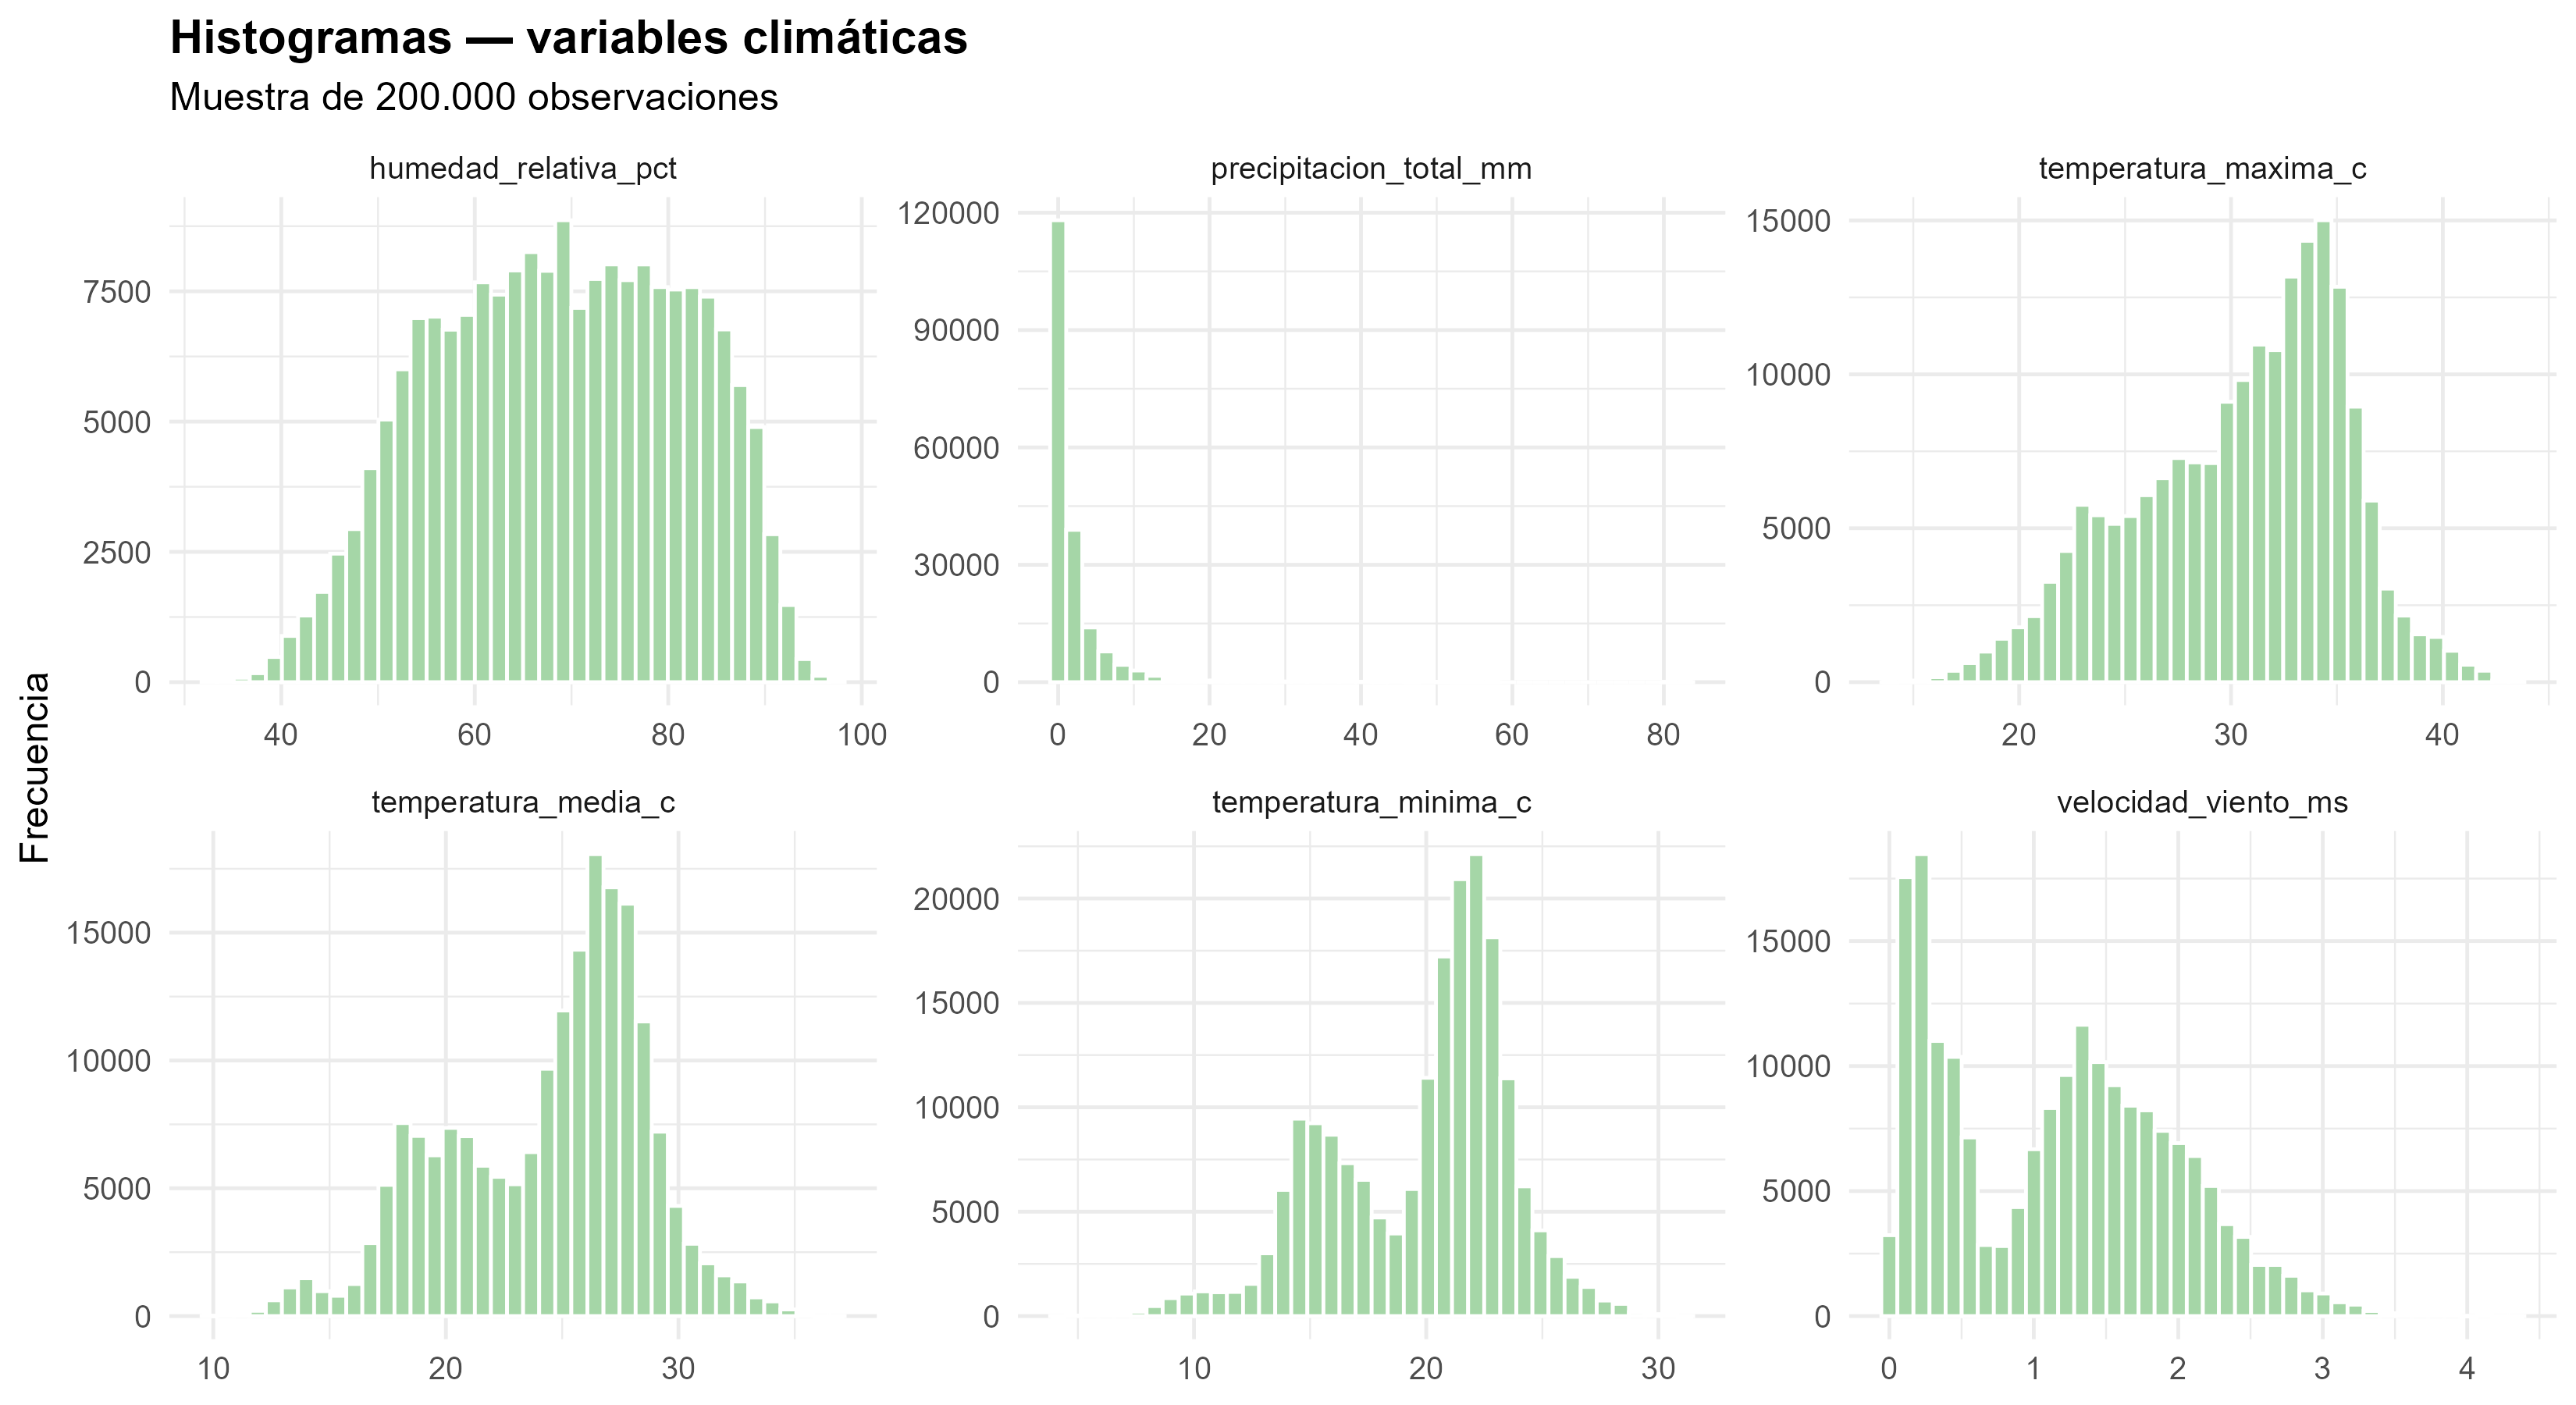
\includegraphics[width=0.95\textwidth]{img/histograma_valores_extremos_clima.png}
        \caption{Distribución de las variables climáticas: forma y cola (muestra de $200\,000$ observaciones).}
        \label{fig:histograma_clima}
    \end{figure}
    
    \subparagraph{Variables de severidad y continuidad diarias.} Estas variables están dominadas por ceros (días sin interrupción): el $99{.}94$~\% de las filas registra $0$, por lo que sobre el panel completo se cumple $Q_1 = Q_3 = 0$ y la regla de Tukey resulta poco informativa (marca como extremo cualquier día con evento, $0{.}06$~\% del panel); el CV del panel completo queda artificialmente inflado por la masa en cero. Por ello, el análisis relevante se realiza sobre los días con evento ($\text{valor} > 0$), donde se concentran $48\,375$ registros de afectación y $48\,364$ de continuidad. En este subconjunto las distribuciones son fuertemente asimétricas a la derecha y de alta dispersión relativa: la mediana de \texttt{CANTIDAD\_USUARIOS} es $23$ usuarios pero su máximo alcanza $34\,622$ (CV $= 3{.}97$); la \texttt{DURACION\_min} tiene mediana de $417$ minutos ($\approx 7$~horas) y un máximo de $332\,395$ minutos ($\approx 231$~días; CV $= 3{.}56$), sugerente de posibles inconsistencias de registro que se marcan para revisión. La regla de Tukey marca entre el $9$~\% y el $15$~\% de los días con evento como extremos, proporción esperable en distribuciones de cola pesada. La Tabla~\ref{tab:extremos_evento} resume estos resultados y las Figuras~\ref{fig:boxplot_evento} y~\ref{fig:histograma_evento} presentan los diagramas de caja e histogramas sobre los días con evento.
    
    \begin{table}[!htbp]
    \centering
    \small
    \caption{Valores extremos y dispersión relativa en severidad y continuidad (días con evento, $\text{valor} > 0$)}
    \label{tab:extremos_evento}
    \begin{tabular}{l r r r r r r}
    \toprule
    \textbf{Variable} & \textbf{$n$} & \textbf{Mediana} & \textbf{Máximo} & \textbf{CV} & \textbf{\% IQR 1.5} & \textbf{\% IQR 3.0} \\
    \midrule
    \texttt{CANTIDAD\_ELEMENTOS} & 48\,375 & 2   & 2\,469   & 3.15 & 14.91 & 11.78 \\
    \texttt{CANTIDAD\_USUARIOS}  & 48\,375 & 23  & 34\,622  & 3.97 & 14.50 & 10.83 \\
    \texttt{DURACION\_min}  & 48\,364 & 417 & 332\,395 & 3.56 & 8.94  & 5.36  \\
    \texttt{FRECUENCIA}          & 48\,364 & 1   & 6         & 0.15 & 1.96  & 1.96  \\
\bottomrule
    \end{tabular}
    \end{table}
    
    
    \begin{figure}[!htbp]
        \centering
        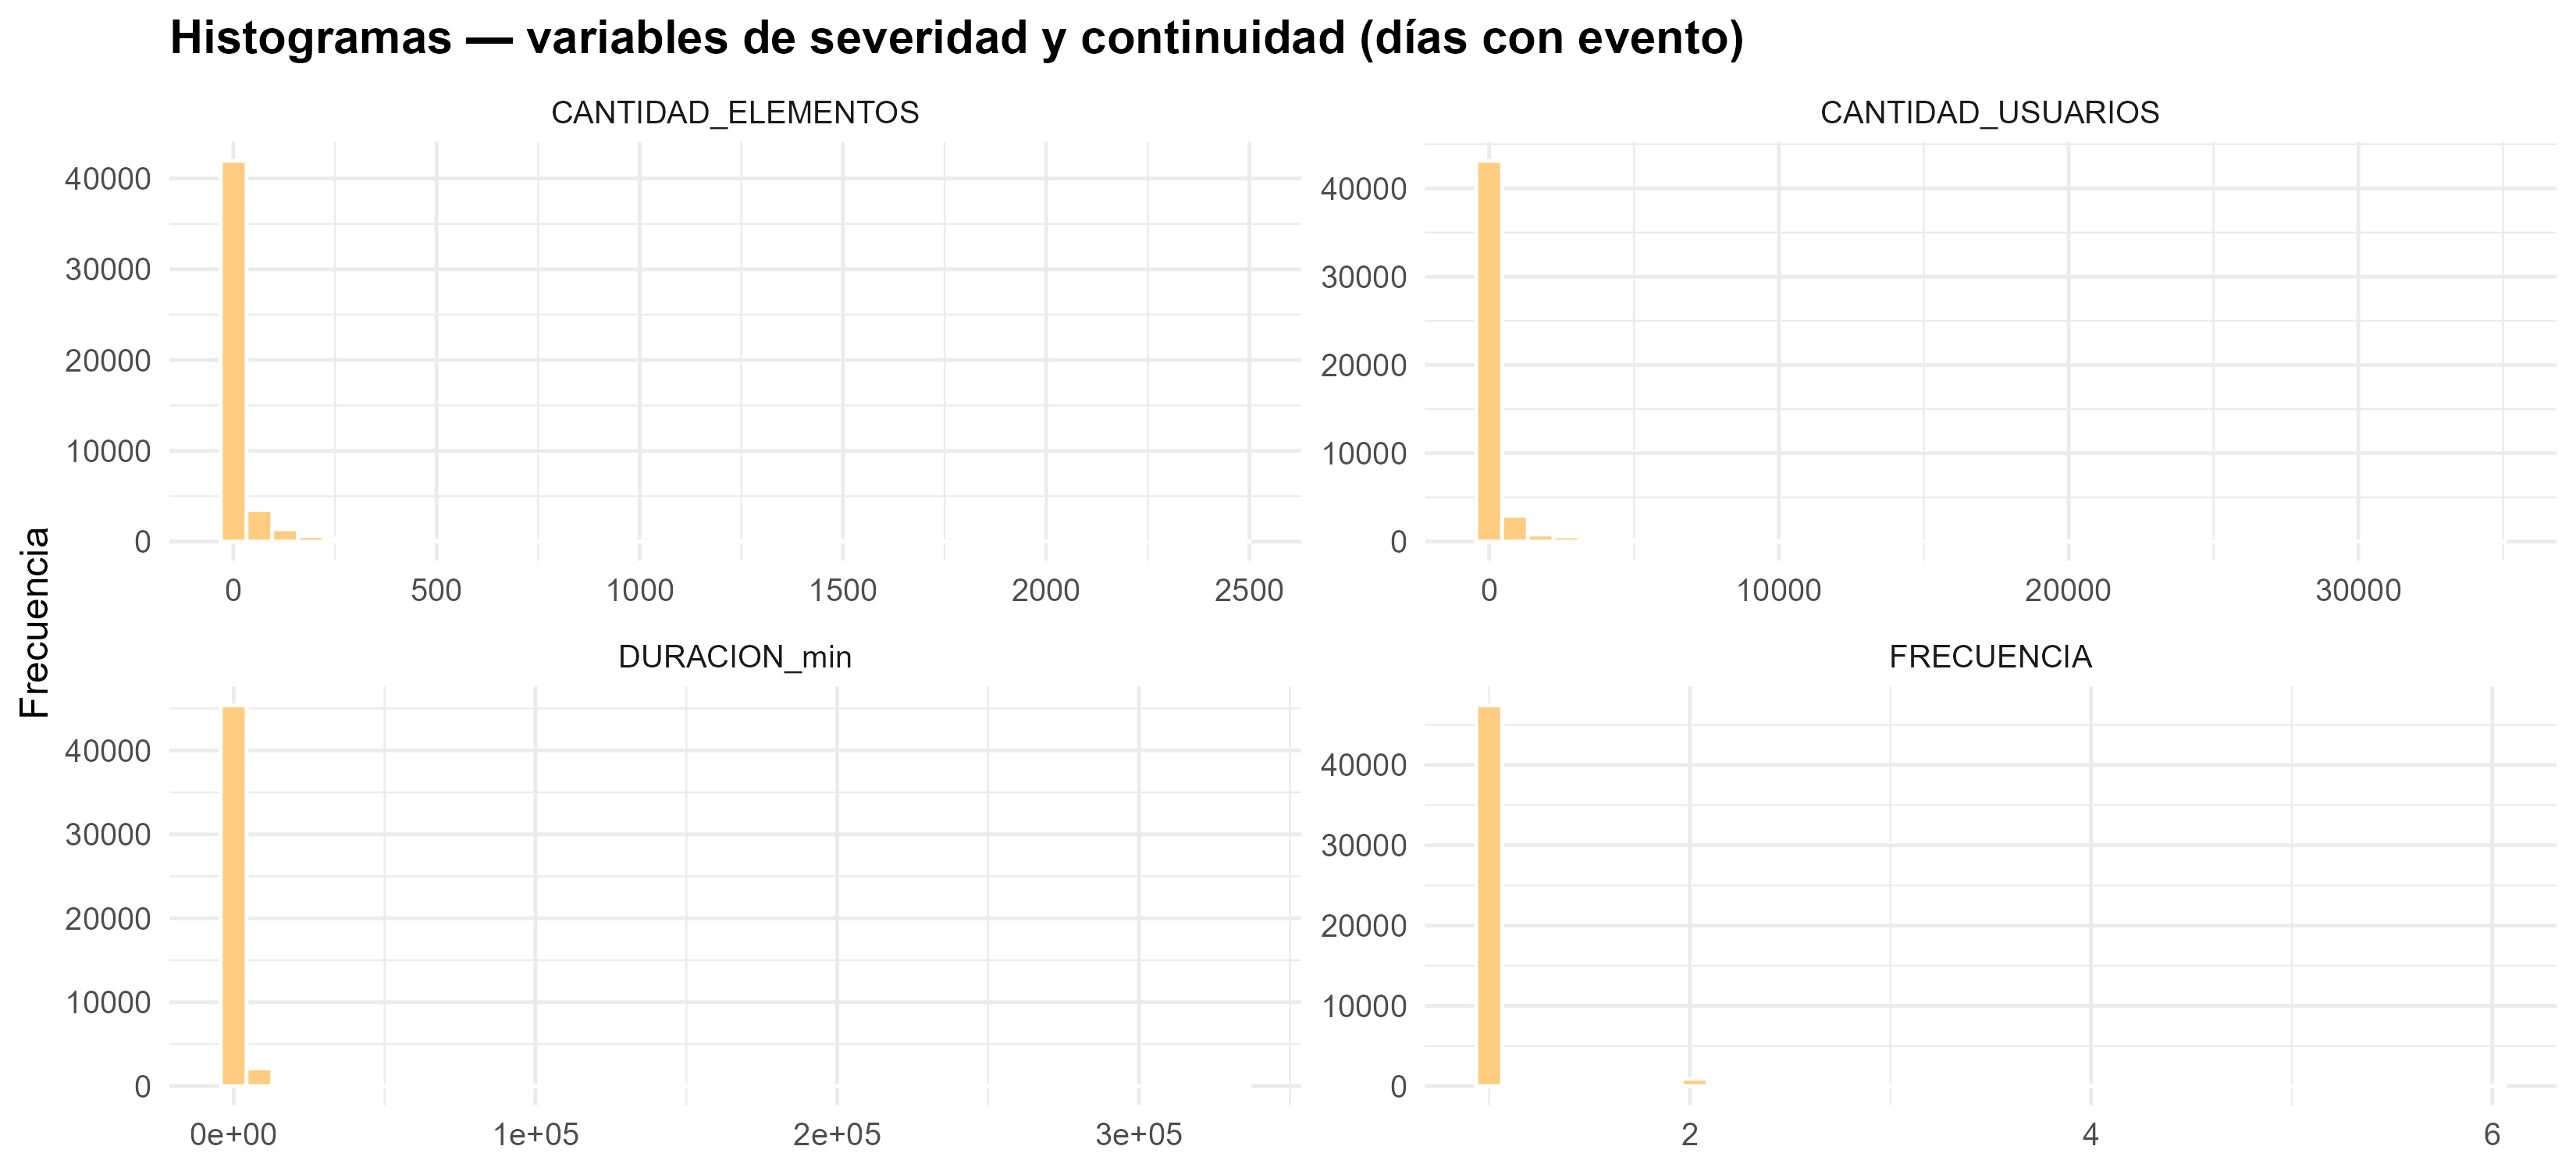
\includegraphics[width=0.95\textwidth]{img/histograma_valores_extremos_evento.png}
        \caption{Distribución de la severidad y continuidad en días con evento: forma y cola.}
        \label{fig:histograma_evento}
    \end{figure}
    
    \paragraph{Tabla agrupada cuadrante $\times$ semana.} Sobre \texttt{data\_agrupada.csv} (Sección~\ref{sec:agrupacion_cuadrante_semana}), con $N_{\mathrm{agr}} = 90\,128$ observaciones, se replicó el mismo esquema excluyendo \texttt{id\_cuadrante}, \texttt{latitud}, \texttt{longitud} y \texttt{altitud}. El procedimiento se documenta en el Apéndice~\ref{app:html-outliers-agrupada}.
    
    \subparagraph{Variables climáticas semanales.} El diagnóstico se realizó sobre la tabla completa. Las variables de temperatura y humedad presentan distribuciones aproximadamente simétricas, baja dispersión relativa (CV entre $0{.}16$ y $0{.}25$) y un porcentaje muy bajo de extremos bajo Tukey (entre $0$~\% y $0{.}03$~\%); con el factor $3{.}0$ no se identifican extremos severos. El viento semanal es más heterogéneo (CV $\approx 0{.}78$--$0{.}81$). La \texttt{precip\_total\_semana} constituye la excepción: al ser un acumulado semanal asimétrico a la derecha con CV $= 1{.}17$, la regla de Tukey marca el $6{.}21$~\% de las observaciones y la ampliada el $1{.}79$~\%, aunque la regla de percentiles solo señala el $0{.}99$~\%. Los valores señalados corresponden a semanas de lluvia intensa operativamente plausibles: el máximo observado es de $198{.}1$~mm acumulados en la semana, magnitud compatible con los registros de temporada de lluvia en la región. La Tabla~\ref{tab:extremos_clima_agrupada} resume estos resultados y las Figuras~\ref{fig:boxplot_clima_agrupada} y~\ref{fig:histograma_clima_agrupada} muestran los diagramas de caja y los histogramas sobre las $90\,128$ observaciones.
    
    \begin{table}[!htbp]
    \centering
    \small
    \caption{Valores extremos y dispersión relativa en variables climáticas semanales (tabla agrupada)}
    \label{tab:extremos_clima_agrupada}
    \begin{tabular}{l r r r r r}
    \toprule
    \textbf{Variable} & \textbf{Mediana} & \textbf{CV} & \textbf{\% IQR 1.5} & \textbf{\% IQR 3.0} & \textbf{\% P1--P99} \\
    \midrule
    \texttt{temp\_media\_semana}    & 24.84 & 0.19 & 0.00 & 0.00 & 1.95 \\
    \texttt{temp\_max\_semana}      & 32.72 & 0.17 & 0.00 & 0.00 & 1.99 \\
    \texttt{temp\_min\_semana}      & 18.95 & 0.25 & 0.03 & 0.00 & 1.96 \\
    \texttt{humedad\_media\_semana} & 72.28 & 0.16 & 0.00 & 0.00 & 1.97 \\
    \texttt{viento\_medio\_semana}  & 0.91  & 0.81 & 0.00 & 0.00 & 1.99 \\
    \texttt{viento\_max\_semana}    & 1.26  & 0.78 & 0.00 & 0.00 & 1.69 \\
    \texttt{precip\_total\_semana}  & 9.78  & 1.17 & 6.21 & 1.79 & 0.99 \\
    \bottomrule
    \end{tabular}
\end{table}

    
    \begin{figure}[!htbp]
        \centering
        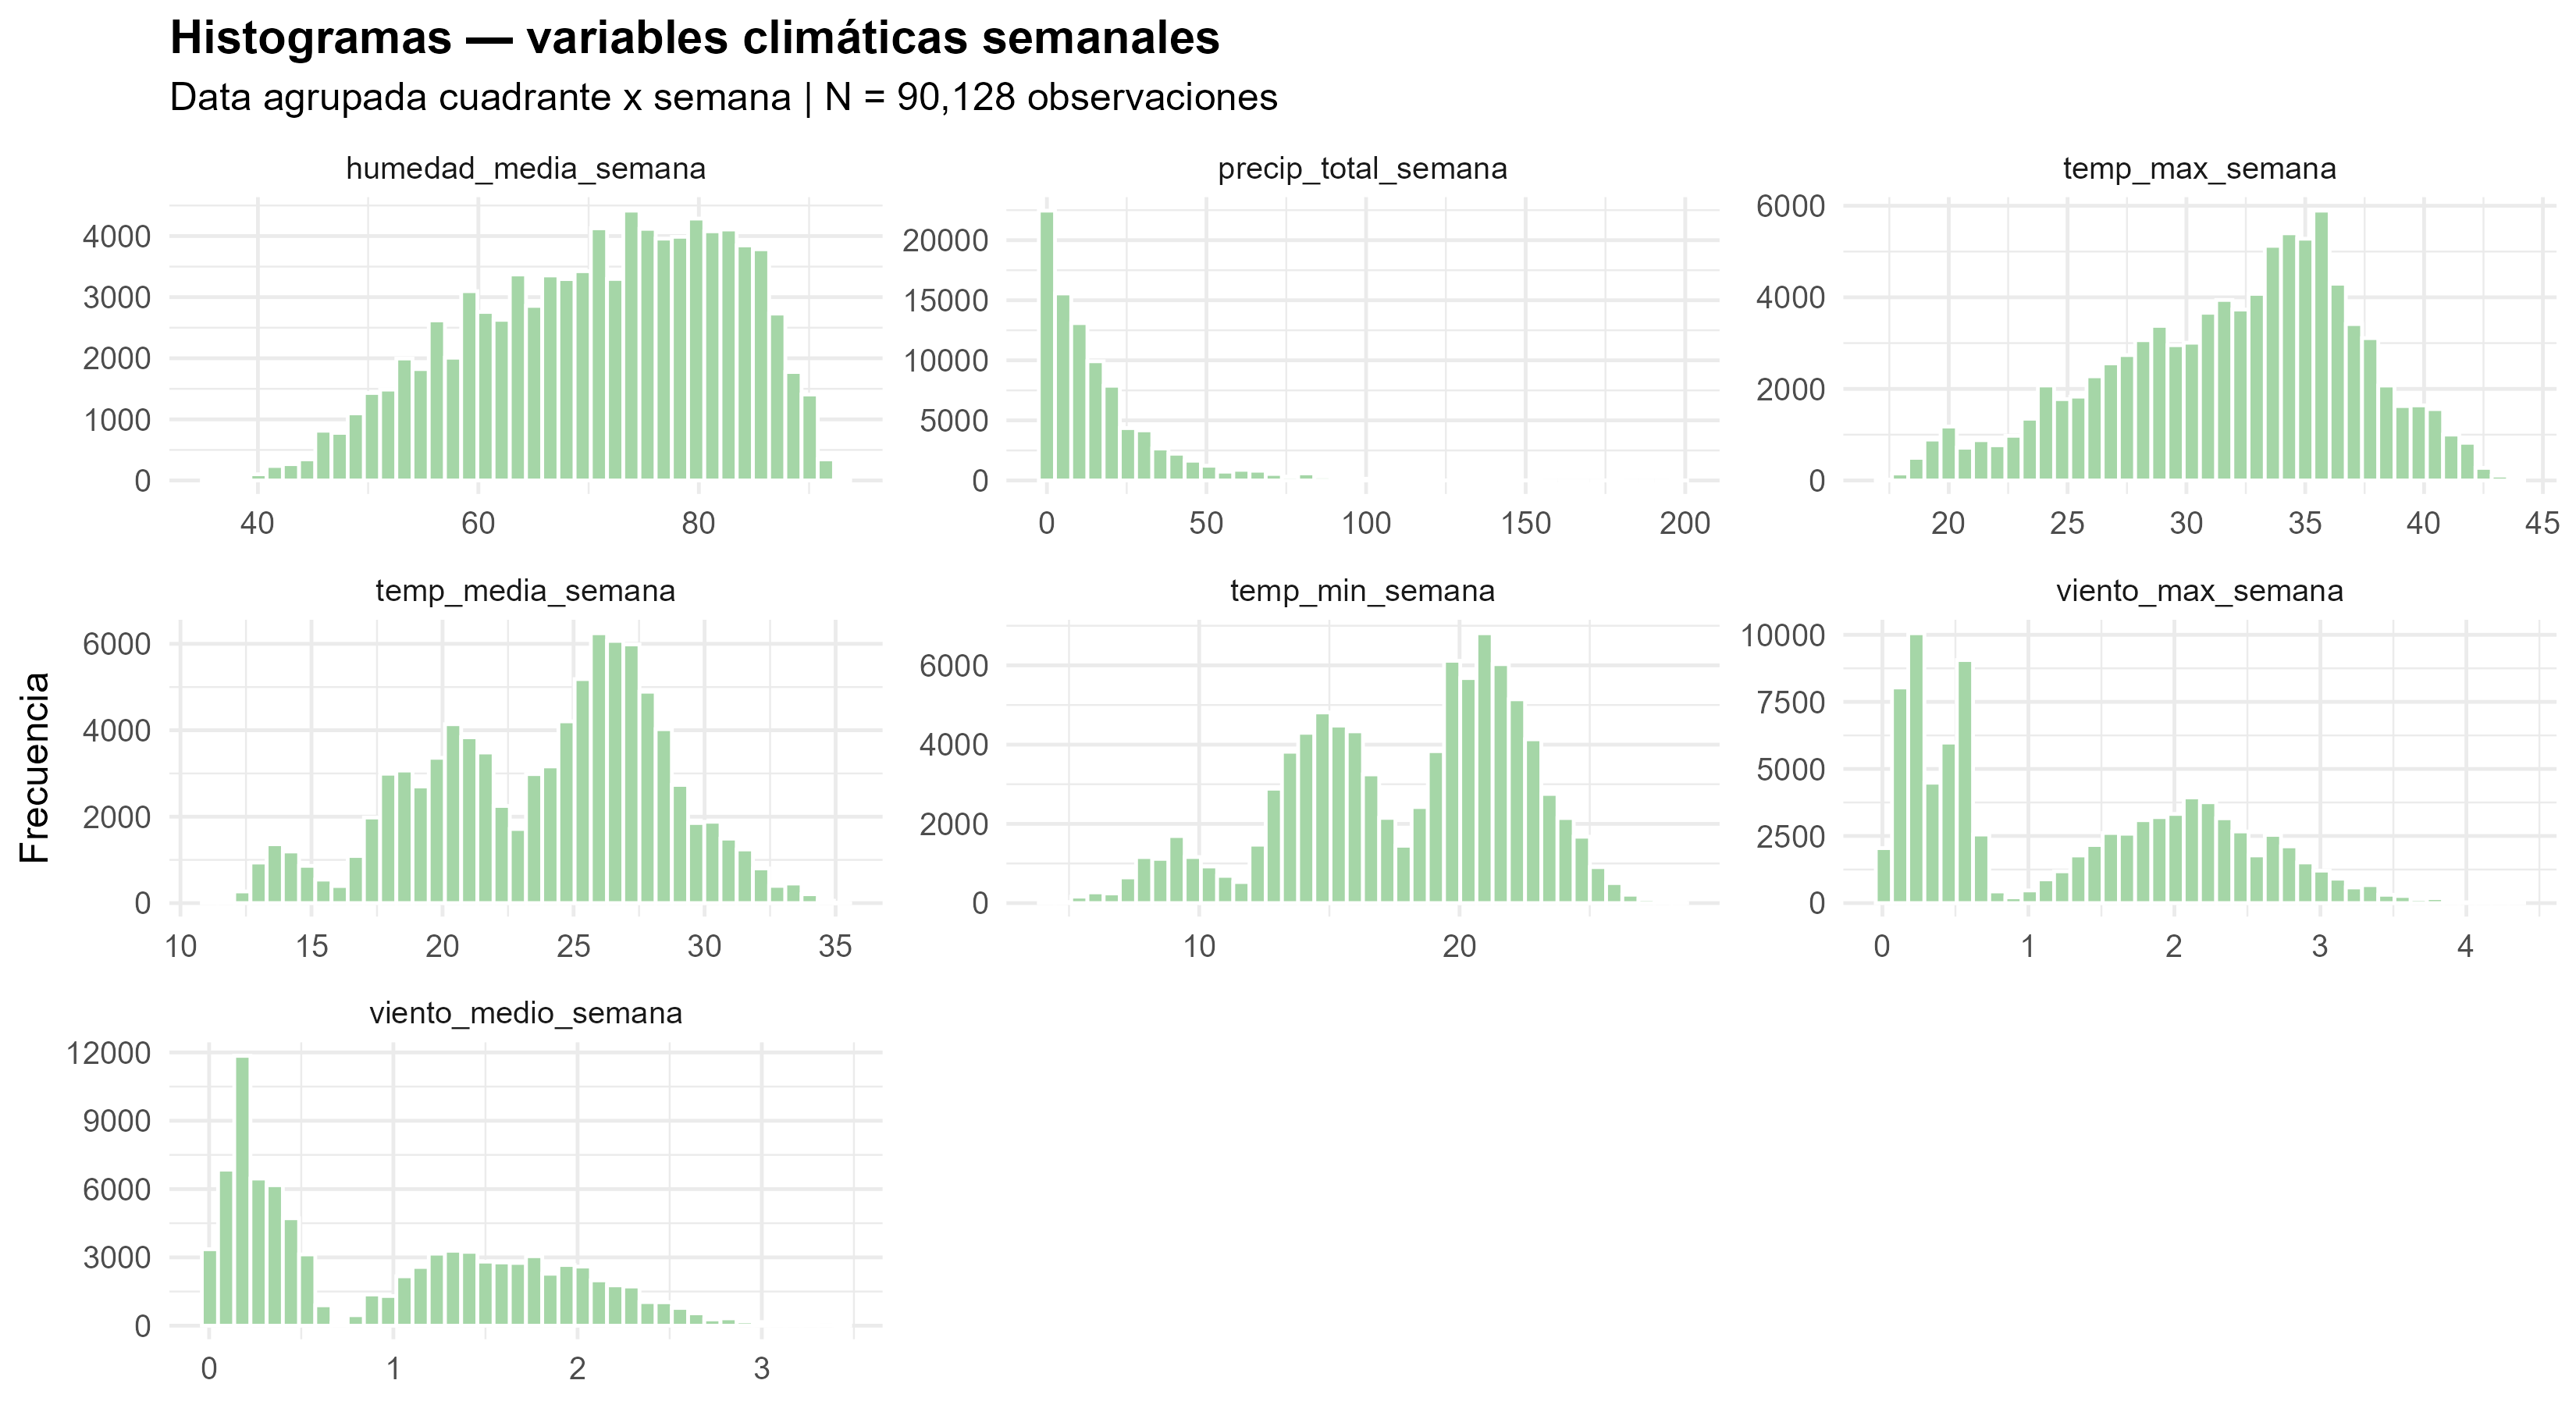
\includegraphics[width=0.95\textwidth]{img/histograma_valores_extremos_clima_agrupada.png}
        \caption{Distribución de las variables climáticas semanales: forma y cola ($N_{\mathrm{agr}} = 90\,128$).}
        \label{fig:histograma_clima_agrupada}
    \end{figure}
    
    \subparagraph{Variables de severidad y continuidad.} En la tabla completa persisten semanas sin interrupción registrada ($Q_1 = Q_3 = 0$ en \texttt{usuarios\_afectados}, \texttt{elementos\_afectados} y \texttt{n\_eventos}), por lo que la regla de Tukey sobre el total es poco informativa para esas variables y el CV del panel completo queda inflado por ceros (Tabla~\ref{tab:desc_evento_agrupada}). El análisis relevante se realiza sobre semanas con evento ($\text{valor} > 0$), con $22\,660$--$24\,800$ registros según la variable. En este subconjunto las distribuciones son fuertemente asimétricas a la derecha y de alta dispersión relativa: la mediana de \texttt{usuarios\_afectados} es $52$ usuarios pero su máximo alcanza $69\,928$ (CV $= 3{.}82$); \texttt{duracion\_total} tiene mediana de $19{.}7$~horas y un máximo de $2\,227$~horas ($\approx 93$~días acumulados; CV $= 1{.}73$). La regla de Tukey marca entre el $11{.}6$~\% y el $15{.}2$~\% de las semanas con evento como extremos, proporción esperable en distribuciones de cola pesada. La Tabla~\ref{tab:extremos_evento_agrupada} resume estos resultados y las Figuras~\ref{fig:boxplot_evento_agrupada} y~\ref{fig:histograma_evento_agrupada} presentan los diagramas de caja e histogramas.

\begin{table}[!htbp]
\centering
    \small
    \caption{Valores extremos y dispersión relativa en severidad y continuidad (semanas con evento, $\text{valor} > 0$)}
    \label{tab:extremos_evento_agrupada}
    \begin{tabular}{l r r r r r r}
    \toprule
    \textbf{Variable} & \textbf{$n$} & \textbf{Mediana} & \textbf{Máximo} & \textbf{CV} & \textbf{\% IQR 1.5} & \textbf{\% IQR 3.0} \\
    \midrule
    \texttt{usuarios\_afectados}  & 22\,660 & 52    & 69\,928 & 3.82 & 15.16 & 11.21 \\
    \texttt{elementos\_afectados} & 22\,660 & 7     & 3\,626  & 2.75 & 15.00 & 10.70 \\
    \texttt{duracion\_total}      & 24\,800 & 19.7  & 2\,227  & 1.73 & 11.56 & 4.25  \\
    \texttt{n\_eventos}            & 22\,659 & 1     & 58       & 1.08 & 14.53 & 5.73  \\
    \bottomrule
    \end{tabular}
    \end{table}
    
    
    \begin{figure}[!htbp]
        \centering
        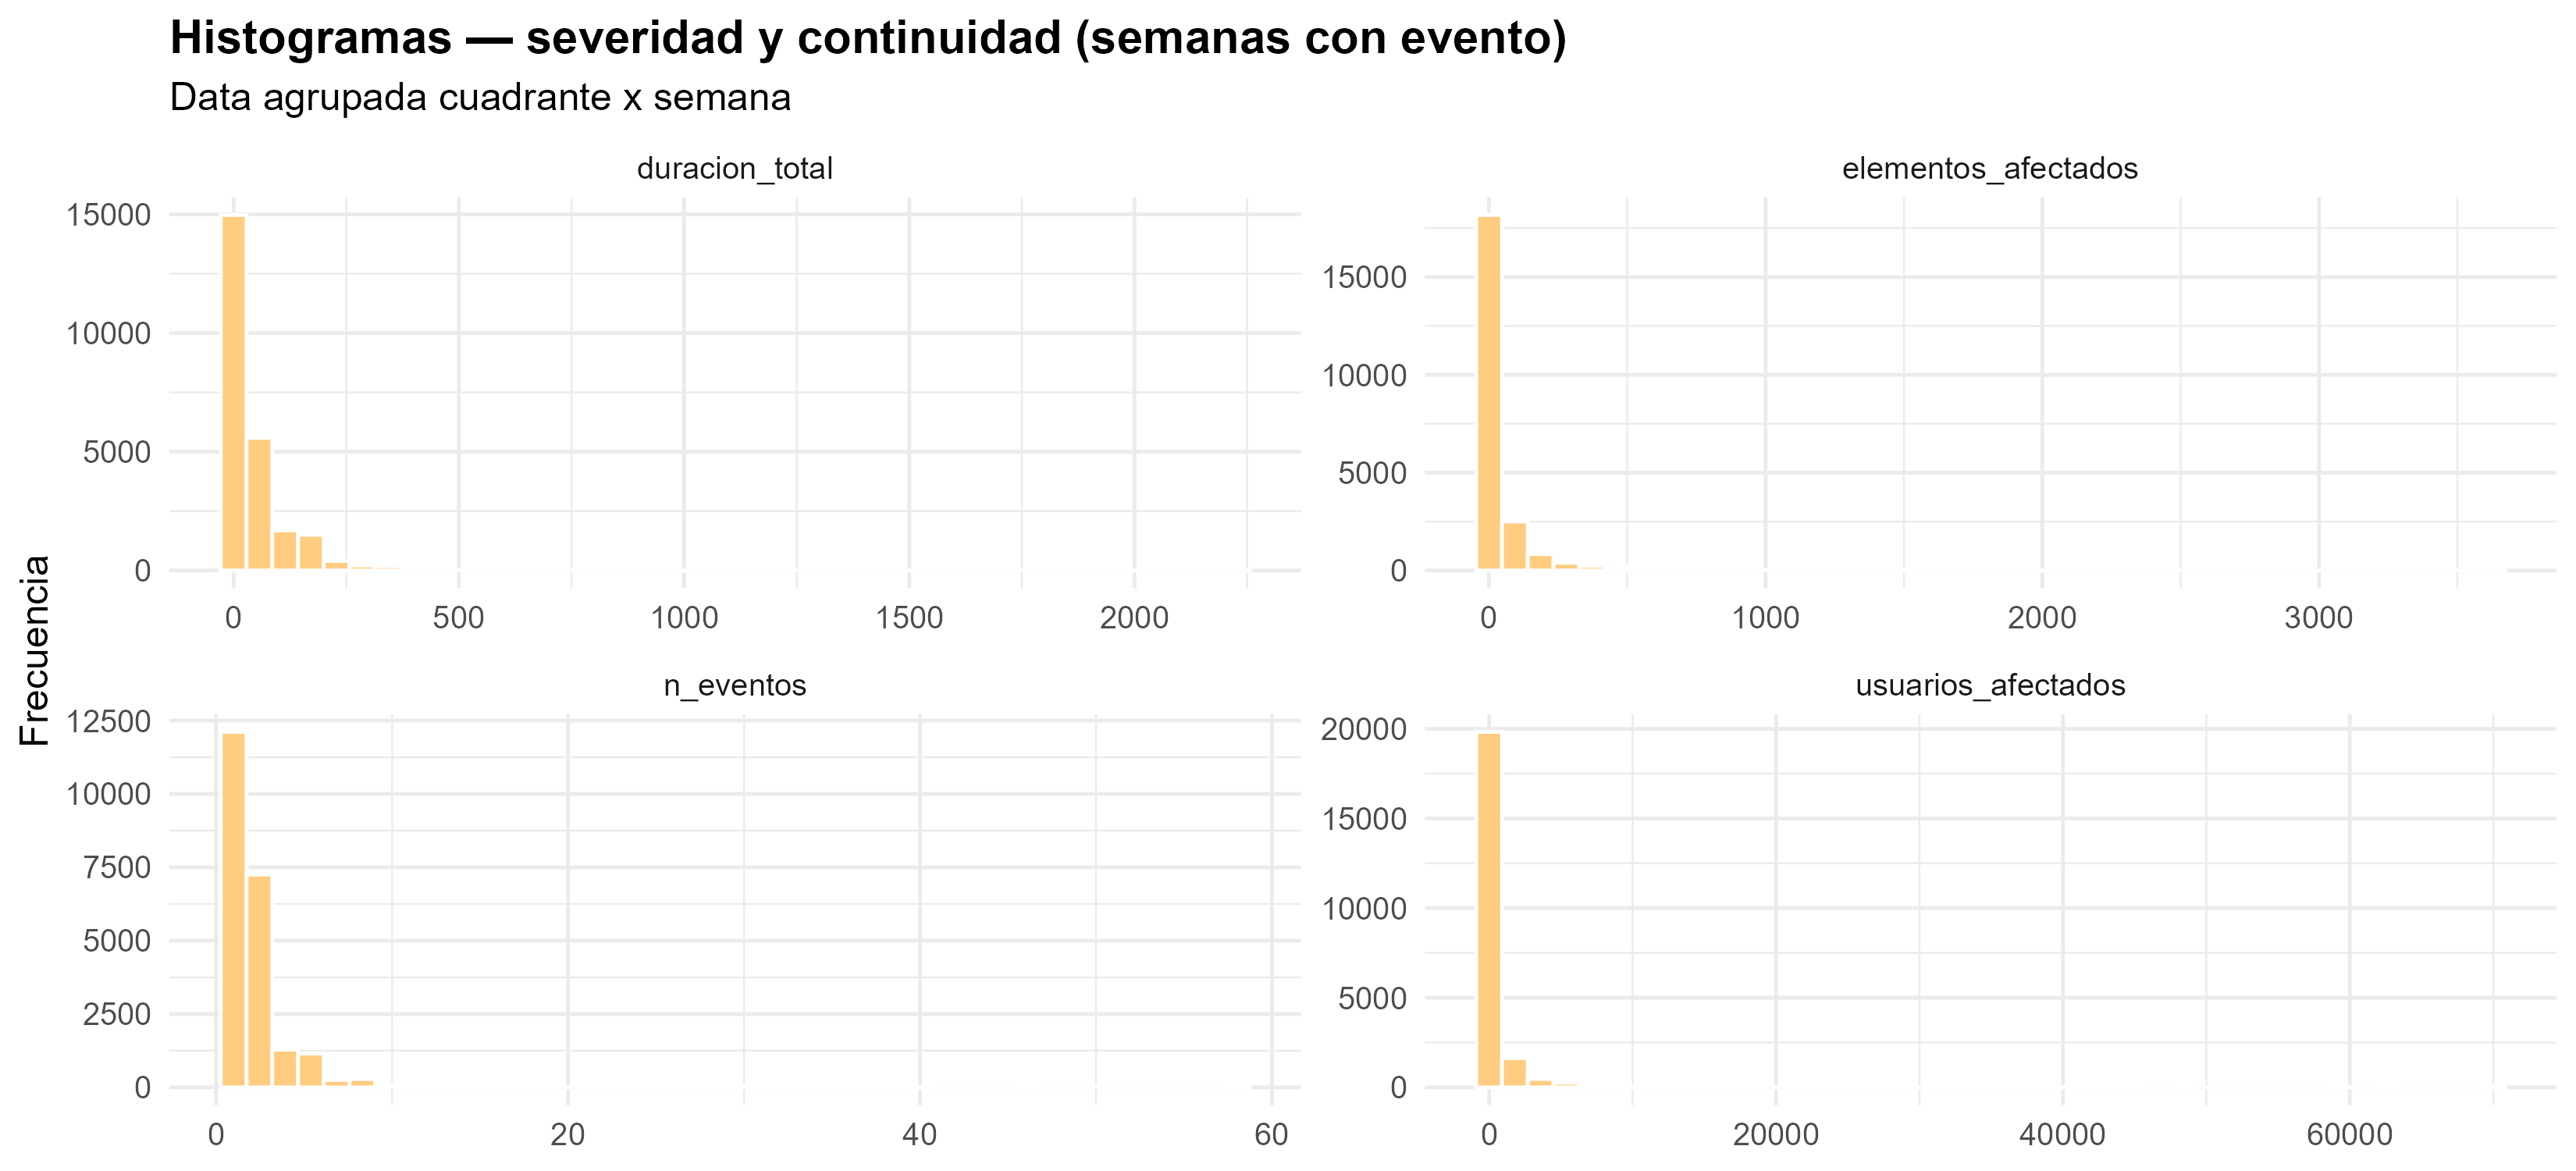
\includegraphics[width=0.95\textwidth]{img/histograma_valores_extremos_evento_agrupada.png}
        \caption{Distribución de la severidad y continuidad en semanas con evento: forma y cola.}
        \label{fig:histograma_evento_agrupada}
    \end{figure}
    
    \noindent En síntesis, en el grano cuadrante~$\times$~semana los extremos climáticos son escasos y operativamente plausibles (con la precipitación acumulada como única variable de asimetría apreciable y CV superior a la unidad), mientras que en severidad y continuidad la cola pesada y el CV condicionado a semanas con evento reflejan semanas de alta afectación o múltiples eventos en un mismo cuadrante. No se aplican transformaciones ni exclusiones en esta etapa; las decisiones de tratamiento se documentan y ejecutan en la Etapa~4 a partir de este diagnóstico sobre la tabla de análisis.
    
\subsection{Cálculo de estadísticos descriptivos}
\label{sec:estadisticos_descriptivos}
    Tras el diagnóstico de completitud (Sección~\ref{sec:identificacion_datos_faltantes}) y el análisis de valores extremos (Sección~\ref{sec:identificacion_valores_extremos}), se calculó un conjunto sistemático de estadísticos descriptivos sobre la tabla de análisis \texttt{data\_agrupada.csv} (Sección~\ref{sec:agrupacion_cuadrante_semana}), con $N_{\mathrm{agr}} = 90\,128$ observaciones cuadrante~$\times$~semana. Se excluyeron las llaves y coordenadas (\texttt{id\_cuadrante}, \texttt{latitud}, \texttt{longitud}, \texttt{altitud}) y se evaluaron las $11$ variables numéricas de severidad, clima semanal y continuidad. El procedimiento reproducible se documenta en el Apéndice~\ref{app:html-descriptivos}.
    
    Para cada variable se reportaron: (i)~medidas de tendencia central (media, mediana y moda); (ii)~medidas de dispersión (rango, varianza, desviación estándar y coeficiente de variación; Sección~\ref{sec:metodos-modelos}); (iii)~medidas de posición (cuartiles, deciles y percentiles P1, P5, P95 y P99); (iv)~medidas de forma (asimetría y curtosis con exceso); y (v)~distribución de frecuencias de la categoría derivada \emph{actividad semanal del cuadrante}, construida a partir de \texttt{n\_eventos} (sin eventos; $1$ evento; $2$--$5$ eventos; más de $5$ eventos). Las Figuras~\ref{fig:histograma_descriptivo_agrupada} y~\ref{fig:boxplot_descriptivo_agrupada} presentan la vista panorámica de las $11$ variables mediante histogramas y diagramas de caja.
    
    \begin{figure}[!htbp]
        \centering
        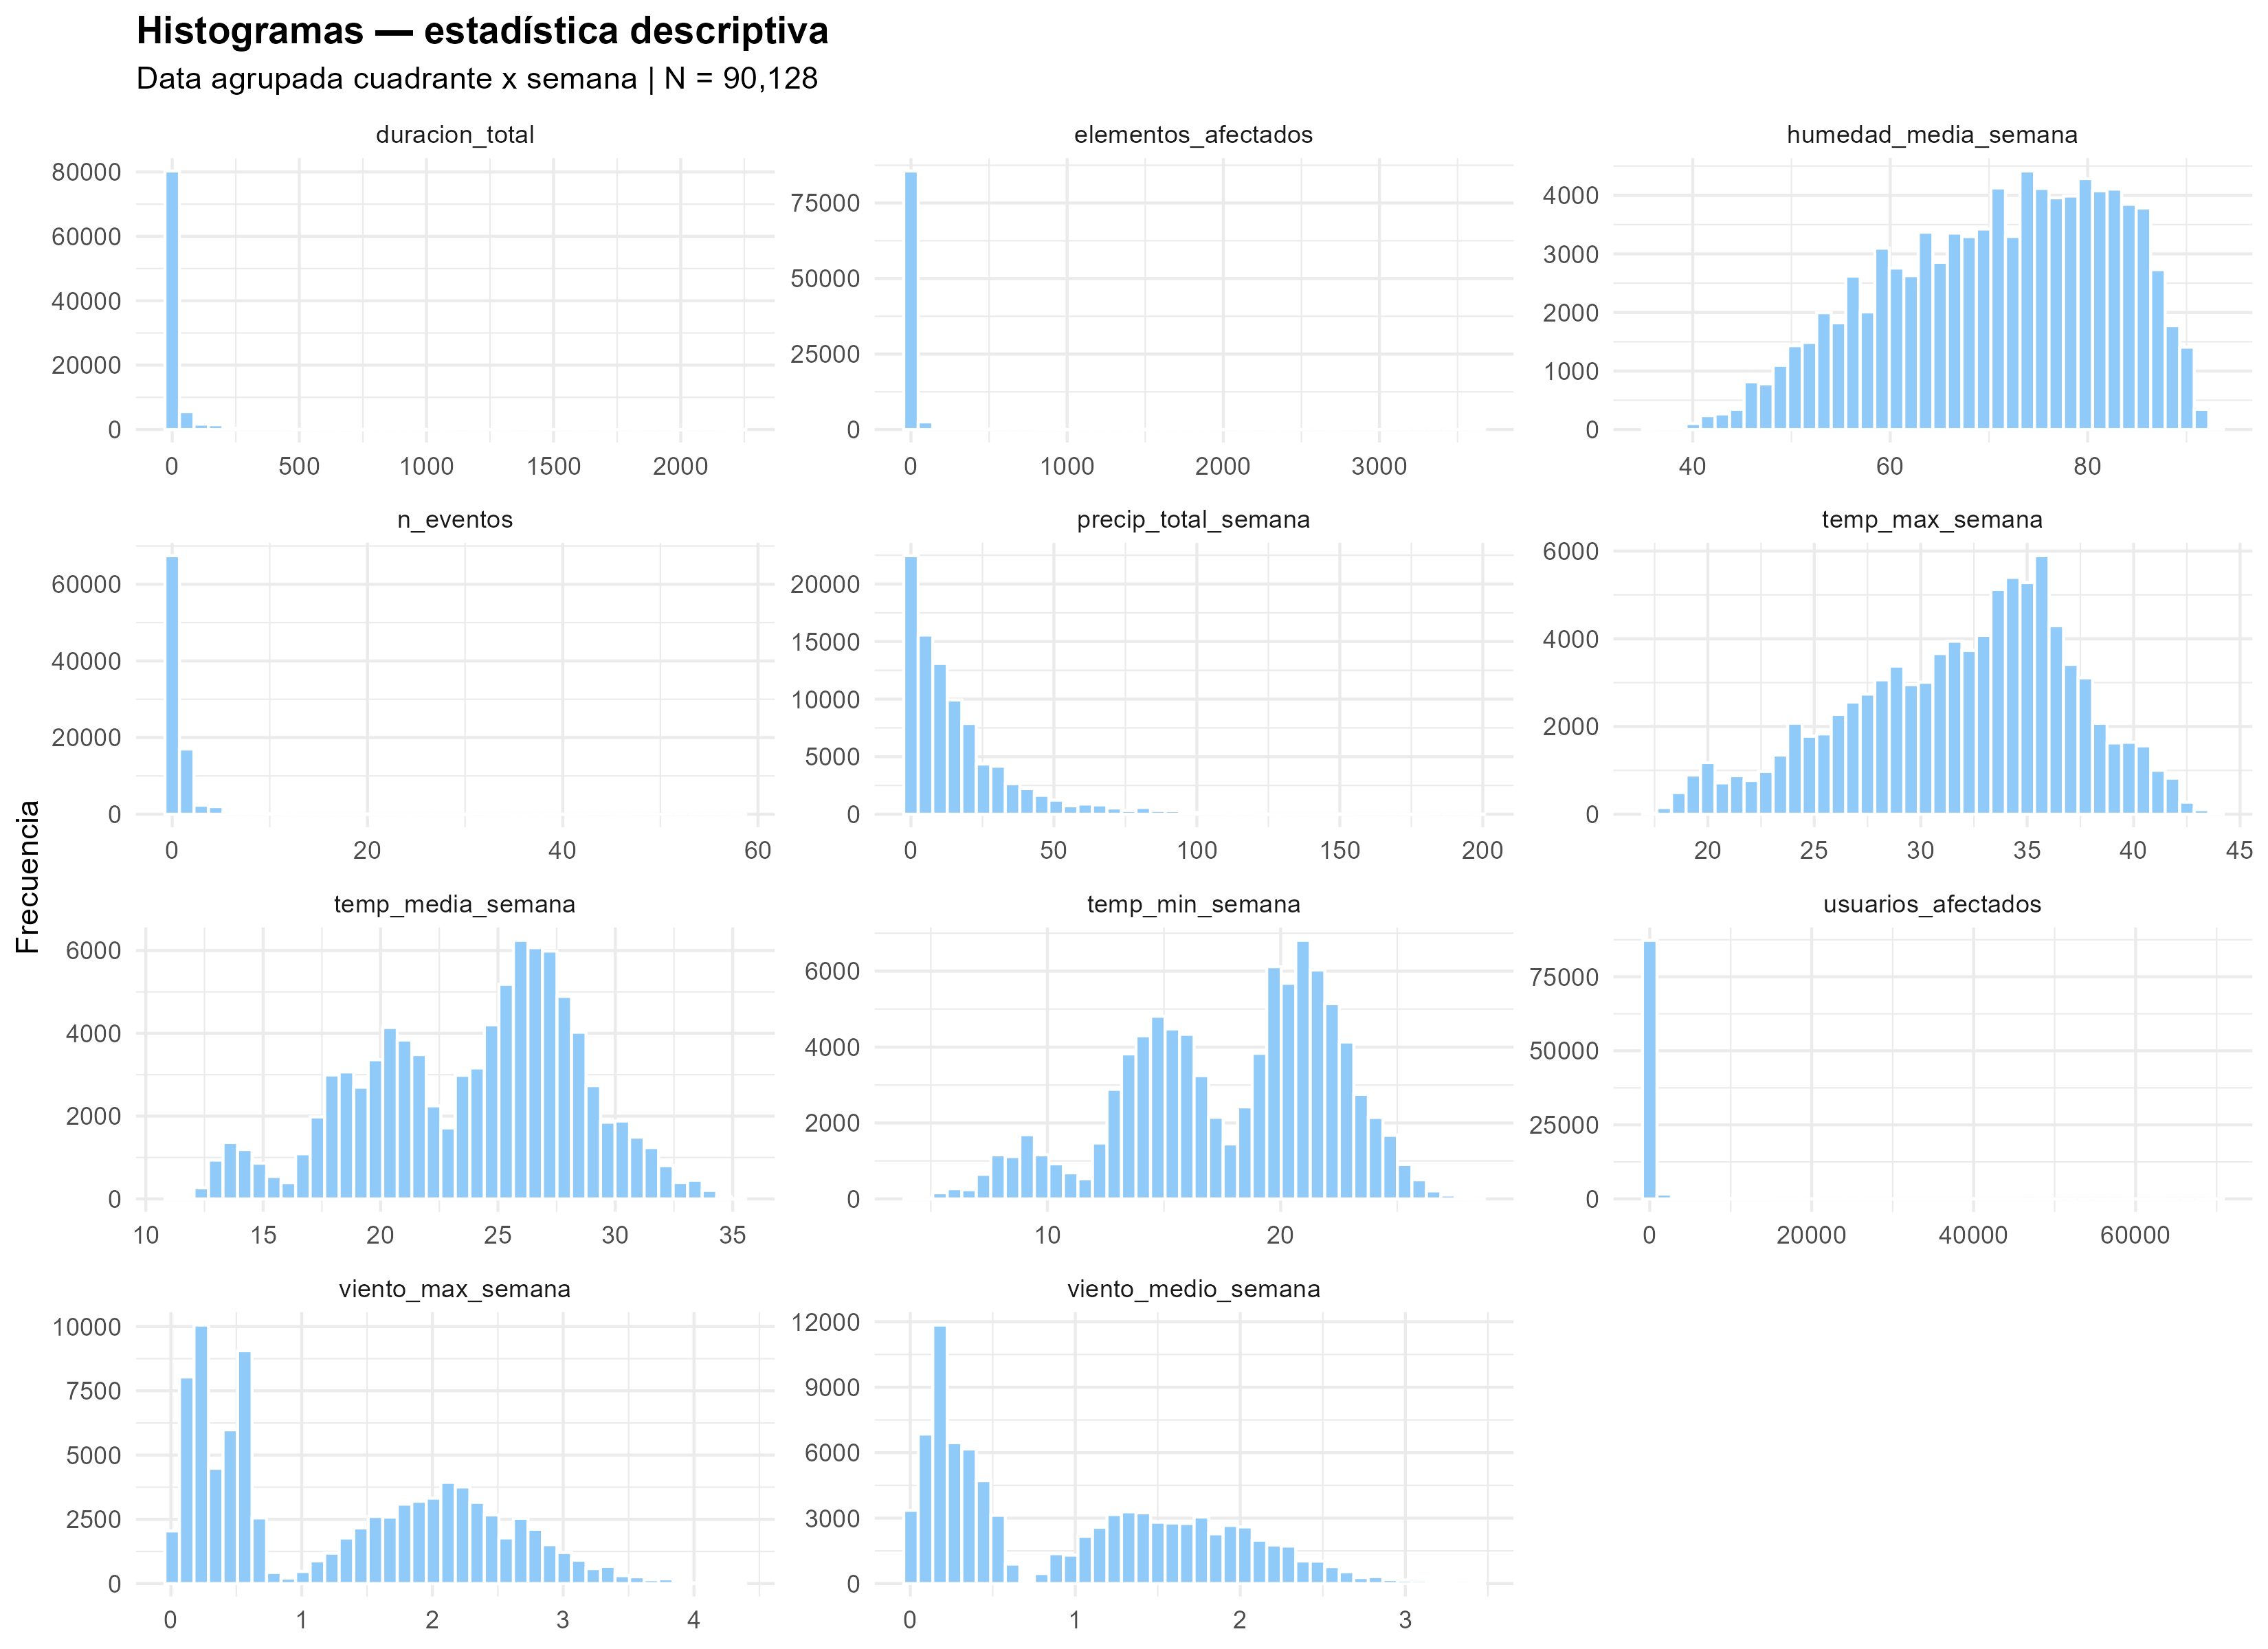
\includegraphics[width=0.95\textwidth]{img/histograma_descriptivo_agrupada.png}
        \caption{Distribución de las variables numéricas de la tabla agrupada: forma y cola ($N_{\mathrm{agr}} = 90\,128$).}
        \label{fig:histograma_descriptivo_agrupada}
    \end{figure}
    
    
    \paragraph{Variables climáticas semanales.} Las siete variables meteorológicas agregadas presentan distribuciones aproximadamente simétricas y baja dispersión relativa: el coeficiente de variación (CV) se ubica entre $0{.}16$ (\texttt{humedad\_media\_semana}) y $0{.}81$ (\texttt{viento\_medio\_semana}). La temperatura media semanal tiene mediana de $24{.}8$~\textdegree C (media $23{.}8$~\textdegree C; $Q_1$--$Q_3$: $20{.}4$--$27{.}2$~\textdegree C) y asimetría cercana a cero ($-0{.}37$). La humedad relativa media semanal concentra la mediana en $72{.}3$~\% (CV $= 0{.}16$). La excepción es \texttt{precip\_total\_semana}: acumulado semanal con mediana de $9{.}8$~mm, media de $16{.}0$~mm, CV $= 1{.}17$ y asimetría positiva ($1{.}98$), con un recorrido de $0$ a $198{.}1$~mm y un percentil $99$ de $85{.}1$~mm que corresponde a semanas de lluvia intensa puntuales. La Tabla~\ref{tab:desc_clima_agrupada} resume tendencia central y dispersión; la Figura~\ref{fig:densidad_clima_agrupada} muestra las curvas de densidad.
    
    \begin{table}[!htbp]
    \centering
\small
    \caption{Estadísticos descriptivos de variables climáticas semanales (tabla agrupada)}
    \label{tab:desc_clima_agrupada}
    \begin{tabular}{l r r r r r}
    \toprule
    \textbf{Variable} & \textbf{Media} & \textbf{Mediana} & \textbf{Desv. est.} & \textbf{CV} & \textbf{Asimetría} \\
    \midrule
    \texttt{temp\_media\_semana}    & 23.8  & 24.8 & 4.63  & 0.19 & $-0{.}37$ \\
    \texttt{temp\_max\_semana}      & 31.9  & 32.7 & 5.29  & 0.17 & $-0{.}44$ \\
    \texttt{temp\_min\_semana}      & 17.9  & 19.0 & 4.49  & 0.25 & $-0{.}49$ \\
    \texttt{humedad\_media\_semana} & 70.9  & 72.3 & 11.5  & 0.16 & $-0{.}36$ \\
    \texttt{viento\_medio\_semana}  & 0.99  & 0.91 & 0.80  & 0.81 & 0.44 \\
    \texttt{viento\_max\_semana}    & 1.30  & 1.26 & 1.01  & 0.78 & 0.37 \\
    \texttt{precip\_total\_semana}  & 16.0  & 9.8  & 18.7  & 1.17 & 1.98 \\
    \bottomrule
    \end{tabular}
    \end{table}
    
    \begin{figure}[!htbp]
        \centering
        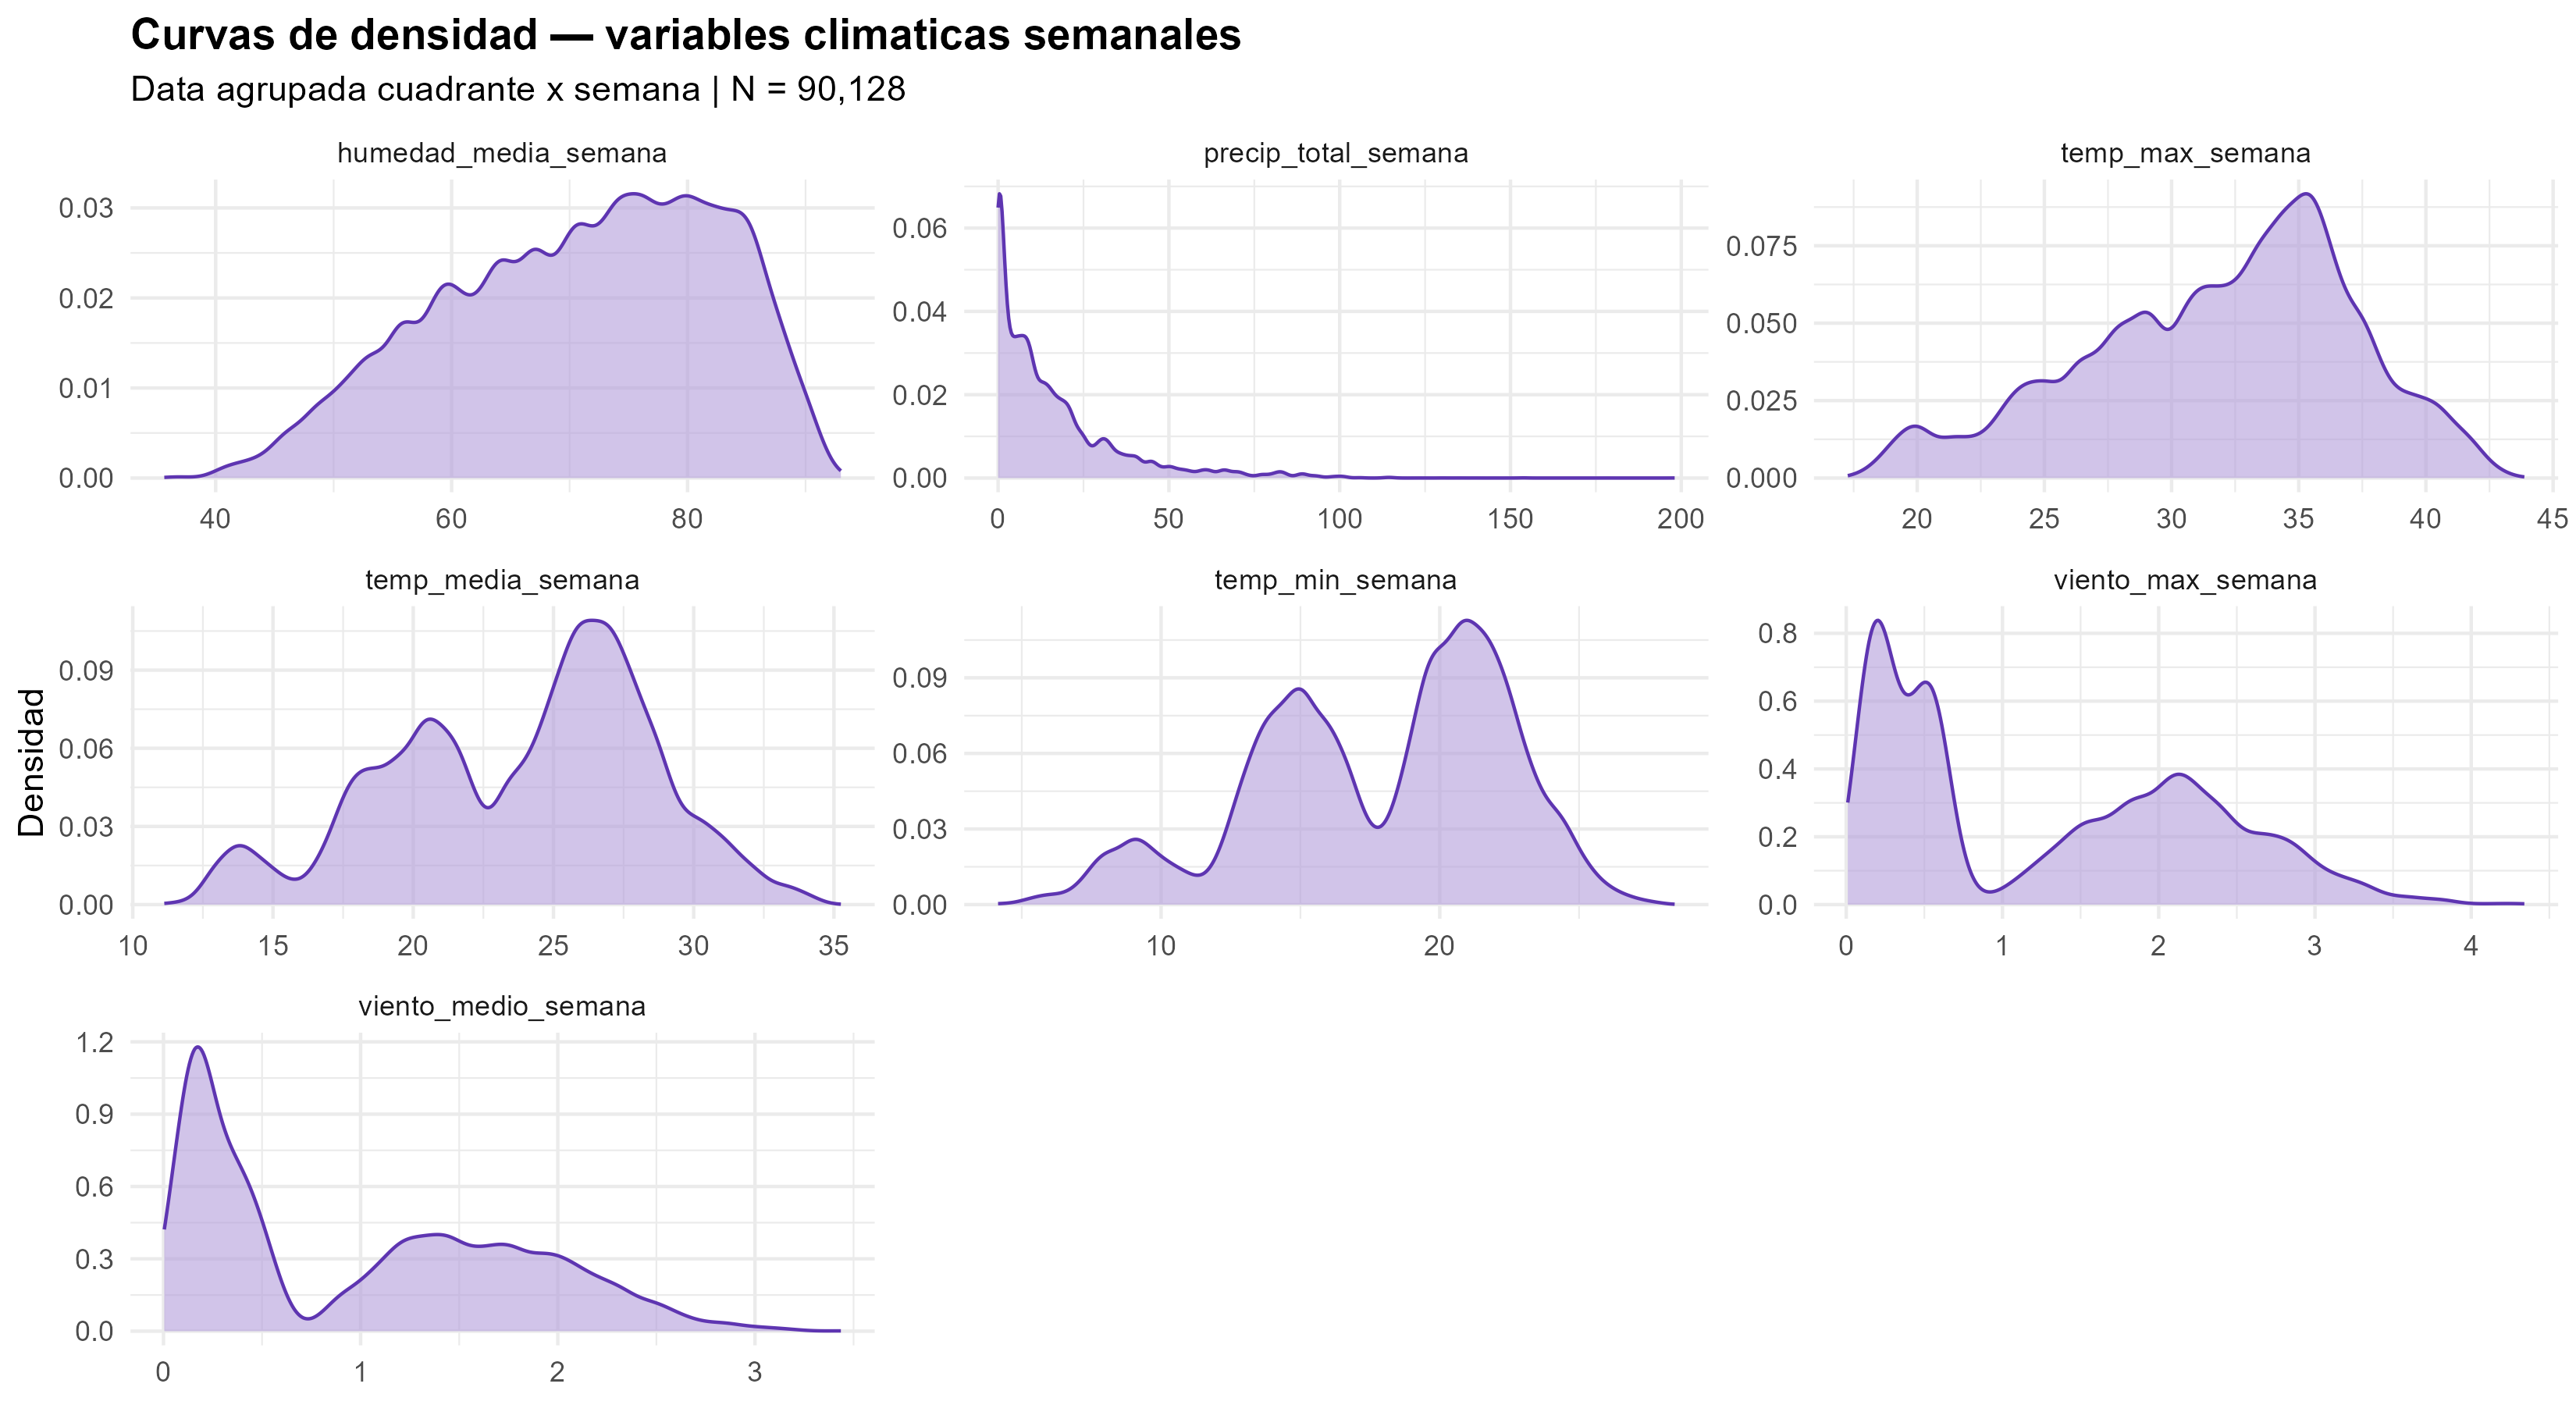
\includegraphics[width=0.95\textwidth]{img/curvas_densidad_clima_agrupada.png}
        \caption{Forma de la distribución de las variables climáticas semanales ($N_{\mathrm{agr}} = 90\,128$).}
        \label{fig:densidad_clima_agrupada}
    \end{figure}
    
    \paragraph{Variables de severidad y continuidad.} Las cuatro variables operativas están dominadas por ceros: la mediana de \texttt{usuarios\_afectados}, \texttt{elementos\_afectados}, \texttt{n\_eventos} y \texttt{duracion\_total} es $0$ en el $74{.}9$~\% de las semanas-cuadrante sin eventos registrados (Tabla~\ref{tab:frecuencias_actividad_agrupada}; Figuras~\ref{fig:barras_actividad_agrupada} y~\ref{fig:pastel_actividad_agrupada}). Cuando ocurre al menos un evento, las distribuciones son fuertemente leptocúrticas y con cola derecha pesada: \texttt{usuarios\_afectados} alcanza un máximo de $69\,928$ usuarios (media $156{.}1$; CV del panel completo $= 7{.}81$, inflado por ceros; CV condicionado a semanas con evento $= 3{.}82$); \texttt{duracion\_total} un máximo de $2\,227$~horas acumuladas en la semana (media $13{.}7$~h; CV completo $= 3{.}67$; CV condicionado $= 1{.}73$). La Tabla~\ref{tab:desc_evento_agrupada} resume las medidas principales del panel completo; la Tabla~\ref{tab:extremos_evento_agrupada} reporta el CV condicionado; la Figura~\ref{fig:densidad_evento_agrupada} presenta las densidades en escala logarítmica desplazada (Sección~\ref{sec:metodos-modelos}) para semanas con evento.
    
    \begin{table}[!htbp]
    \centering
    \small
    \caption{Estadísticos descriptivos de severidad y continuidad (tabla agrupada; panel completo)}
    \label{tab:desc_evento_agrupada}
    \begin{tabular}{l r r r r r r}
\toprule
    \textbf{Variable} & \textbf{Media} & \textbf{Mediana} & \textbf{Máx.} & \textbf{CV} & \textbf{Asimetría} & \textbf{$Q_3$} \\
\midrule
    \texttt{usuarios\_afectados}  & 156.1 & 0 & 69\,928 & 7.81 & 20.6 & 1 \\
    \texttt{elementos\_afectados} & 12.0  & 0 & 3\,626  & 5.74 & 14.1 & 1 \\
    \texttt{n\_eventos}            & 0.55  & 0 & 58       & 2.76 & 8.18 & 1 \\
    \texttt{duracion\_total}      & 13.7  & 0 & 2\,227  & 3.67 & 10.2 & 2.5 \\
    \bottomrule
    \end{tabular}
    
    \noindent\textit{Nota:} el CV del panel completo queda inflado por la cero-inflación; el CV condicionado a semanas con evento se reporta en la Tabla~\ref{tab:extremos_evento_agrupada}.
    \end{table}
    
    \begin{table}[!htbp]
    \centering
    \small
    \caption{Distribución de frecuencias por actividad semanal del cuadrante}
    \label{tab:frecuencias_actividad_agrupada}
    \begin{tabular}{l r r r}
    \toprule
    \textbf{Categoría (\texttt{n\_eventos})} & \textbf{Frec. absoluta} & \textbf{Frec. relativa (\%)} & \textbf{Frec. acumulada (\%)} \\
    \midrule
    Sin eventos           & 67\,469 & 74.86 & 74.86 \\
    $1$ evento            & 12\,115 & 13.44 & 88.30 \\
    $2$ a $5$ eventos     &  9\,246 & 10.26 & 98.56 \\
    Más de $5$ eventos    &  1\,298 &  1.44 & 100.00 \\
\bottomrule
    \end{tabular}
    \end{table}
    
    \begin{figure}[!htbp]
        \centering
        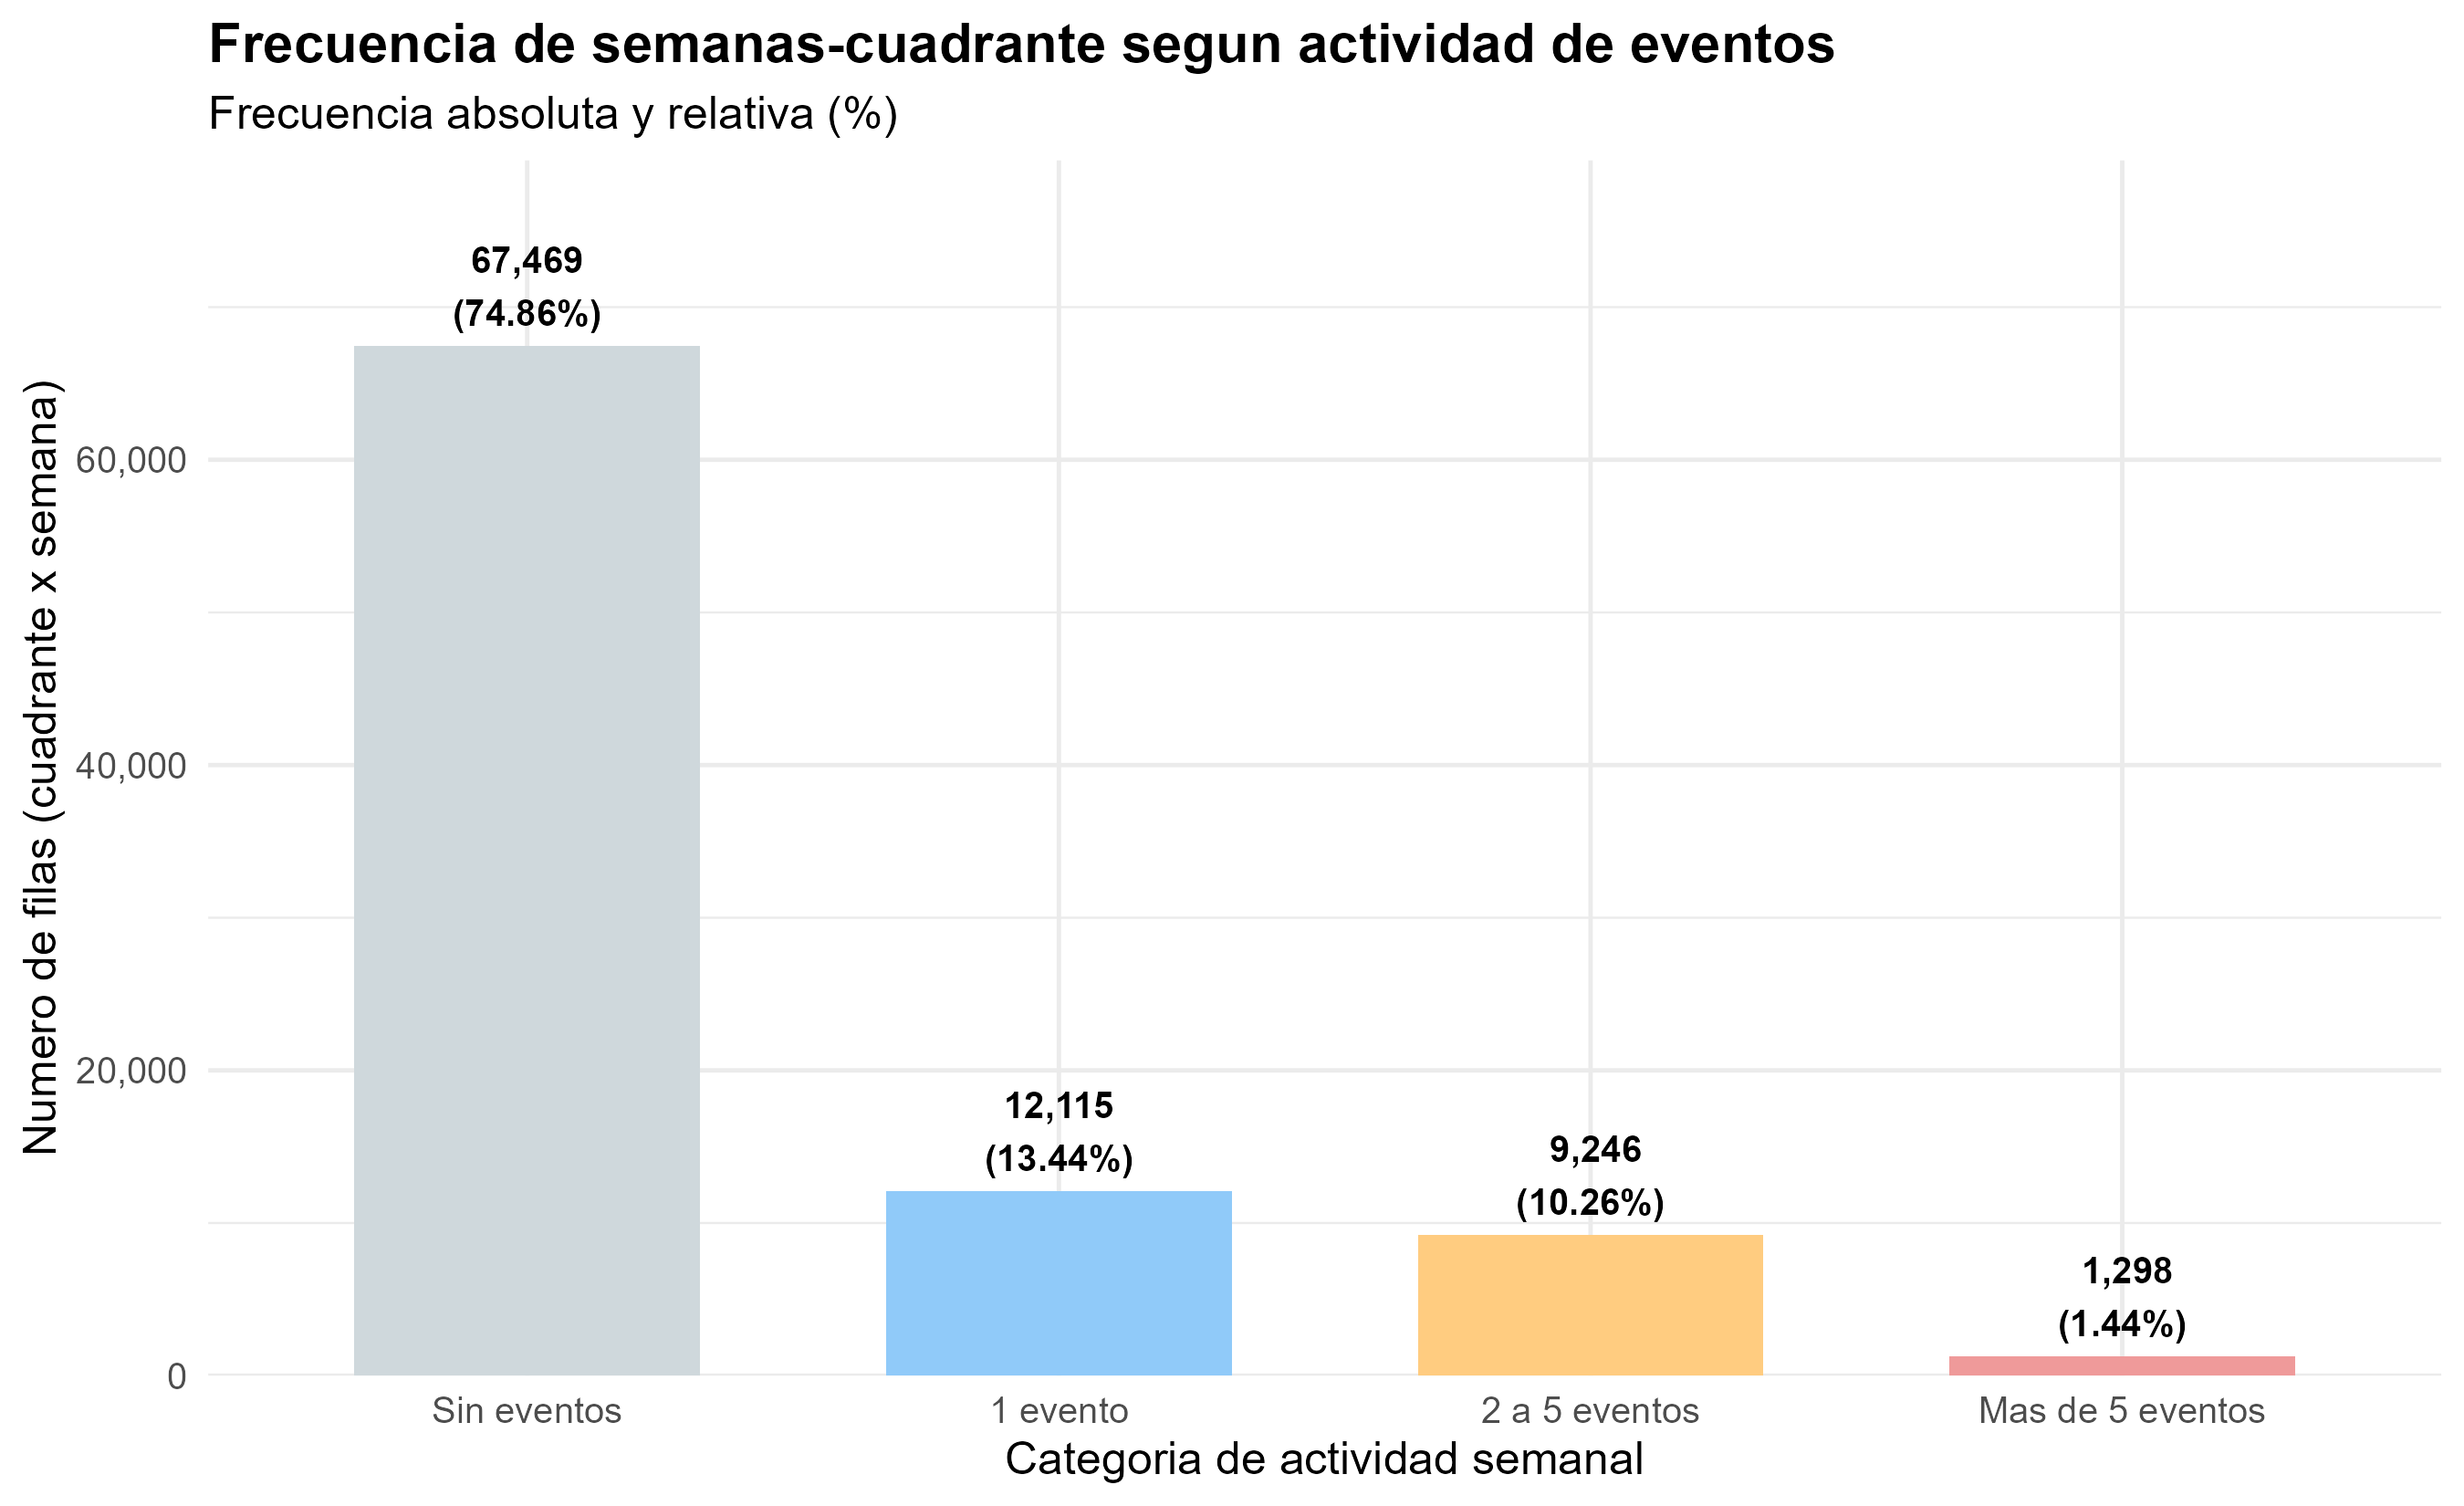
\includegraphics[width=0.85\textwidth]{img/grafico_barras_actividad_agrupada.png}
        \caption{Frecuencia de semanas-cuadrante según actividad de eventos ($N_{\mathrm{agr}} = 90\,128$).}
        \label{fig:barras_actividad_agrupada}
    \end{figure}
    
    \begin{figure}[!htbp]
        \centering
        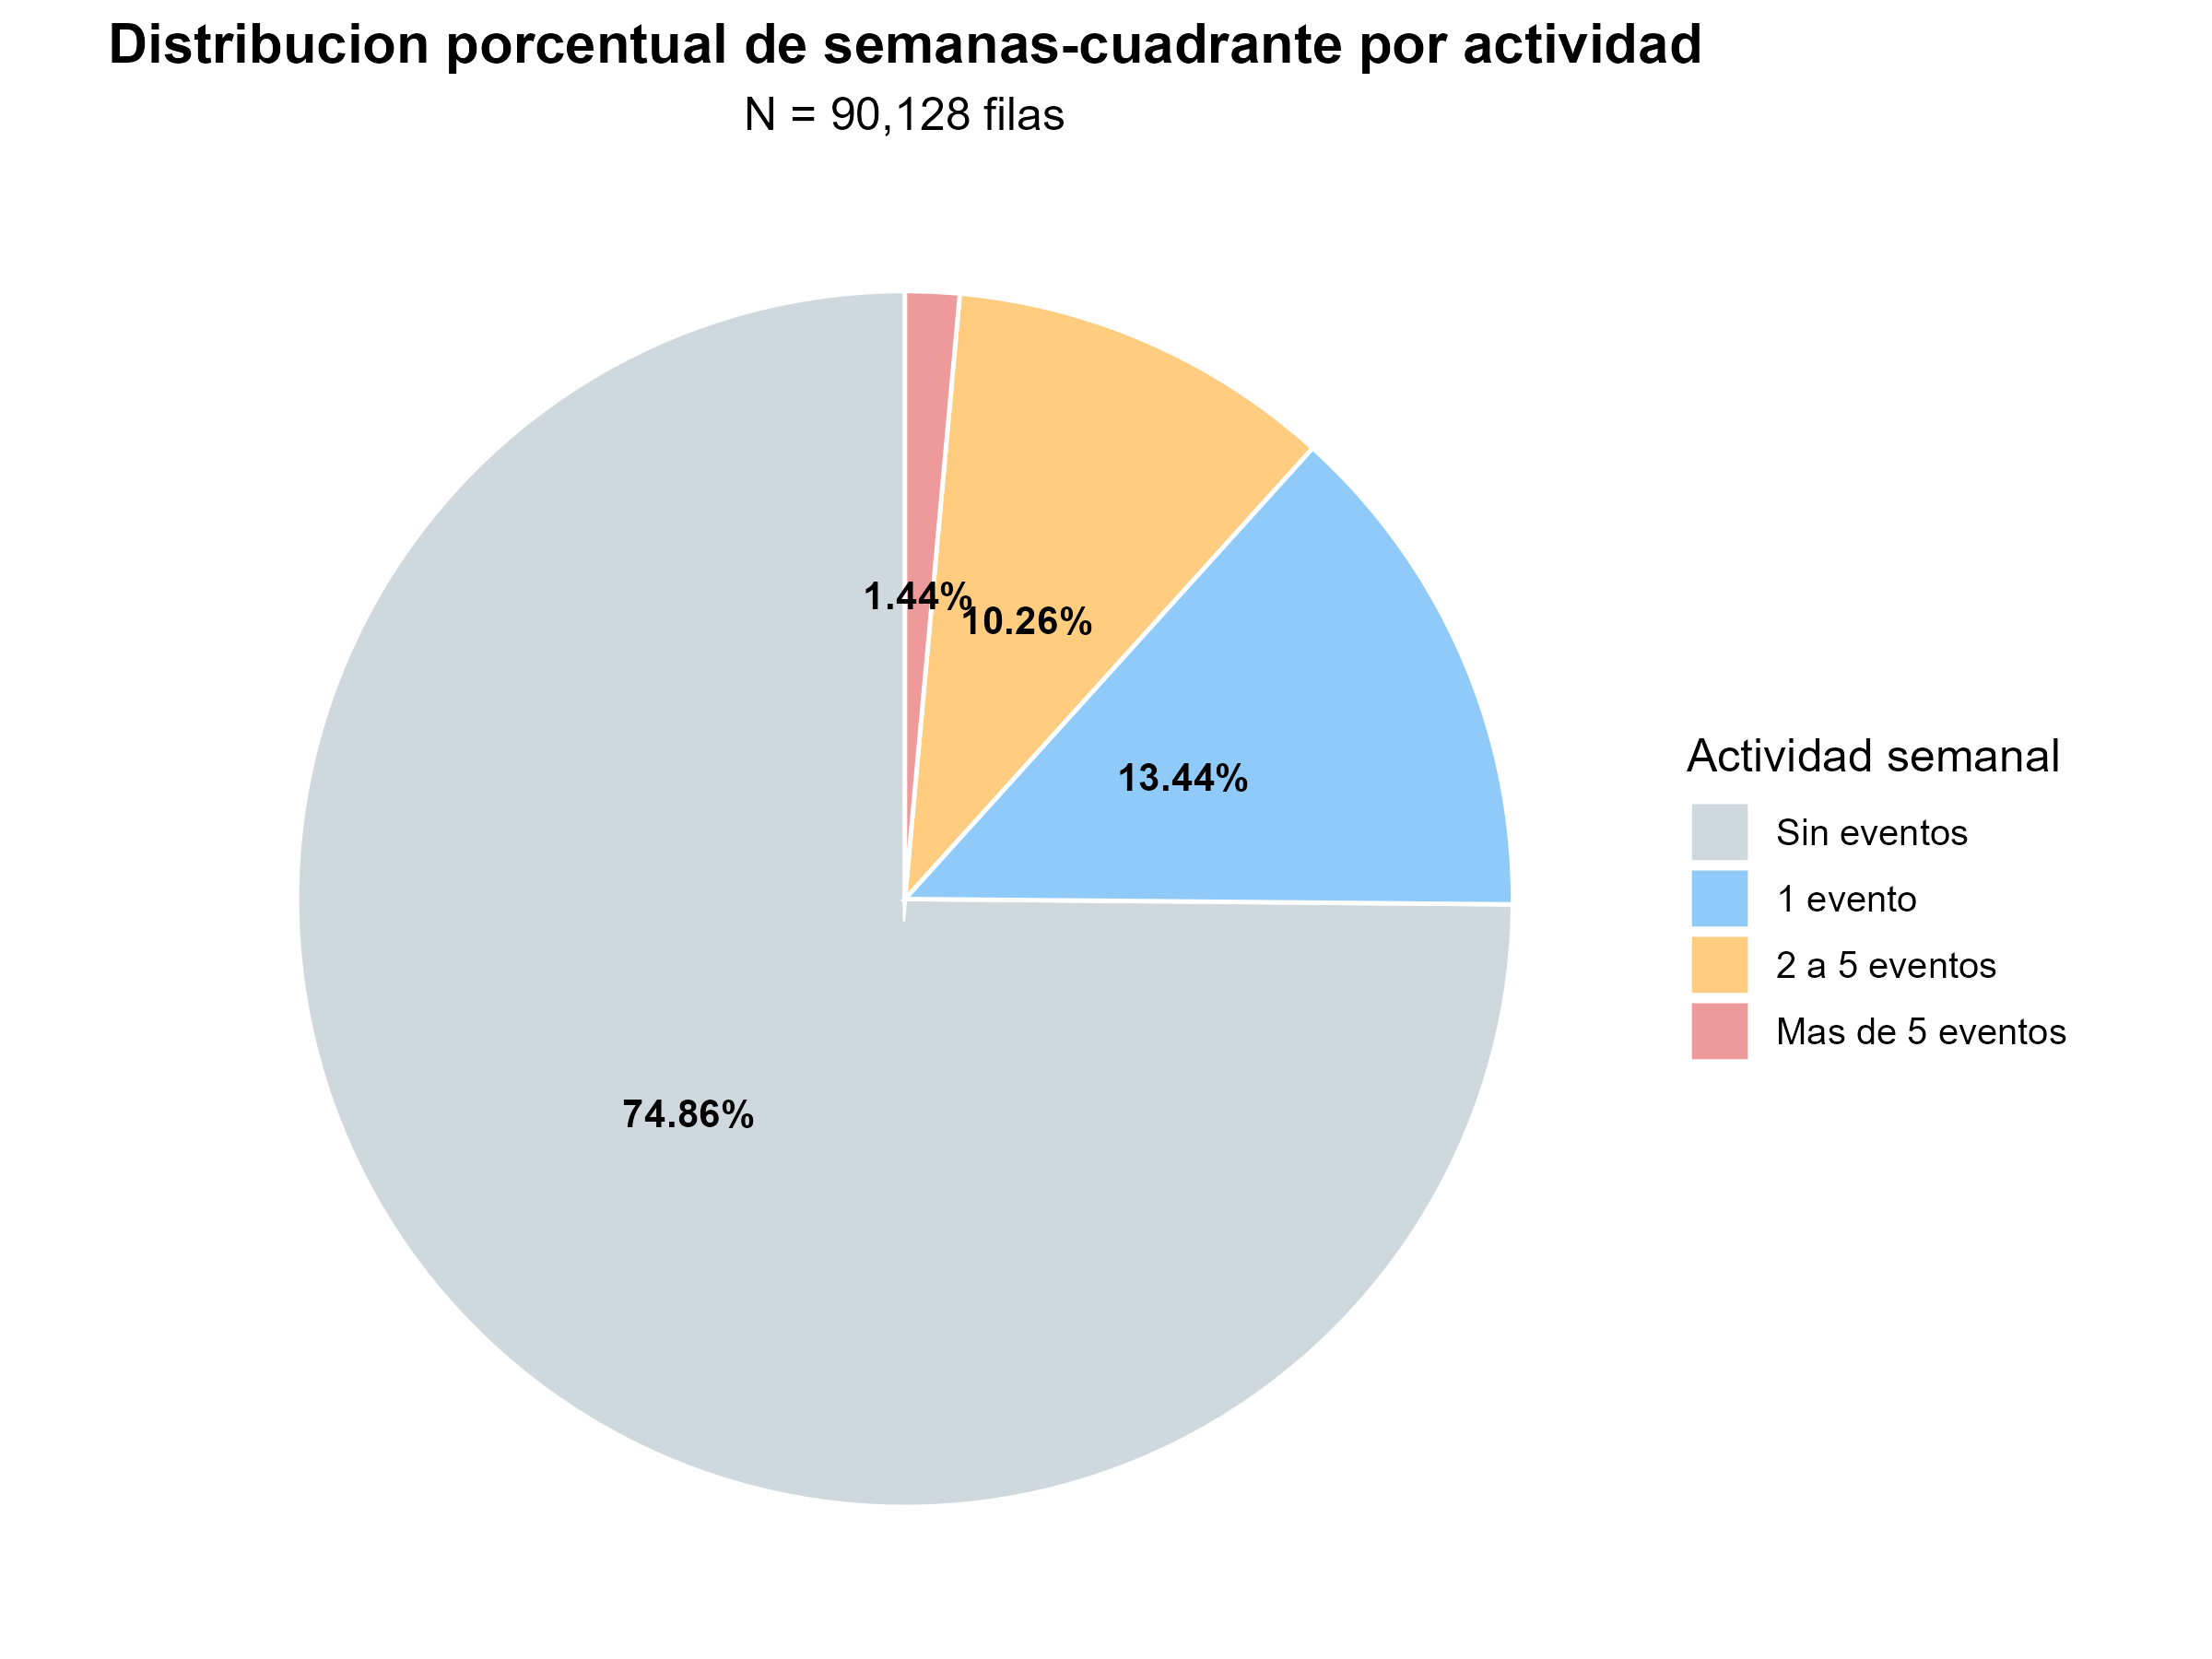
\includegraphics[width=0.70\textwidth]{img/grafico_pastel_actividad_agrupada.png}
        \caption{Distribución porcentual de semanas-cuadrante por actividad de eventos.}
        \label{fig:pastel_actividad_agrupada}
    \end{figure}
    
    \begin{figure}[!htbp]
        \centering
        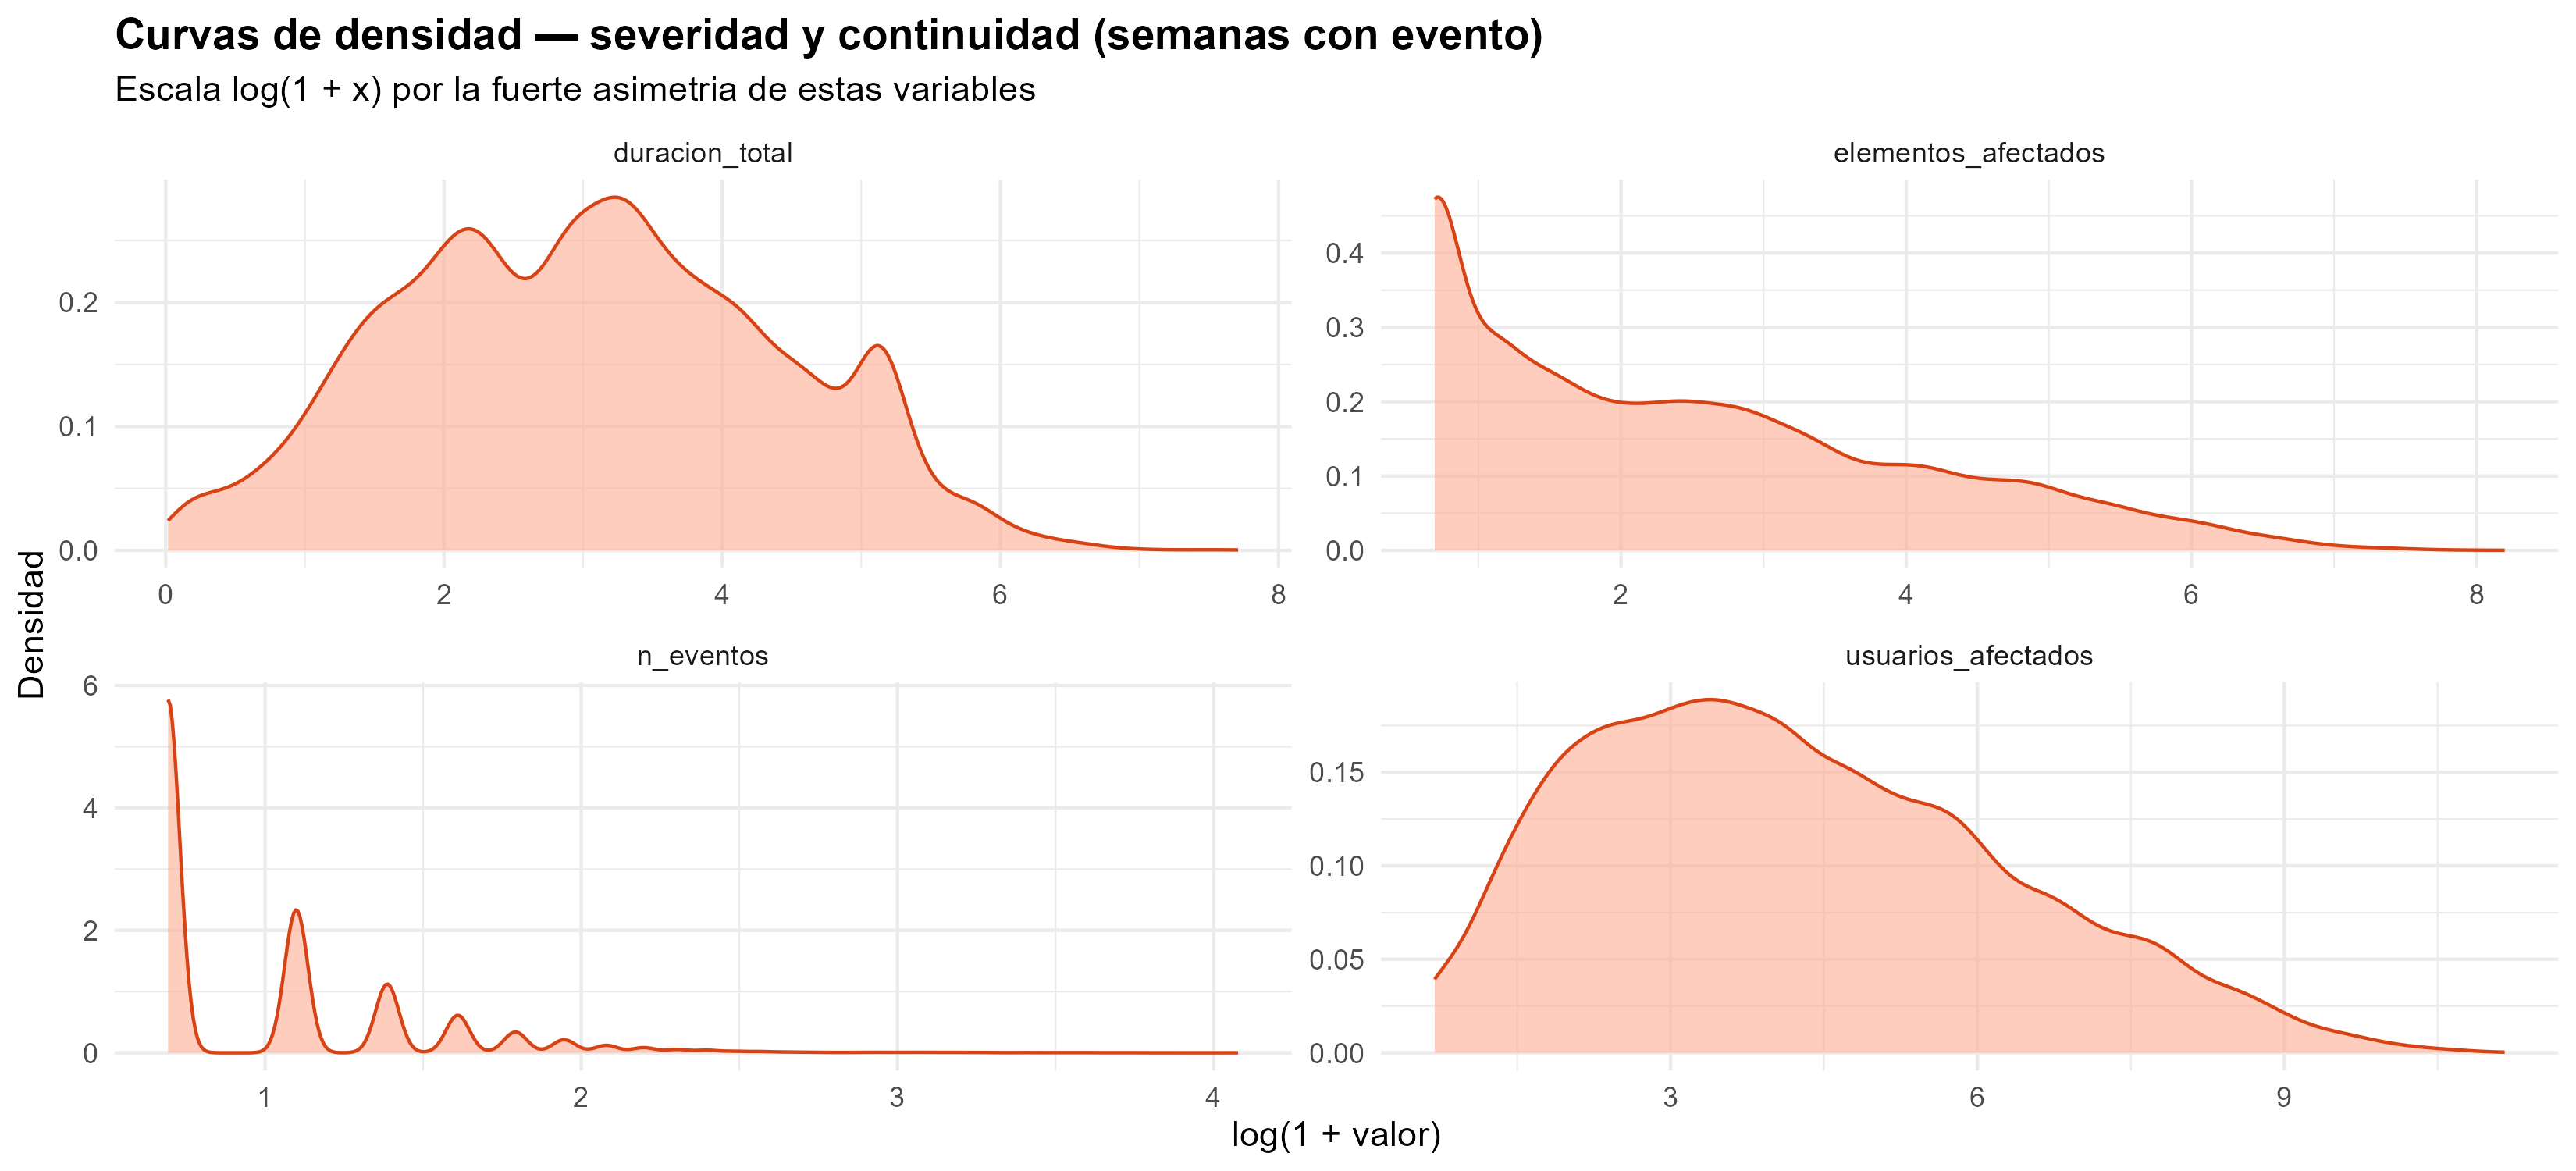
\includegraphics[width=0.95\textwidth]{img/curvas_densidad_evento_agrupada.png}
        \caption{Distribución de la severidad y continuidad en escala logarítmica desplazada (semanas con evento).}
        \label{fig:densidad_evento_agrupada}
    \end{figure}
    
    \noindent En síntesis, el clima semanal exhibe comportamiento estable y casi simétrico, mientras que las variables operativas reflejan fuerte cero-inflación y colas pesadas propias del fenómeno de interrupciones. Estos perfiles, especialmente la asimetría de \texttt{precip\_total\_semana} y la concentración de semanas sin evento, orientan las transformaciones logarítmicas desplazadas (Sección~\ref{sec:metodos-modelos}) y la selección de modelos en la Etapa~4.

\subsection{Análisis de la distribución de variables}
\label{sec:distribucion_variables}
    Con el propósito de comprender el comportamiento estadístico de las variables incluidas en el estudio, se realizó un análisis de distribución sobre las variables climáticas, de severidad y de continuidad contenidas en la tabla agregada cuadrante~$\times$~semana ($N_{\mathrm{agr}} = 90\,128$; Sección~\ref{sec:agrupacion_cuadrante_semana}). Para las variables cuantitativas se emplearon diagramas de densidad, complementados con indicadores de forma (asimetría, curtosis y proporción de ceros) y con el coeficiente de variación reportado en las Secciones~\ref{sec:identificacion_valores_extremos}--\ref{sec:estadisticos_descriptivos}, lo que permitió evaluar simetría, dispersión relativa, unimodalidad y presencia de valores extremos. El procedimiento reproducible se documenta en el Apéndice~\ref{app:html-distribucion}.
    
    \paragraph{Variables climáticas.} Los resultados evidencian que las variables meteorológicas presentan distribuciones heterogéneas. Las temperaturas (media, máxima y mínima) y la humedad relativa muestran comportamientos estables, aproximadamente unimodales, con asimetría cercana a cero (entre $-0{.}49$ y $-0{.}36$) y CV bajo ($0{.}16$--$0{.}25$), coherentes con las curvas de densidad presentadas en la Figura~\ref{fig:densidad_clima_agrupada}. En contraste, la precipitación acumulada semanal presenta asimetría positiva (coeficiente de $1{.}98$ y curtosis con exceso de $4{.}78$), CV $= 1{.}17$, alta frecuencia de semanas con valores bajos de lluvia (el $9{.}1$~\% registra $0$~mm) y un número reducido de observaciones con precipitaciones intensas. La Figura~\ref{fig:densidad_precipitacion_agrupada} contrasta la distribución en escala original y en escala logarítmica desplazada (Sección~\ref{sec:metodos-modelos}): la transformación aproxima la distribución a una forma simétrica, lo que anticipa su utilidad en la Etapa~4.
    
    \begin{figure}[!htbp]
        \centering
        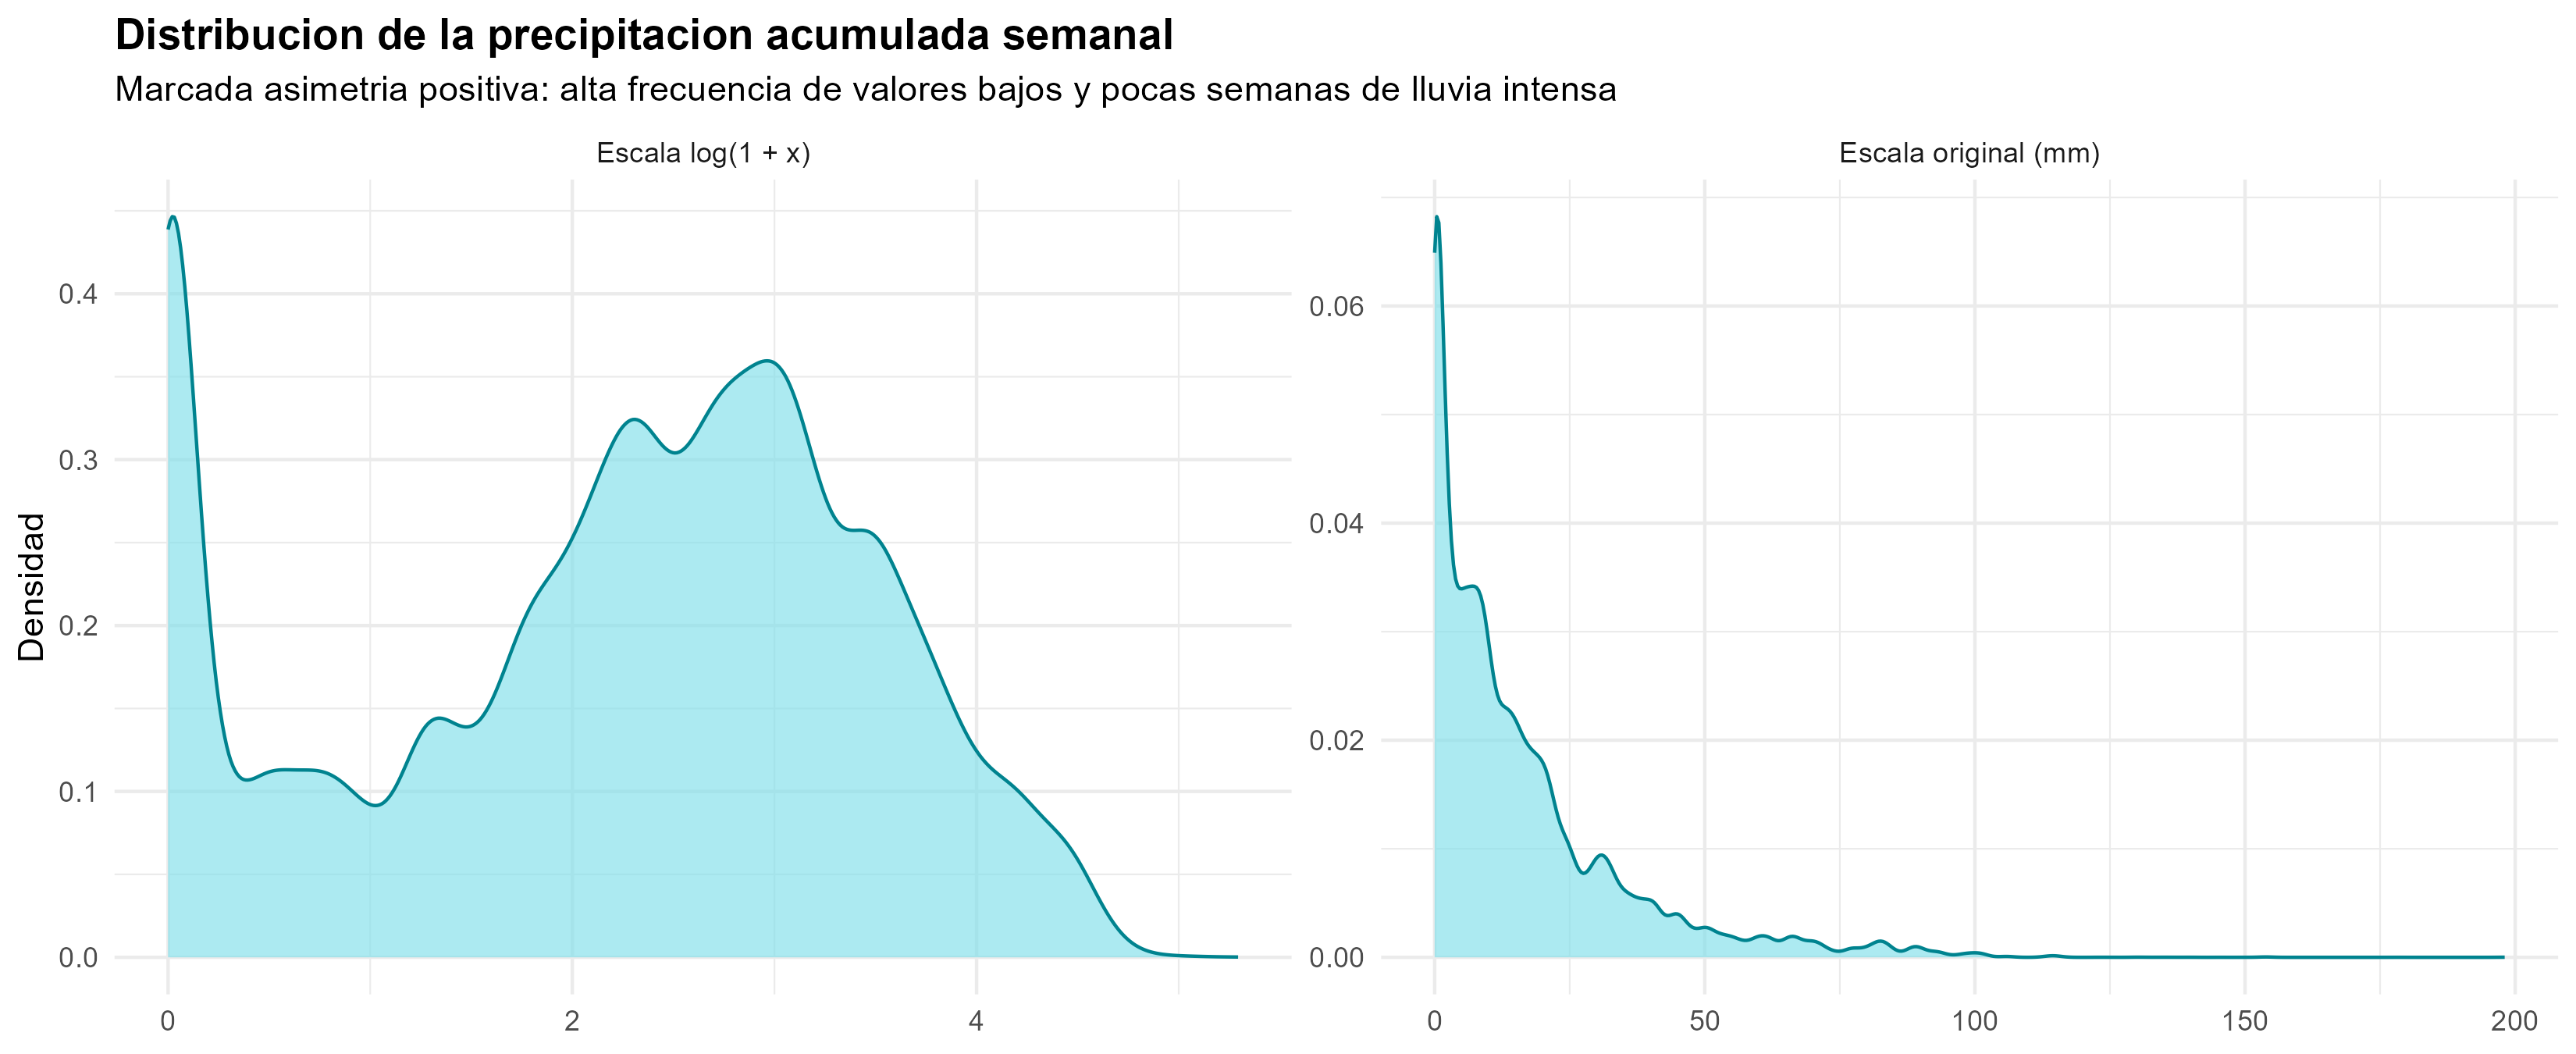
\includegraphics[width=0.95\textwidth]{img/distribucion_densidad_precipitacion_agrupada.png}
        \caption{Distribución de la precipitación acumulada semanal en escala original y logarítmica desplazada ($N_{\mathrm{agr}} = 90\,128$).}
        \label{fig:densidad_precipitacion_agrupada}
    \end{figure}
    
    \paragraph{Variables de severidad y continuidad.} Las variables asociadas a interrupciones del servicio (\texttt{usuarios\_afectados}, \texttt{elementos\_afectados}, \texttt{duracion\_total} y \texttt{n\_eventos}) muestran distribuciones altamente sesgadas hacia cero: la proporción de filas con valor $0$ se ubica entre el $72{.}5$~\% (\texttt{duracion\_total}) y el $74{.}9$~\% (resto de variables), como ilustra la Figura~\ref{fig:pct_ceros_evento_agrupada}. Este comportamiento es esperado, dado que la mayor parte de las semanas-cuadrante no registra fallas. Sin embargo, condicionando a la ocurrencia de eventos ($\text{valor} > 0$), las distribuciones presentan colas derechas largas, con asimetrías entre $8{.}2$ y $20{.}6$ y curtosis entre $139$ y $643$, que reflejan la existencia de incidentes de alta severidad con impacto significativo sobre la continuidad del servicio, según se aprecia en las densidades en escala logarítmica desplazada de la Figura~\ref{fig:densidad_evento_agrupada}.
    
    \begin{figure}[!htbp]
        \centering
        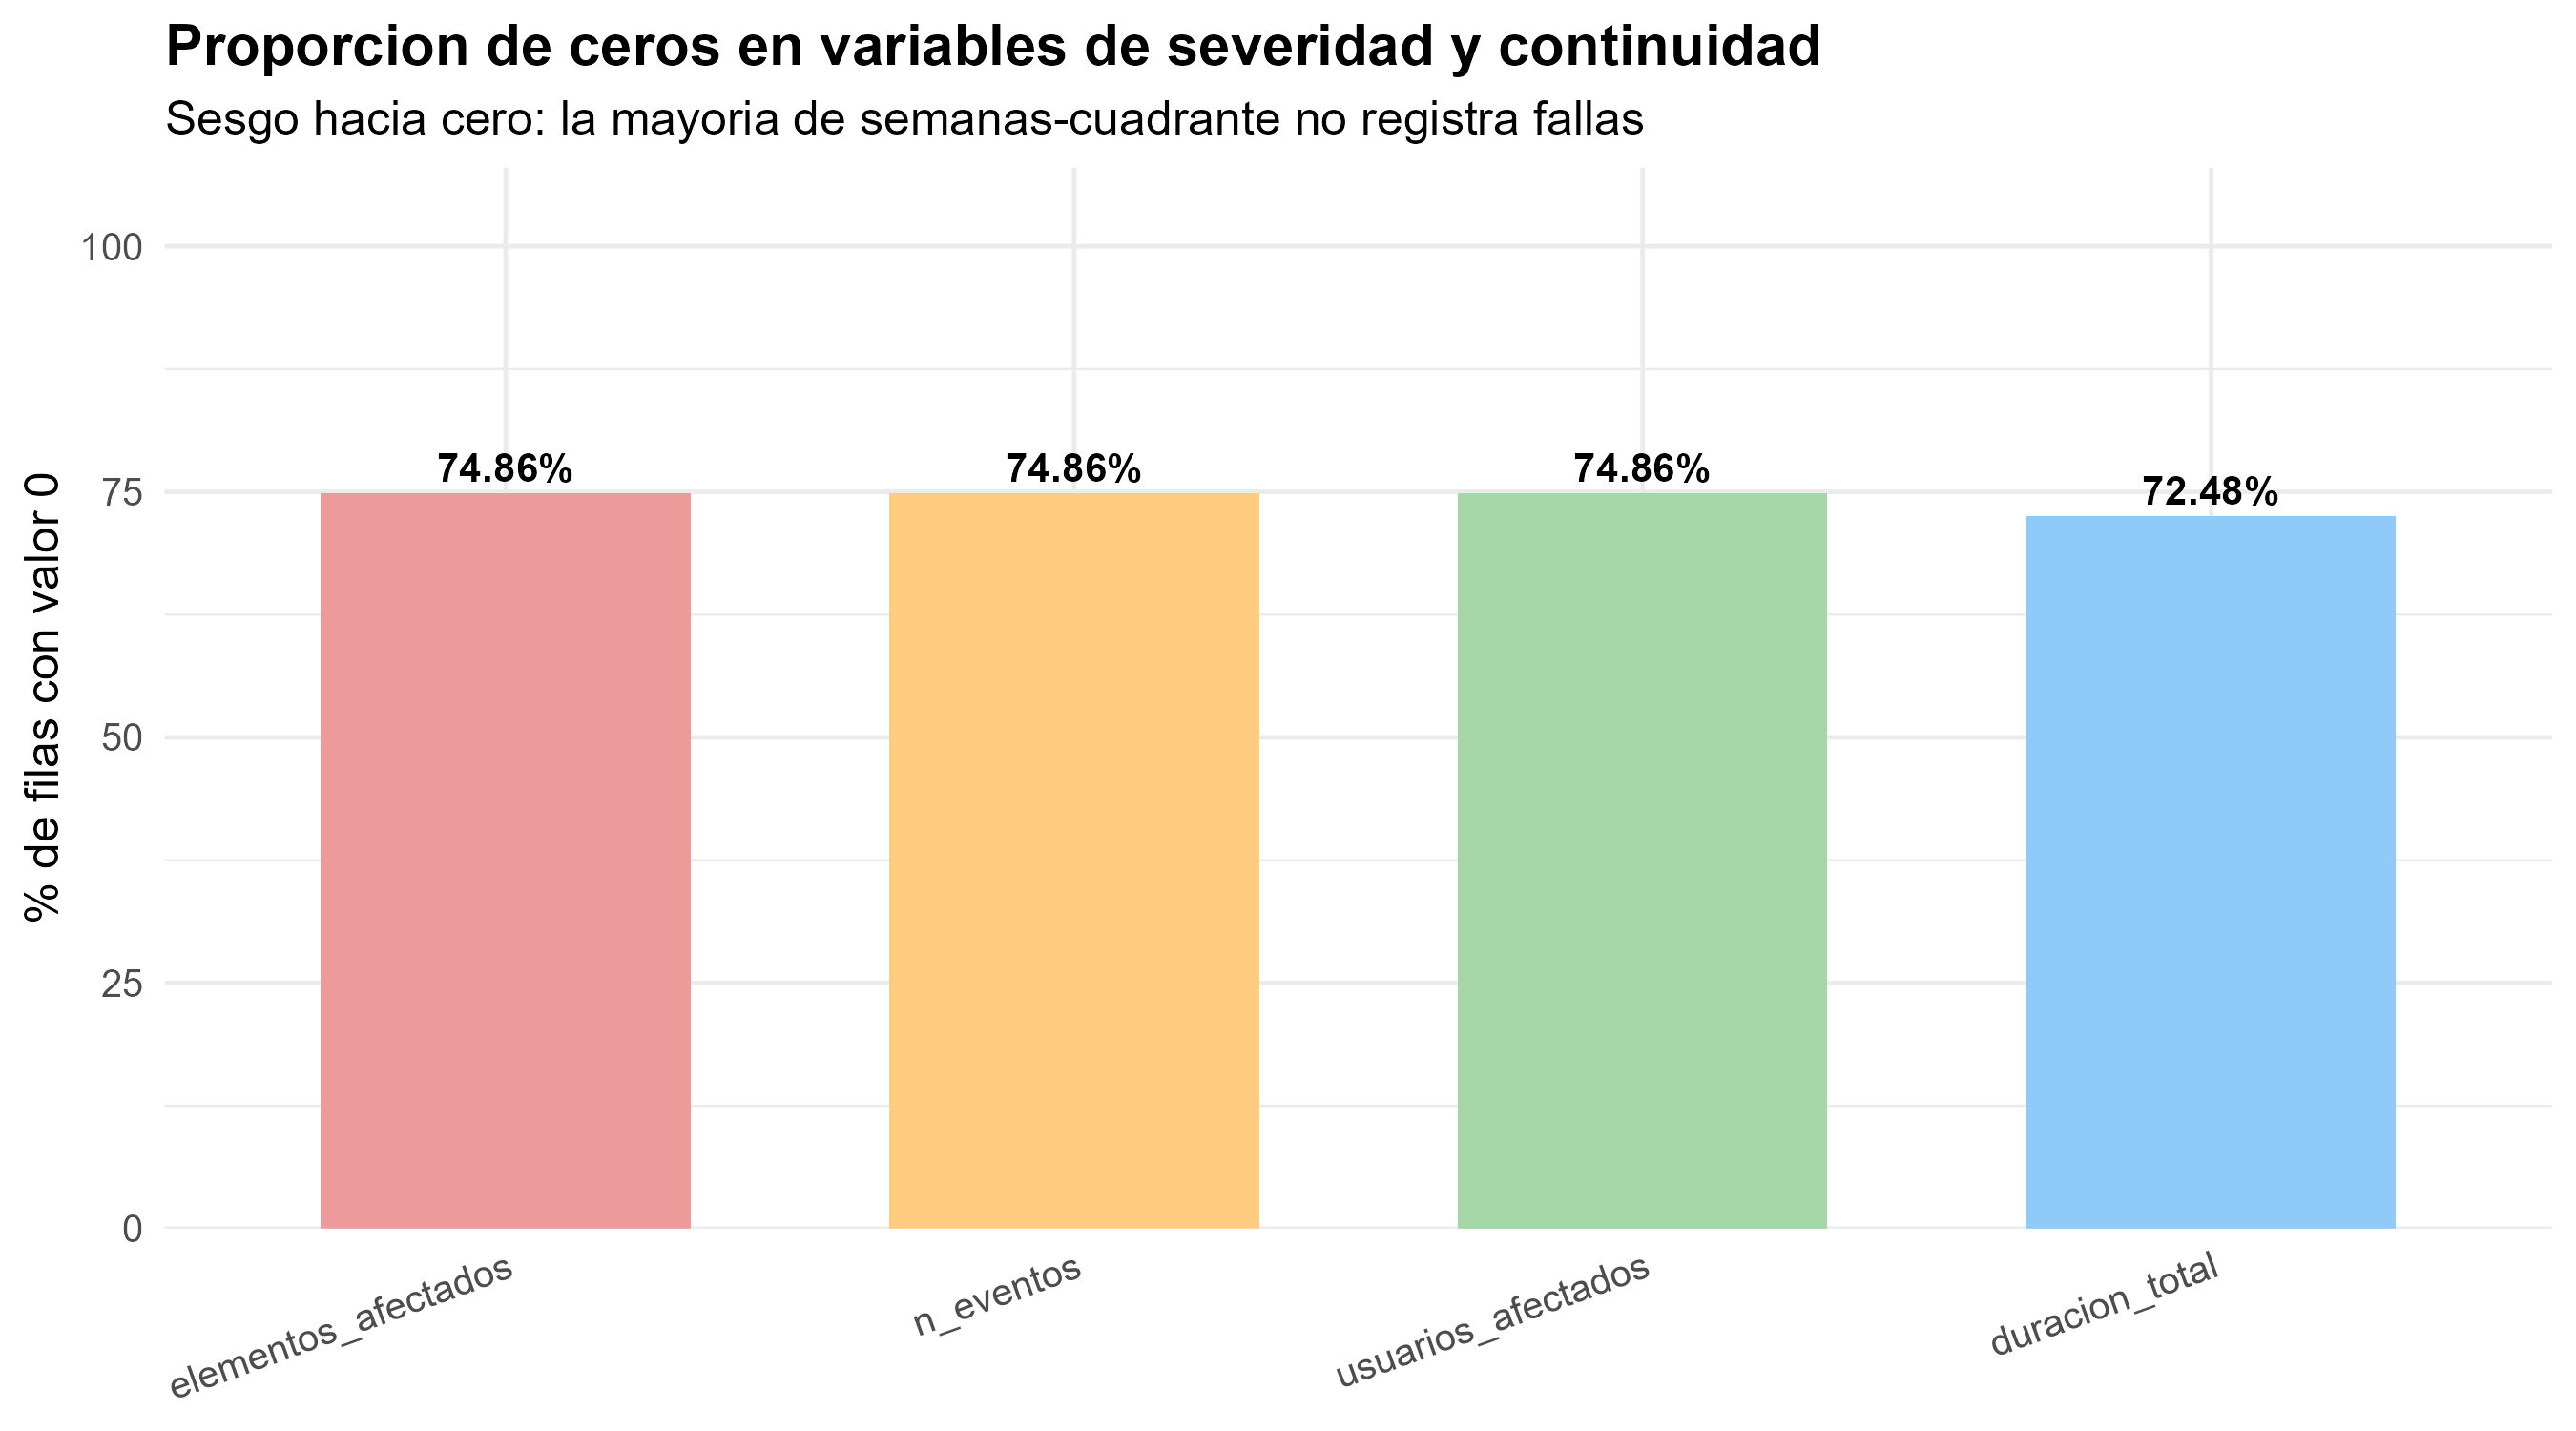
\includegraphics[width=0.85\textwidth]{img/distribucion_pct_ceros_evento_agrupada.png}
        \caption{Proporción de ceros en las variables de severidad y continuidad de la tabla agrupada.}
        \label{fig:pct_ceros_evento_agrupada}
    \end{figure}
    
    \noindent En síntesis, el análisis de distribución confirma dos regímenes claramente diferenciados: un bloque climático estable y casi simétrico (CV bajo, con la precipitación como excepción asimétrica de CV algo superior a la unidad) y un bloque operativo cero-inflado con colas pesadas y CV condicionado alto. Estos hallazgos fundamentan las transformaciones logarítmicas desplazadas (Sección~\ref{sec:metodos-modelos}) y la consideración de modelos aptos para datos cero-inflados en la Etapa~4.
    
\subsection{Análisis temporal de eventos}
\label{sec:analisis_temporal_eventos}
    Para caracterizar la dinámica temporal de las interrupciones se construyó, a partir de la tabla agregada \texttt{data\_agrupada.csv} (Sección~\ref{sec:agrupacion_cuadrante_semana}), la serie territorial semanal que consolida el total de \texttt{n\_eventos} de todos los cuadrantes en cada semana calendario. La serie cubre $262$ semanas del horizonte 2021--2025, con una mediana de $124{.}5$ eventos por semana (media $188{.}5$; máximo $648$). El procedimiento reproducible se documenta en el Apéndice~\ref{app:html-temporal}.
    
    \paragraph{Evolución de la serie semanal.} La Figura~\ref{fig:serie_semanal_eventos} presenta la serie semanal con su tendencia suavizada (LOESS) sobre el horizonte exploratorio 2021--2025 ($D_{\mathrm{EDA}}$). Se distinguen dos regímenes visuales: entre 2021 y 2023 la actividad se mantiene en un nivel bajo y relativamente estable, mientras que a partir de 2024 se observa un incremento sostenido del nivel de la serie. La agregación anual (Figura~\ref{fig:eventos_por_anio}) cuantifica este cambio: de $5\,167$ eventos en 2021 y $4\,934$ en 2022, se pasa a $15\,211$ en 2024 y $18\,199$ en 2025; en términos de intensidad, el promedio asciende de $\approx 99$ a $\approx 350$ eventos por semana entre 2021 y 2025. La reinterpretación de este salto a la luz de la cobertura de integración se desarrolla en el párrafo siguiente (Sección~\ref{sec:delimitacion_temporal_modelado}).
    
    \begin{figure}[!htbp]
        \centering
        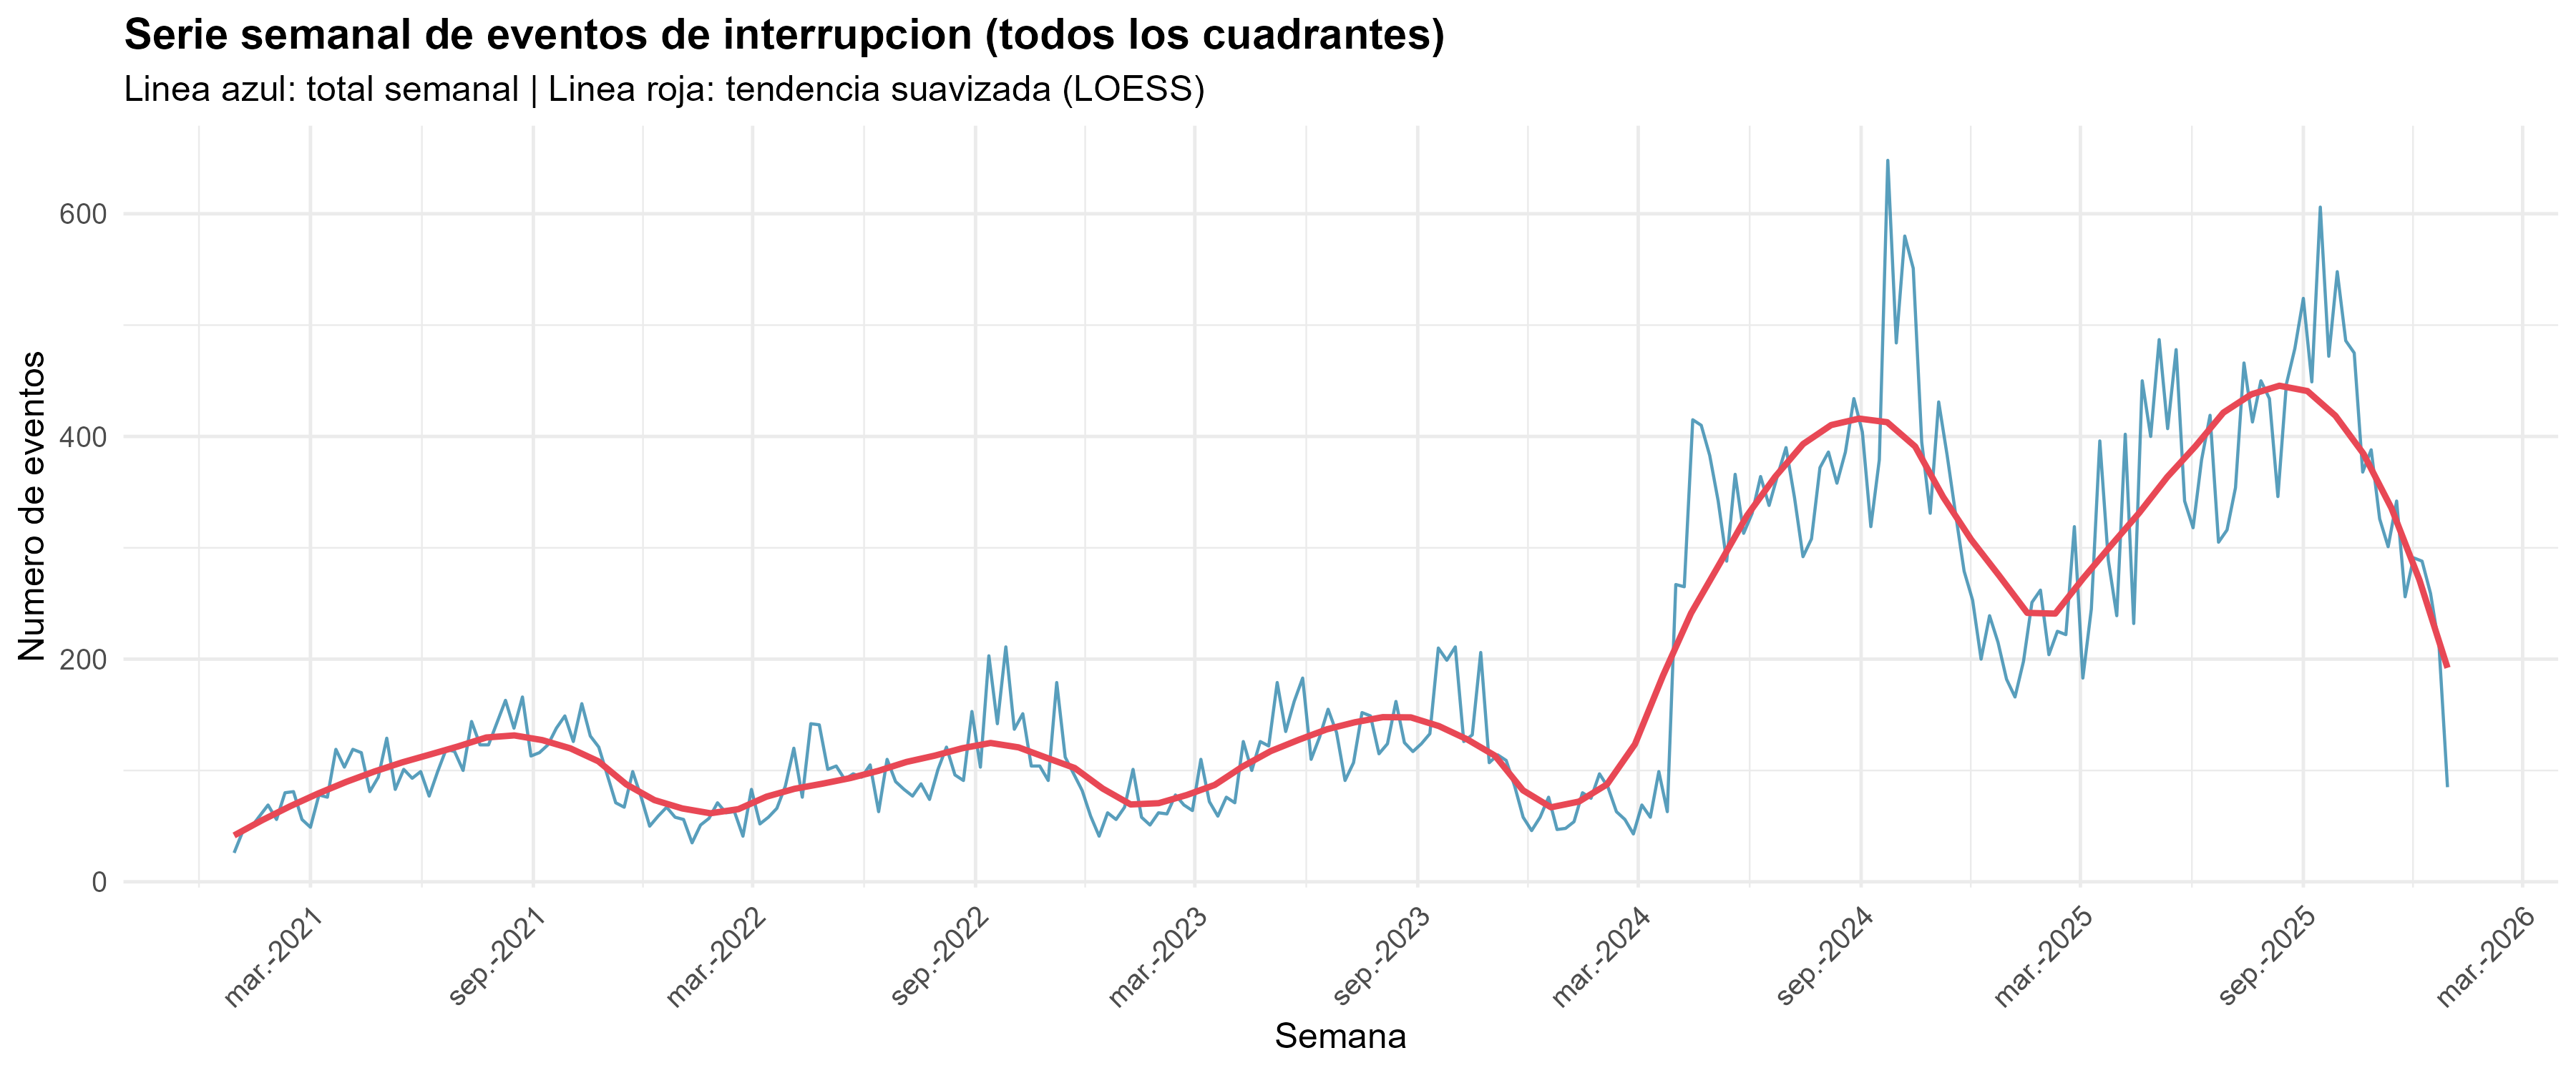
\includegraphics[width=0.95\textwidth]{img/serie_semanal_eventos_agrupada.png}
        \caption{Evolución semanal de los eventos de interrupción (suma territorial), 2021--2025.}
        \label{fig:serie_semanal_eventos}
    \end{figure}
    
    \begin{figure}[!htbp]
        \centering
        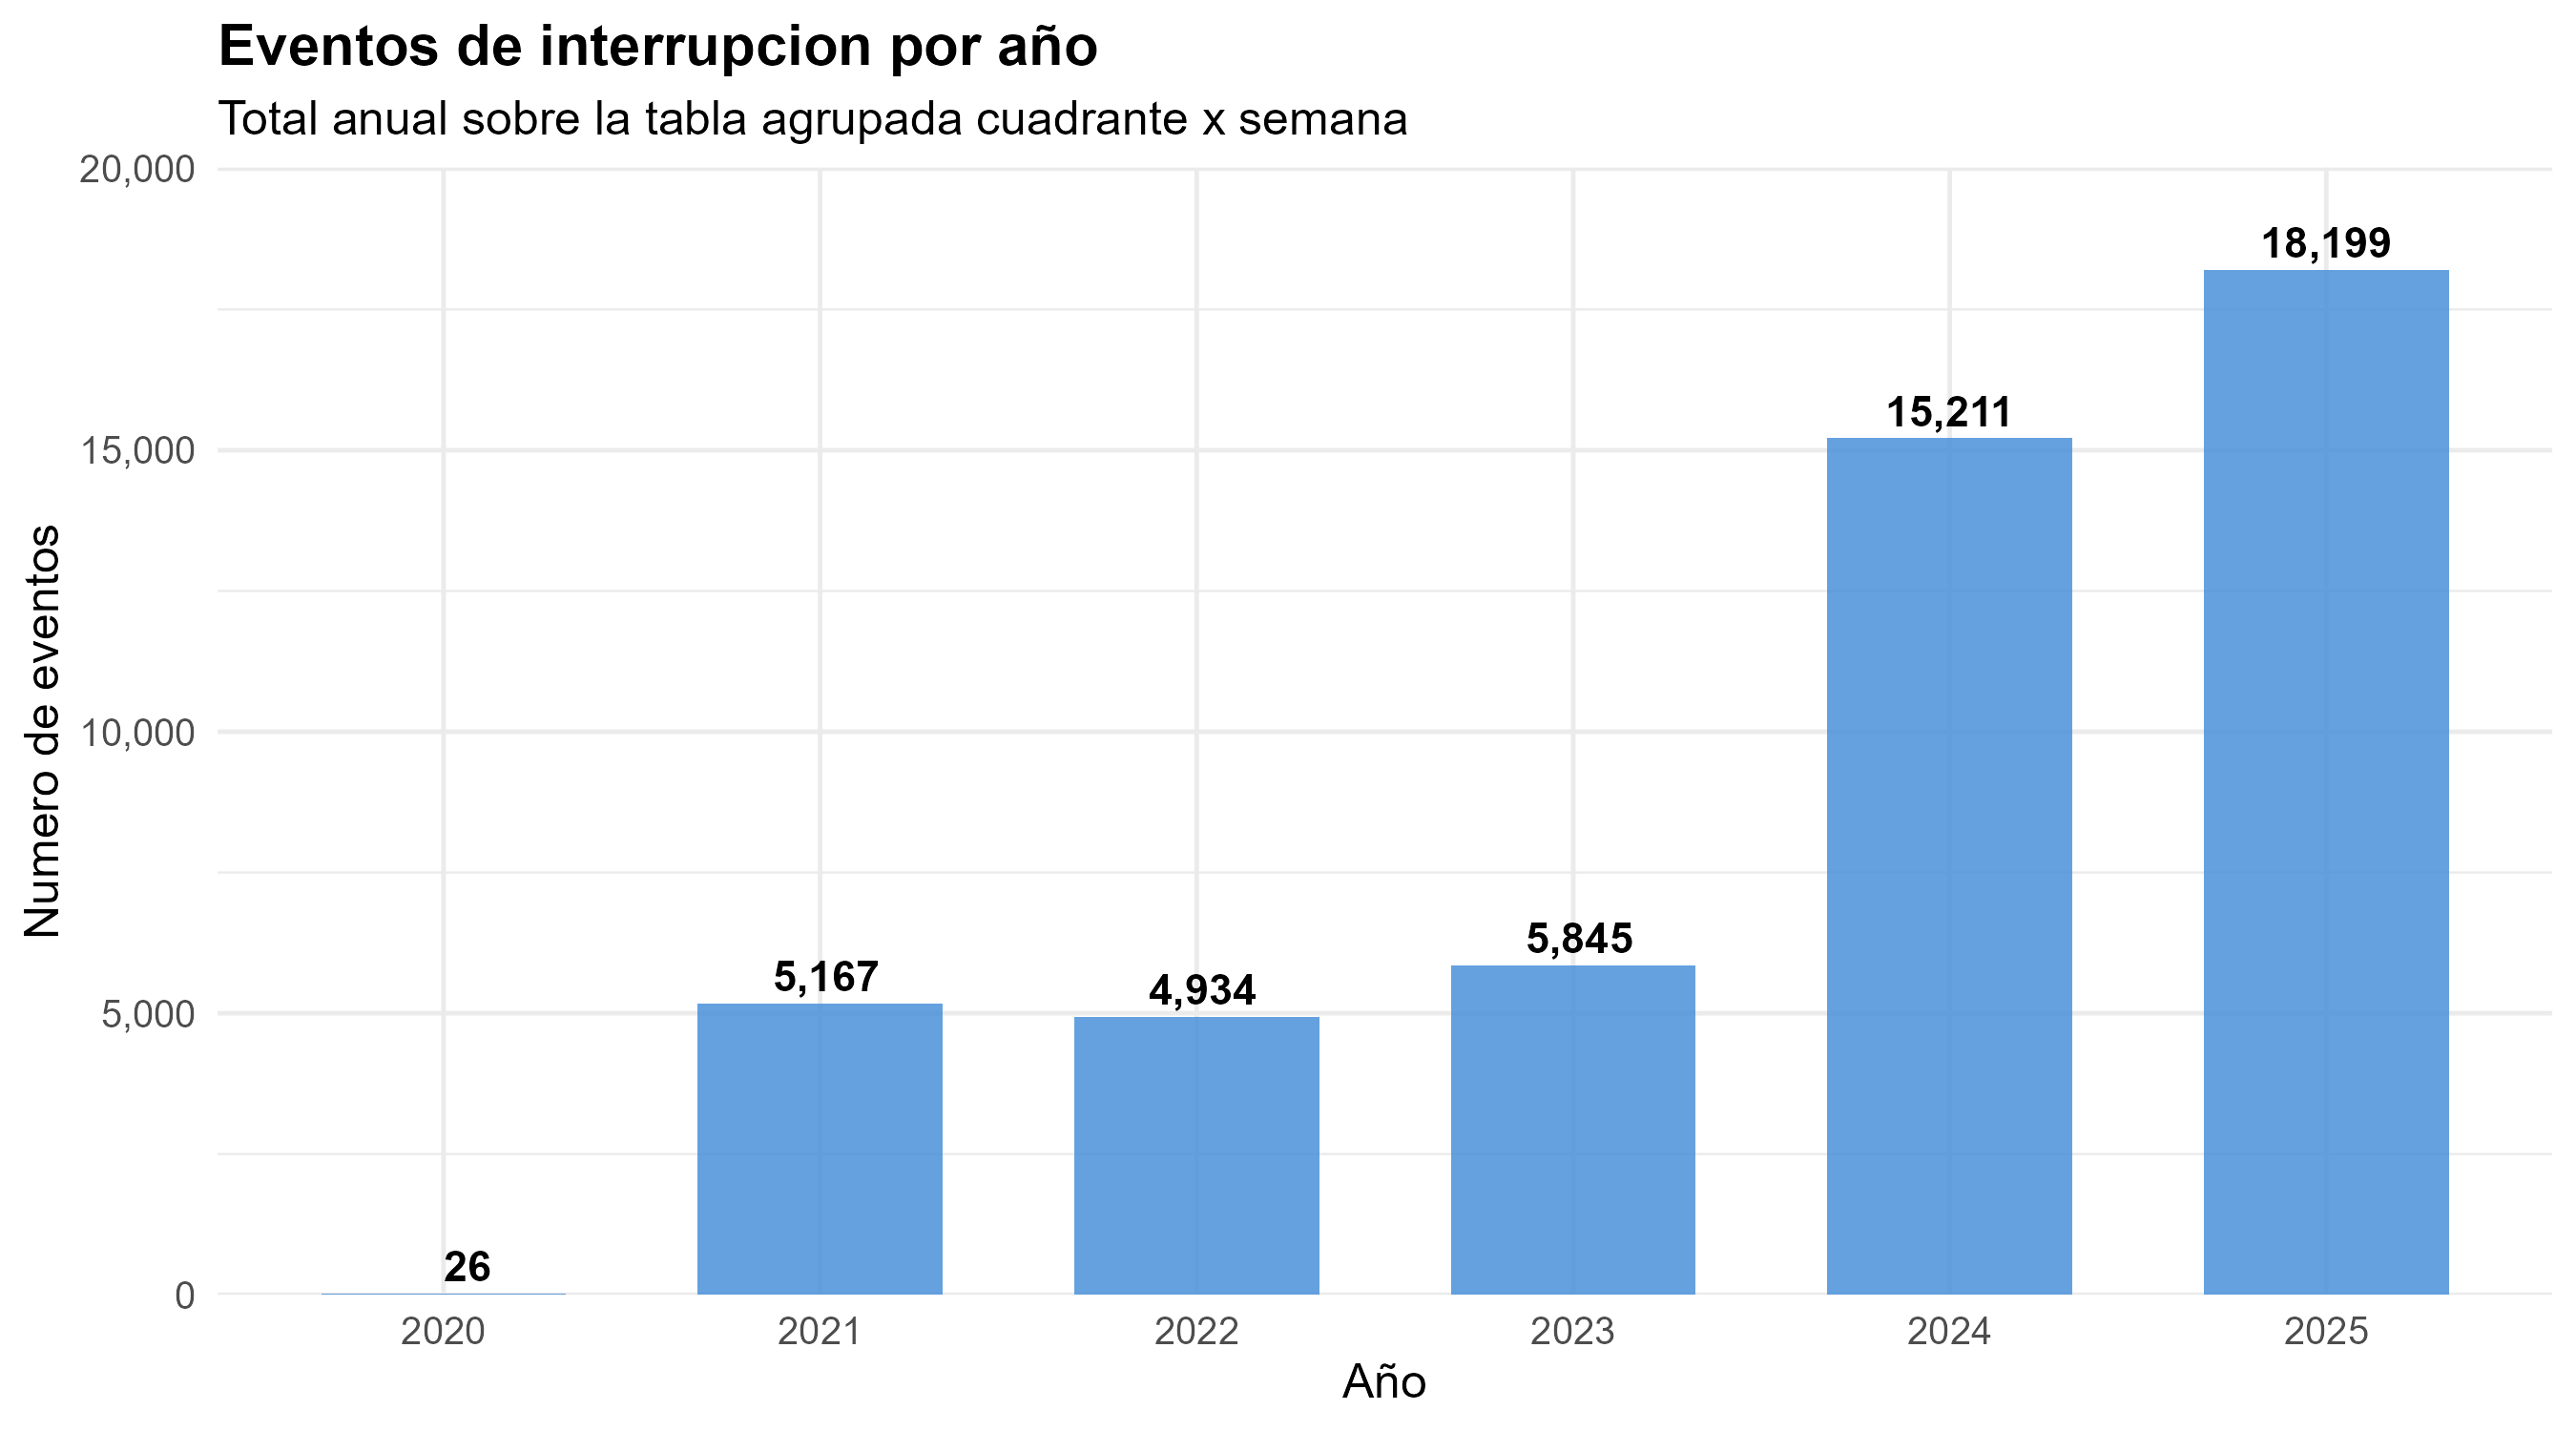
\includegraphics[width=0.80\textwidth]{img/eventos_por_anio_agrupada.png}
        \caption{Total anual de eventos de interrupción sobre la tabla agrupada.}
        \label{fig:eventos_por_anio}
    \end{figure}
    
    \paragraph{Diagnóstico de cobertura del emparejamiento evento--elemento.}
    \label{sec:delimitacion_temporal_modelado}
    
    Al contrastar el conteo anual de eventos en \texttt{tabla\_eventos\_ajustado.csv} (BRAE) con la suma territorial de \texttt{n\_eventos} en \texttt{data\_agrupada.csv}, se identificó un \textit{sesgo sistemático} en el grano espacial durante 2021--2023 (Tabla~\ref{tab:cobertura_emparejamiento_oms}; Figura~\ref{fig:cobertura_emparejamiento}). La causa no es la ausencia del campo \texttt{COMPONENTE\_FALLADO}, completo en el $100$~\% de los registros BRAE, sino la \textit{incompatibilidad entre esquemas de codificación} al cruzar eventos con el inventario georreferenciado \texttt{tipo\_elemento.csv} (Tabla~\ref{tab:muestra_inventario_gis}).
    
    En la operación de la red coexisten dos identificadores para un mismo punto de conexión: (i)~el \textit{código de sitio} (ubicación), estable en el tiempo y empleado por el inventario GIS como \texttt{ELEMENTO}; y (ii)~el \textit{código de activo}, asociado al equipo instalado y \textit{sujeto a cambio} cuando el activo se repone por mantenimiento o renovación, mientras el código de sitio permanece invariante. El panel consolidado y la agregación cuadrante~$\times$~semana se construyen sobre el código de sitio. No obstante, en el sistema histórico OMS-SPARD (Sección~\ref{sec:extraccion_oms_historico}) el elemento fallado (\texttt{BREAKER} $\rightarrow$ \texttt{COMPONENTE\_FALLADO}) se registraba con frecuencia mediante el \textit{código del activo} y no el del sitio. Ello impide el seguimiento histórico del punto de desconexión, unidad espacial central para el pronóstico territorial de $SAIDI$ y $SAIFI$ en esta tesis, pues el cruce \texttt{COMPONENTE\_FALLADO} $=$ \texttt{ELEMENTO} no encuentra coincidencia en el inventario y el evento no genera \texttt{FRECUENCIA} en el panel activo~$\times$~día.
    
    El diagnóstico cuantitativo confirma esta hipótesis: la proporción de eventos cuyo \texttt{COMPONENTE\_FALLADO} coincide con algún \texttt{ELEMENTO} de \texttt{tipo\_elemento.csv} es del $30{.}5$~\% (2021), $30{.}9$~\% (2022) y $31{.}7$~\% (2023), valores cercanos a la cobertura del panel espacial en esos años ($28{.}1$~\%, $28{.}1$~\% y $29{.}1$~\%, respectivamente). Con la migración a OMS-SP7 (Sección~\ref{sec:extraccion_oms_actual}), la coincidencia asciende al $79{.}8$~\% (2024) y al $95{.}0$~\% (2025), acompañada por coberturas del panel del $77{.}7$~\% y $92{.}4$~\%. La Figura~\ref{fig:eventos_por_anio} debe interpretarse a la luz de esta brecha: el salto a partir de 2024 refleja en gran medida una \textit{mayor homogeneización de la codificación} bajo OMS-SP7, y no únicamente un incremento operativo de interrupciones.
    
    El procedimiento reproducible se documenta en el Apéndice~\ref{app:html-emparejamiento}. Con base en este hallazgo, emergido en el presente análisis temporal, se define el \textit{dataset de modelado} $D_{\mathrm{mod}}$ como el subconjunto de \texttt{data\_agrupada.csv} con \texttt{year(semana)} $\in \{2024,\,2025\}$, que comprende $36\,120$ filas cuadrante~$\times$~semana, $105$ semanas y $33\,410$ eventos georreferenciados en total ($15\,211$ en 2024 y $18\,199$ en 2025). El horizonte 2021--2025 se conserva como $D_{\mathrm{EDA}}$ para las Secciones~\ref{sec:identificacion_datos_faltantes}--\ref{sec:analisis_temporal_eventos}, pero \textit{no} se empleará para estimar el modelo predictivo de la Etapa~4.
    
    \begin{table}[!htbp]
    \centering
\footnotesize
    \setlength{\tabcolsep}{4pt}
    \caption{Cobertura anual de la trazabilidad al inventario GIS y al panel espacial.}
    \label{tab:cobertura_emparejamiento_oms}
    \begin{tabular}{@{}l r r r r@{}}
    \toprule
    \textbf{Año} & \textbf{Eventos BRAE} & \textbf{En inventario (\%)} & \textbf{Panel espacial} & \textbf{Cobertura (\%)} \\
    \midrule
    2021 & 18\,398 & 30.5 & 5\,167  & 28.1 \\
    2022 & 17\,542 & 30.9 & 4\,934  & 28.1 \\
    2023 & 20\,068 & 31.7 & 5\,845  & 29.1 \\
    2024 & 19\,583 & 79.8 & 15\,211 & 77.7 \\
    2025 & 19\,689 & 95.0 & 18\,199 & 92.4 \\
    \bottomrule
    \end{tabular}
    
    \noindent\textit{Nota:} ``En inventario (\%)'' es la proporción de eventos cuyo \texttt{COMPONENTE\_FALLADO} coincide con \texttt{ELEMENTO} en \texttt{tipo\_elemento.csv} (código de sitio). ``Panel espacial'' es la suma anual de \texttt{n\_eventos} en \texttt{data\_agrupada.csv}. La brecha entre ambas columnas en 2021--2023 se atribuye al registro del código de activo, y no del código de sitio, en OMS-SPARD, lo que impide el seguimiento histórico del punto de desconexión. Los años 2024--2025 delimitan $D_{\mathrm{mod}}$.
\end{table}

    \begin{figure}[!htbp]
        \centering
        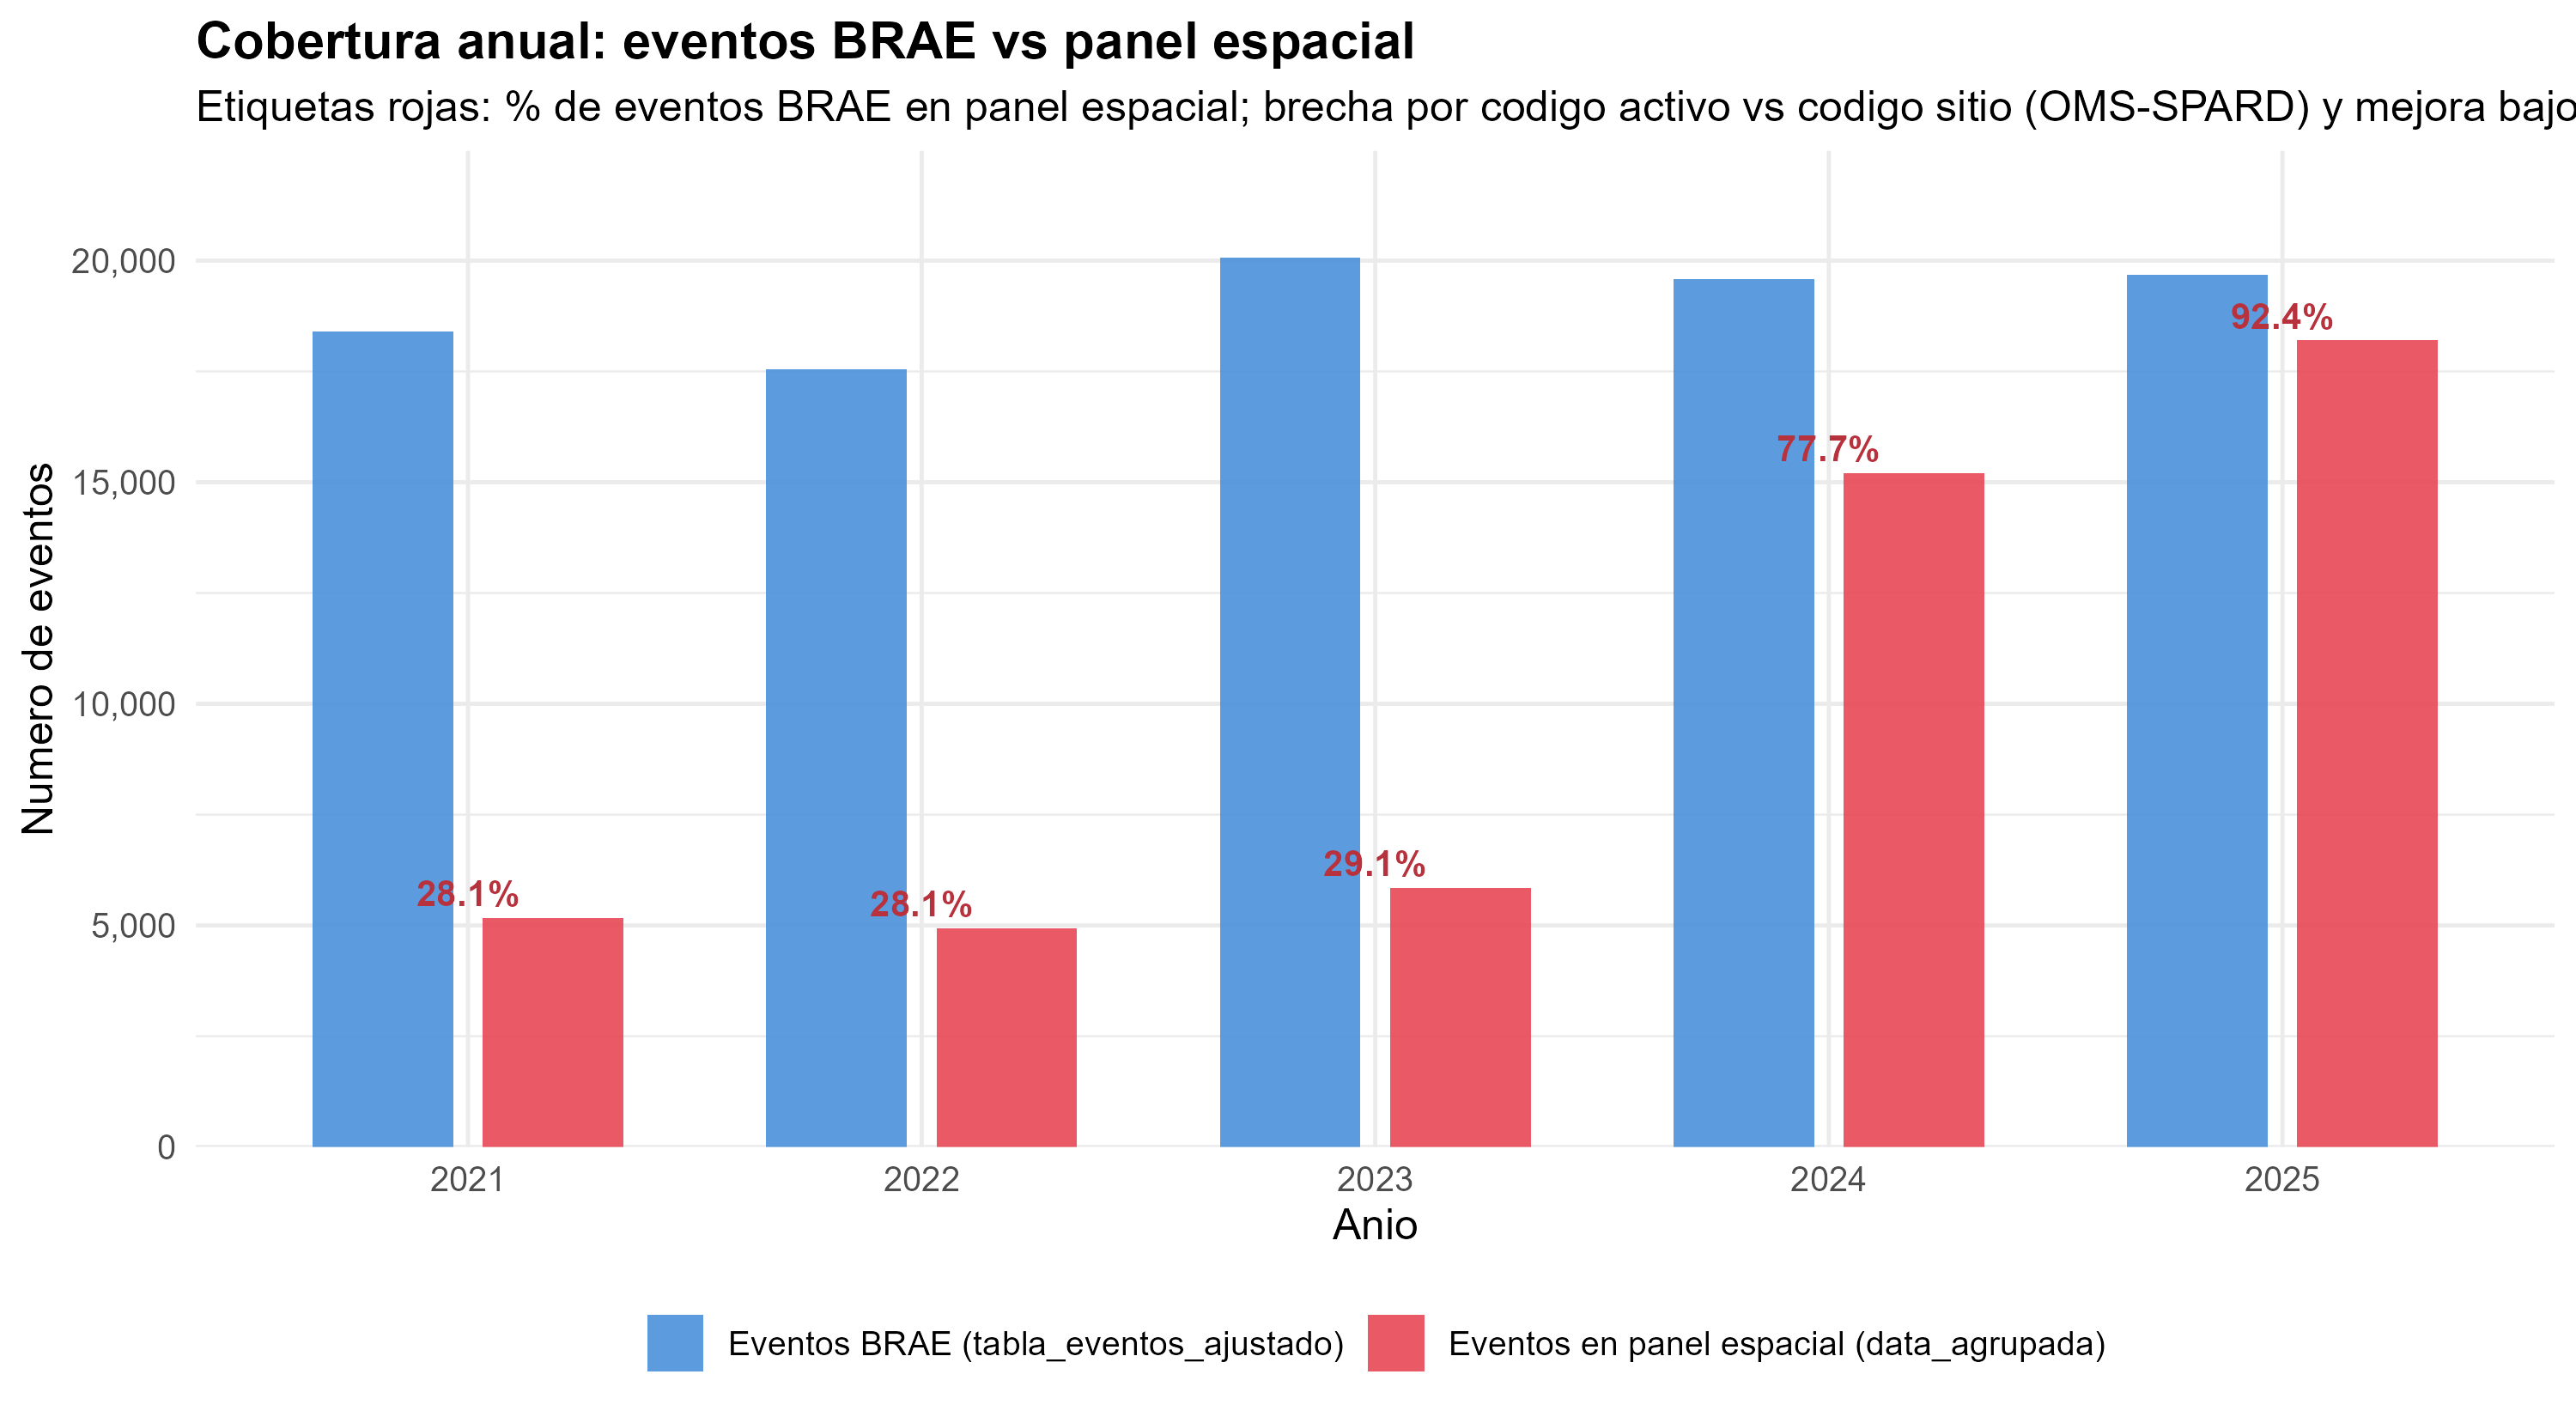
\includegraphics[width=0.95\textwidth]{img/cobertura_emparejamiento_por_anio.png}
        \caption{Comparación anual entre eventos BRAE y eventos reflejados en el panel espacial. Las etiquetas indican el porcentaje de cobertura respecto a BRAE; la brecha histórica se explica por la incompatibilidad entre el código de activo registrado en OMS-SPARD y el código de sitio del inventario GIS.}
        \label{fig:cobertura_emparejamiento}
    \end{figure}
    
    \paragraph{Estacionalidad intra-anual.} La Figura~\ref{fig:estacionalidad_mensual} muestra la distribución de los totales semanales según el mes calendario. Se aprecia heterogeneidad estacional, con mayor actividad y dispersión en algunos meses del año, patrón que motiva incorporar términos estacionales en la Etapa~4. La atribución de esta estacionalidad a la temporada de lluvias debe tomarse con cautela: como se documenta en la Sección~\ref{sec:analisis_correlacion_asociacion}, la asociación semanal entre precipitación y frecuencia de eventos es débil en el grano cuadrante~$\times$~semana.
    
    \begin{figure}[!htbp]
        \centering
        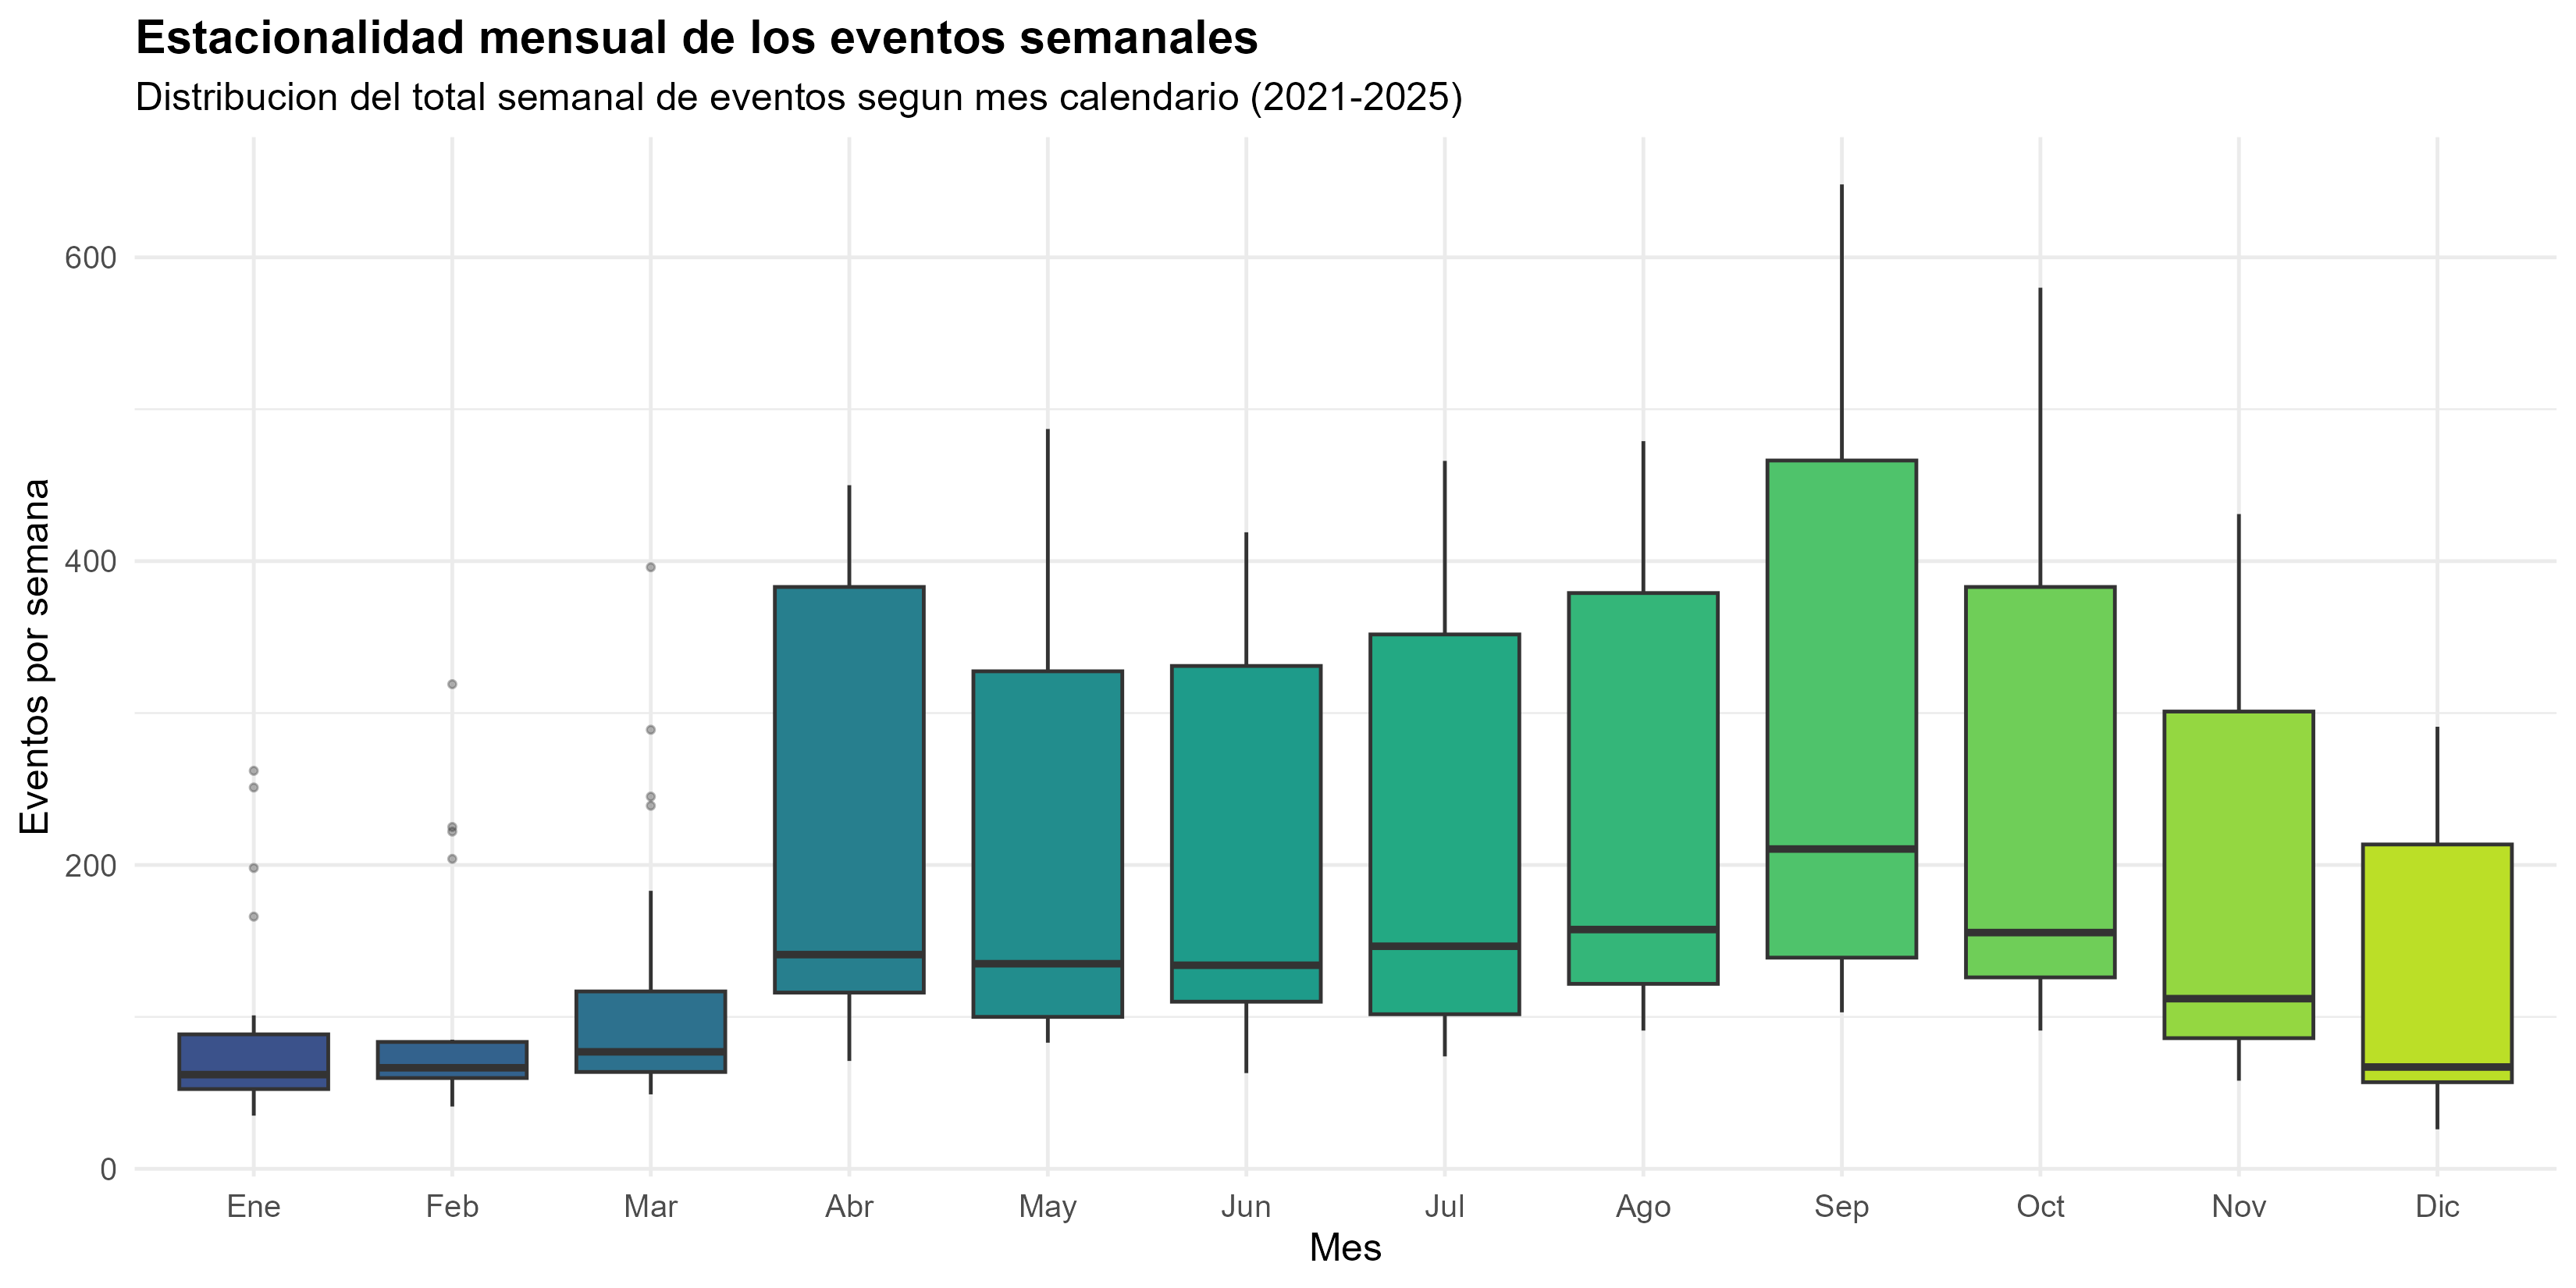
\includegraphics[width=0.95\textwidth]{img/estacionalidad_mensual_eventos_agrupada.png}
        \caption{Distribución del total semanal de eventos según mes calendario (2021--2025).}
        \label{fig:estacionalidad_mensual}
    \end{figure}
    
    \paragraph{Autocorrelación temporal.} Las funciones de autocorrelación simple y parcial de la serie semanal (Figura~\ref{fig:acf_serie_semanal}) evidencian fuerte persistencia: la autocorrelación es $0{.}92$ en el rezago de una semana y decae lentamente ($0{.}60$ a $12$ semanas; $0{.}38$ a $26$), manteniéndose significativa frente al intervalo de confianza del $95$~\% bajo ruido blanco ($\pm 0{.}12$). Adicionalmente, el rezago de $52$ semanas conserva una autocorrelación de $0{.}43$, indicativa de un componente estacional anual. Esta estructura justifica la incorporación de rezagos y términos estacionales como variables predictoras en la Etapa~4.
    
    \begin{figure}[!htbp]
        \centering
        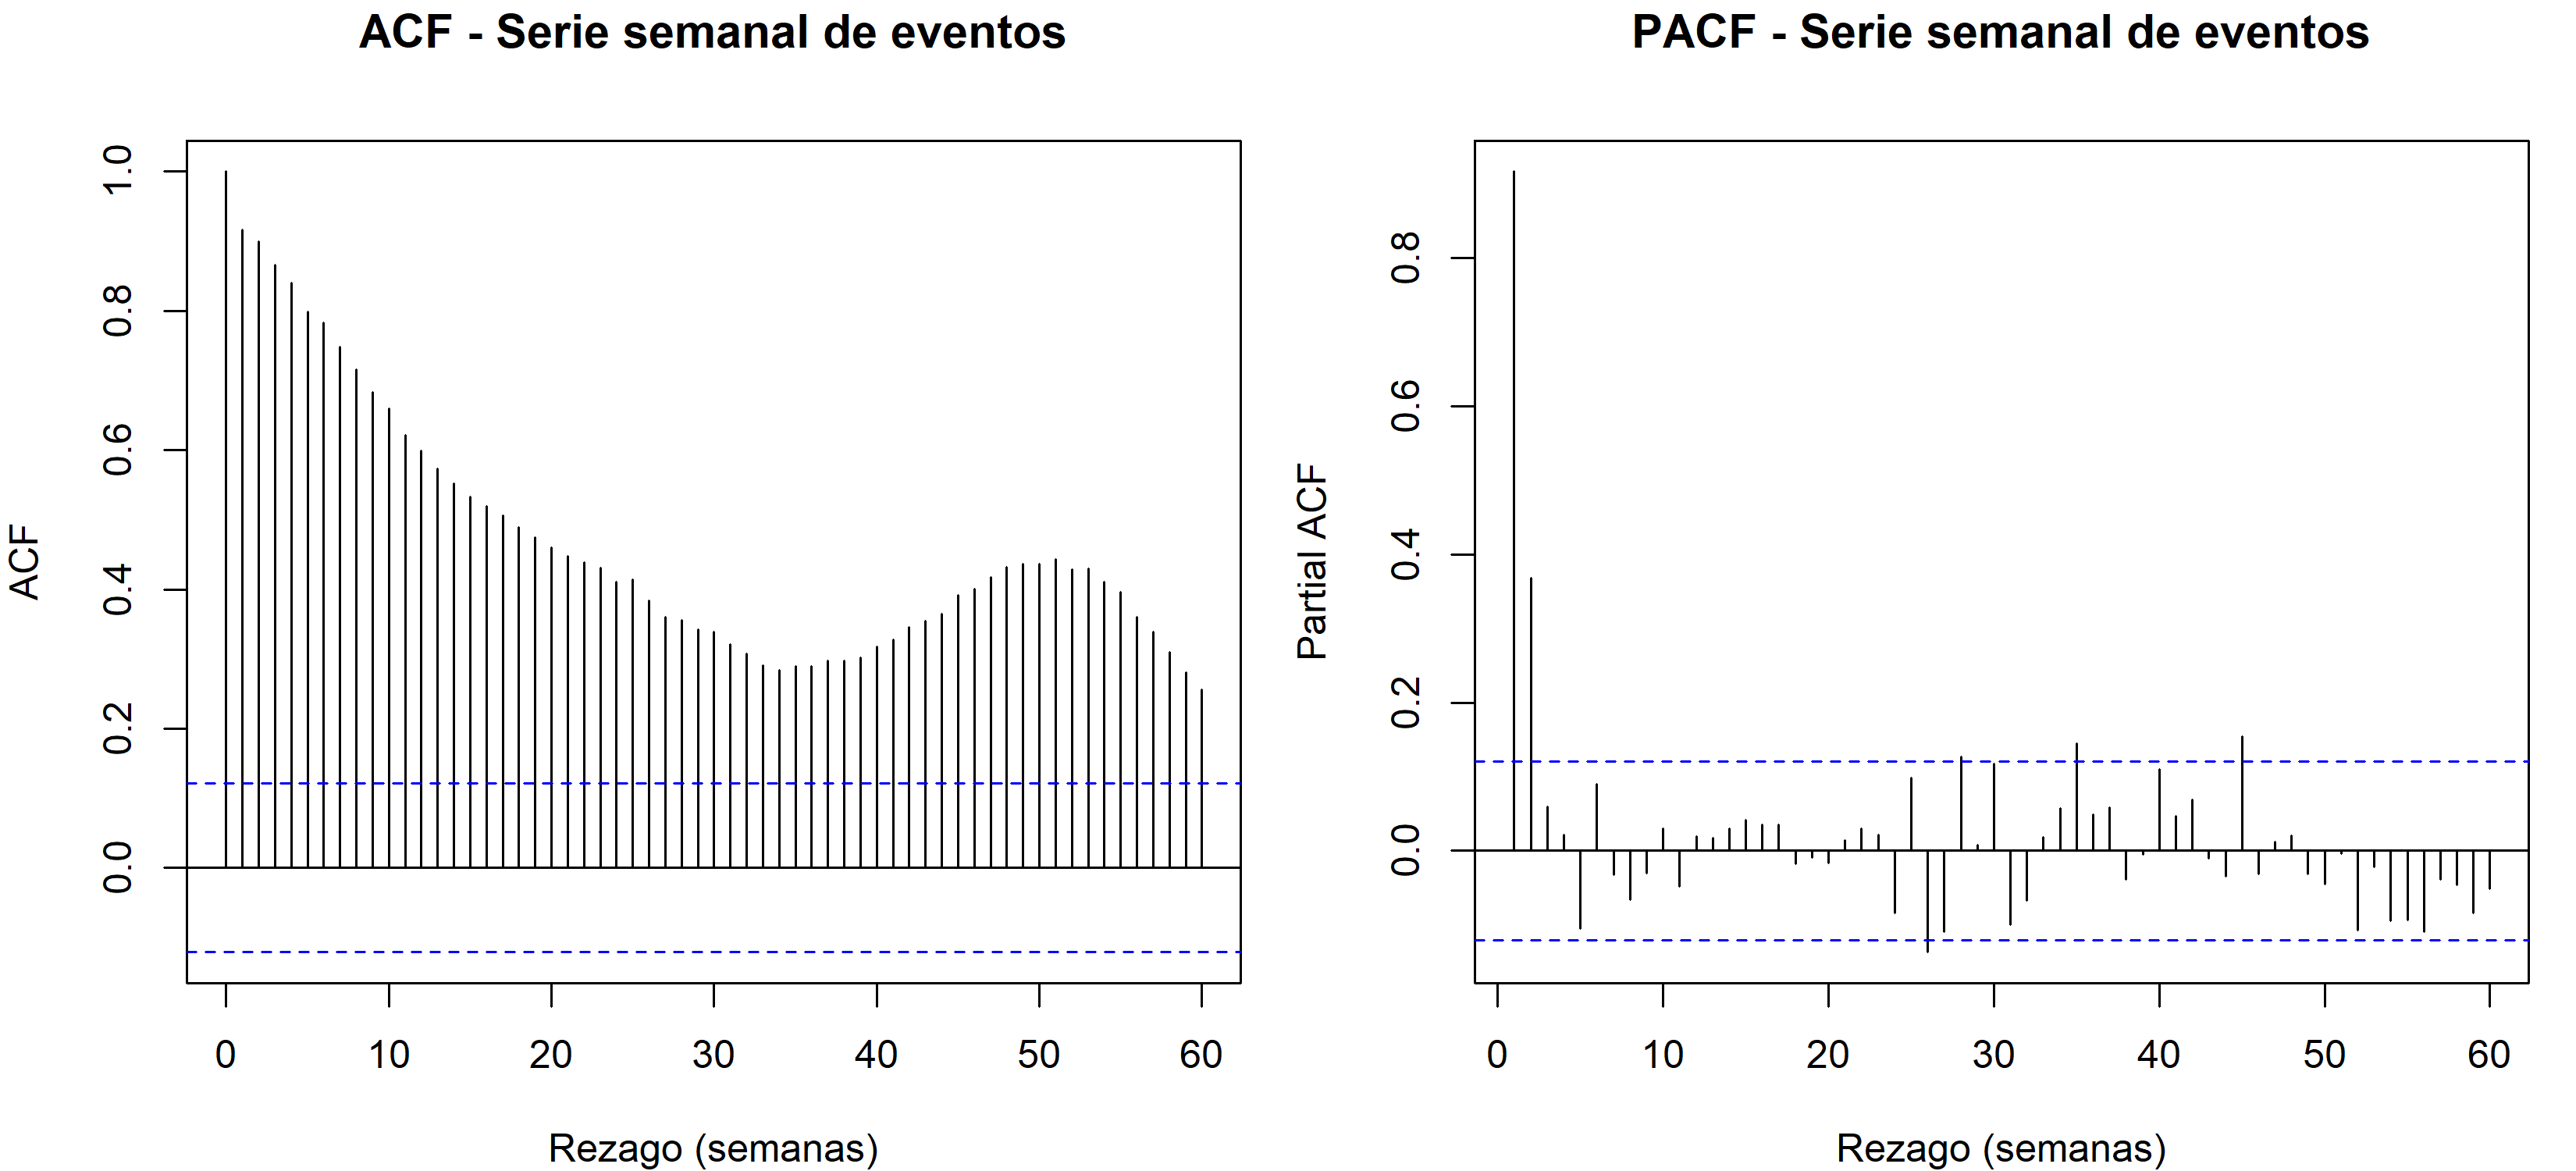
\includegraphics[width=0.95\textwidth]{img/acf_serie_semanal_agrupada.png}
        \caption{Persistencia y estructura temporal de la serie semanal de eventos (rezagos en semanas).}
        \label{fig:acf_serie_semanal}
    \end{figure}
    
    \paragraph{Evolución de la severidad y extensión territorial.} La Figura~\ref{fig:serie_severidad_semanal} presenta las series semanales de usuarios afectados y duración acumulada: ambas acompañan el incremento de nivel observado en la frecuencia de eventos a partir de 2024, lo que indica que el cambio de régimen no es solo de conteo sino también de impacto sobre la continuidad del servicio. Complementariamente, la Figura~\ref{fig:cuadrantes_activos_semana} muestra el número de cuadrantes con al menos un evento por semana, que crece en paralelo: la mayor actividad reciente se distribuye sobre una porción más amplia del territorio y no se explica por unos pocos cuadrantes puntuales.
    
    \begin{figure}[!htbp]
        \centering
        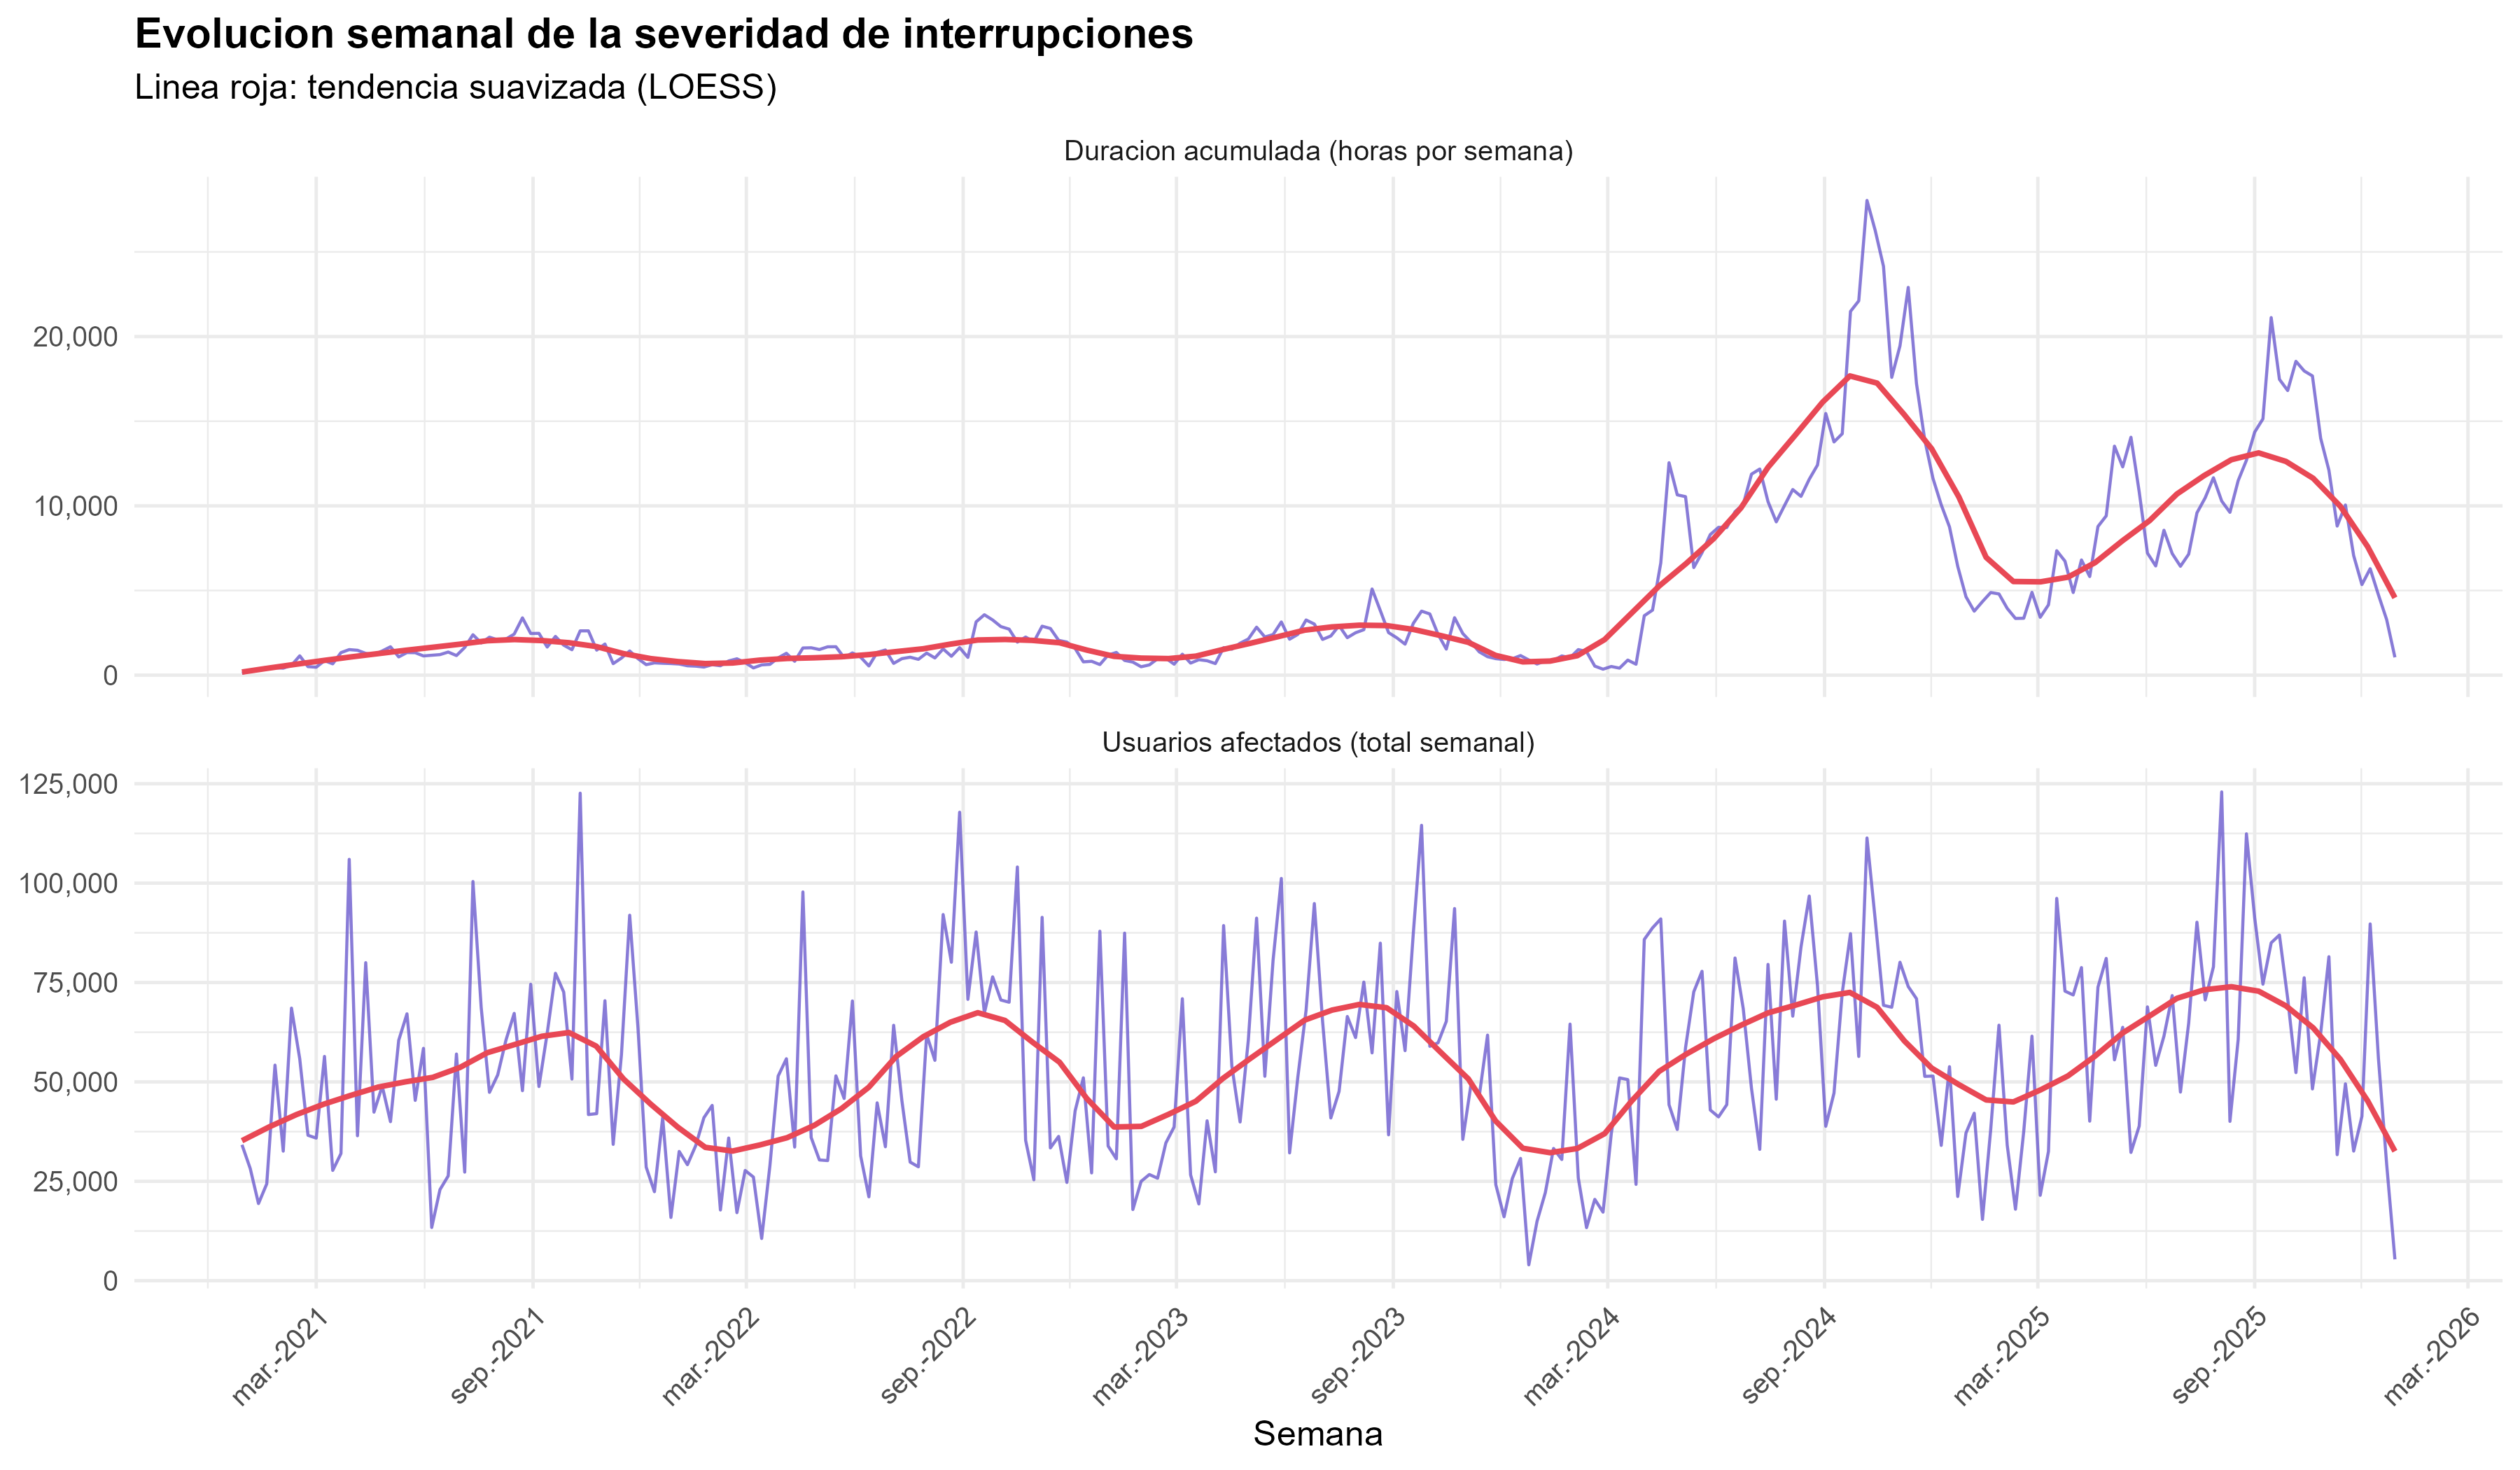
\includegraphics[width=0.95\textwidth]{img/serie_severidad_semanal_agrupada.png}
        \caption{Evolución semanal de usuarios afectados y duración acumulada.}
        \label{fig:serie_severidad_semanal}
    \end{figure}
    
    \begin{figure}[!htbp]
        \centering
        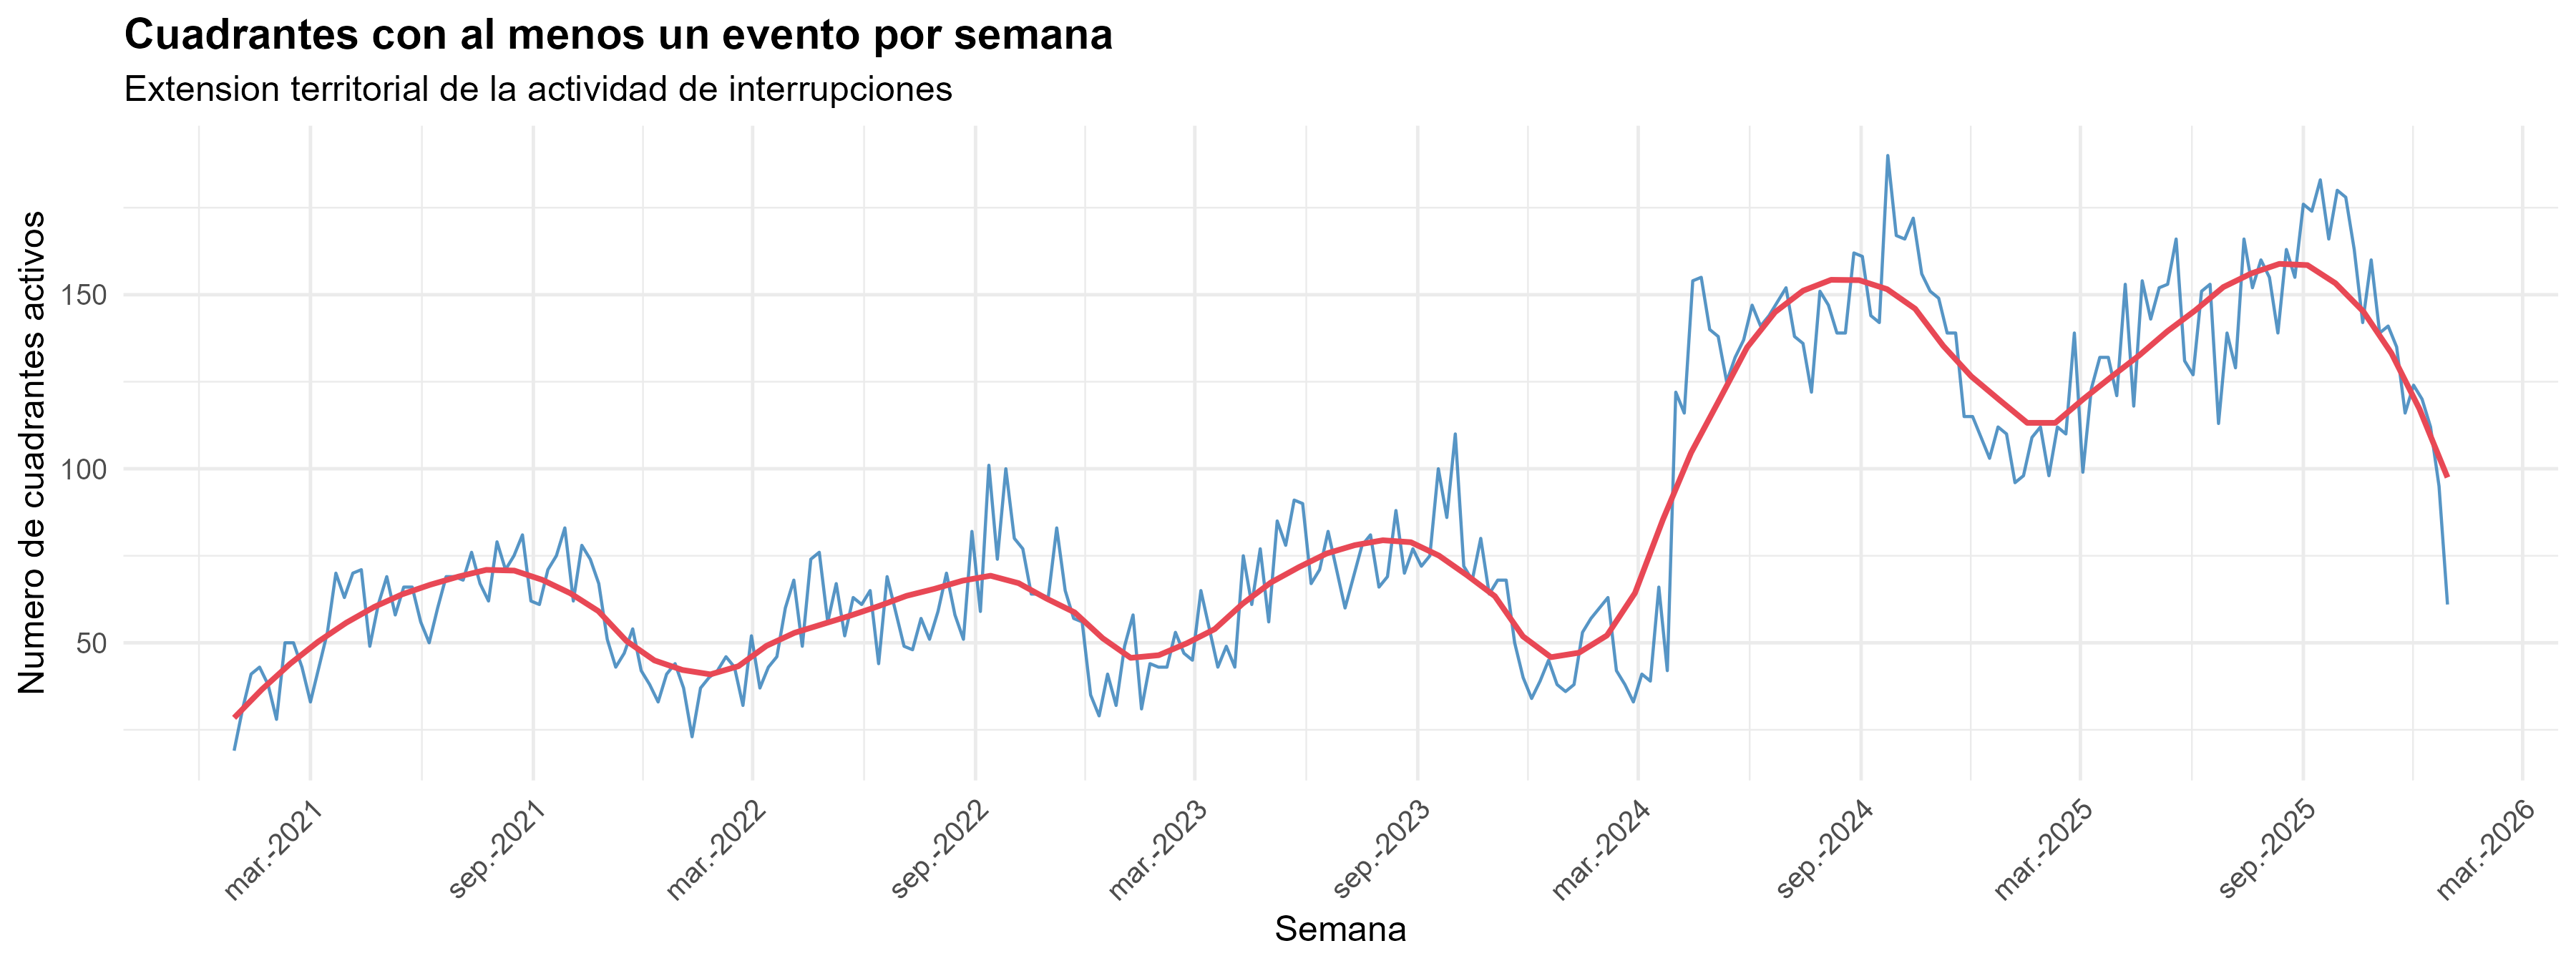
\includegraphics[width=0.95\textwidth]{img/cuadrantes_activos_semana_agrupada.png}
        \caption{Número de cuadrantes con al menos un evento por semana (extensión territorial de la actividad).}
        \label{fig:cuadrantes_activos_semana}
    \end{figure}
    
    \noindent En síntesis, el análisis temporal sobre $D_{\mathrm{EDA}}$ revela: (i)~un cambio de nivel de la serie a partir de 2024, reinterpretado como mayor homogeneización de la codificación activo/sitio bajo OMS-SP7, y no como incremento operativo aislado, lo que motiva la restricción del dataset de modelado a $D_{\mathrm{mod}}$ (2024--2025; Sección~\ref{sec:delimitacion_temporal_modelado}); (ii)~estacionalidad intra-anual en la actividad de interrupciones, cuya atribución al régimen de lluvias no se sostiene con el acumulado semanal de precipitación (Sección~\ref{sec:analisis_correlacion_asociacion}); y (iii)~fuerte persistencia semanal con componente anual, que fundamenta el uso de rezagos temporales como predictores en $D_{\mathrm{mod}}$. Estos hallazgos orientan la generación de ventanas temporales y la partición de datos de la Etapa~4.
    
    \paragraph{Materialización de $D_{\mathrm{mod}}$.} Para operacionalizar la delimitación temporal sin alterar el insumo exploratorio, se construyó el archivo \texttt{data\_agrupada\_mod.csv} como subconjunto de \texttt{data\_agrupada.csv} con filtro \texttt{year(semana)} $\in \{2024,\,2025\}$, conservando el grano cuadrante~$\times$~semana y el conjunto completo de variables climáticas y operativas. La tabla original 2021--2025 permanece intacta como $D_{\mathrm{EDA}}$; el resultado filtrado ($36\,120$ filas; $344$ cuadrantes; $105$ semanas; $33\,410$ eventos) constituye el insumo analítico para las Secciones~\ref{sec:identificacion_patrones_tendencias} en adelante y la Etapa~4, con partición natural entrenamiento 2024 / prueba 2025. El procedimiento reproducible, lectura, filtro, resumen por año y exportación, se documenta en el Apéndice~\ref{app:html-datamod}.

    \paragraph{Enriquecimiento de $D_{\mathrm{mod}}$.} Sobre la llave
    cuadrante--semana se incorporaron 16 variables destinadas a ampliar la
    caracterización de exposición, composición de usuarios y trayectoria de
    intervención de los activos. La serie mensual
    \texttt{data\_usuarios\_totales\_sistema.csv} aporta
    \texttt{usuarios\_totales}, asignada a cada semana de acuerdo con el mes
    calendario de su fecha de inicio y utilizada como denominador en la
    construcción de SAIDI y SAIFI. Por otra parte,
    \texttt{cant\_usuarios\_x\_transformador.csv} aporta
    \texttt{cantidad\_usuarios\_cuadrante}, calculada como la suma mensual de
    usuarios de los transformadores asociados a cada cuadrante.

    La composición socioeconómica y de uso del servicio se integró desde
    \texttt{DATA\_ESTRATO\_SECTOR.csv}, agregando por cuadrante y mes las
    variables \texttt{ESTRATO\_1} a \texttt{ESTRATO\_6},
    \texttt{INDUSTRIAL}, \texttt{COMERCIAL}, \texttt{OFICIAL},
    \texttt{PROVISIONAL} y \texttt{ALUMBRADO\_PUBLICO}. Para los meses
    faltantes de los cuadrantes 258 y 273 se empleó la moda mensual del
    respectivo cuadrante; los cuadrantes 68, 140, 333 y 344, ausentes en la
    fuente, se asignaron en cero.

    Finalmente, mediante la llave \texttt{ID\_CUADRANTE} se integró
    \texttt{Fecha\_transformadores.csv}. Para cada elemento se contabilizaron
    sus registros de modificación y se tomó la última
    \texttt{TT2\_FMODIFICACION} en estado \texttt{OPERACION}; posteriormente,
    por cuadrante, se derivaron \texttt{FECHA\_ACTIVO\_MAS\_VIEJO},
    \texttt{FECHA\_ACTIVO\_MAS\_NUEVO} y
    \texttt{PROM\_CANT\_MODIFICACIONES}. Estas variables permiten evaluar la
    relación entre la trayectoria de intervención de la infraestructura y los
    indicadores de continuidad. No obstante, las fechas representan
    modificaciones registradas y no necesariamente la instalación original
    del activo. Para evitar fuga de información, su uso predictivo debe
    restringirse a registros conocidos antes de la semana pronosticada;
    SAIDI y SAIFI se emplean exclusivamente como variables objetivo.

\subsection{Identificación de patrones, tendencias y visualización exploratoria}
\label{sec:identificacion_patrones_tendencias}
    Con fundamento en la delimitación de $D_{\mathrm{mod}}$ (Sección~\ref{sec:delimitacion_temporal_modelado}), se identifican patrones temporales, espaciales y de asociación clima--evento sobre la tabla \texttt{data\_agrupada\_mod.csv} ($36\,120$ filas cuadrante~$\times$~semana; $344$ cuadrantes; $105$ semanas; $33\,410$ eventos en 2024--2025). En esta misma subsección se integra la \textit{visualización exploratoria} sobre $D_{\mathrm{mod}}$: series de tiempo, diagramas de dispersión y mapas temáticos que complementan el análisis cuantitativo de patrones. El procedimiento reproducible se documenta en el Apéndice~\ref{app:html-patrones}.
    
    \paragraph{Patrones temporales.} La Figura~\ref{fig:serie_semanal_patrones_mod} presenta la serie semanal territorial de eventos en $D_{\mathrm{mod}}$, con media de $\approx 318$ eventos por semana. Aunque las etiquetas del eje horizontal se muestran cada 3 meses para facilitar la lectura, cada tramo de la linea corresponde a observaciones semanales consecutivas. La intensidad promedio asciende de $287$ eventos/semana en 2024 a $350$ en 2025. La estacionalidad mensual (Figura~\ref{fig:estacionalidad_patrones_mod}) confirma la heterogeneidad entre meses observada en la Sección~\ref{sec:analisis_temporal_eventos} sobre $D_{\mathrm{EDA}}$, sin que el acumulado semanal de lluvia explique ese patrón. La ACF de la serie semanal (Figura~\ref{fig:acf_patrones_mod}) mantiene persistencia elevada (rezago~$1 = 0{.}80$), lo que respalda el uso de rezagos como predictores en la Etapa~4.
    
    \begin{figure}[!htbp]
        \centering
        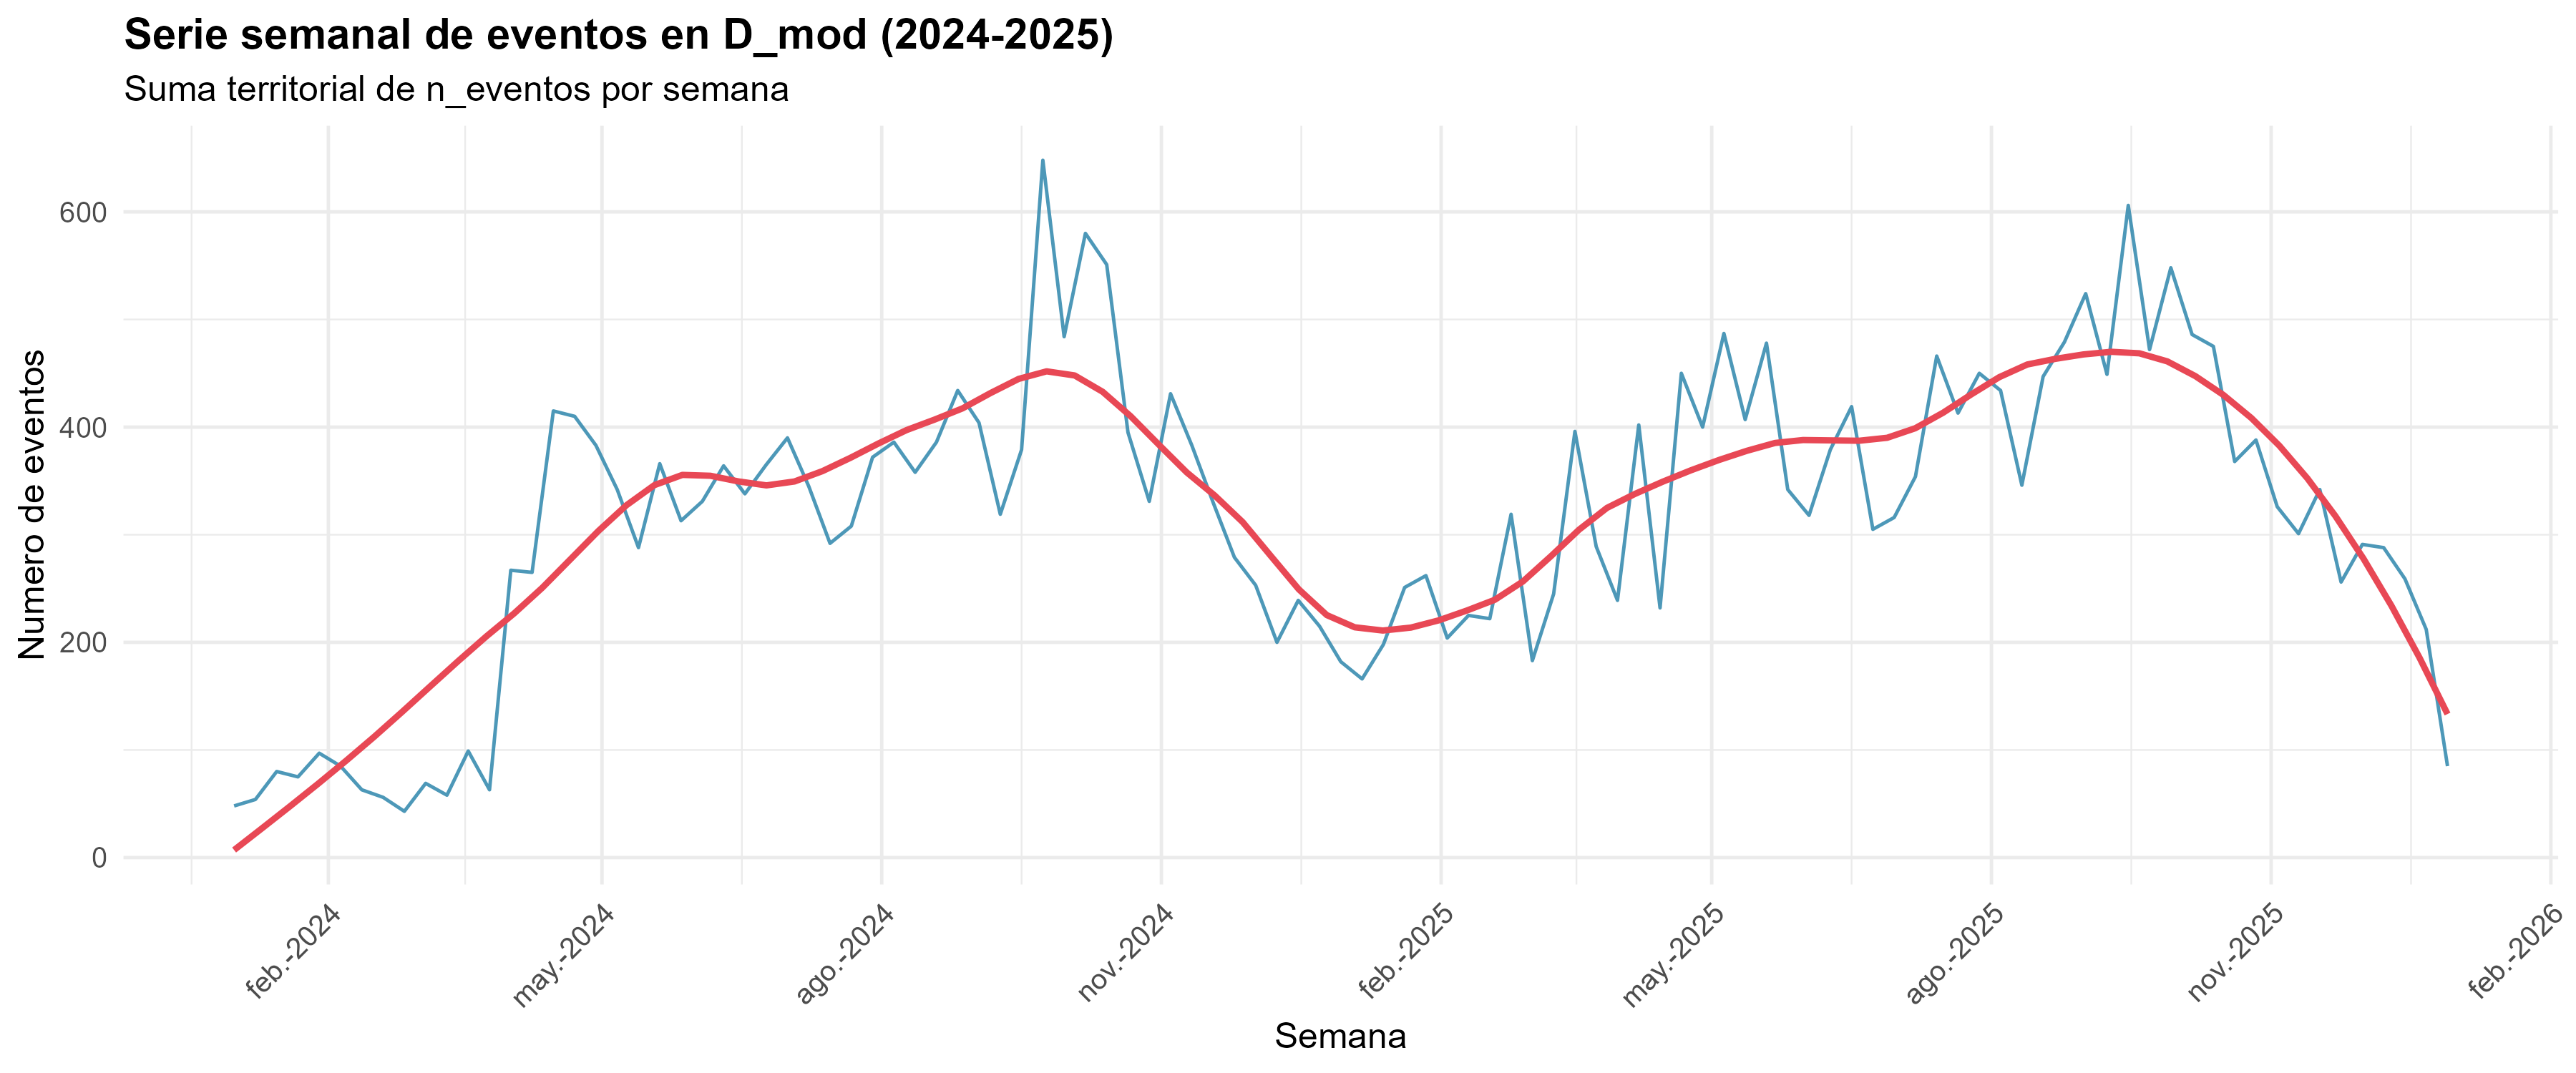
\includegraphics[width=0.95\textwidth]{img/serie_semanal_patrones_mod.png}
        \caption{Evolución semanal de eventos sobre $D_{\mathrm{mod}}$ (2024--2025).}
        \label{fig:serie_semanal_patrones_mod}
    \end{figure}
    
    \begin{figure}[!htbp]
        \centering
        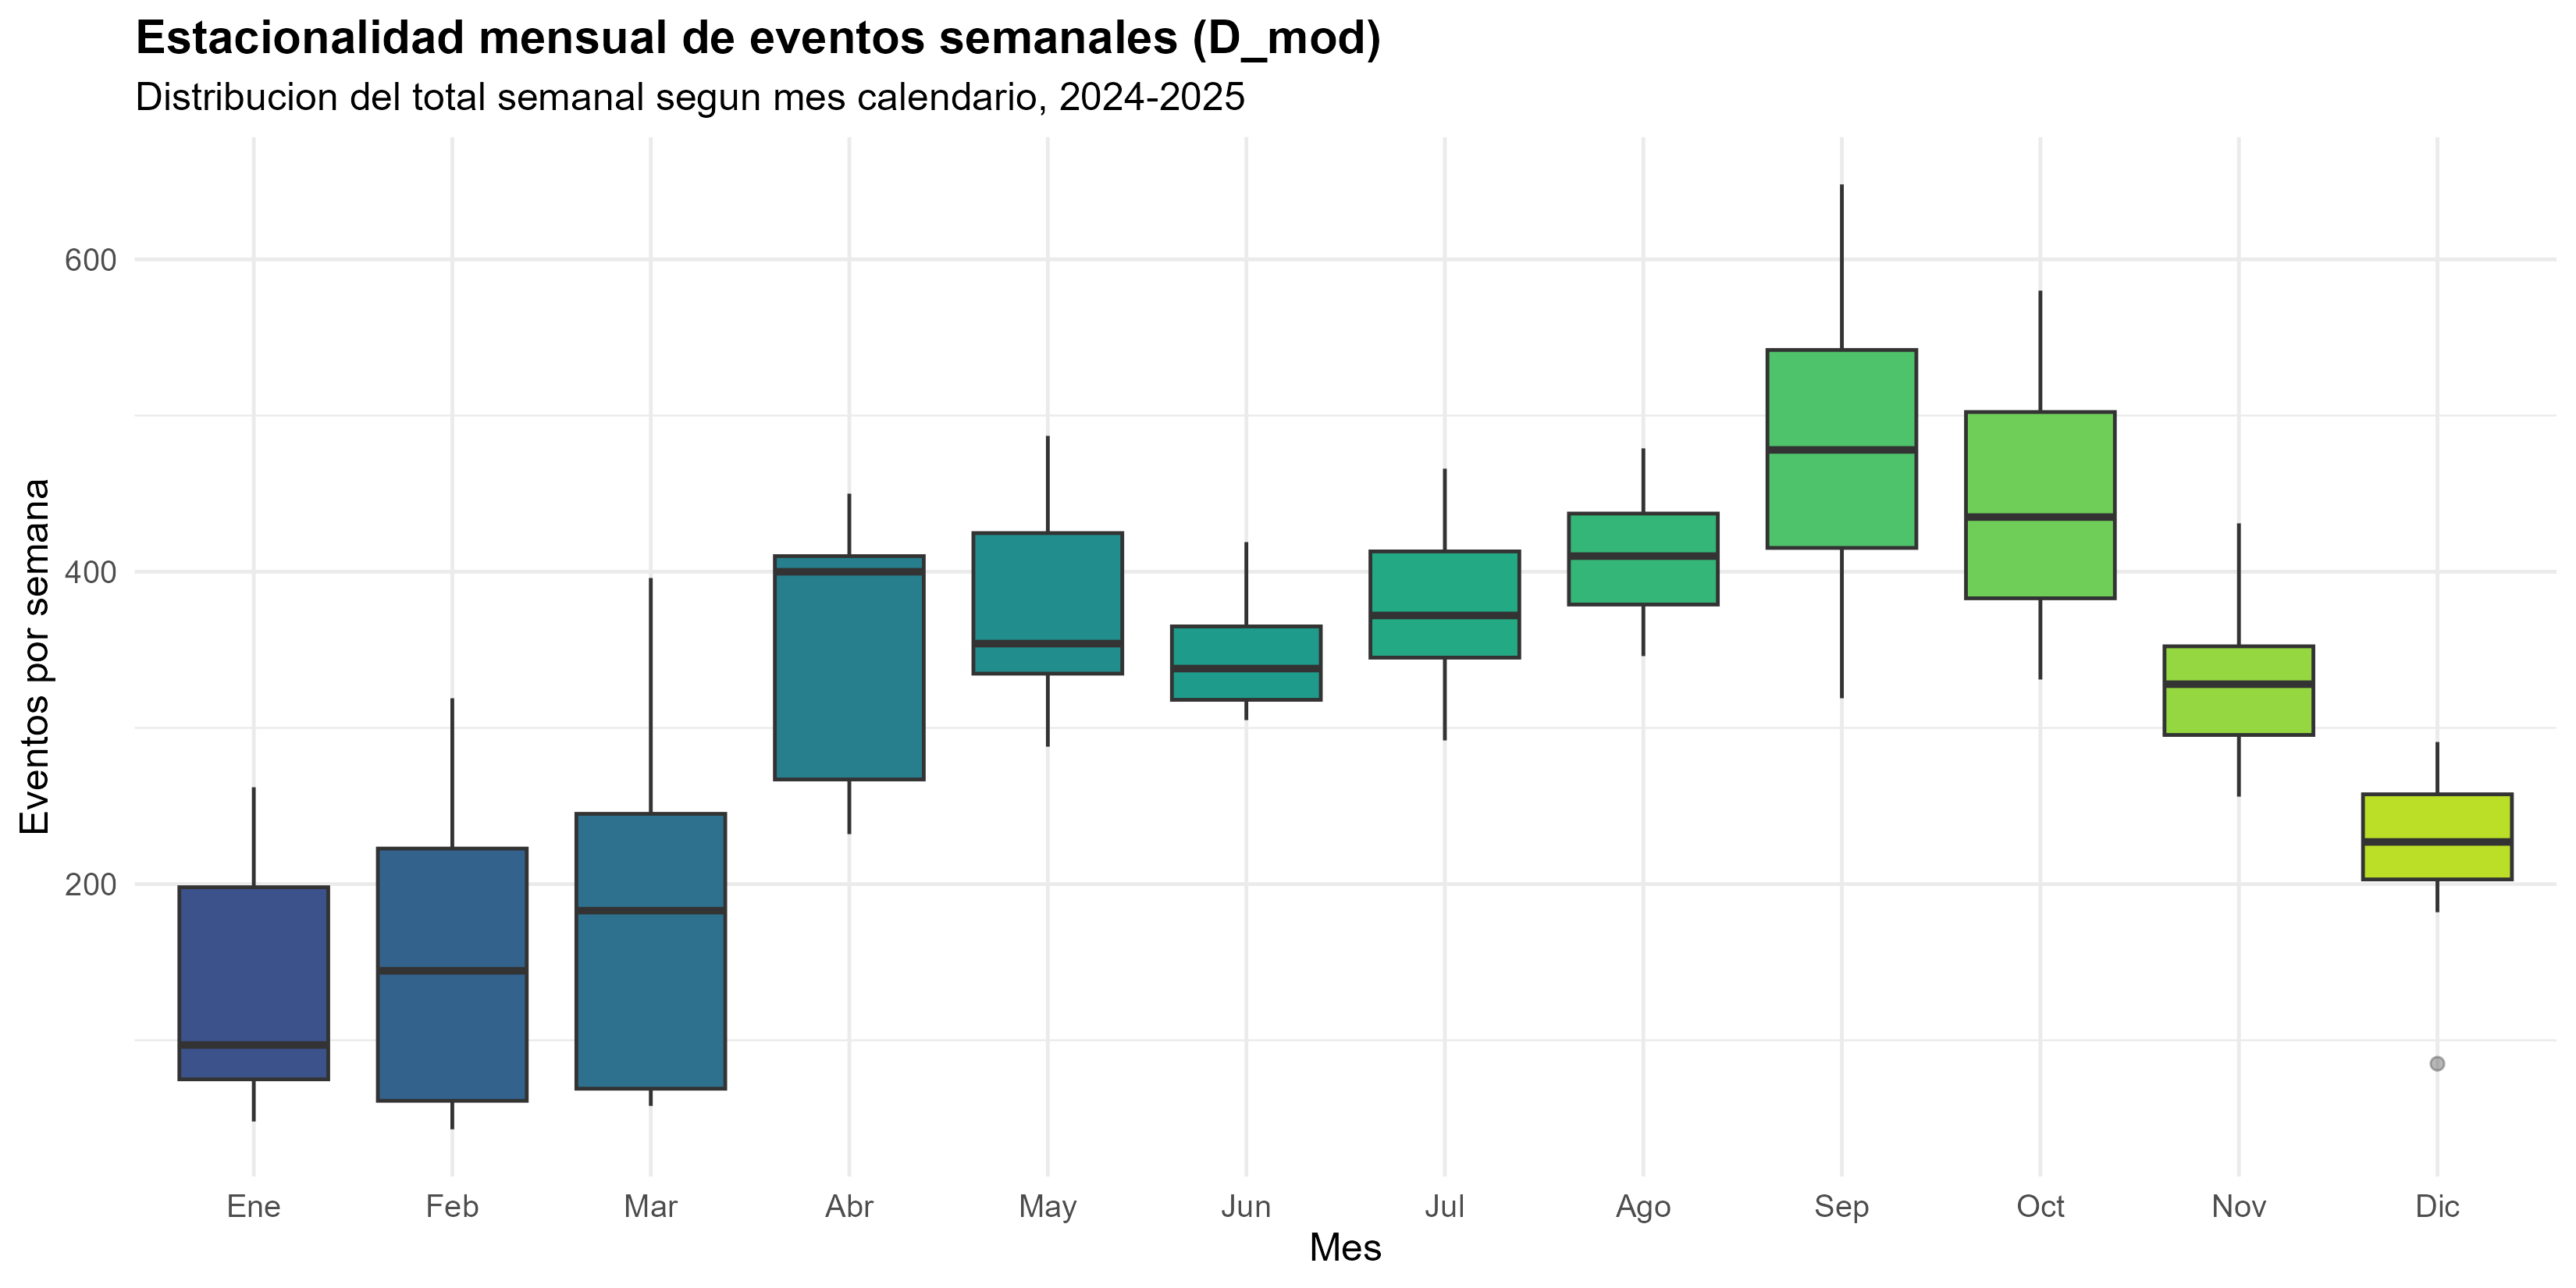
\includegraphics[width=0.95\textwidth]{img/estacionalidad_mensual_patrones_mod.png}
        \caption{Estacionalidad mensual del total semanal de eventos en $D_{\mathrm{mod}}$.}
        \label{fig:estacionalidad_patrones_mod}
    \end{figure}
    
    \begin{figure}[!htbp]
        \centering
        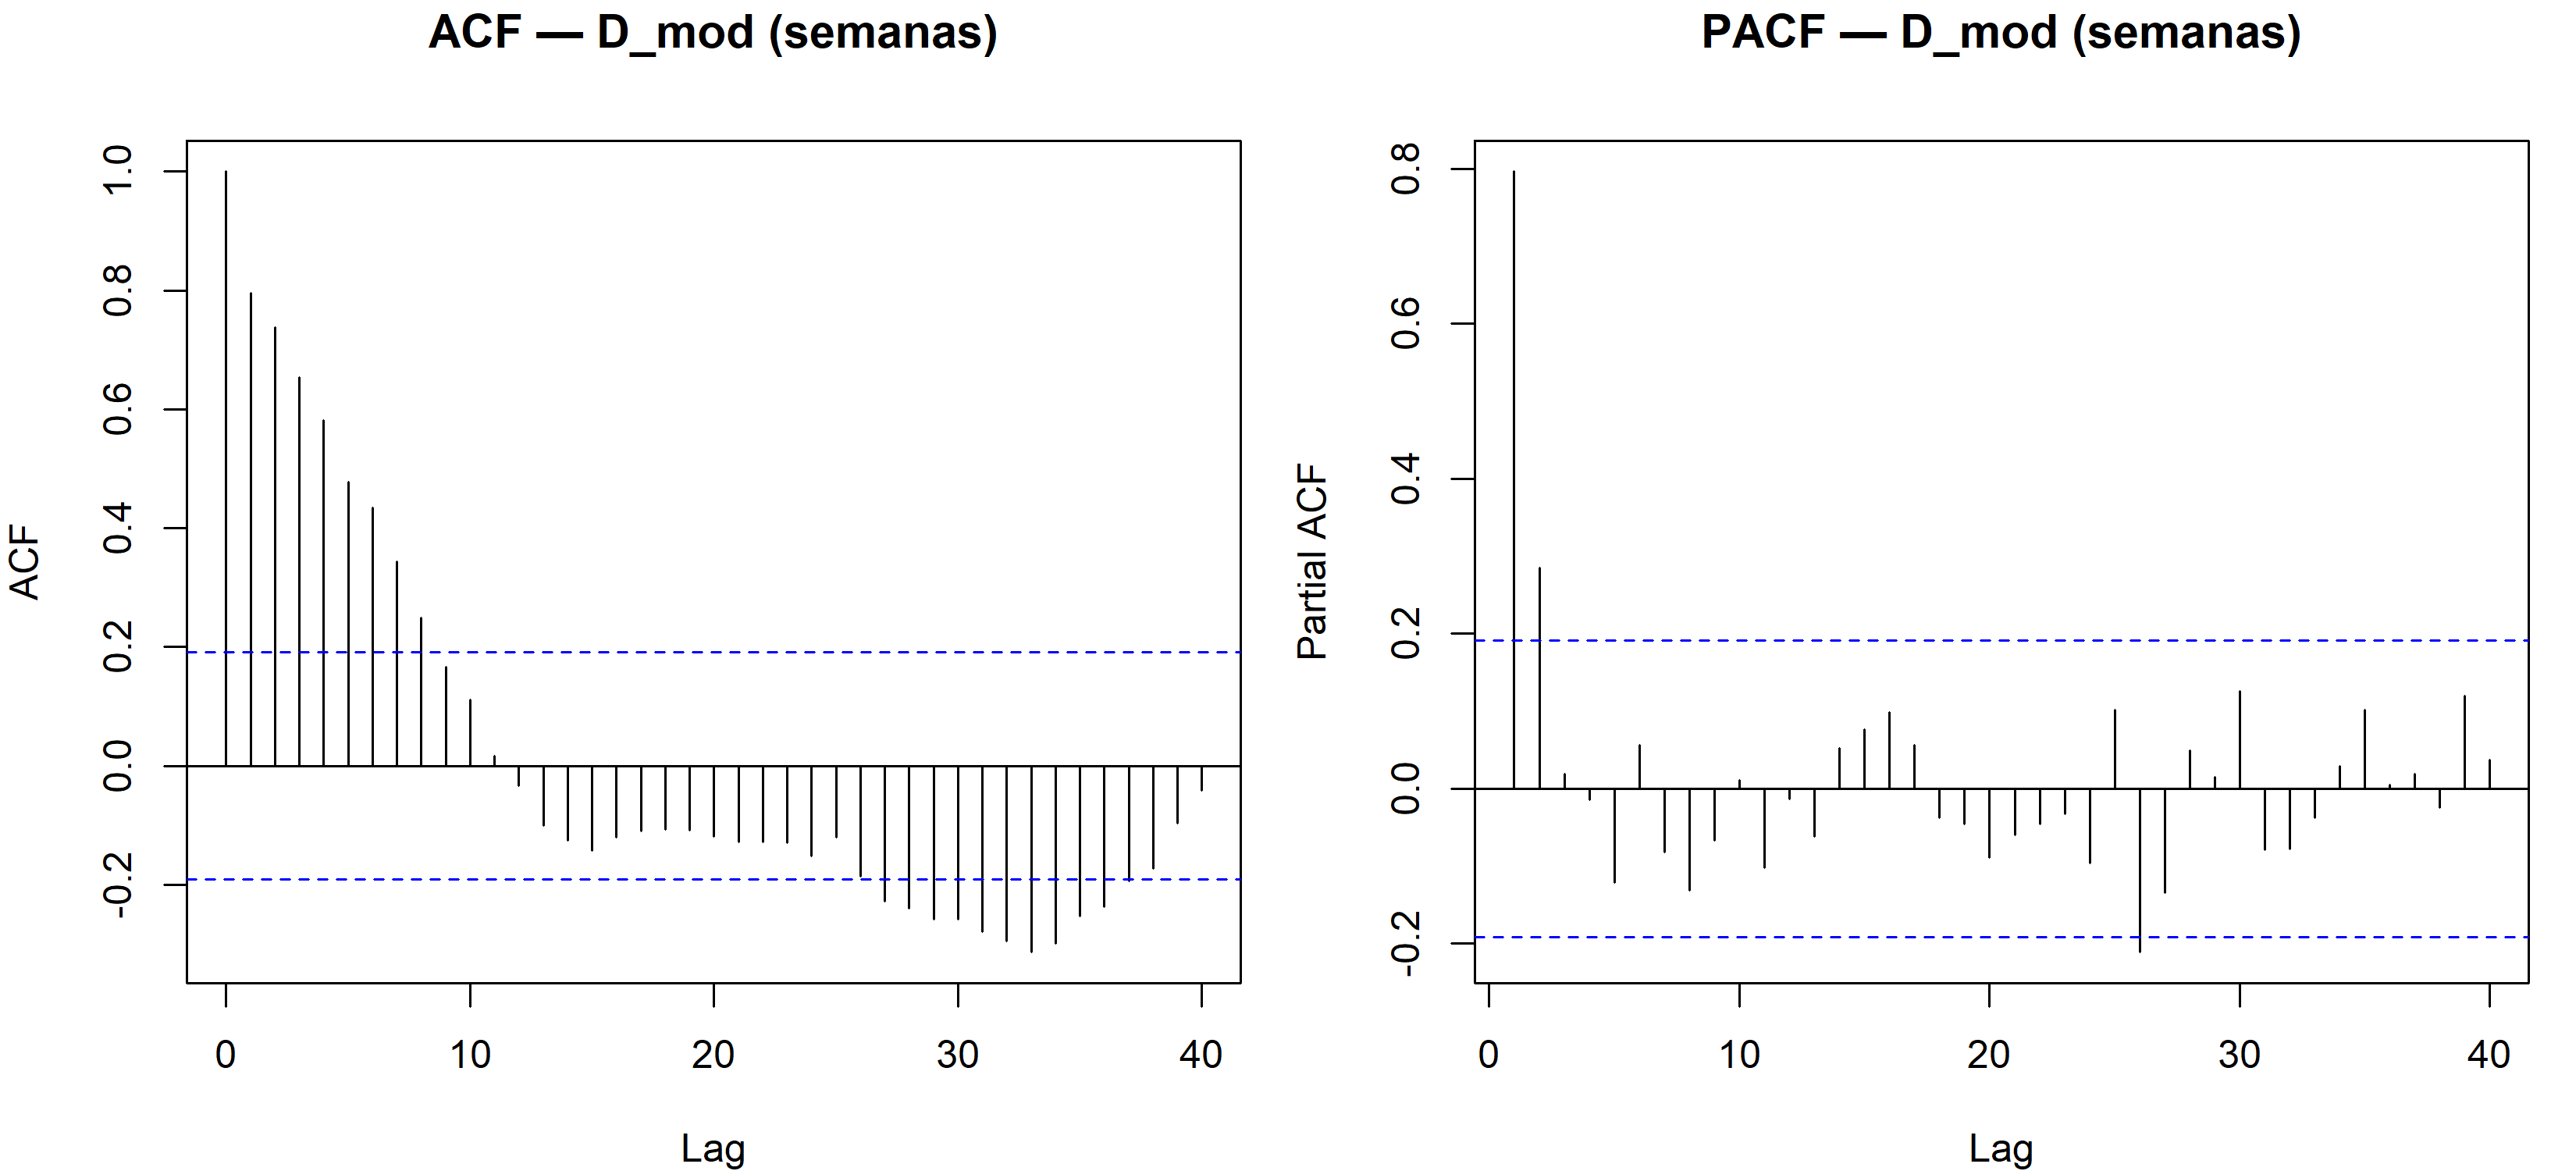
\includegraphics[width=0.95\textwidth]{img/acf_serie_patrones_mod.png}
        \caption{Persistencia y estructura temporal de la serie semanal de eventos en $D_{\mathrm{mod}}$.}
        \label{fig:acf_patrones_mod}
    \end{figure}
    
    \paragraph{Patrones espaciales.} El ranking de cuadrantes por total de \texttt{n\_eventos} (Figura~\ref{fig:ranking_cuadrantes_mod}) y el mapa de intensidad territorial (Figura~\ref{fig:mapa_intensidad_mod}) evidencian heterogeneidad espacial: los diez cuadrantes más activos concentran el $20{.}5$~\% de los eventos del periodo, mientras el $14{.}2$~\% de los cuadrantes ($49$ de $344$) se clasifica en nivel de actividad \emph{alta} (Figura~\ref{fig:segmentacion_mod}). La actividad no se distribuye de forma uniforme sobre la malla de $800$ cuadrantes, sino que se agrupa en zonas de mayor exposición operativa.
    
    \begin{figure}[!htbp]
        \centering
        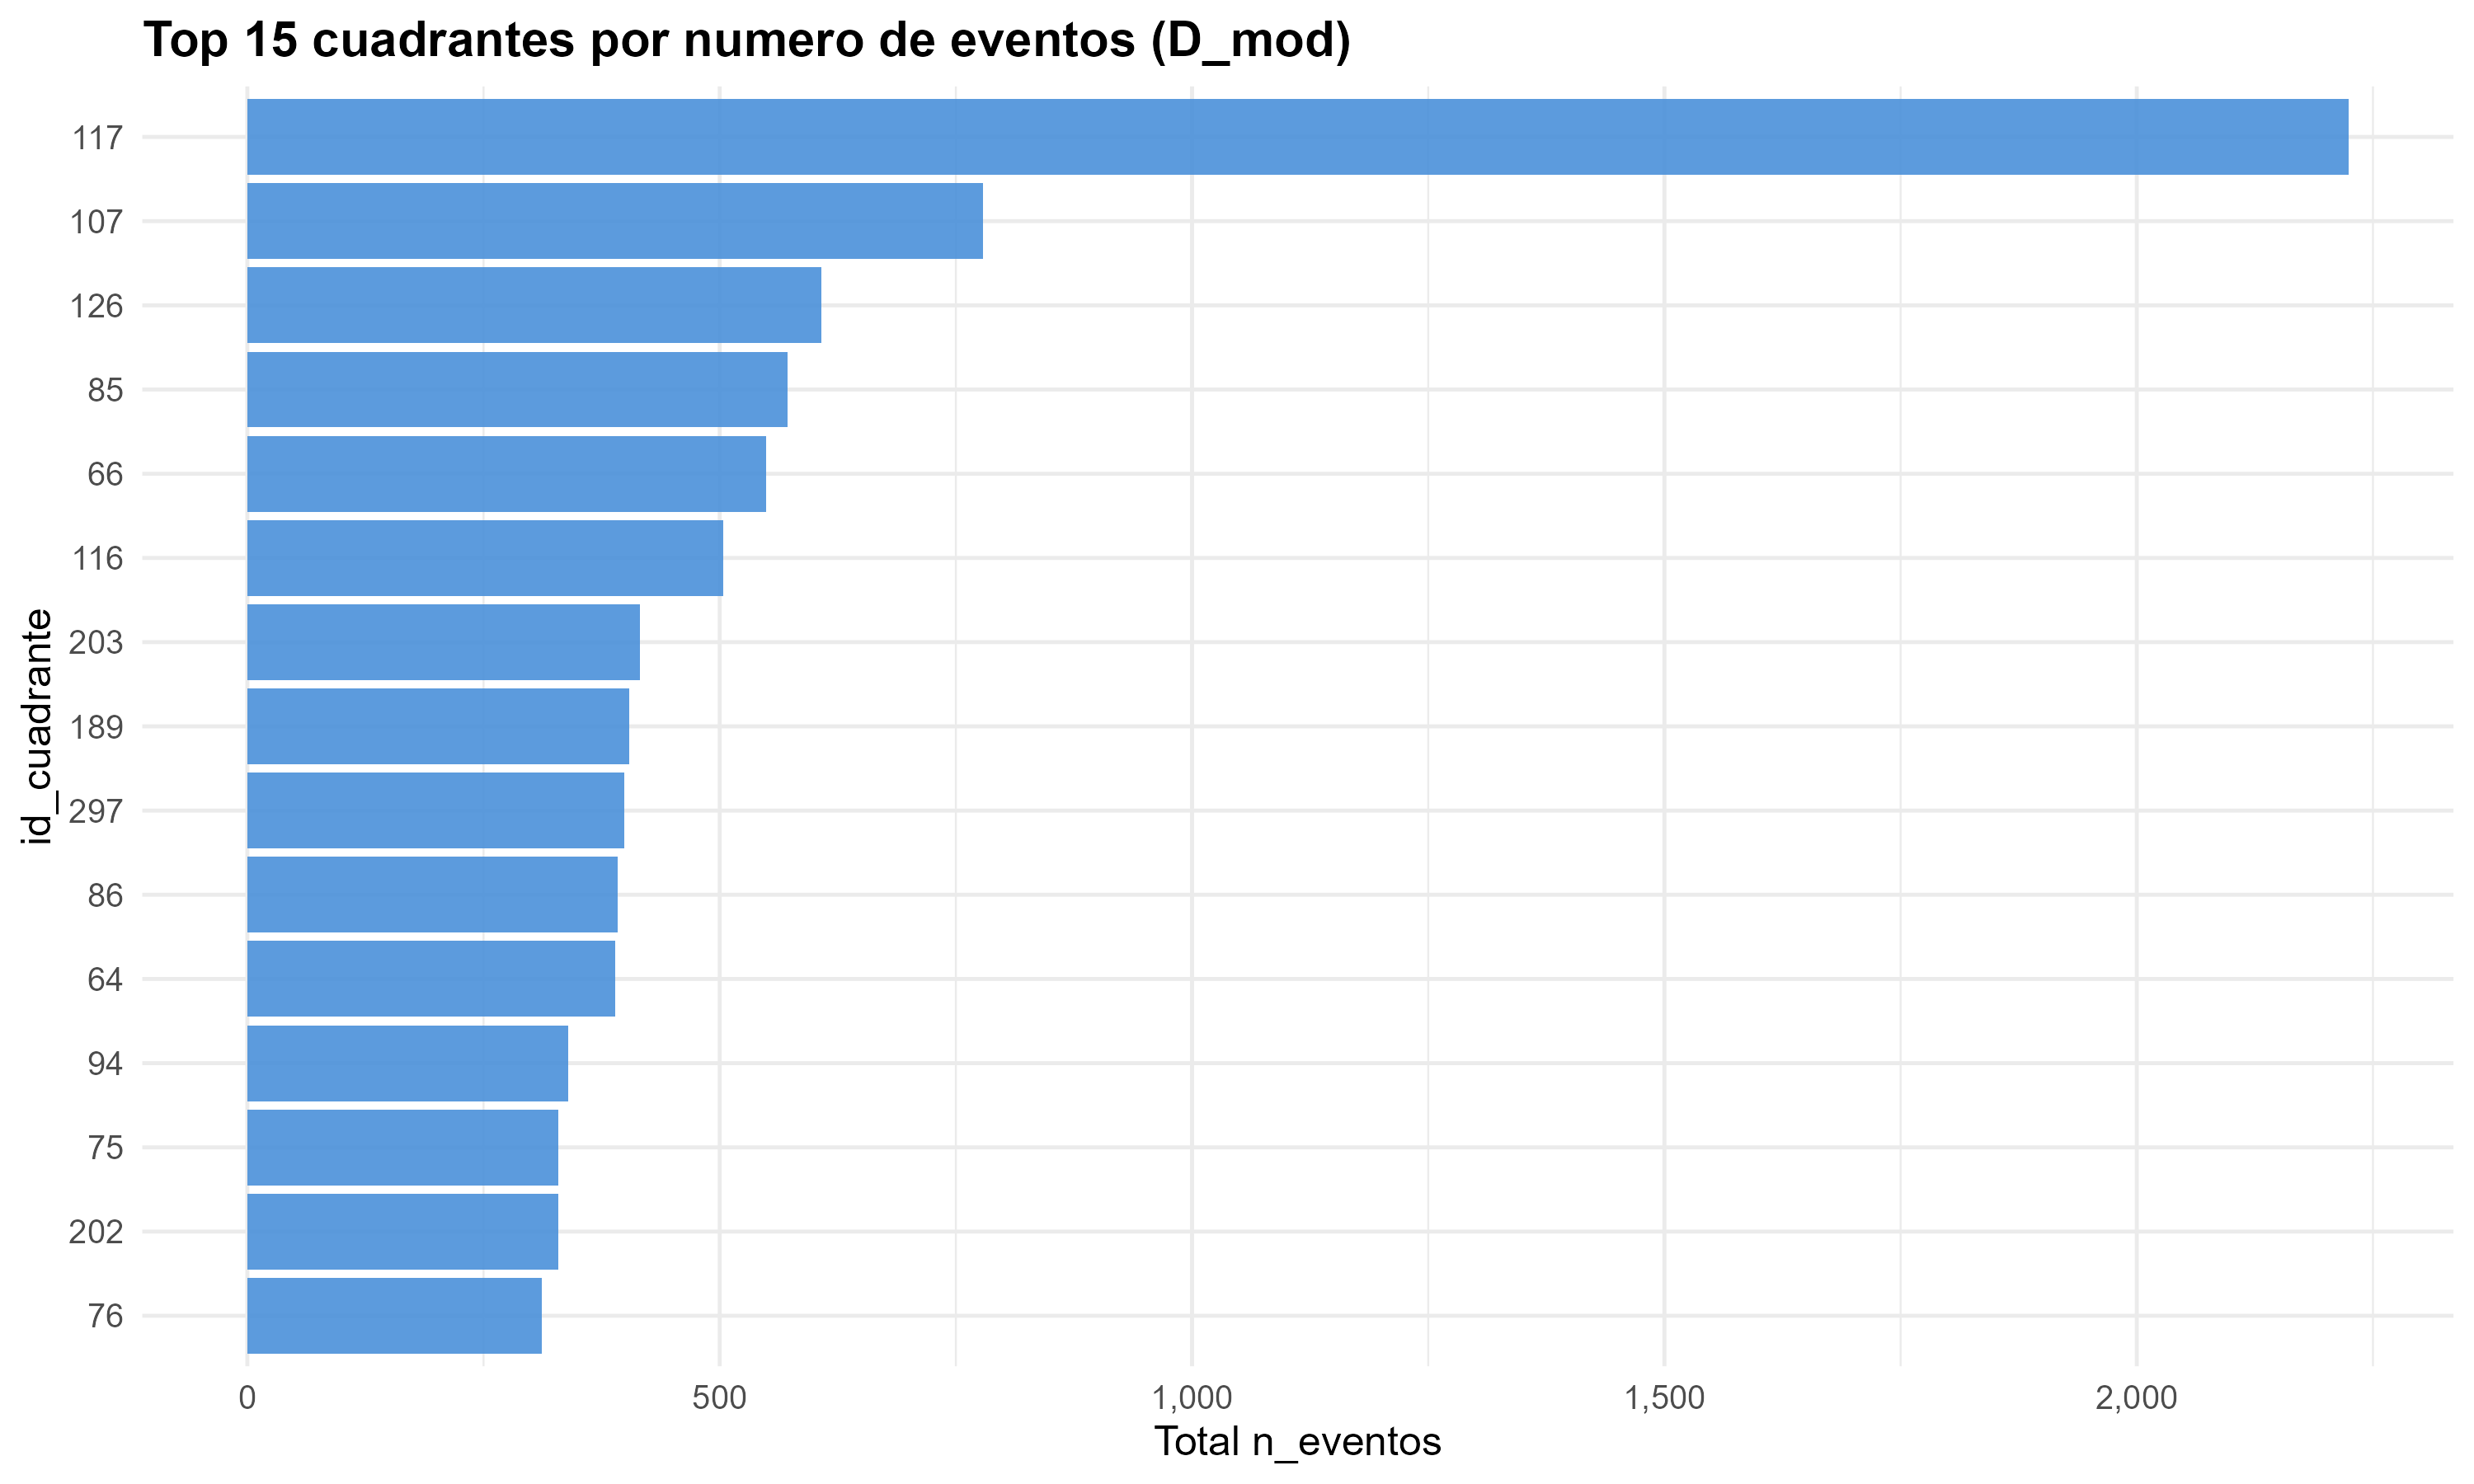
\includegraphics[width=0.85\textwidth]{img/ranking_cuadrantes_patrones_mod.png}
        \caption{Quince cuadrantes con mayor número acumulado de eventos en $D_{\mathrm{mod}}$.}
        \label{fig:ranking_cuadrantes_mod}
    \end{figure}
    
    \noindent La Figura~\ref{fig:ubicacion_top_cuadrantes_mod} complementa el ranking anterior con la \textit{ubicación geográfica} de los cuadrantes más activos sobre la malla territorial del área de estudio. Los recuadros resaltados corresponden a los primeros cuadrantes \emph{top} del periodo 2024--2025 y muestran una concentración en cuatro zonas: (i)~el área metropolitana de Cúcuta y Villa del Rosario; (ii)~un corredor al suroccidente, en torno a Salazar, Arboledas, Durania y Chinácota; (iii)~la subregión de Tibú, al norte del departamento; y (iv)~los municipios de Ocaña y Aguachica, al occidente. Esta distribución espacial confirma que la mayor actividad de interrupciones no es aleatoria, sino que se agrupa en núcleos urbanos y corredores de servicio de la red.
    
    
    \begin{figure}[!htbp]
        \centering
        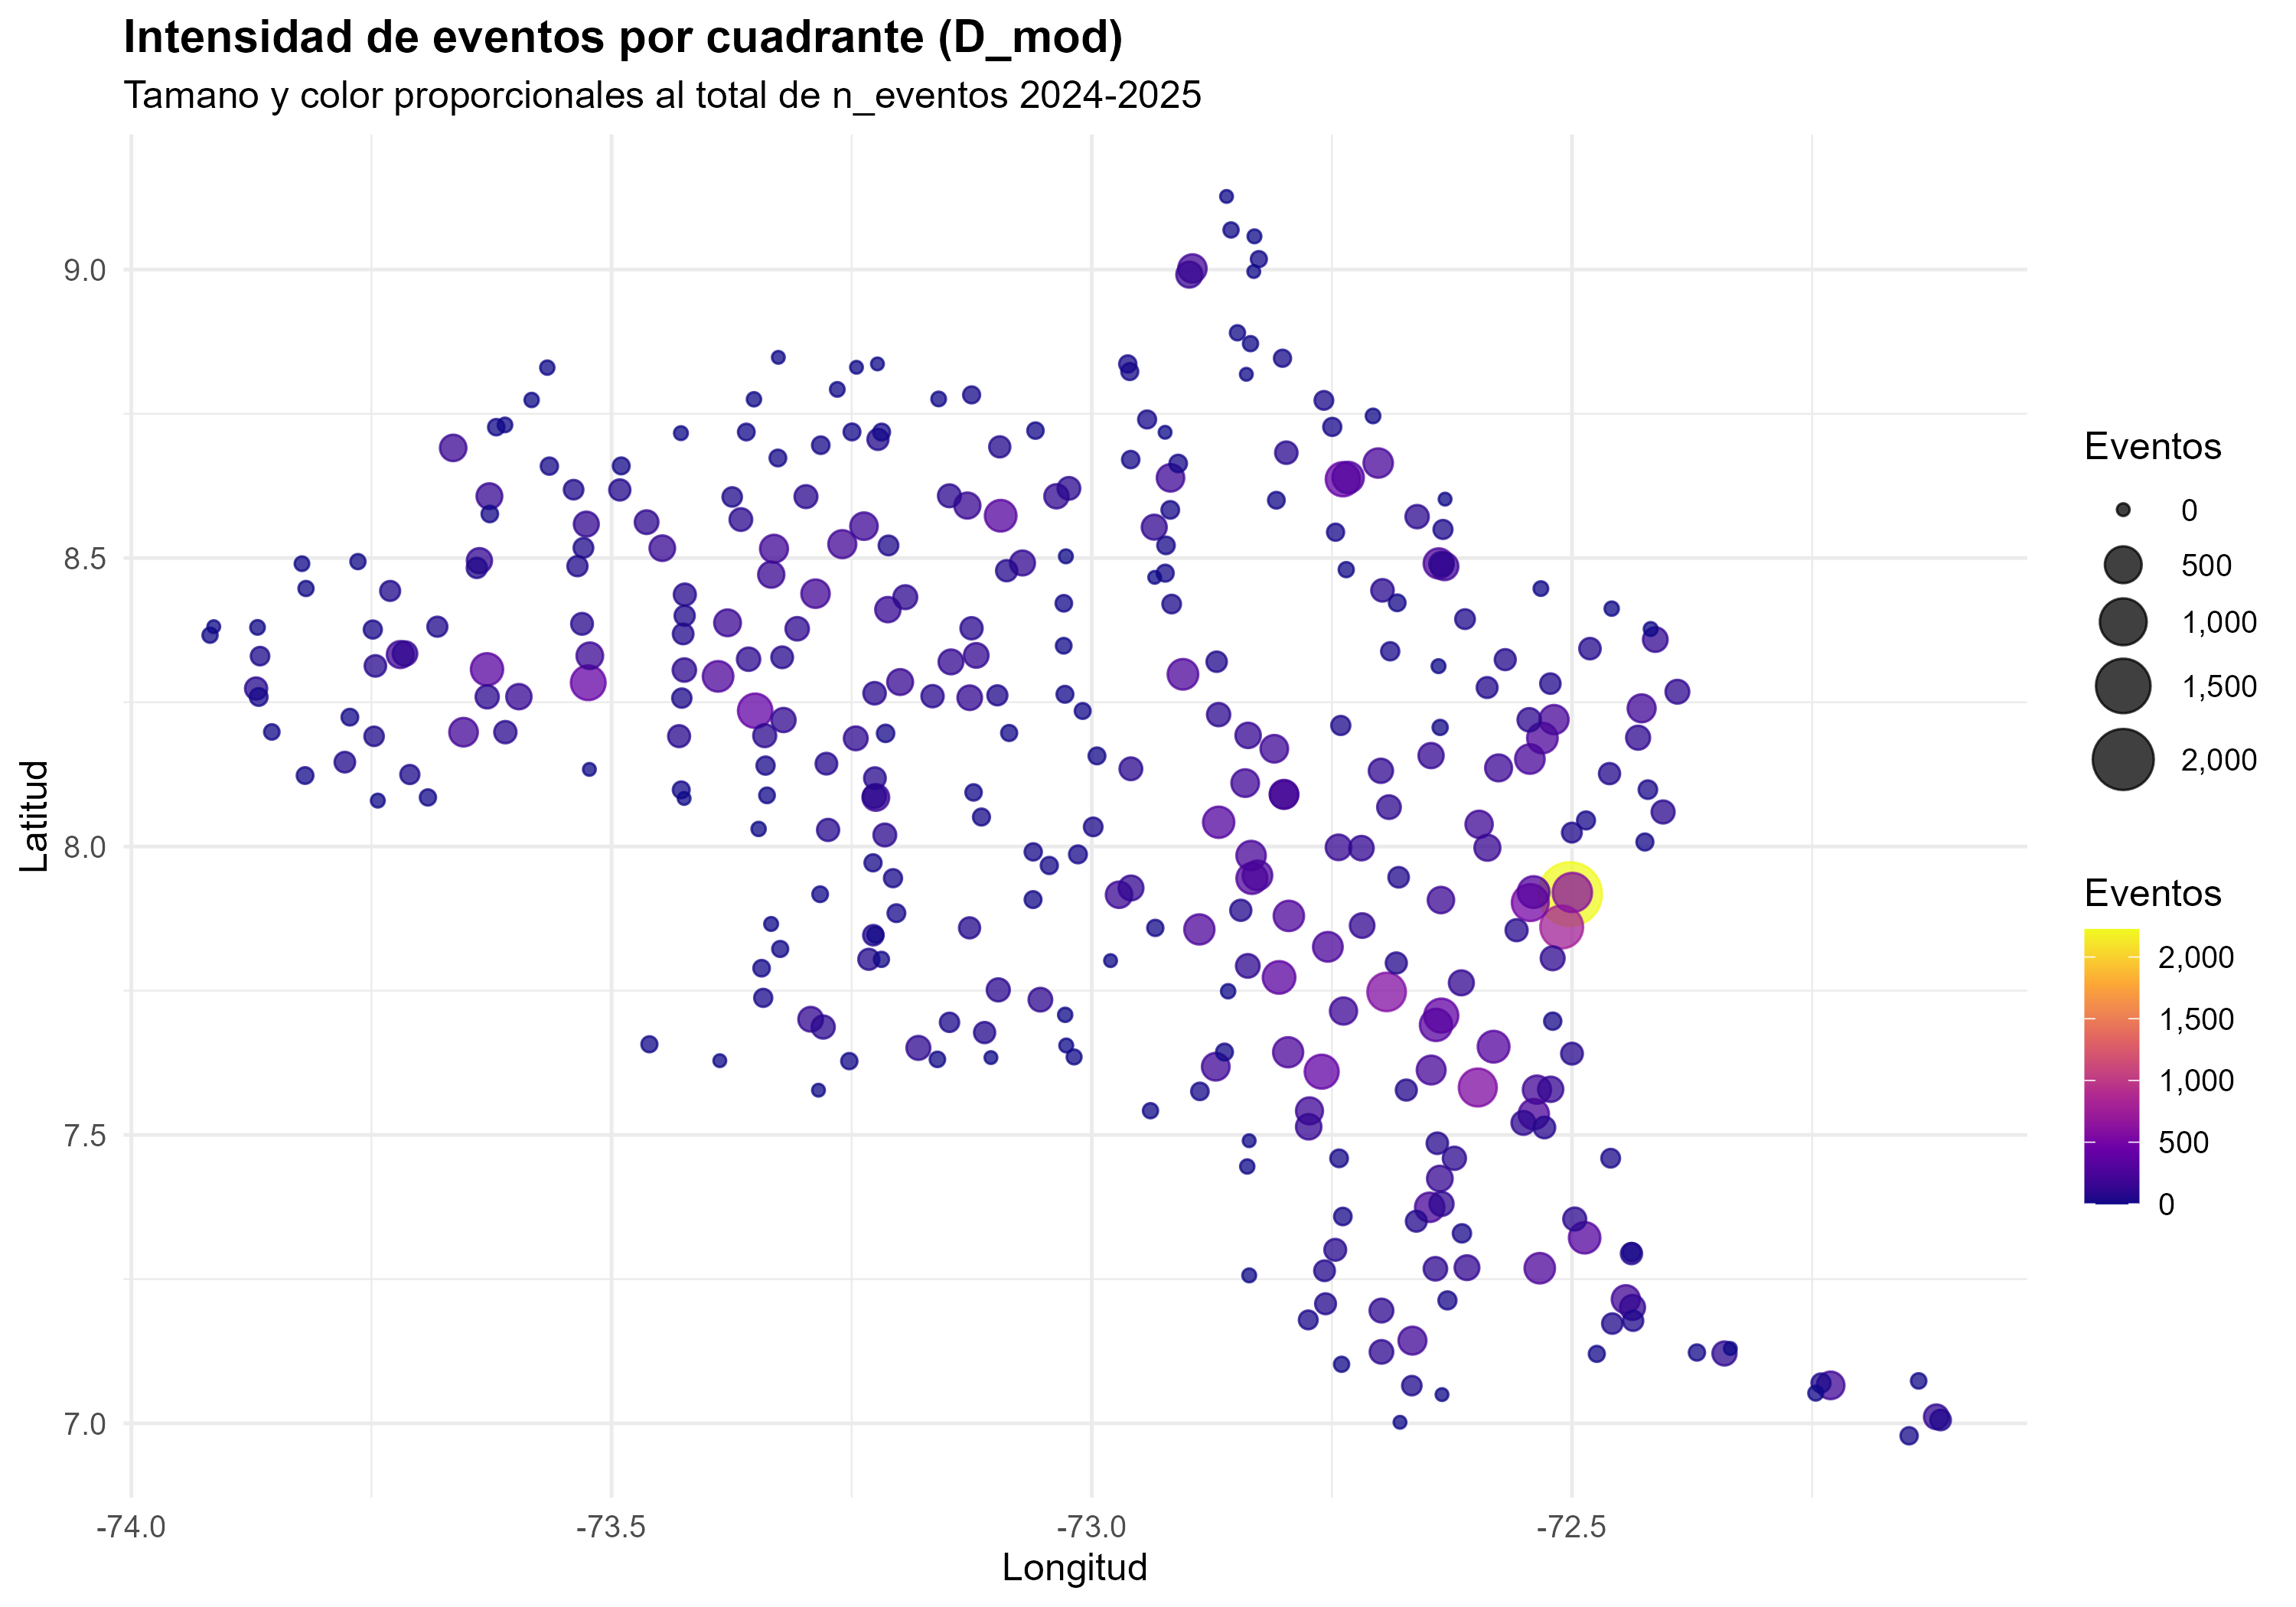
\includegraphics[width=0.90\textwidth]{img/mapa_intensidad_cuadrantes_patrones_mod.png}
        \caption{Intensidad territorial de eventos por cuadrante (2024--2025).}
        \label{fig:mapa_intensidad_mod}
    \end{figure}
    
    \paragraph{Patrones clima--evento.} Mediante la estimación de la correlación de Spearman a nivel cuadrante~$\times$~semana, las variables de viento exhiben la asociación positiva más fuerte con \texttt{n\_eventos} (\texttt{viento\_max\_semana}: $\hat{\rho} = 0{.}14$; \texttt{viento\_medio\_semana}: $\hat{\rho} = 0{.}14$; $p < 0{.}001$), seguidas de la precipitación acumulada semanal (\texttt{precip total semana}: $\hat{\rho} = 0{.}07$) y la humedad ($\hat{\rho} = 0{.}05$). La Figura~\ref{fig:dispersion_precip_mod} ilustra la relación entre precipitación y frecuencia de eventos: la nube muestra una tendencia positiva leve, sin un patrón fuerte. Las temperaturas presentan asociaciones débiles y negativas ($|\hat{\rho}| < 0{.}05$). En el grano semanal, por tanto, la señal climática es de magnitud modesta y está encabezada por el viento, no por la lluvia.

    
    \begin{figure}[!htbp]
        \centering
        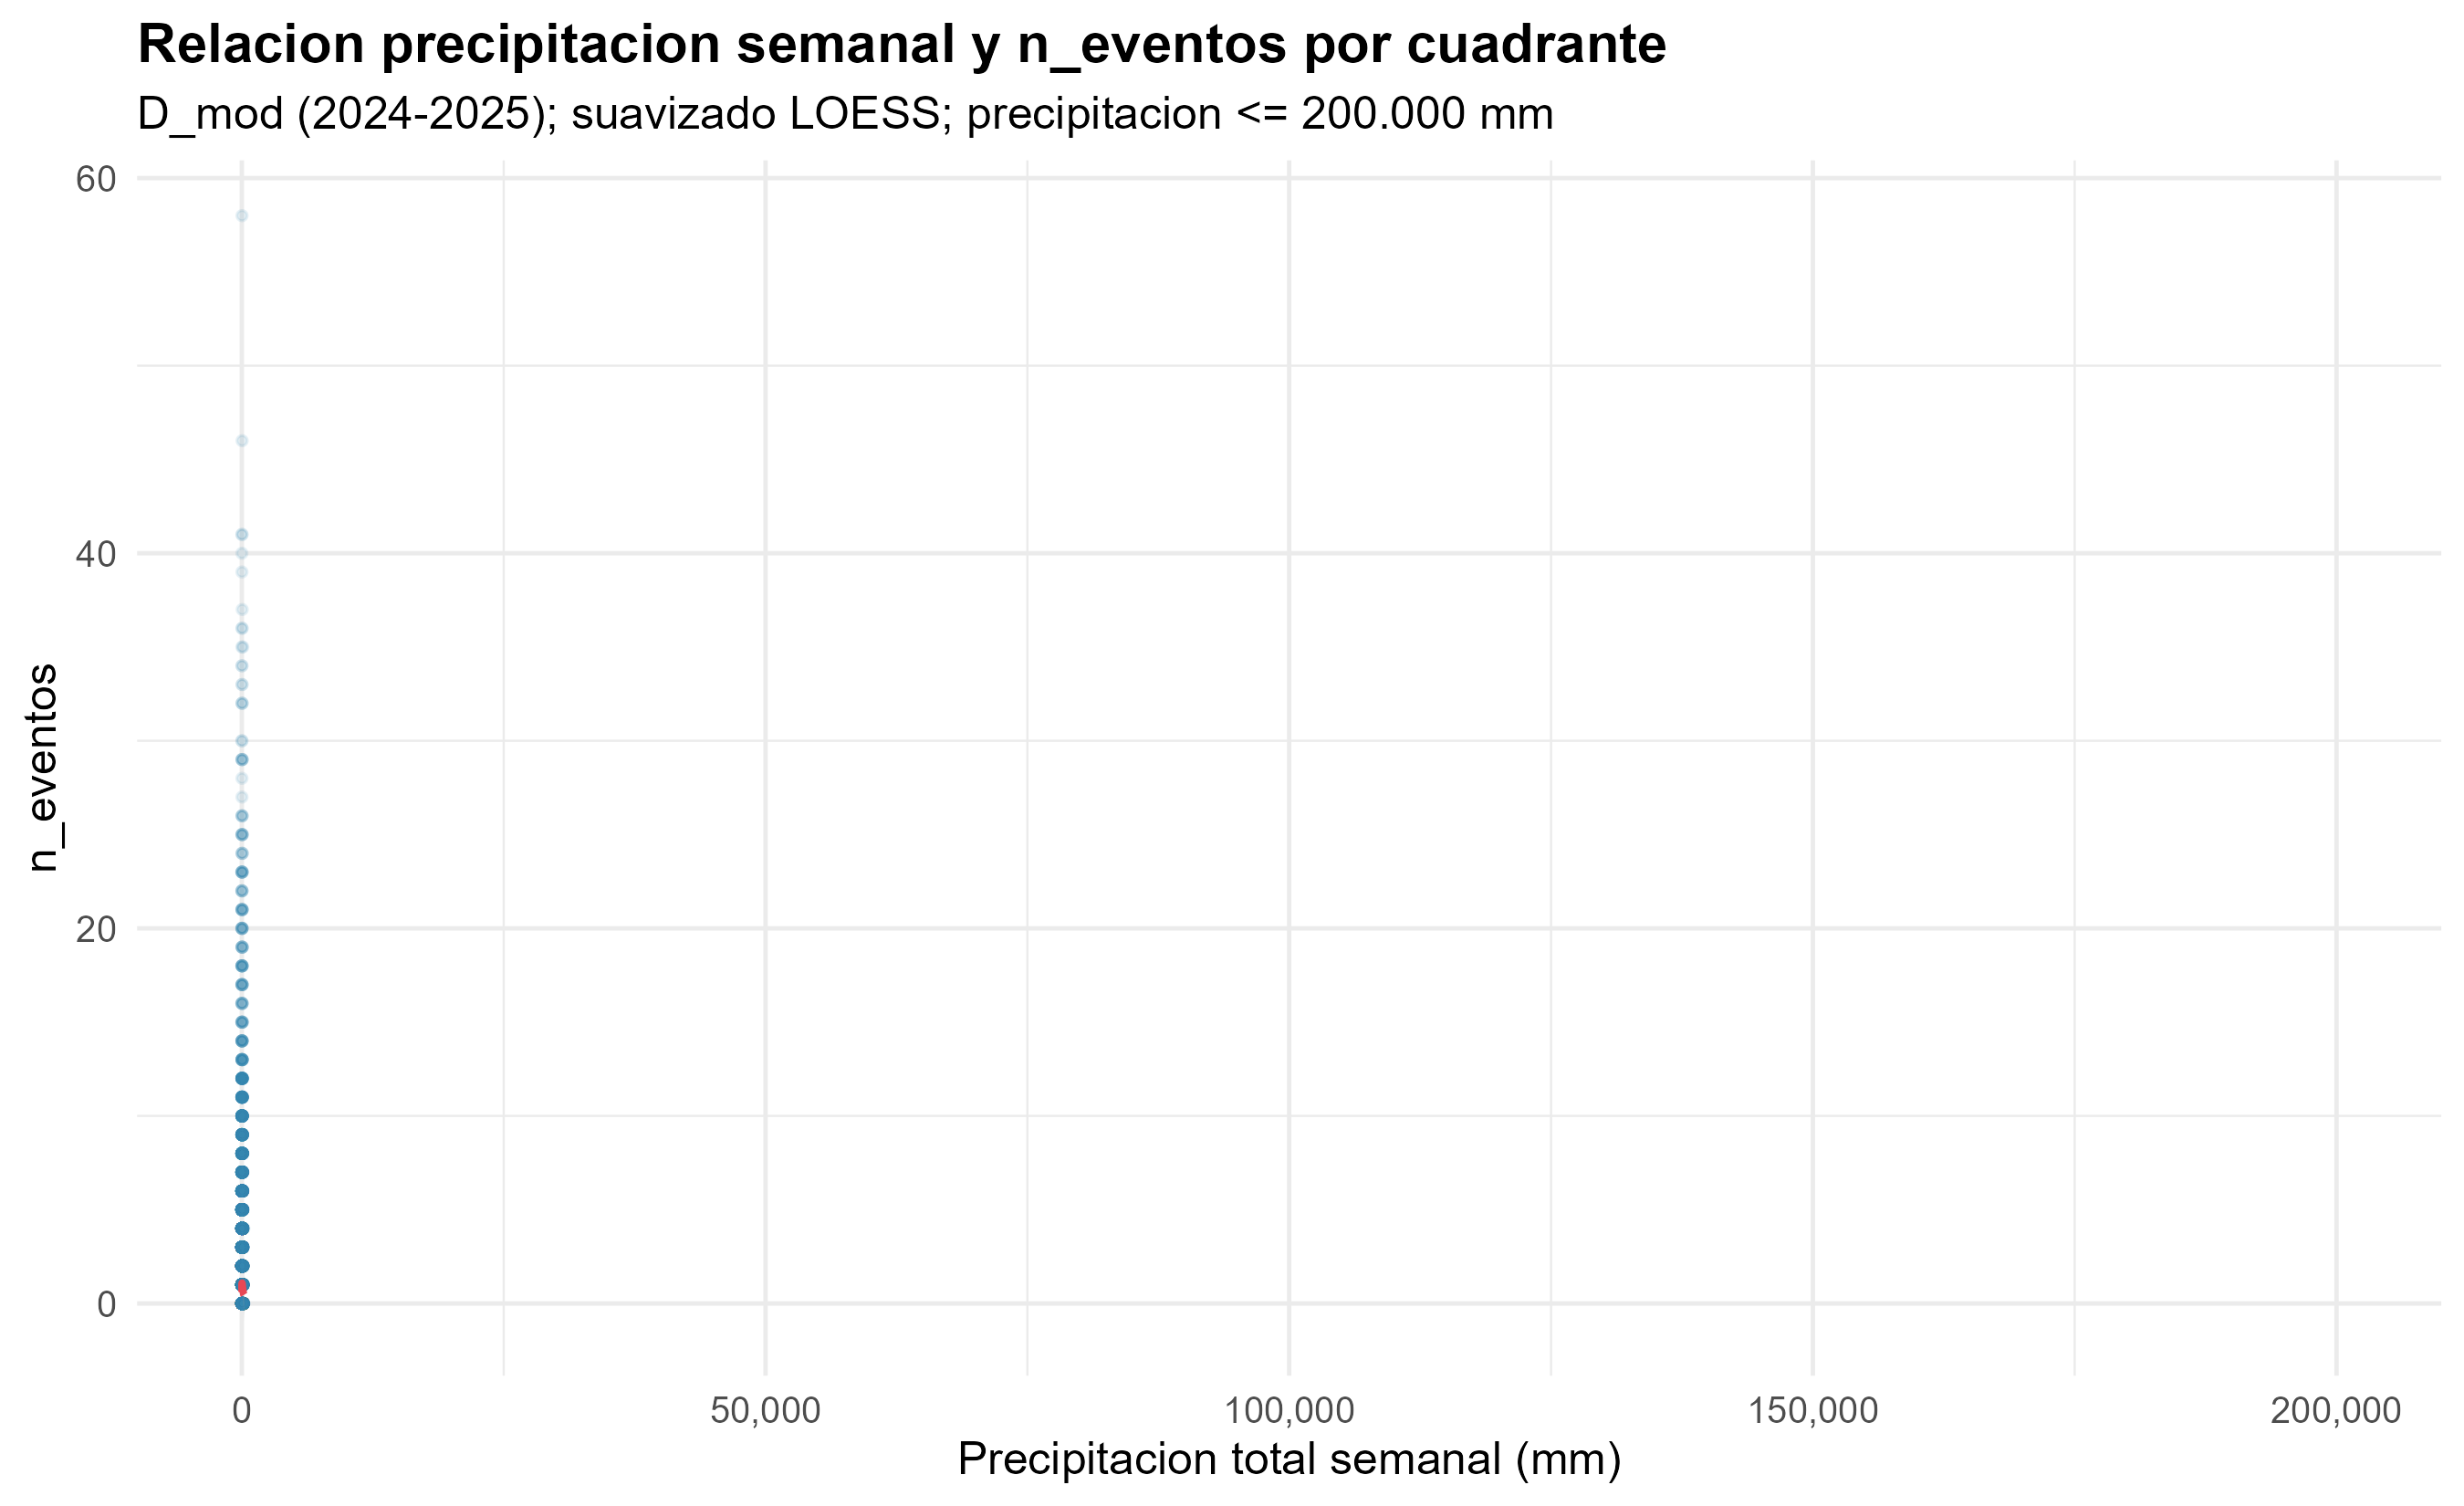
\includegraphics[width=0.85\textwidth]{img/dispersion_precip_eventos_patrones_mod.png}
        \caption{Relación entre precipitación semanal y frecuencia de eventos por cuadrante en $D_{\mathrm{mod}}$.}
        \label{fig:dispersion_precip_mod}
    \end{figure}
    
    \begin{figure}[!htbp]
        \centering
        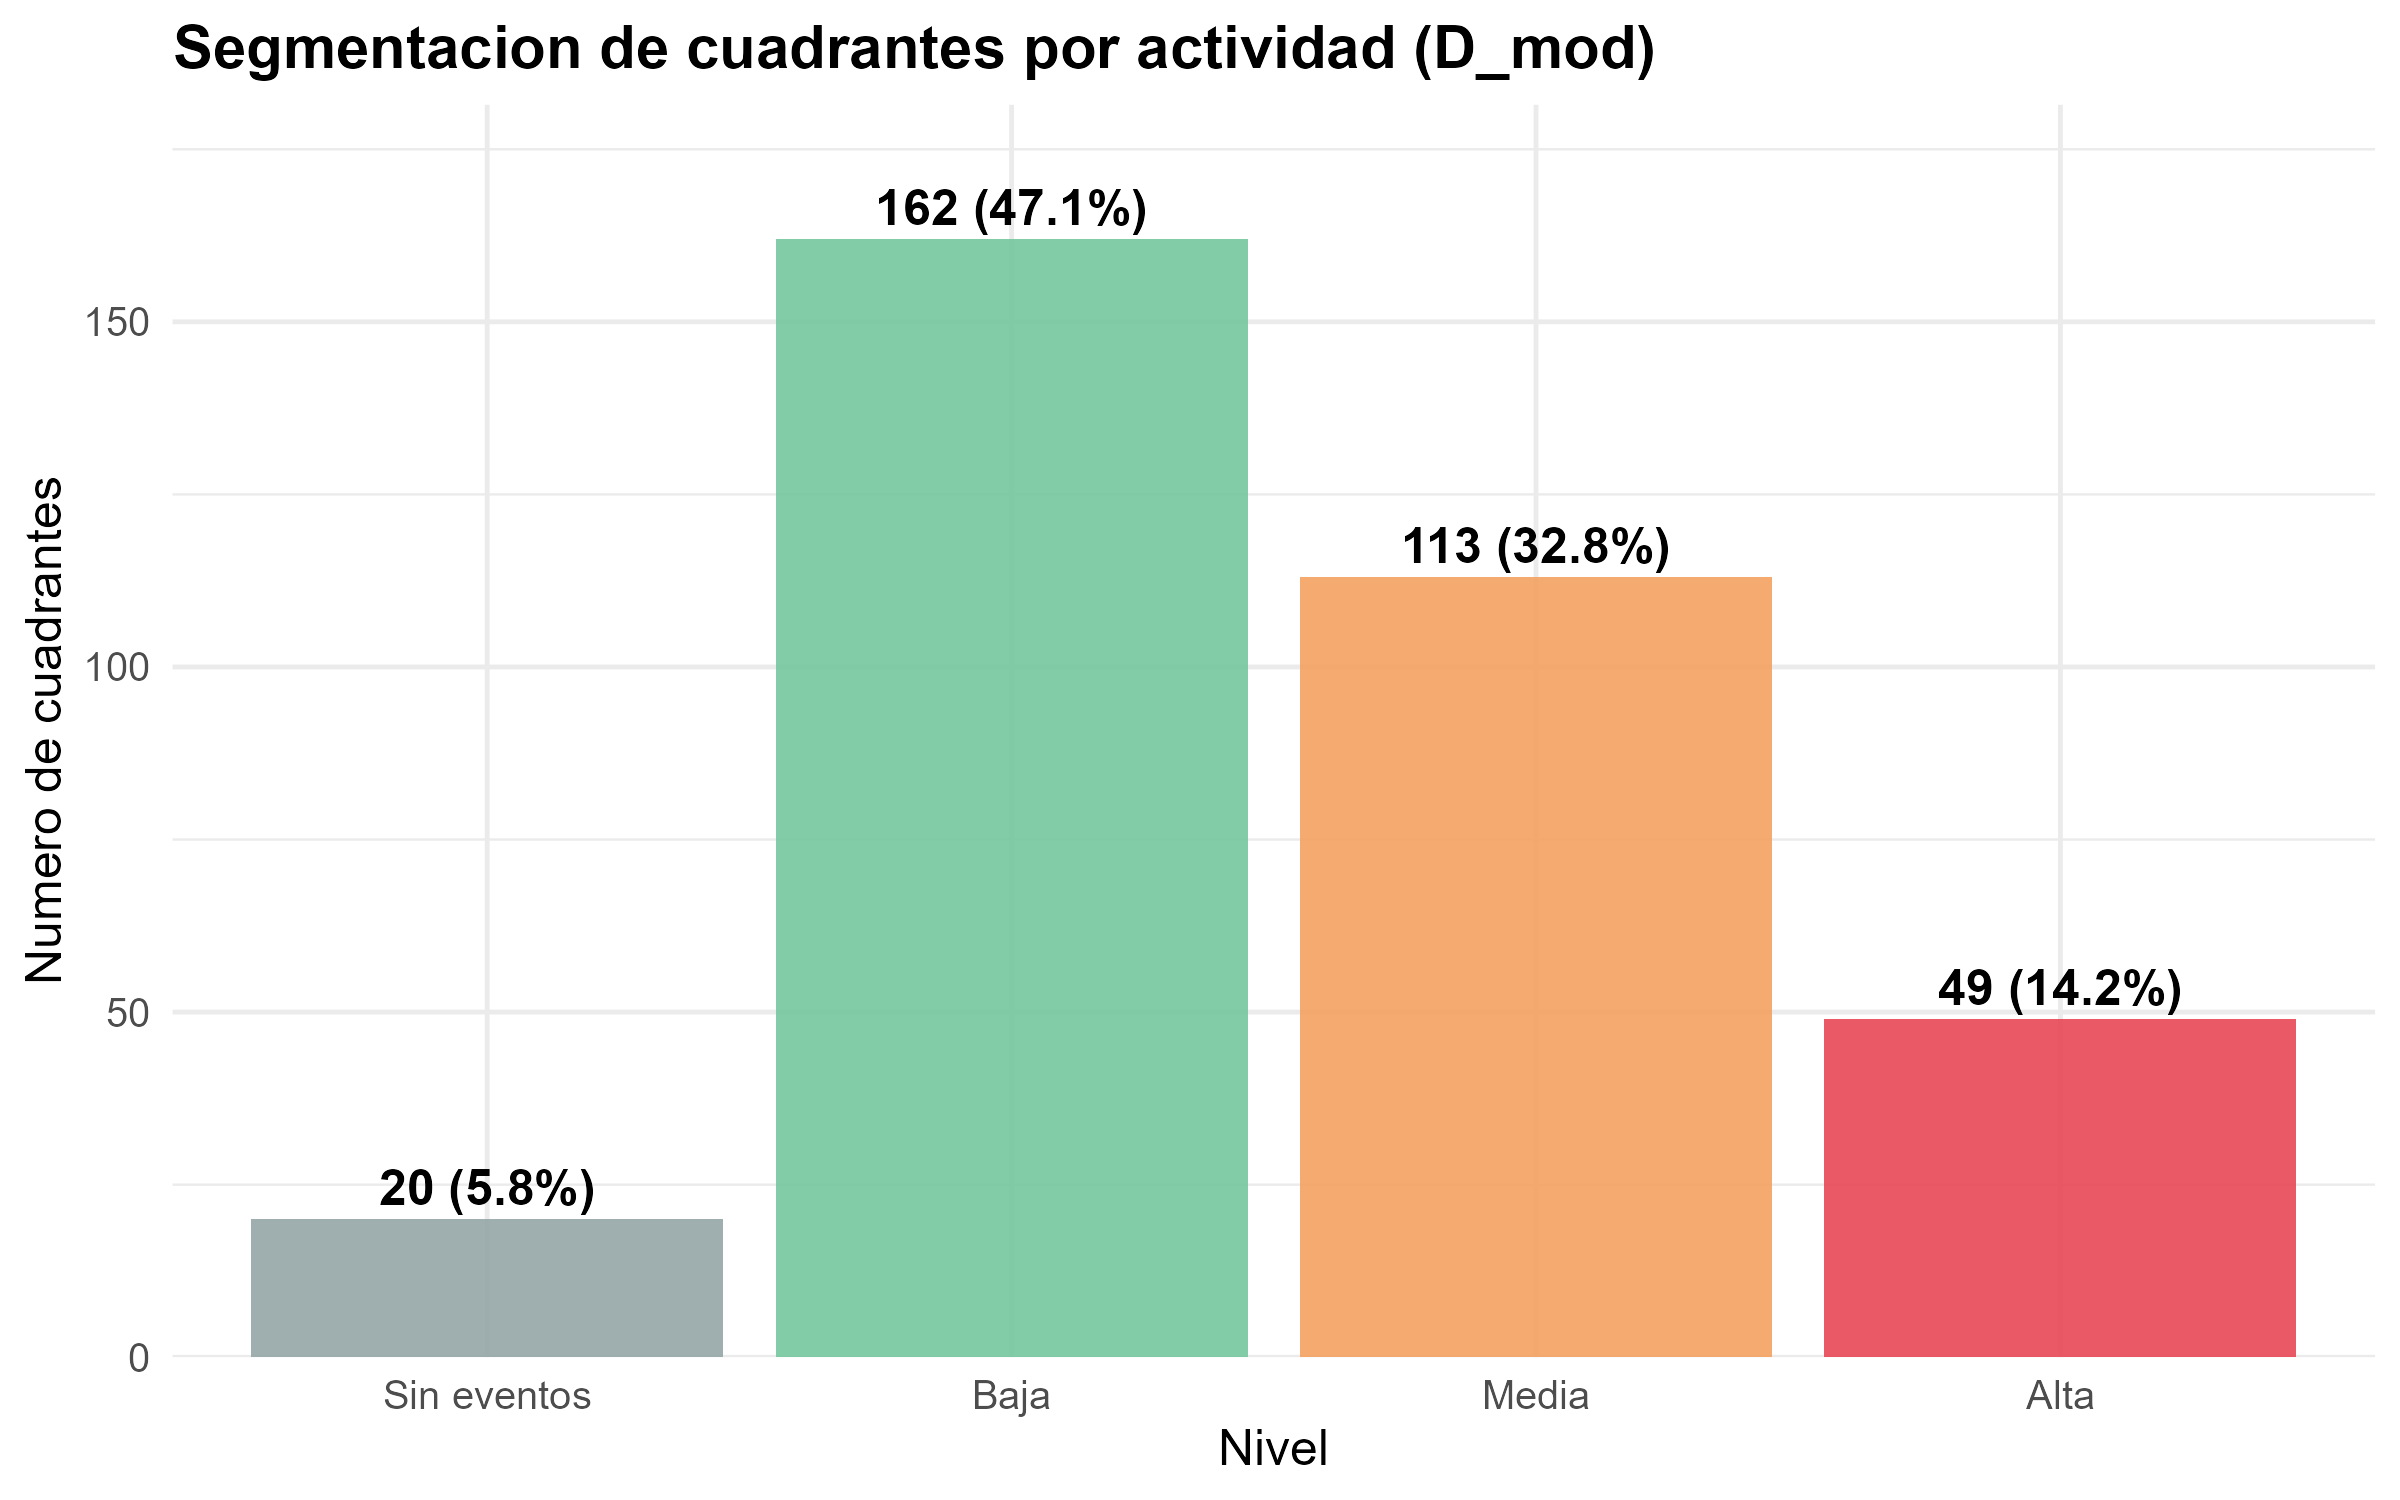
\includegraphics[width=0.75\textwidth]{img/segmentacion_cuadrantes_patrones_mod.png}
        \caption{Segmentación de cuadrantes por nivel de actividad acumulada en $D_{\mathrm{mod}}$.}
        \label{fig:segmentacion_mod}
    \end{figure}
    
    \noindent En síntesis, el análisis de patrones y la visualización exploratoria sobre $D_{\mathrm{mod}}$ confirman: (i)~persistencia y estacionalidad temporal (series semanales, estacionalidad mensual y ACF); (ii)~concentración espacial en un subconjunto de cuadrantes (ranking, mapa de intensidad y segmentación por actividad); y (iii)~asociación positiva pero débil entre las covariables meteorológicas y la frecuencia de interrupciones, encabezada por el viento y seguida por la precipitación (correlación de Spearman y diagrama de dispersión). Estos hallazgos orientan la selección de variables predictoras y la estratificación territorial de la Etapa~4. Los mapas de calor de correlaciones y el análisis multivariado formal se desarrollan en las Secciones~\ref{sec:analisis_correlacion_asociacion} y~\ref{sec:evaluacion_multivariada}.
    
\subsection{Análisis de correlación y asociación}
\label{sec:analisis_correlacion_asociacion}
    Con fundamento en los patrones preliminares de la Sección~\ref{sec:identificacion_patrones_tendencias}, se realizó un análisis sistemático de asociación pareada sobre \texttt{data\_agrupada\_mod.csv} ($D_{\mathrm{mod}}$; $36\,120$ filas cuadrante~$\times$~semana). Dado el carácter asimétrico, cero-inflado y de colas pesadas de las variables operativas (Sección~\ref{sec:distribucion_variables}), se empleó el coeficiente de correlación de \textit{Spearman} en lugar de Pearson. El procedimiento reproducible se documenta en el Apéndice~\ref{app:html-correlacion}.
    
    \paragraph{Matriz de asociación global.} Se calcularon las correlaciones de Spearman entre las variables operativas (\texttt{n\_eventos}, \texttt{usuarios\_afectados}, \texttt{elementos\_afectados}, \texttt{duracion\_total}), las siete variables climáticas semanales y las coordenadas geográficas (\texttt{altitud}, \texttt{latitud}, \texttt{longitud}). La Figura~\ref{fig:heatmap_cor_clima_operativo} resume la submatriz clima--operativo. Los pares con mayor asociación absoluta del panel completo concentran redundancia operativa: \texttt{usuarios\_afectados}--\texttt{elementos\_afectados} ($\rho = 0{.}99$), \texttt{n\_eventos}--\texttt{elementos\_afectados} ($\rho = 0{.}98$) y \texttt{n\_eventos}--\texttt{usuarios\_afectados} ($\rho = 0{.}97$). Parte de esta magnitud es \textit{mecánica}: las tres métricas provienen de la misma tabla de eventos, comparten la masa de ceros en semanas sin interrupción y, al agregarse por suma, crecen juntas cuando aumenta el número de eventos. Por ello no deben interpretarse como evidencia de tres dimensiones independientes ni usarse simultáneamente como respuesta y predictoras; la definición definitiva del rol de la severidad se aplaza a la Etapa~4.
    
    \begin{figure}[!htbp]
        \centering
        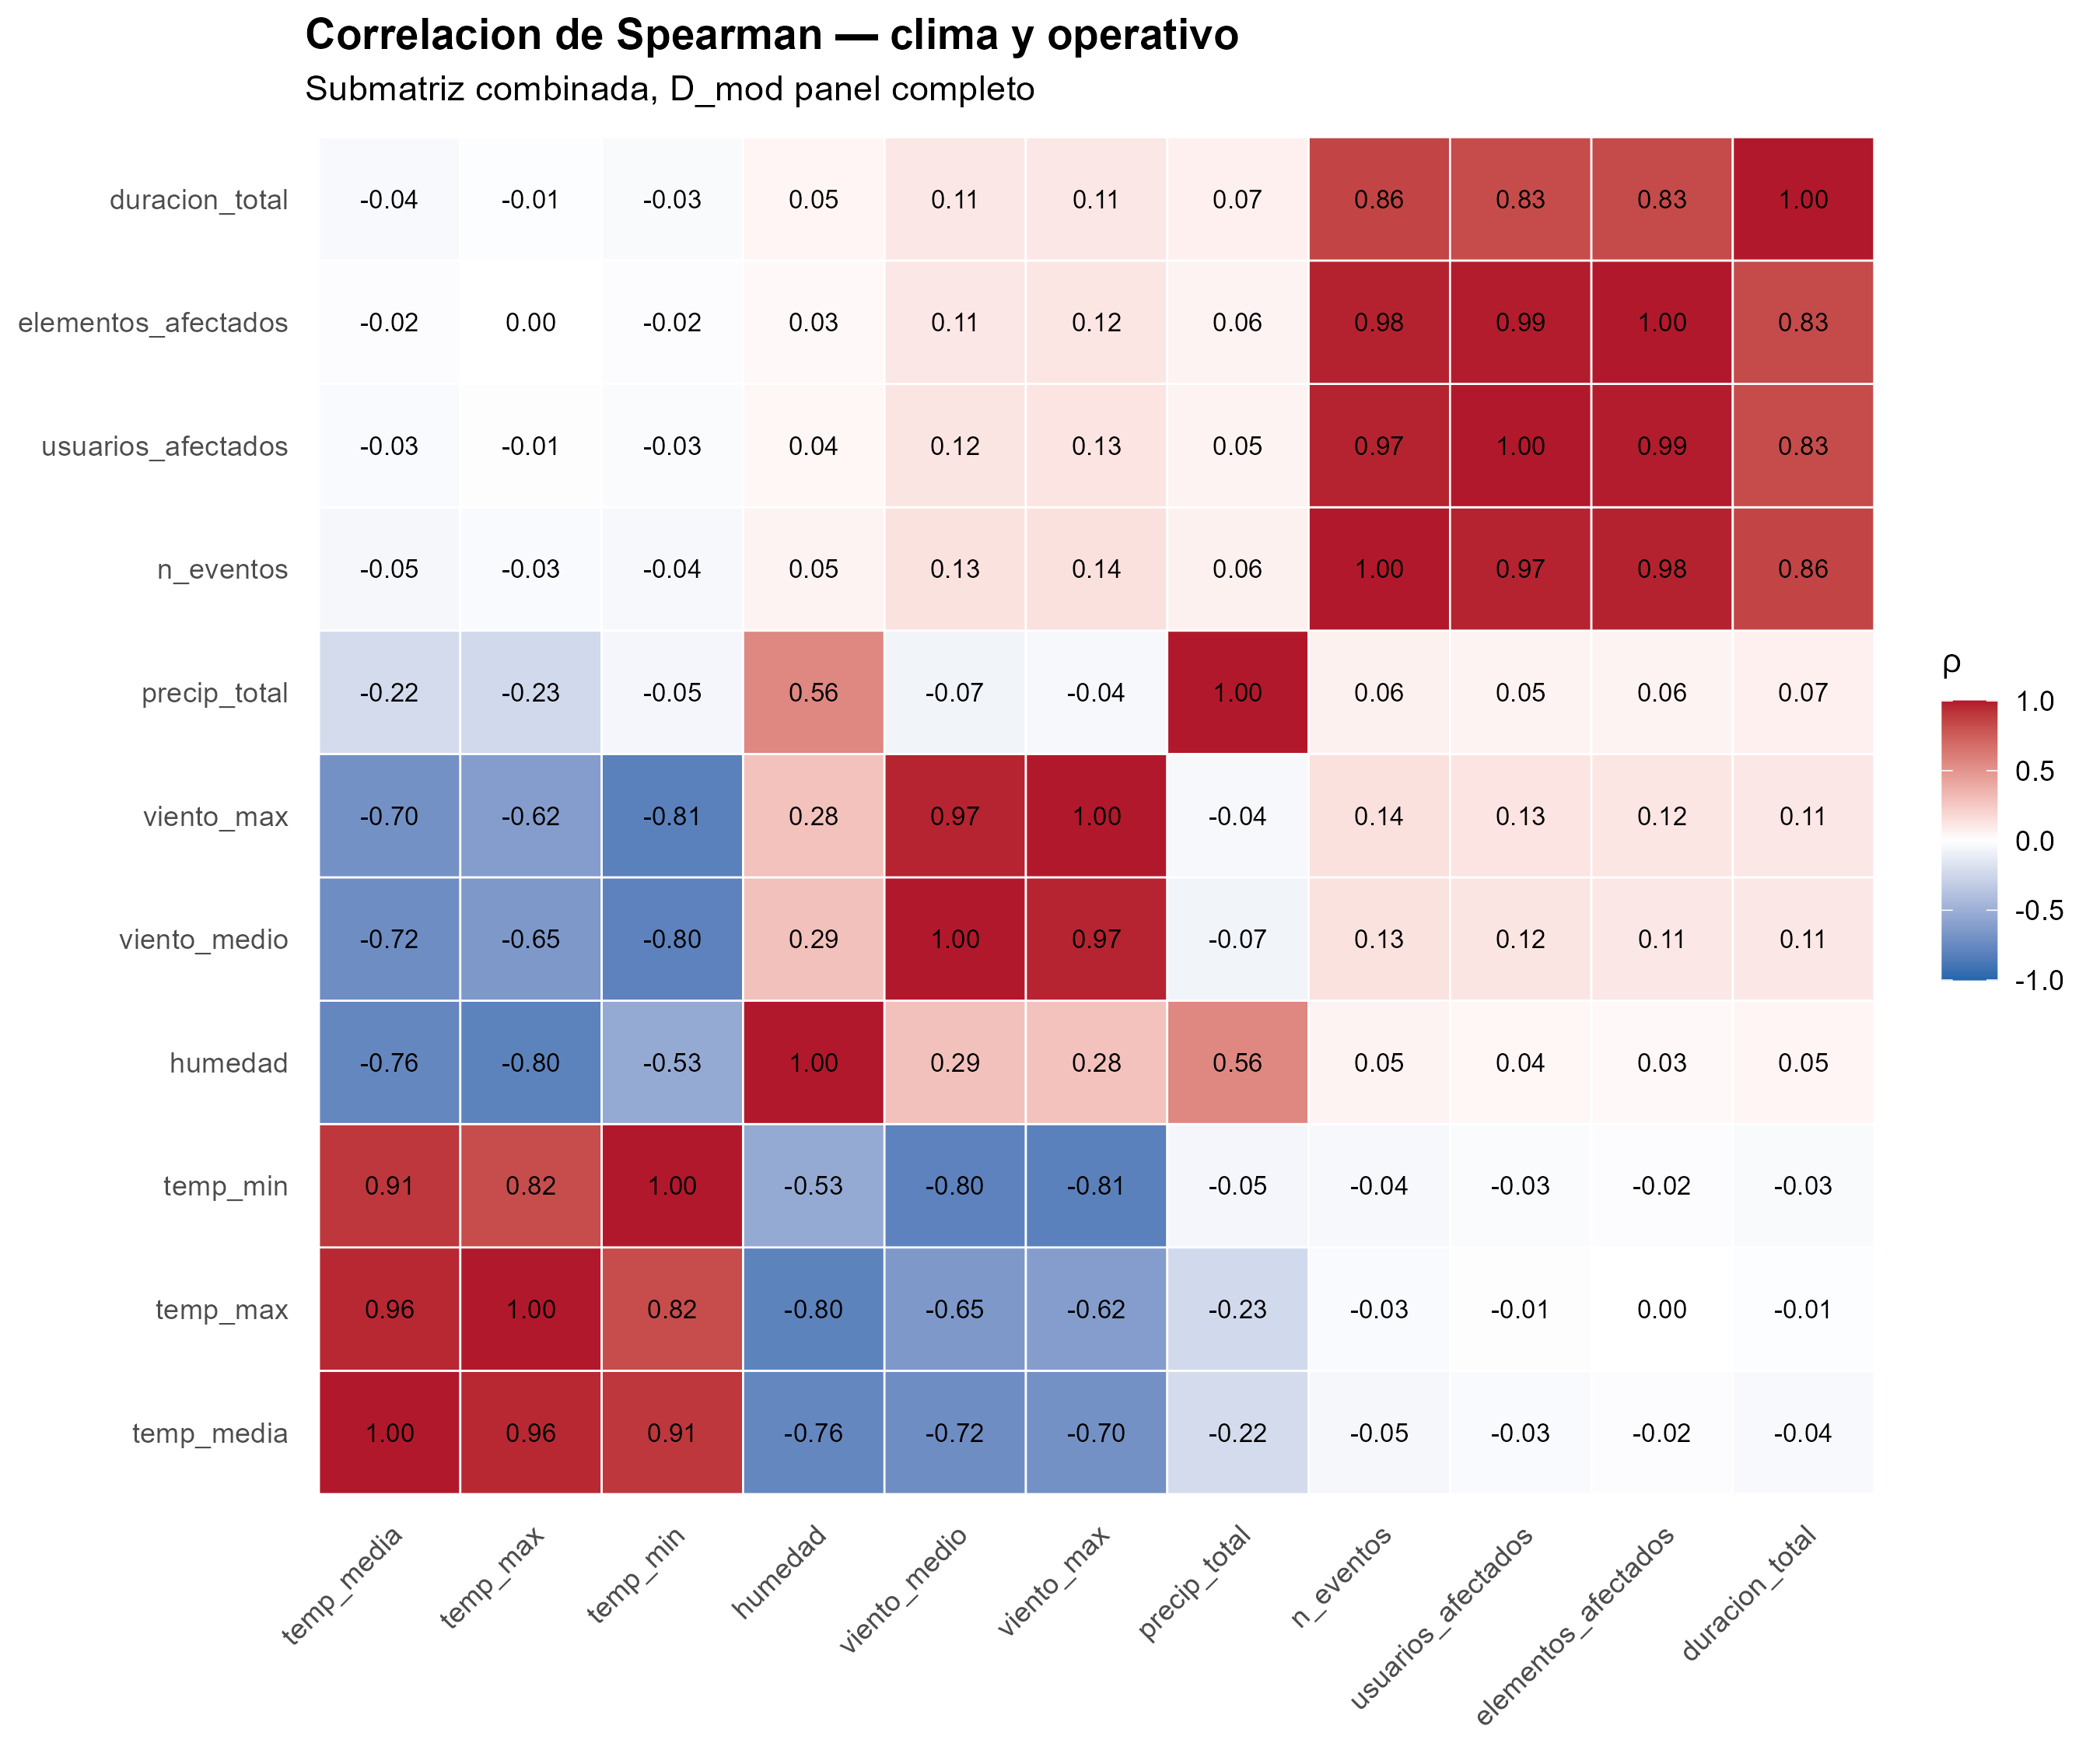
\includegraphics[width=0.92\textwidth]{img/heatmap_correlacion_clima_operativo_mod.png}
        \caption{Asociación de Spearman entre variables climáticas y operativas en $D_{\mathrm{mod}}$.}
        \label{fig:heatmap_cor_clima_operativo}
    \end{figure}
    
    \paragraph{Bloque climático: redundancias.} En el bloque meteorológico (Figura~\ref{fig:heatmap_cor_clima}) se identificaron \textit{diez} pares con $|\rho| \geq 0{.}70$, principalmente entre temperaturas (\texttt{temp\_media}--\texttt{temp\_max}: $\rho = 0{.}96$; \texttt{temp\_media}--\texttt{temp\_min}: $\rho = 0{.}91$) y entre componentes de viento ($\rho = 0{.}97$). Las temperaturas presentan además asociación negativa moderada con la humedad ($\rho \approx -0{.}76$ a $-0{.}80$) y con el viento ($\rho \approx -0{.}70$ a $-0{.}81$). La precipitación no participa en ninguno de estos pares: su mayor asociación dentro del bloque queda por debajo del umbral, lo que la señala como la única covariable climática no redundante. Estos resultados anticipan \textit{multicolinealidad} entre temperaturas y vientos, y orientan la depuración de variables en la Etapa~4.
    
    \begin{figure}[!htbp]
        \centering
        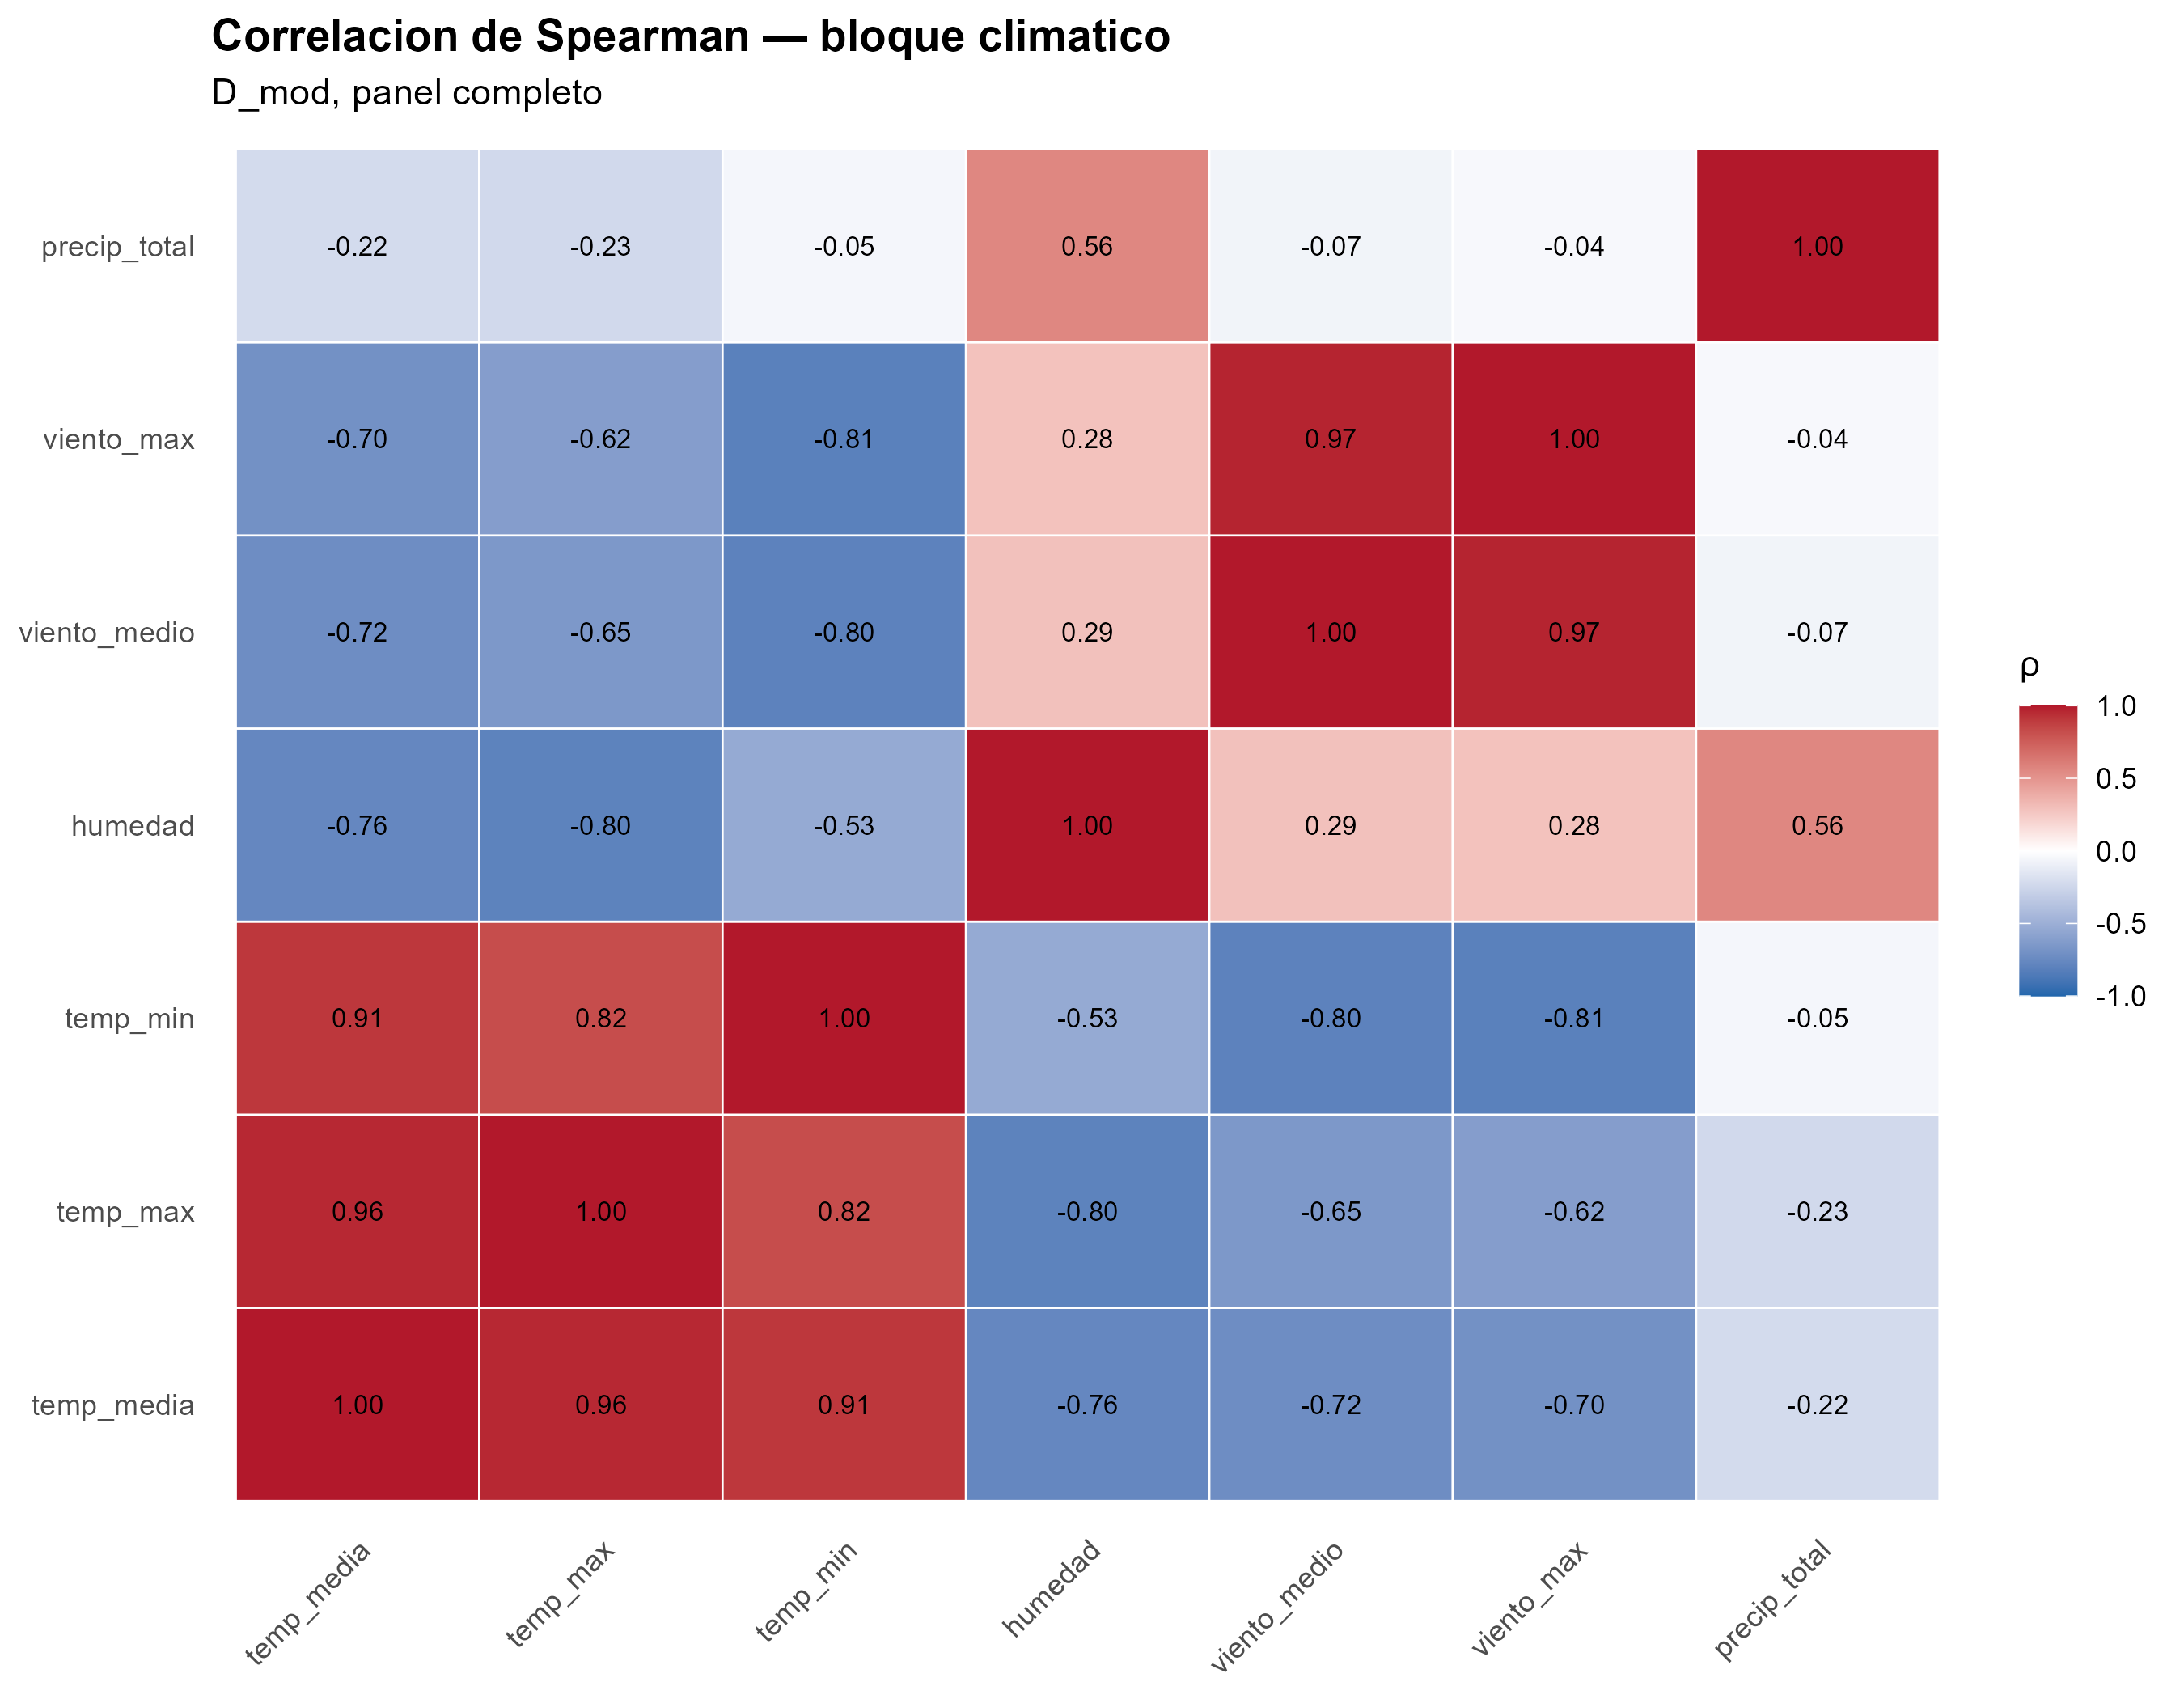
\includegraphics[width=0.85\textwidth]{img/heatmap_correlacion_clima_mod.png}
        \caption{Correlaciones de Spearman en el bloque climático semanal ($D_{\mathrm{mod}}$).}
        \label{fig:heatmap_cor_clima}
    \end{figure}
    
    \paragraph{Bloque operativo.} La Figura~\ref{fig:heatmap_cor_operativo} muestra que las cuatro métricas de continuidad y severidad están fuertemente correlacionadas entre sí ($\rho$ entre $0{.}83$ y $0{.}99$), aunque \texttt{duracion\_total} exhibe una asociación algo menor con \texttt{n\_eventos} ($\rho = 0{.}86$) que con las variables de afectación. Frecuencia y duración capturan dimensiones parcialmente distintas; el alcance (\texttt{usuarios\_afectados}, \texttt{elementos\_afectados}) queda, en esta construcción, muy alineado con la frecuencia y se trata aquí como diagnóstico exploratorio de severidad, no como predictor independiente.
    
    \begin{figure}[!htbp]
        \centering
        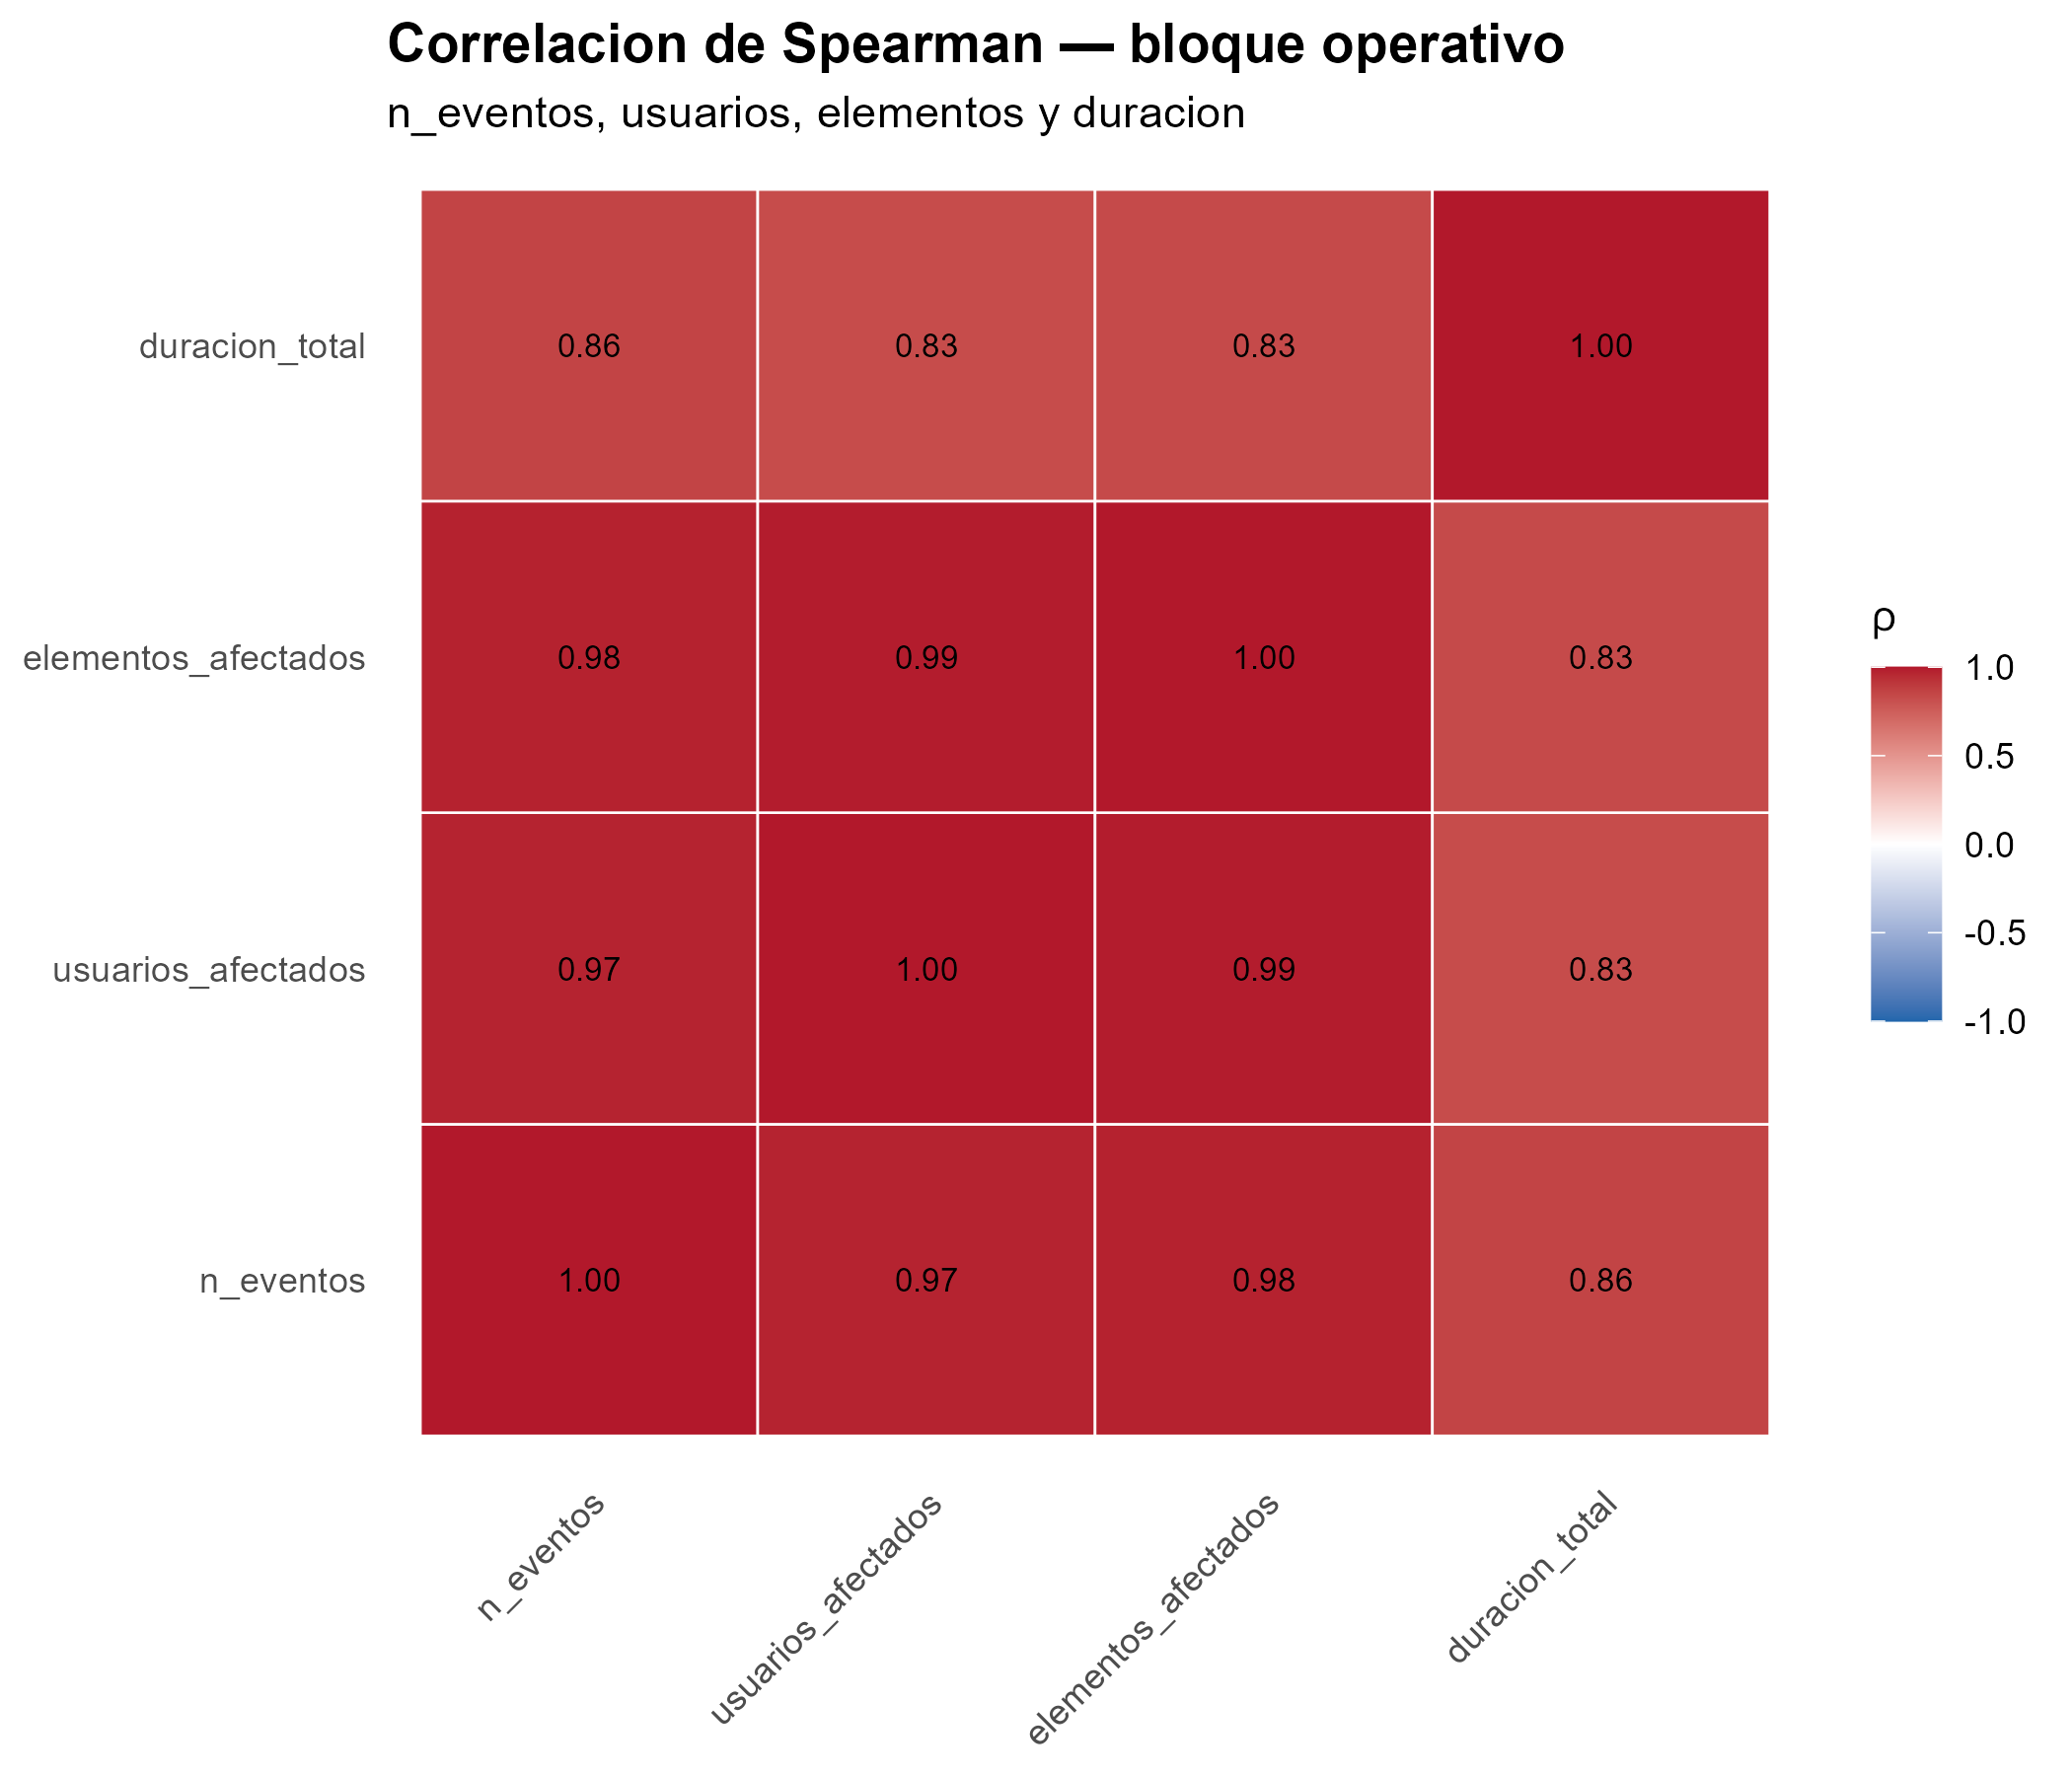
\includegraphics[width=0.72\textwidth]{img/heatmap_correlacion_operativo_mod.png}
        \caption{Correlaciones de Spearman entre variables operativas en $D_{\mathrm{mod}}$.}
        \label{fig:heatmap_cor_operativo}
    \end{figure}
    
    \paragraph{Clima $\rightarrow$ operativo.} La Figura~\ref{fig:barras_cor_clima_operativo} y la Tabla~\ref{tab:clima_operativo_cor} cuantifican la asociación entre covariables meteorológicas y métricas de interrupción. Todas las asociaciones son estadísticamente significativas, consecuencia esperable del tamaño del panel, pero de magnitud pequeña. Las variables de \textit{viento} encabezan el bloque: \texttt{viento\_max\_semana} con \texttt{n\_eventos} ($\rho = 0{.}139$) y \texttt{viento\_medio\_semana} con \texttt{n\_eventos} ($\rho = 0{.}135$), con valores del mismo orden frente a \texttt{usuarios\_afectados} ($\rho \approx 0{.}12$), \texttt{elementos\_afectados} ($\rho \approx 0{.}11$) y \texttt{duracion\_total} ($\rho \approx 0{.}11$). La \texttt{precip\_total\_semana} le sigue con asociaciones positivas débiles ($\rho = 0{.}069$ con \texttt{duracion\_total} y $\rho = 0{.}065$ con \texttt{n\_eventos}), mientras la humedad ($\rho \approx 0{.}05$) y las temperaturas ($|\rho| < 0{.}05$, con signo negativo) resultan prácticamente irrelevantes en el grano semanal.

    Conviene precisar el alcance de este resultado. La magnitud reducida de la asociación no implica ausencia de efecto físico de la lluvia sobre la red, sino que el acumulado semanal por cuadrante es un descriptor grueso del fenómeno: promedia días secos y días de tormenta, y no captura la intensidad horaria ni la coincidencia temporal exacta entre el evento meteorológico y la desconexión. Con este descriptor, la asociación bivariada disponible en el grano cuadrante~$\times$~semana es débil, y así se reporta.
    
    \begin{figure}[!htbp]
        \centering
        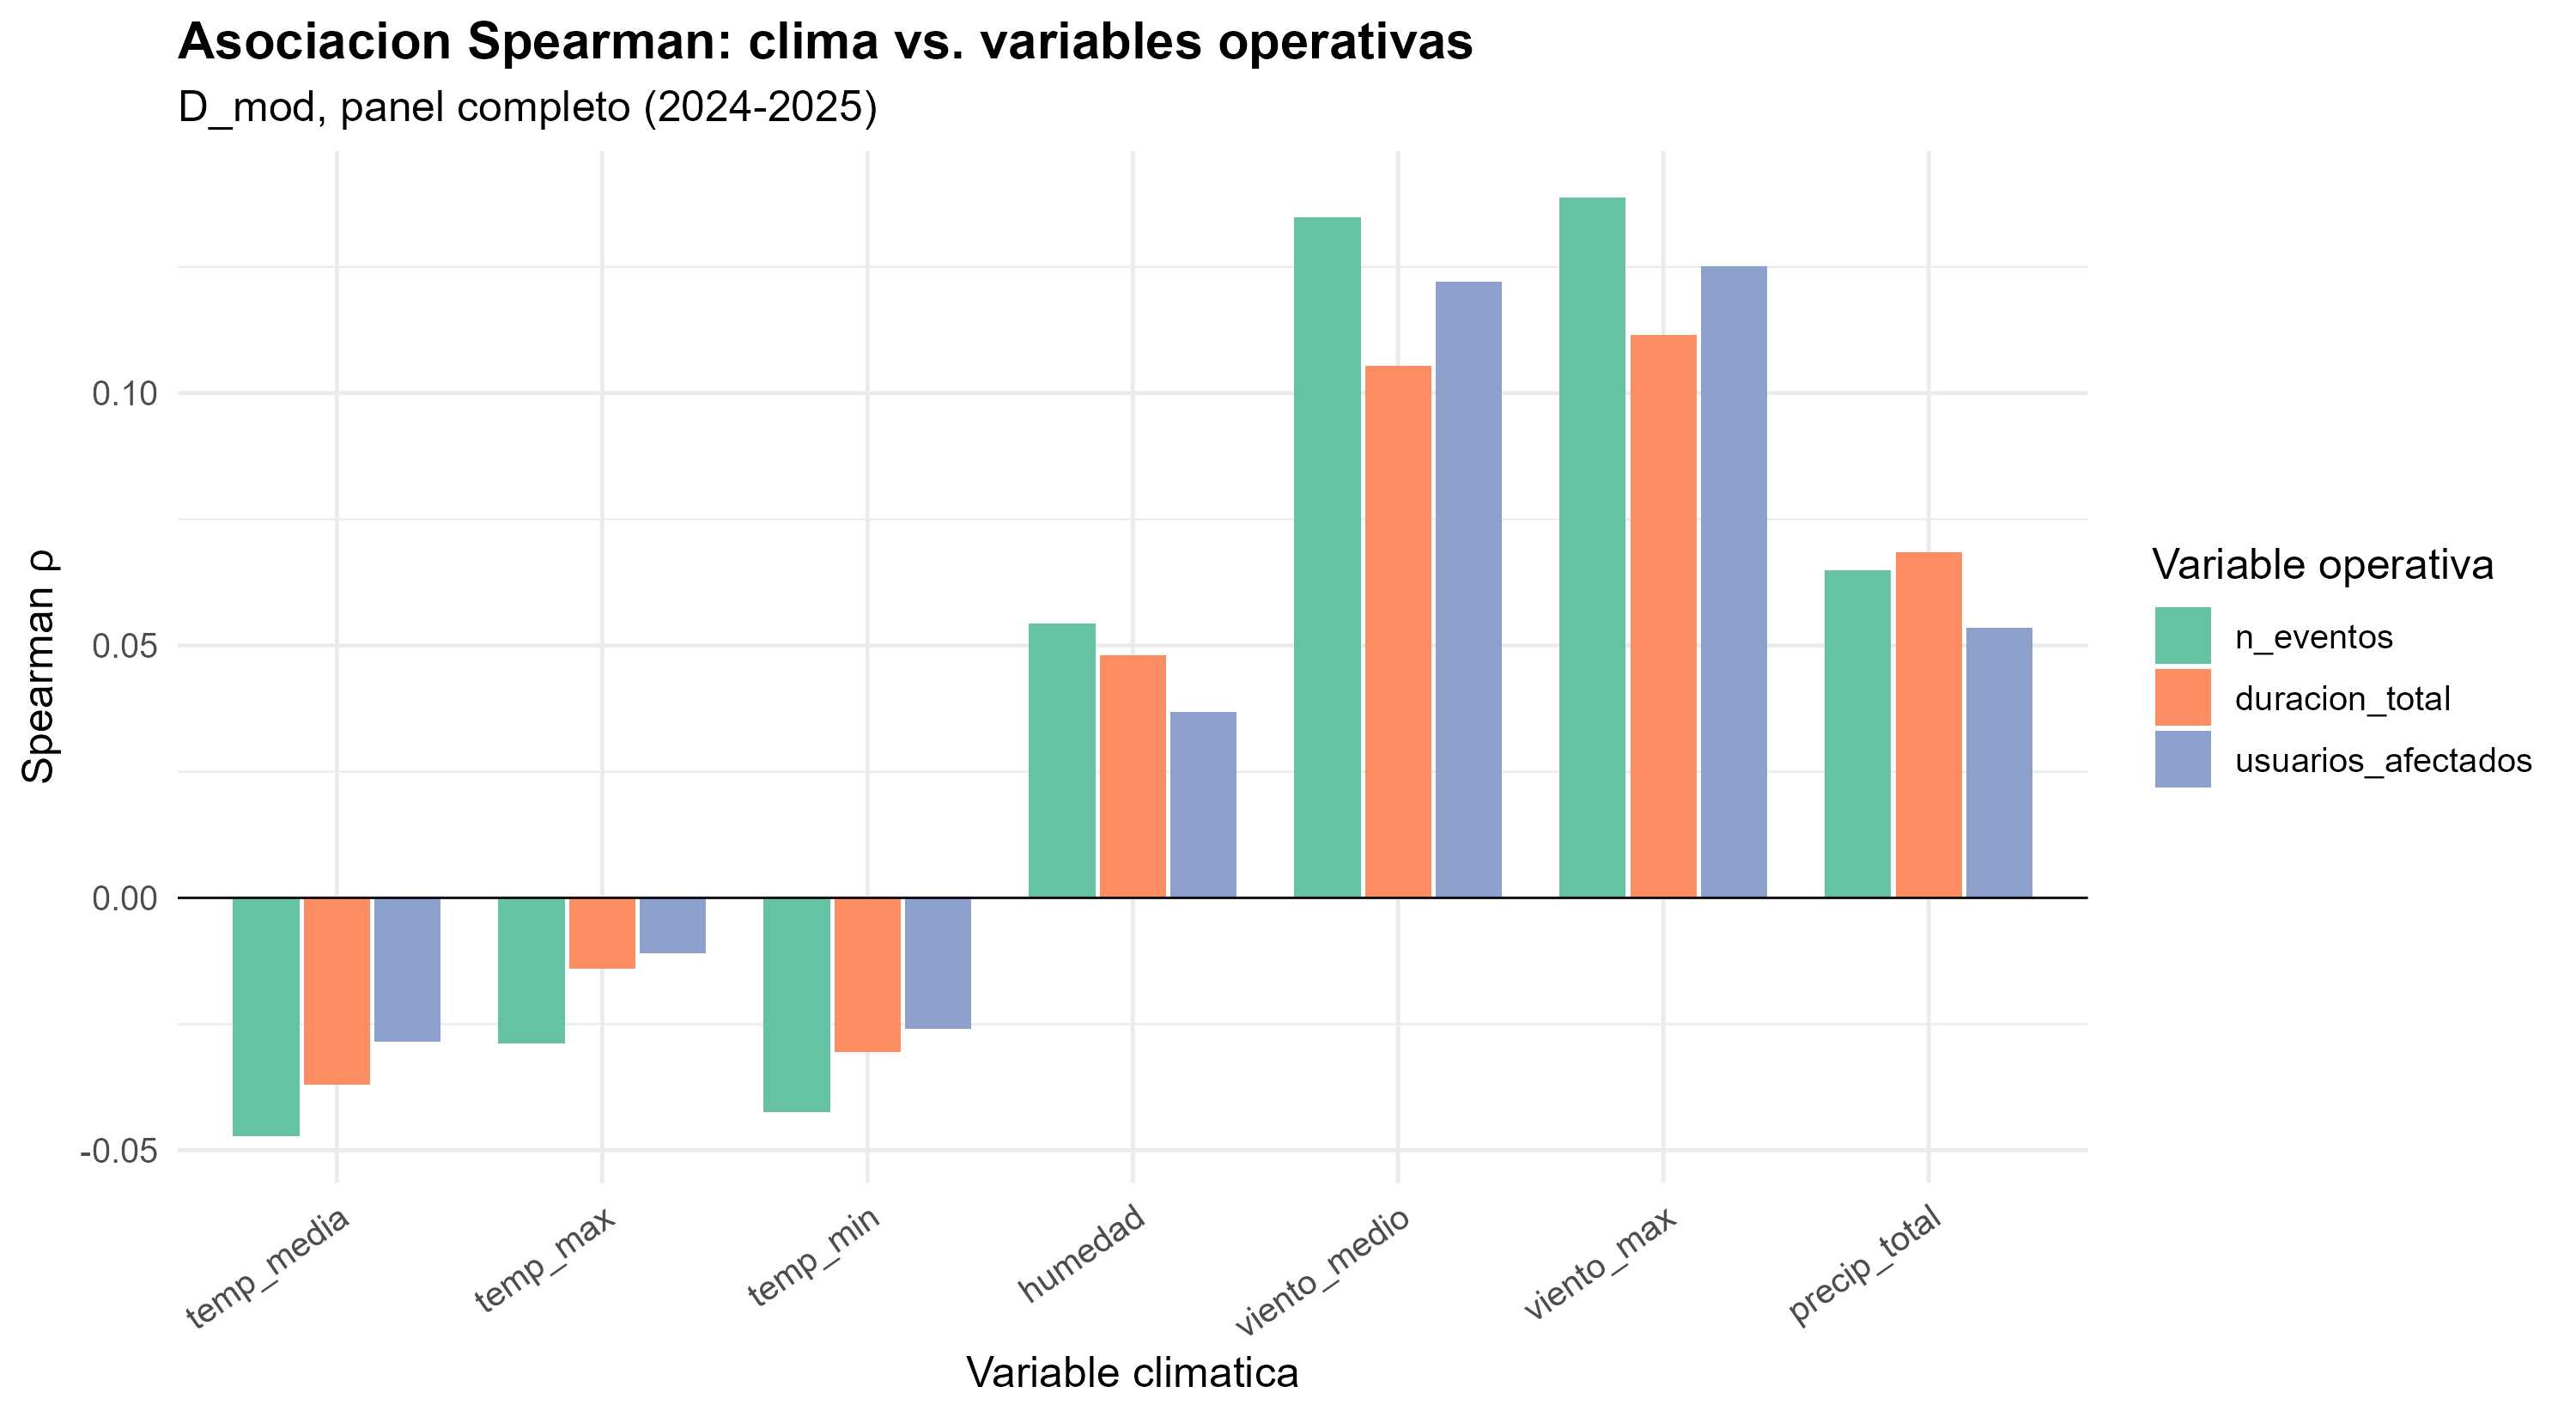
\includegraphics[width=0.95\textwidth]{img/barras_correlacion_clima_operativo_mod.png}
        \caption{Coeficientes de Spearman entre variables climáticas y operativas en $D_{\mathrm{mod}}$.}
        \label{fig:barras_cor_clima_operativo}
    \end{figure}
    
    \begin{table}[!htbp]
    \centering
    \small
    \caption{Asociación Spearman entre clima y variables operativas: pares de mayor magnitud ($D_{\mathrm{mod}}$; panel completo)}
    \label{tab:clima_operativo_cor}
    \begin{tabular}{@{}l r r@{}}
    \toprule
    \textbf{Par de variables} & \textbf{Spearman $\rho$} & \textbf{$p$-valor} \\
    \midrule
    \texttt{viento\_max\_semana} $\leftrightarrow$ \texttt{n\_eventos}            & 0.139 & $< 0{.}001$ \\
    \texttt{viento\_medio\_semana} $\leftrightarrow$ \texttt{n\_eventos}           & 0.135 & $< 0{.}001$ \\
    \texttt{viento\_max\_semana} $\leftrightarrow$ \texttt{usuarios\_afectados}    & 0.125 & $< 0{.}001$ \\
    \texttt{viento\_max\_semana} $\leftrightarrow$ \texttt{duracion\_total}        & 0.112 & $< 0{.}001$ \\
    \texttt{precip\_total\_semana} $\leftrightarrow$ \texttt{duracion\_total}      & 0.069 & $< 0{.}001$ \\
    \texttt{precip\_total\_semana} $\leftrightarrow$ \texttt{n\_eventos}           & 0.065 & $< 0{.}001$ \\
    \texttt{precip\_total\_semana} $\leftrightarrow$ \texttt{elementos\_afectados} & 0.056 & $< 0{.}001$ \\
    \texttt{precip\_total\_semana} $\leftrightarrow$ \texttt{usuarios\_afectados}  & 0.053 & $< 0{.}001$ \\
    \texttt{humedad\_media\_semana} $\leftrightarrow$ \texttt{n\_eventos}          & 0.054 & $< 0{.}001$ \\
    \texttt{temp\_media\_semana} $\leftrightarrow$ \texttt{n\_eventos}             & $-0.047$ & $< 0{.}001$ \\
    \bottomrule
    \end{tabular}
    \end{table}
    
    \paragraph{Análisis condicionado.} Dado que el $63$~\% de las filas cuadrante~$\times$~semana registra \texttt{n\_eventos} $= 0$, se repitió el análisis sobre el subconjunto con al menos un evento ($13\,351$ filas; $37$~\% del panel). En este régimen la asociación precipitación--\texttt{n\_eventos} se atenúa aún más ($\rho = 0{.}029$) y el viento conserva la primacía ($\rho = 0{.}097$ para \texttt{viento\_max\_semana}), lo que indica que la escasa señal climática se concentra en la transición entre semanas sin y con interrupción, y no en la intensidad condicional de los eventos. La Figura~\ref{fig:heatmap_cor_condicionado} resume las correlaciones en este subconjunto.
    
    \begin{figure}[!htbp]
        \centering
        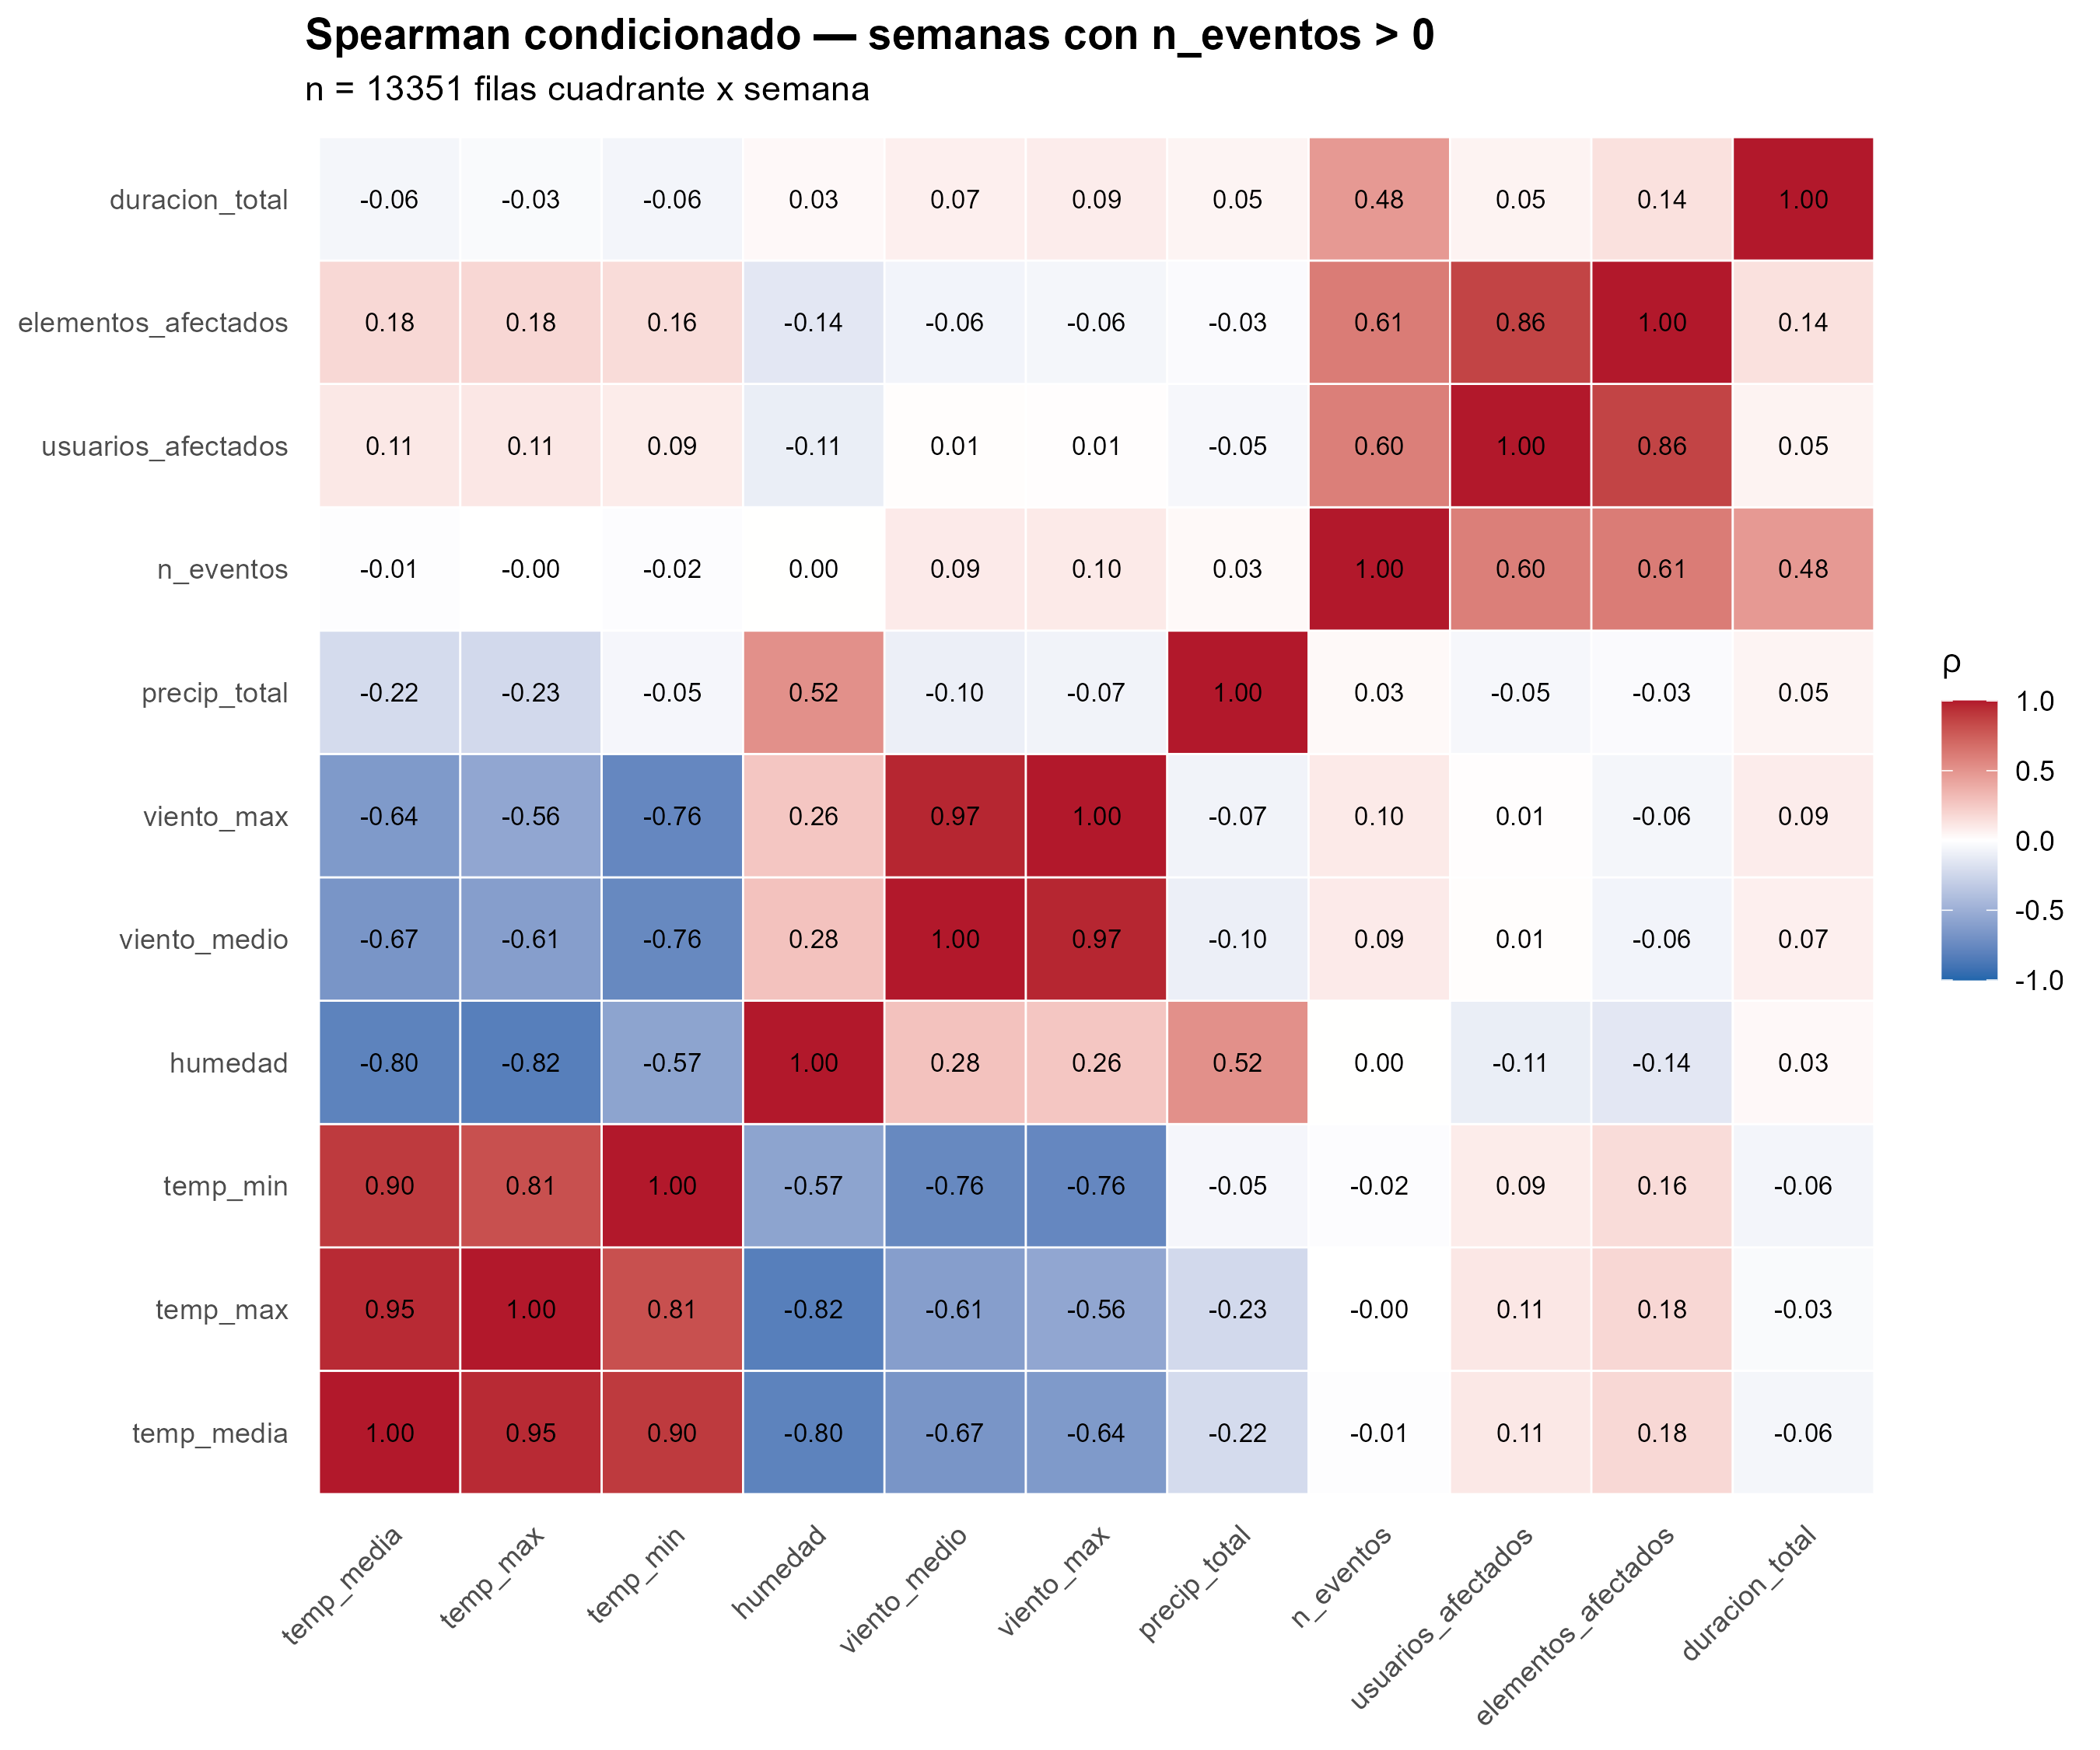
\includegraphics[width=0.92\textwidth]{img/heatmap_correlacion_condicionado_mod.png}
        \caption{Correlaciones de Spearman en semanas-cuadrante con \texttt{n\_eventos} $> 0$ ($n = 13\,351$).}
        \label{fig:heatmap_cor_condicionado}
    \end{figure}
    
    \noindent En síntesis, el análisis de correlación sobre $D_{\mathrm{mod}}$ confirma: (i)~\textit{alta redundancia} entre variables operativas de severidad y entre temperaturas/vientos del bloque climático; (ii)~una \textit{señal climática débil en términos bivariados}, encabezada por el viento ($\rho \approx 0{.}14$) y seguida por la precipitación ($\rho \approx 0{.}07$); y (iii)~\textit{asociaciones prácticamente nulas} de temperatura y humedad en el grano semanal. Estos hallazgos fundamentan conservar \texttt{viento\_medio\_semana} y \texttt{precip\_total\_semana} como candidatas climáticas, sujetas a la regla de disponibilidad \emph{ex ante} (rezago o pronóstico; Sección~\ref{sec:metodos-modelos}), la exclusión de variables climáticas redundantes y la fijación de la respuesta en \texttt{n\_eventos} y/o \texttt{duracion\_total}, dejando \texttt{usuarios\_afectados} y \texttt{elementos\_afectados} fuera del conjunto de predictoras contemporáneas (impacto posterior). Asimismo advierten que la Etapa~4 no debe apoyarse únicamente en covariables meteorológicas de la misma semana: la estructura temporal y territorial de la propia serie de eventos (Secciones~\ref{sec:analisis_temporal_eventos} y~\ref{sec:segmentacion_exploratoria}) concentra la mayor parte de la señal predictiva disponible. El análisis multivariado formal (VIF, redundancia simultánea) se desarrolla en la Sección~\ref{sec:evaluacion_multivariada}.
    
\subsection{Evaluación inicial de relaciones multivariadas}
\label{sec:evaluacion_multivariada}
    Con fundamento en las redundancias bivariadas identificadas en la Sección~\ref{sec:analisis_correlacion_asociacion}, se evaluaron las relaciones \textit{simultáneas} entre covariables sobre $D_{\mathrm{mod}}$ mediante VIF, PCA exploratorio, agrupamiento jerárquico de variables climáticas, correlación parcial y un GLM Poisson de diagnóstico (Sección~\ref{sec:metodos-modelos}). El procedimiento reproducible se documenta en el Apéndice~\ref{app:html-multivariado}.
    
    \paragraph{Multicolinealidad climática (VIF).} Se estimó un modelo auxiliar lineal \texttt{n\_eventos $\sim$} bloque climático completo para calcular el VIF de cada covariable. La Figura~\ref{fig:vif_clima_multivariado} muestra VIF elevados en \texttt{temp\_media\_semana} ($43{.}92$), \texttt{viento\_medio\_semana} ($24{.}22$), \texttt{viento\_max\_semana} ($22{.}58$), \texttt{temp\_max\_semana} ($17{.}27$) y \texttt{temp\_min\_semana} ($14{.}37$), mientras \texttt{precip\_total\_semana} ($1{.}50$) presenta inflación baja y \texttt{humedad\_media\_semana} ($5{.}68$) apenas moderada. Al restringir el bloque a \texttt{precip\_total\_semana}, \texttt{temp\_media\_semana}, \texttt{humedad\_media\_semana} y \texttt{viento\_medio\_semana}, los VIF descienden a valores aceptables (máximo $7{.}21$ en temperatura media; Tabla~\ref{tab:vif_reducido}).
    
    \begin{figure}[!htbp]
        \centering
        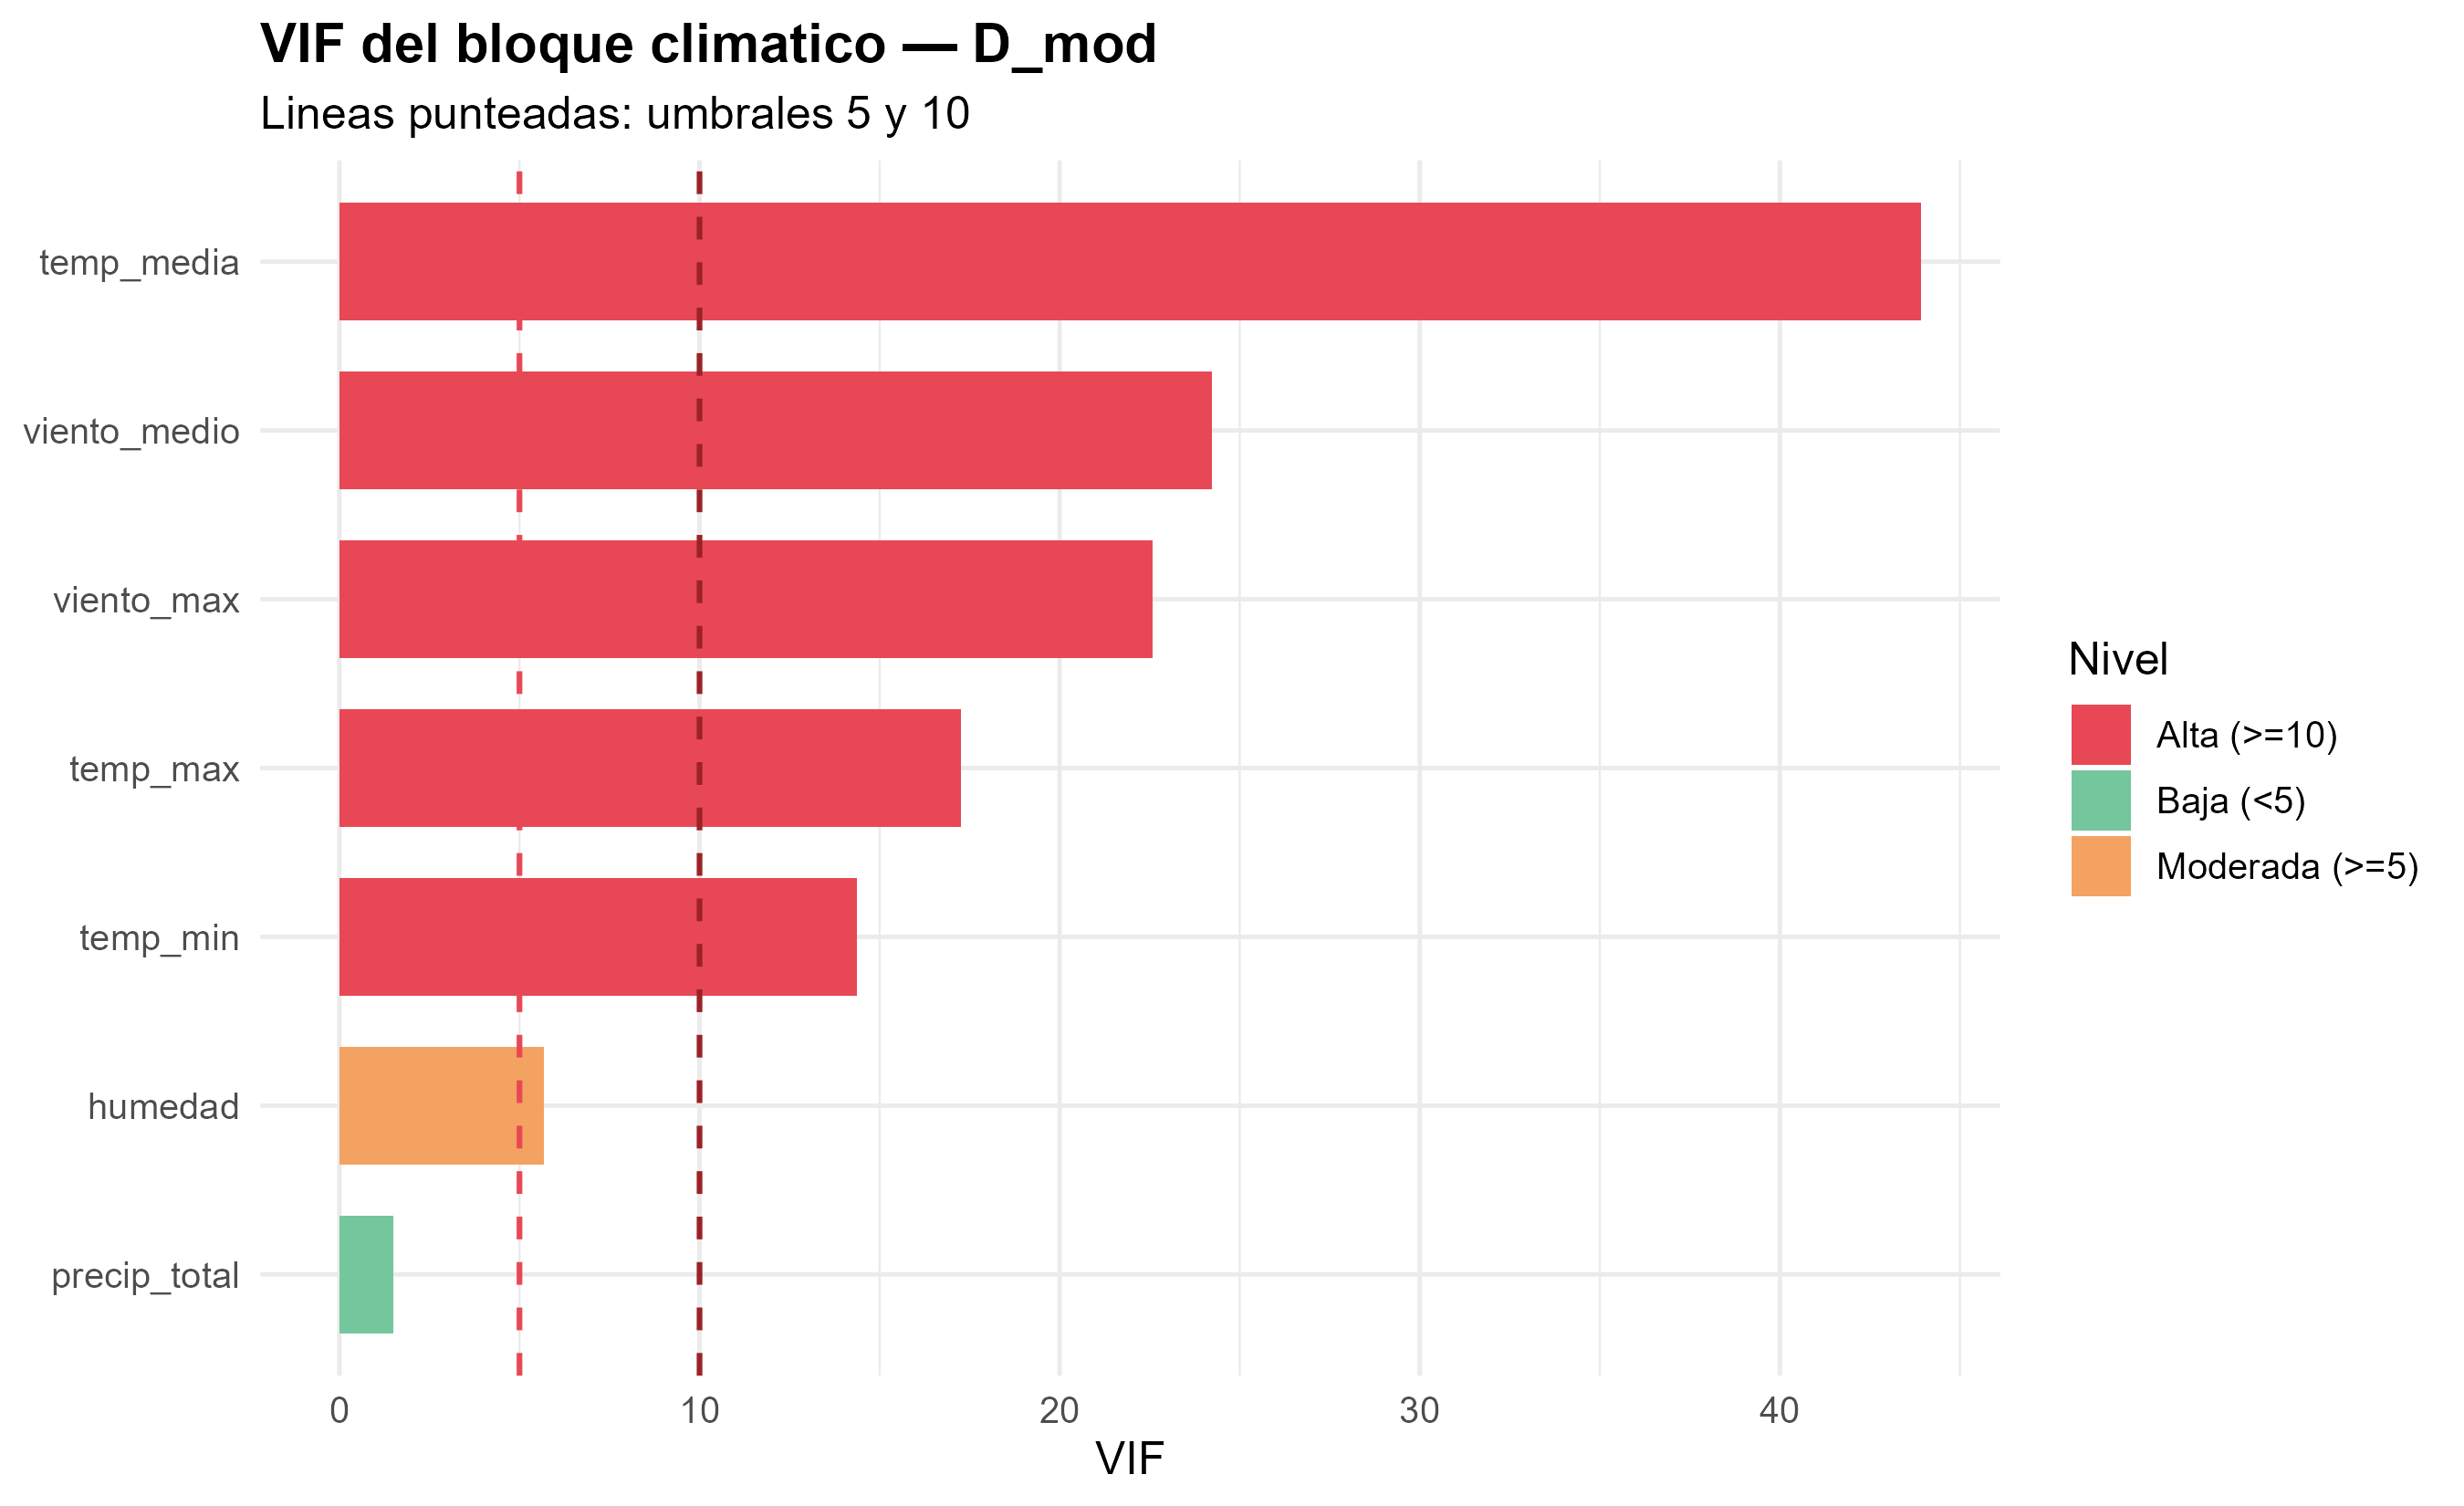
\includegraphics[width=0.92\textwidth]{img/vif_clima_multivariado_mod.png}
        \caption{Inflación de varianza en el bloque climático (modelo auxiliar \texttt{n\_eventos $\sim$ clima}; $D_{\mathrm{mod}}$).}
        \label{fig:vif_clima_multivariado}
    \end{figure}
    
    \begin{table}[!htbp]
    \centering
    \small
    \caption{Inflación de varianza con subconjunto climático reducido propuesto para la Etapa~4}
    \label{tab:vif_reducido}
    \begin{tabular}{@{}l r@{}}
    \toprule
    \textbf{Variable} & \textbf{VIF} \\
    \midrule
    \texttt{temp\_media\_semana}     & 7.21 \\
    \texttt{humedad\_media\_semana}  & 4.47 \\
    \texttt{viento\_medio\_semana}   & 3.27 \\
    \texttt{precip\_total\_semana}   & 1.49 \\
    \bottomrule
    \end{tabular}
    \end{table}
    
    Se realizó adicionalmente un PCA exploratorio del bloque climático como diagnóstico de redundancia (no como fuente de predictoras finales); no se emplea como paso obligatorio del modelado. El detalle completo (variables de entrada, condiciones de aplicación, varianza retenida y cargas) se documenta en el Apéndice~\ref{app:pca-exploratorio}.
    
    \paragraph{Agrupamiento jerárquico.} El dendrograma de la Figura~\ref{fig:dendrograma_clima} confirma dos clusters principales: (i)~temperaturas y vientos, altamente intercorrelados; y (ii)~\texttt{precip\_total\_semana}, relativamente aislada. Este resultado valida la exclusión de \texttt{temp\_max\_semana}, \texttt{temp\_min\_semana} y \texttt{viento\_max\_semana} del conjunto predictor reducido.
    
    \begin{figure}[!htbp]
        \centering
        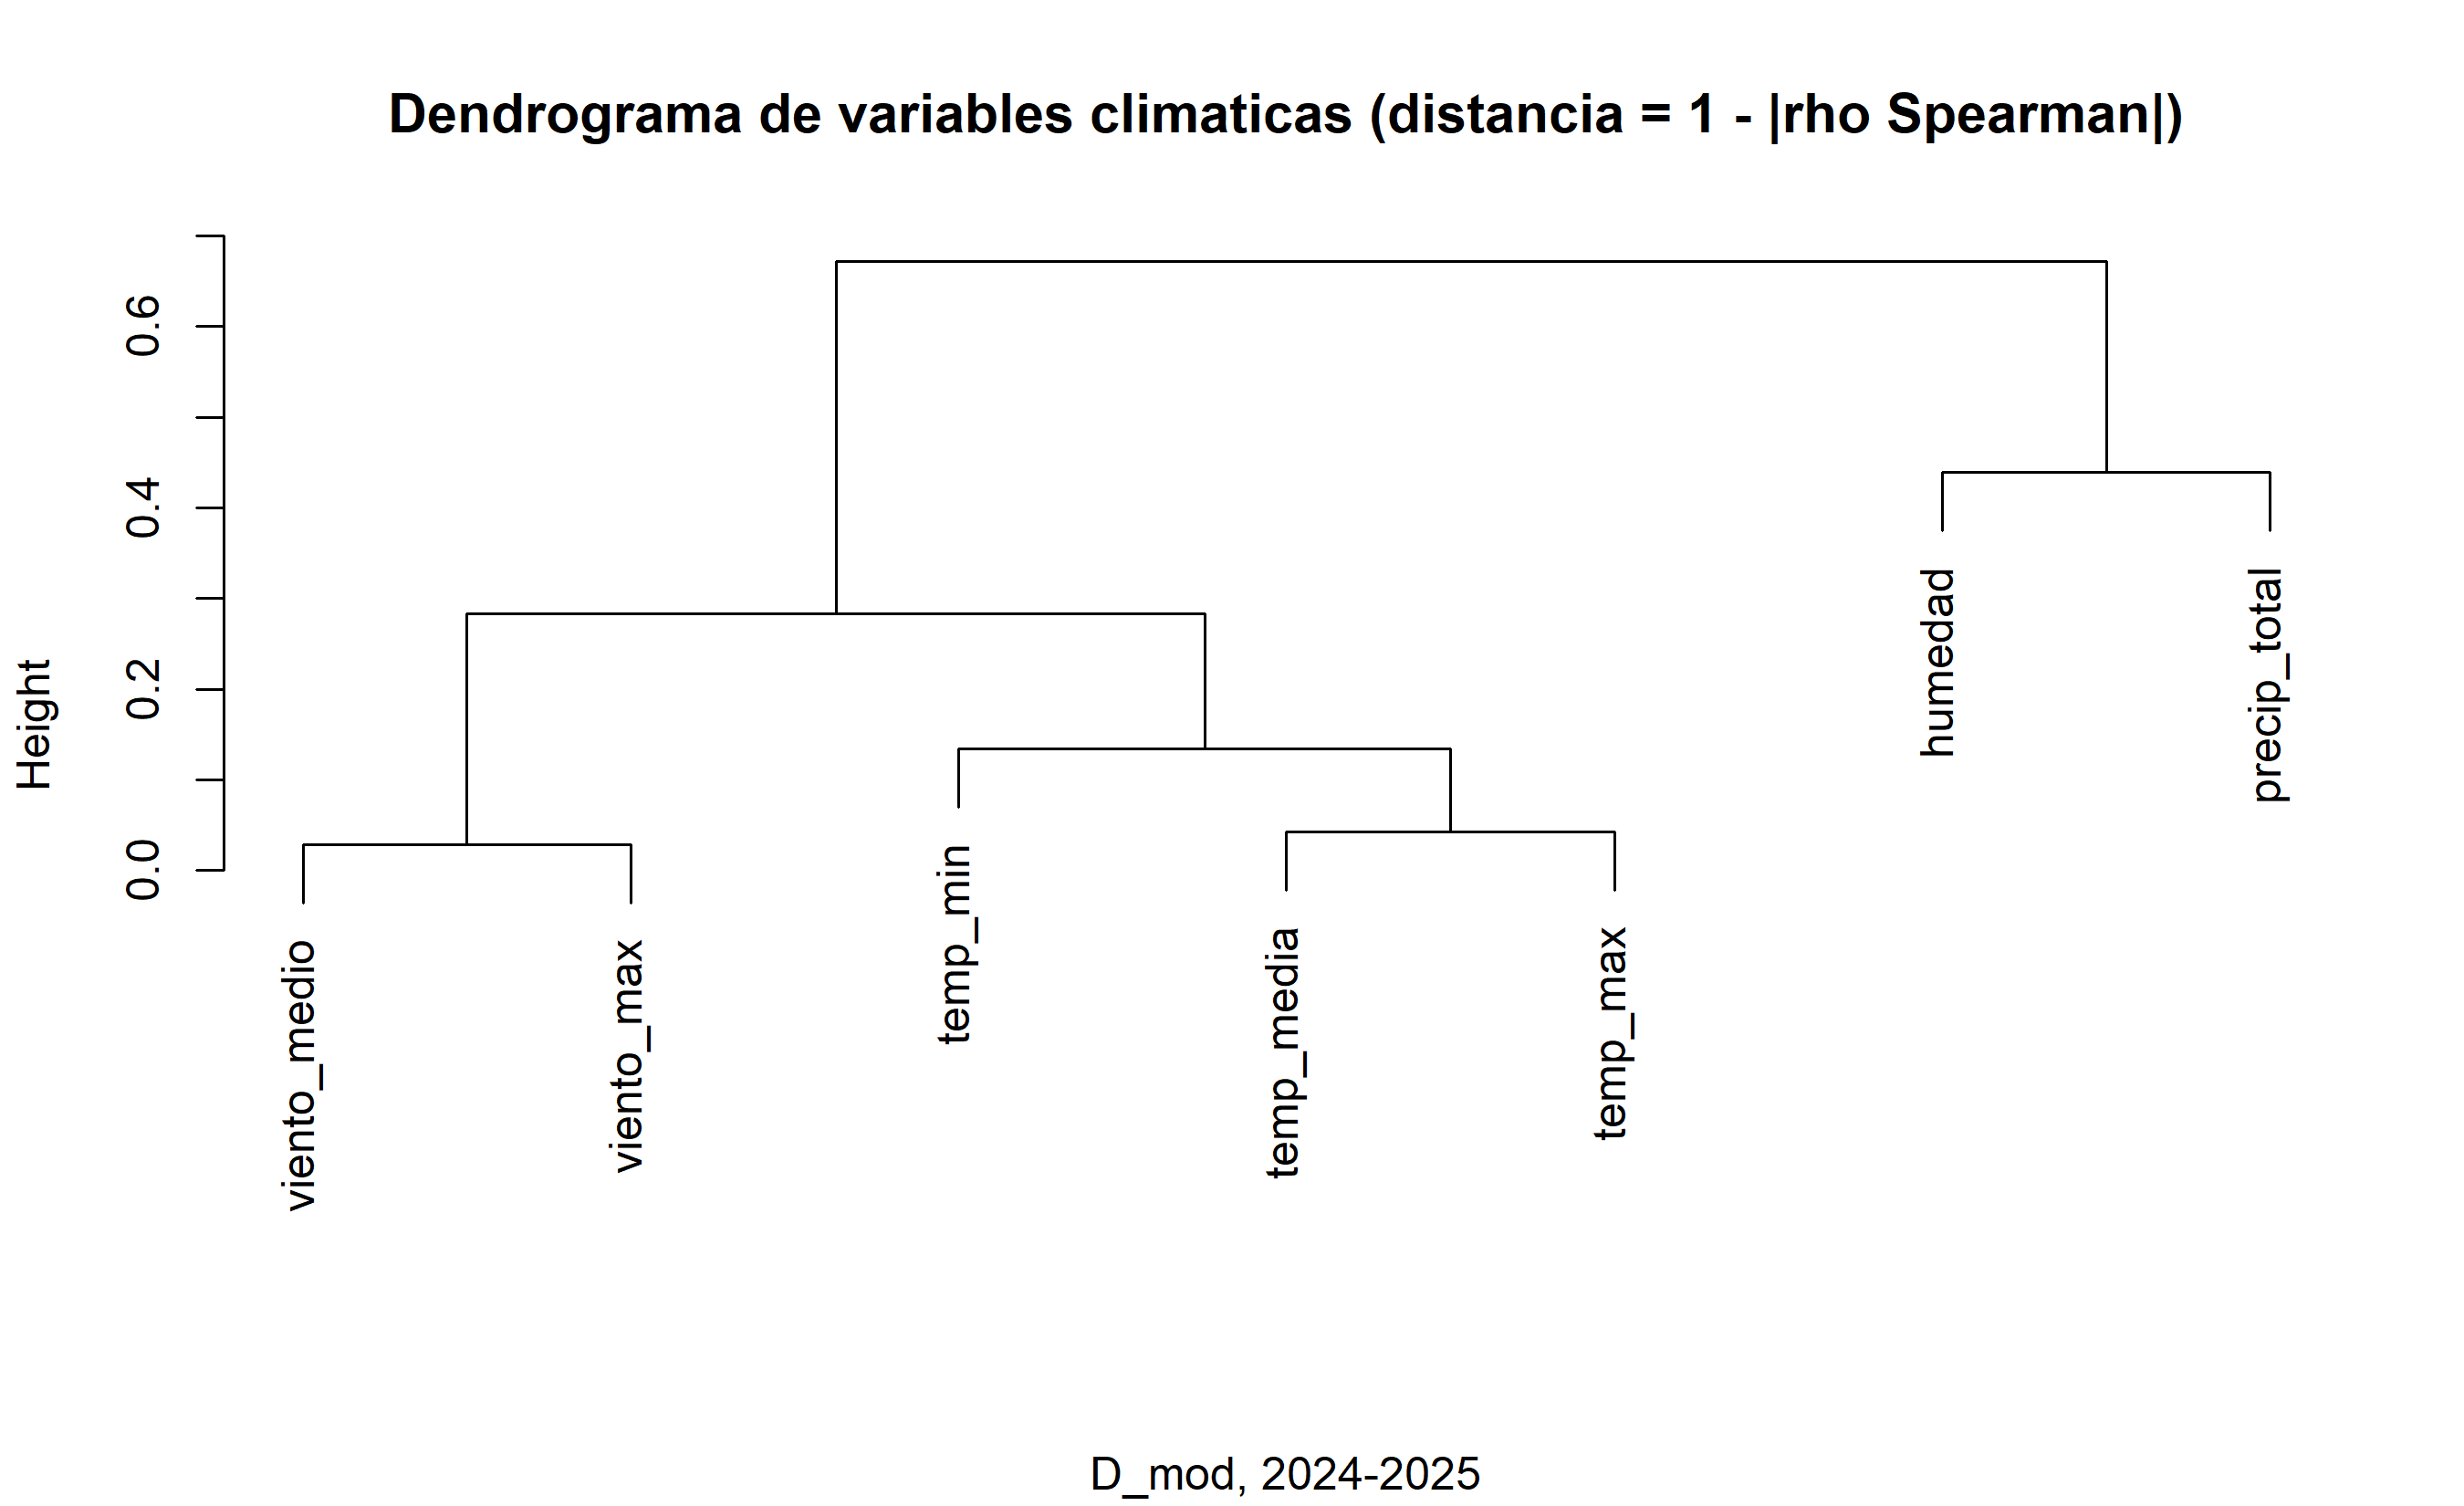
\includegraphics[width=0.95\textwidth]{img/dendrograma_clima_multivariado_mod.png}
        \caption{Agrupamiento de redundancias entre variables climáticas (Sección~\ref{sec:metodos-modelos}).}
        \label{fig:dendrograma_clima}
    \end{figure}
    
    \paragraph{Asociación multivariada clima $\rightarrow$ \texttt{n\_eventos}.} La correlación parcial de Spearman entre precipitación y \texttt{n\_eventos}, controlando \texttt{temp\_media\_semana} y \texttt{viento\_medio\_semana}, es $\rho = 0{.}114$, casi el doble del valor bivariado ($\rho = 0{.}065$). El aumento al condicionar indica que temperatura y viento, correlacionadas con la precipitación, enmascaraban parcialmente su asociación con los eventos; aun así, la magnitud sigue siendo modesta. Un GLM Poisson exploratorio con el subconjunto reducido (Figura~\ref{fig:glm_coef_multivariado}) arroja coeficientes positivos y significativos para las cuatro covariables, con la temperatura media estandarizada ($\hat{\beta} = 0{.}81$) y el viento medio estandarizado ($\hat{\beta} = 0{.}73$) como efectos dominantes, seguidos de la humedad ($\hat{\beta} = 0{.}35$) y de la precipitación en transformación logarítmica desplazada ($\hat{\beta} = 0{.}13$; todos con $p < 0{.}001$). Este contraste con el orden bivariado, donde las temperaturas eran irrelevantes, es consistente con la multicolinealidad diagnosticada por el VIF y refuerza que los coeficientes del bloque climático completo no admiten lectura causal individual; se reportan como diagnóstico exploratorio.
    
    \begin{figure}[!htbp]
        \centering
        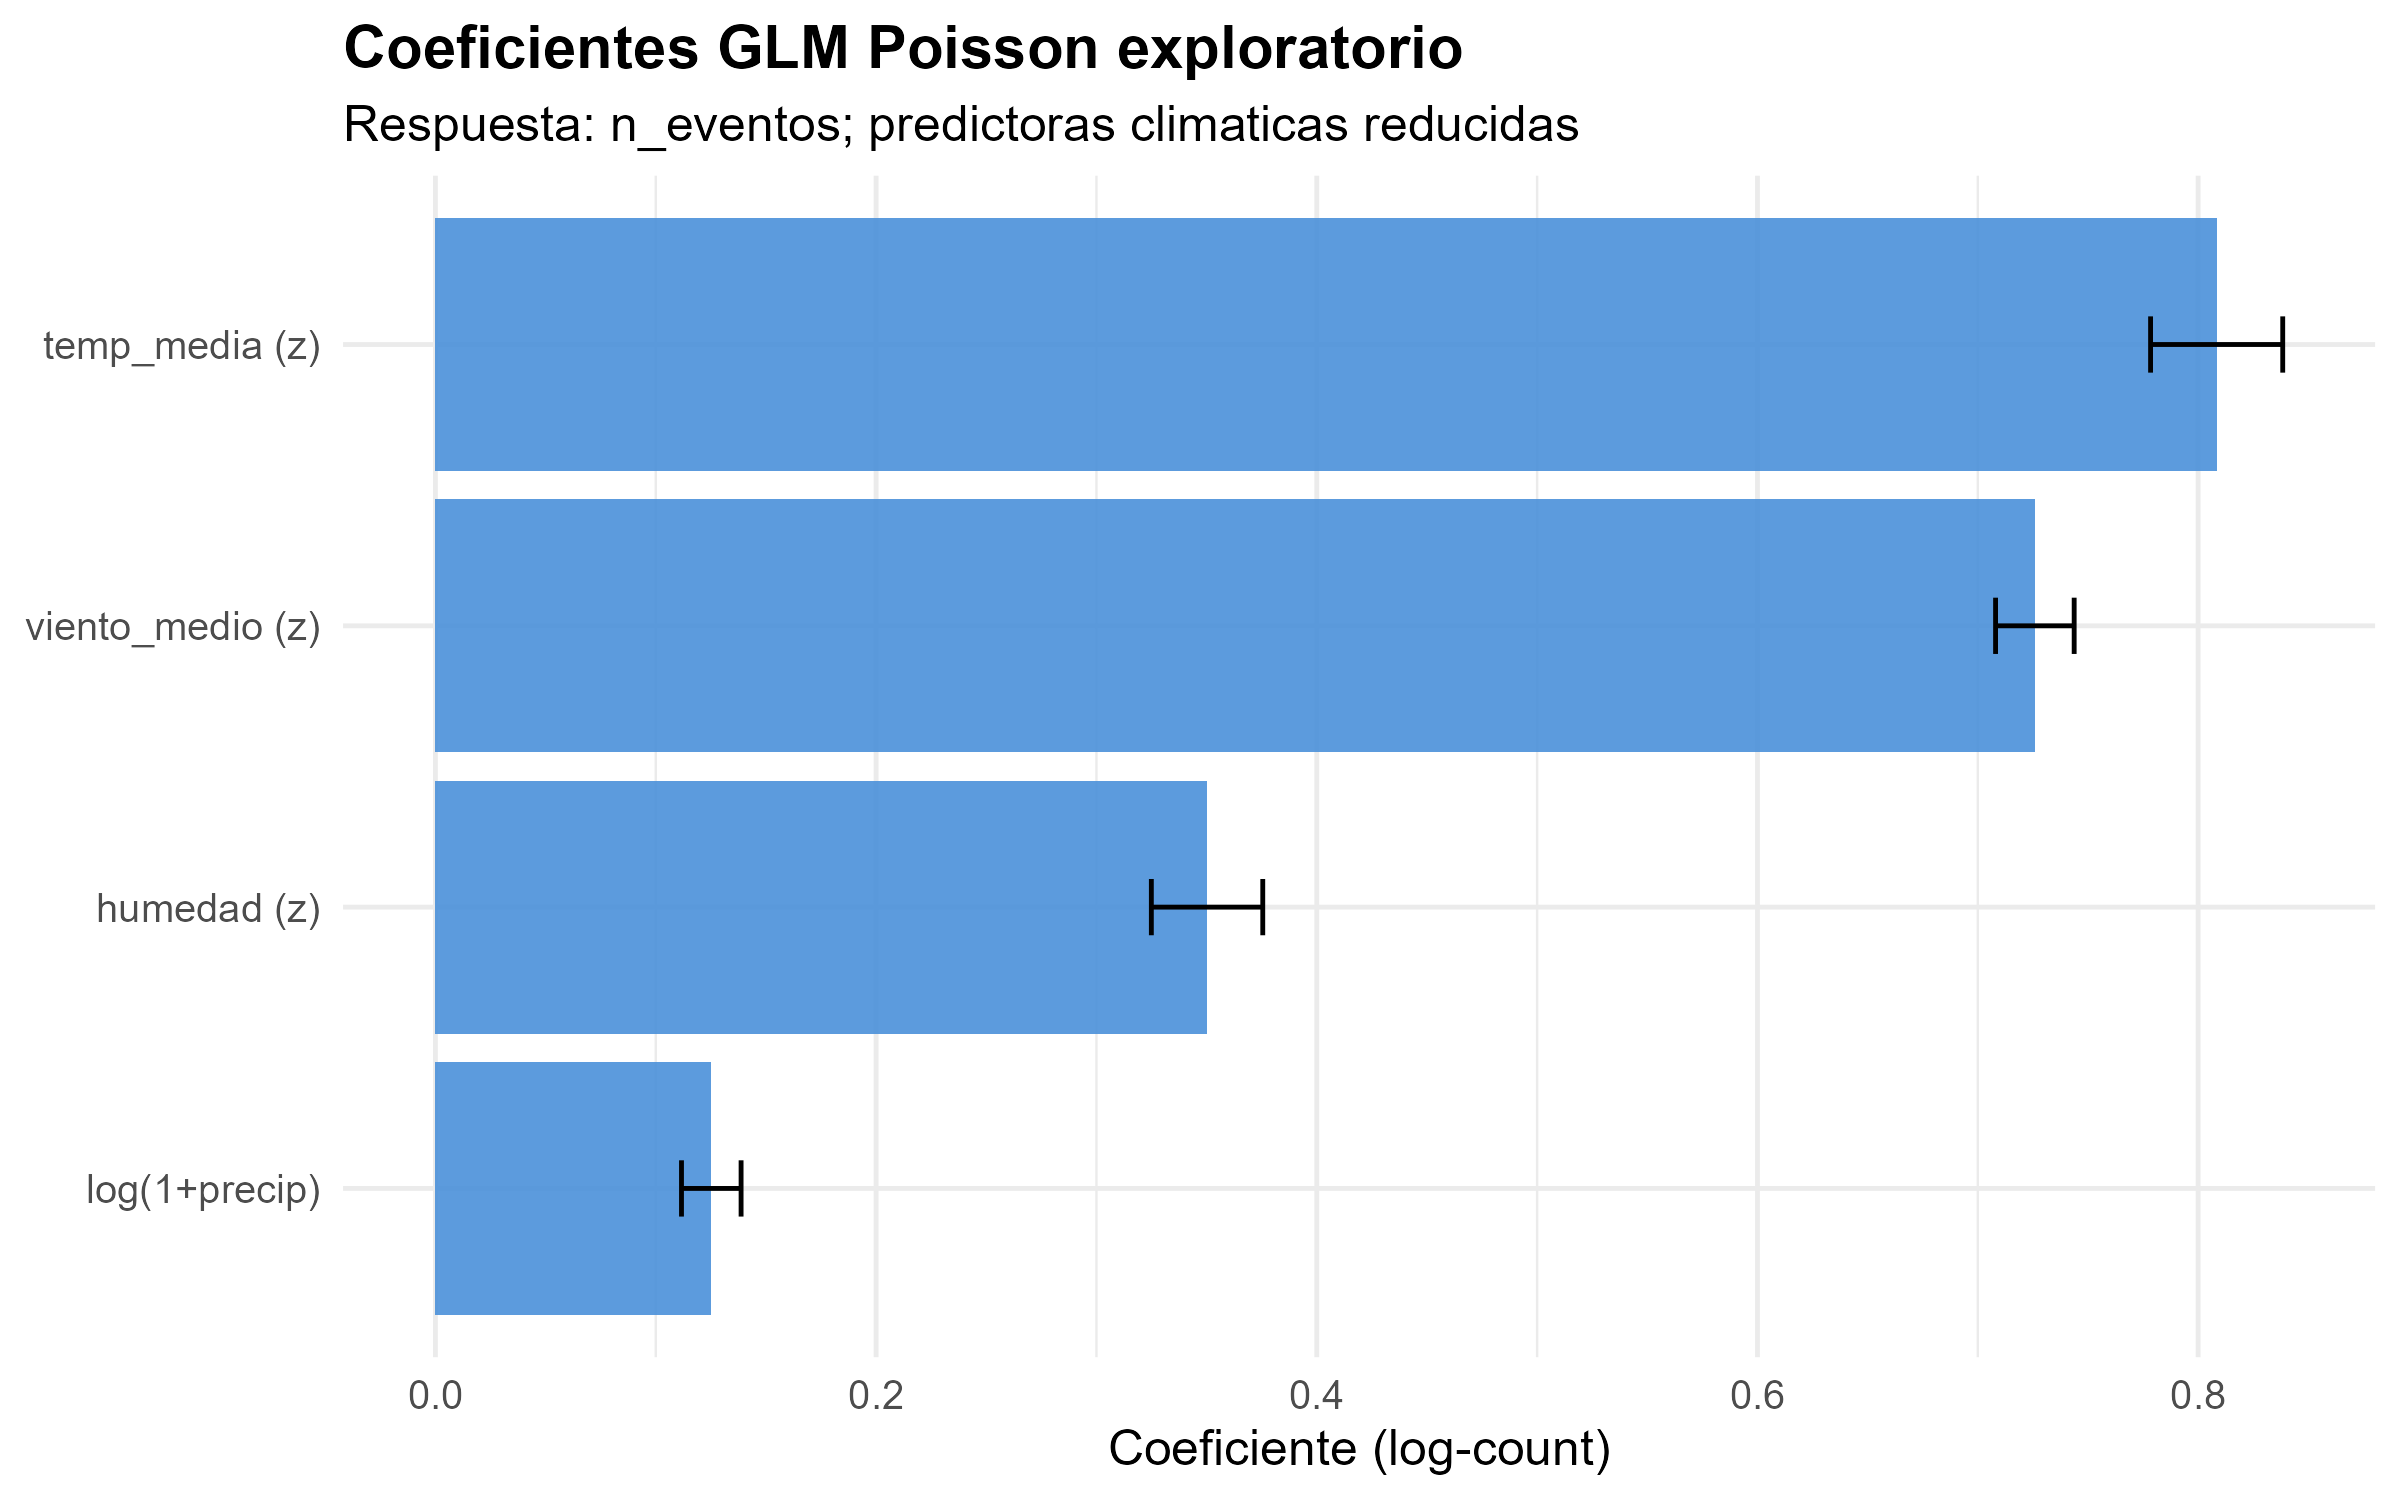
\includegraphics[width=0.82\textwidth]{img/glm_coef_clima_multivariado_mod.png}
        \caption{Efecto conjunto del clima reducido sobre la frecuencia de eventos (diagnóstico EDA).}
        \label{fig:glm_coef_multivariado}
    \end{figure}
    
    De forma análoga se aplicó un PCA exploratorio al bloque operativo (frecuencia, afectación y duración) para delimitar dimensiones de impacto, sin emplearlo como fuente de predictoras. El detalle completo se documenta en el Apéndice~\ref{app:pca-exploratorio}.
    
    \noindent En síntesis, la evaluación multivariada sobre $D_{\mathrm{mod}}$ recomienda: (i)~predictoras climáticas \texttt{precip\_total\_semana}, \texttt{temp\_media\_semana}, \texttt{humedad\_media\_semana} y \texttt{viento\_medio\_semana}, justificadas por loadings, VIF y dendrograma (el PCA no se usa como modelo predictivo, sino como diagnóstico de redundancia); (ii)~$SAIFI$ y $SAIDI$ como variables respuesta del modelado, construidas en la Etapa~4; (iii)~exclusión de temperaturas extremas y viento máximo por redundancia simultánea; (iv)~expectativas moderadas sobre la capacidad explicativa del bloque meteorológico contemporáneo, dado el tamaño reducido de las asociaciones observadas, lo que hace aconsejable complementarlo con rezagos de la propia serie de eventos y con la estratificación territorial; y (v)~uso de \texttt{usuarios\_afectados} solo en el numerador de $Y$, no como predictora contemporánea. Estos criterios se operacionalizan en la depuración cuantitativa y la construcción de matrices de diseño de la Etapa~4.
    
\subsection{Segmentación exploratoria}
\label{sec:segmentacion_exploratoria}
    Con fundamento en la segmentación territorial introducida en la Sección~\ref{sec:identificacion_patrones_tendencias}, se profundizó la heterogeneidad de $D_{\mathrm{mod}}$ mediante perfiles comparativos por nivel de actividad, evolución 2024--2025, estratificación por régimen de precipitación semanal y clustering multivariado de cuadrantes. El procedimiento reproducible se documenta en el Apéndice~\ref{app:html-segmentacion}.
    
    \paragraph{Perfiles por nivel de actividad.} Sobre los $344$ cuadrantes del periodo, la clasificación Baja/Media/Alta (cuantiles P50 y P85 entre cuadrantes con eventos) arroja: $162$ cuadrantes baja ($47{.}1$~\%), $113$ media ($32{.}8$~\%) y $49$ alta ($14{.}2$~\%); $20$ cuadrantes ($5{.}8$~\%) no registraron eventos. Los perfiles acumulados, resumidos en la Figura~\ref{fig:heatmap_perfiles_segmentacion}, muestran escalamiento marcado en las variables operativas: media de $22$ eventos por cuadrante en nivel baja frente a $114{.}6$ en media y $344{.}7$ en alta, con usuarios afectados medios de $1\,588$ a $88\,534$. El clima, en cambio, no acompaña ese escalamiento: la precipitación semanal media desciende ligeramente de $19{.}6$~mm (baja) a $18{.}5$~mm (media) y $17{.}0$~mm (alta), de modo que los estratos de mayor actividad no son los más lluviosos. La Figura~\ref{fig:boxplot_nivel_segmentacion} confirma que la dispersión semanal de \texttt{n\_eventos} crece con el estrato territorial.
    
    
    \begin{figure}[!htbp]
        \centering
        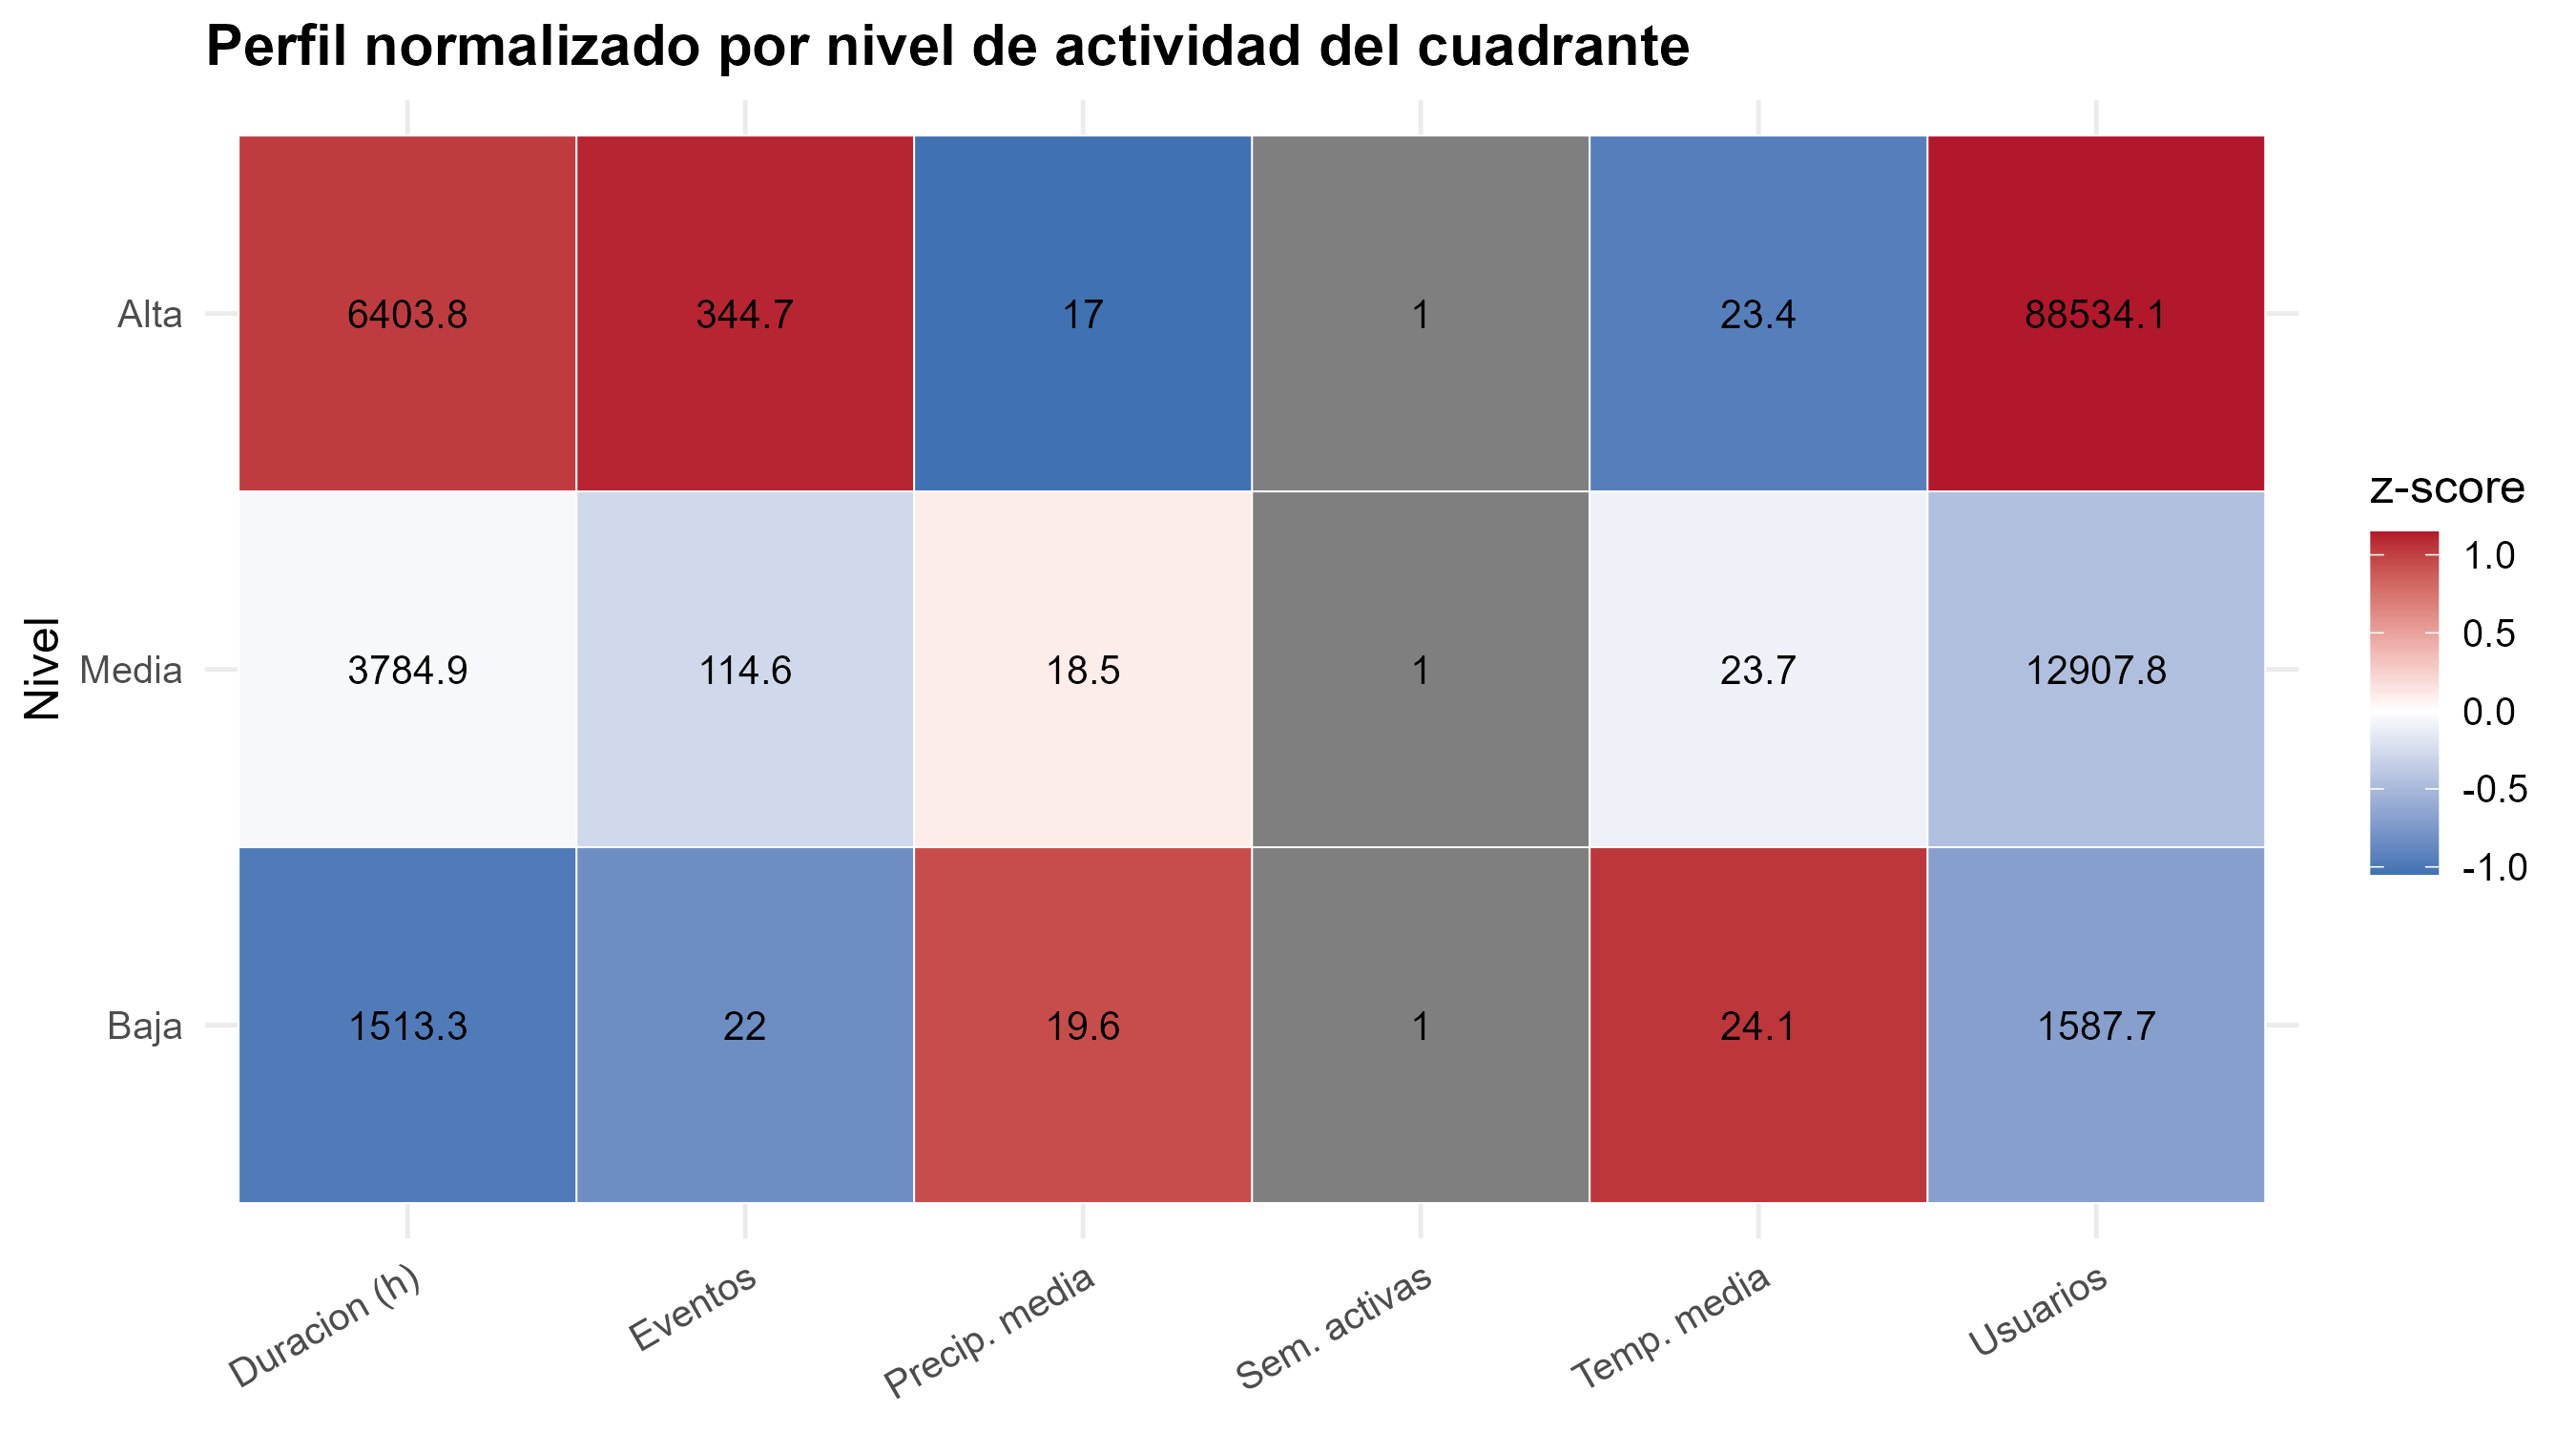
\includegraphics[width=0.88\textwidth]{img/heatmap_perfiles_nivel_segmentacion_mod.png}
        \caption{Perfil normalizado por nivel de actividad (eventos, usuarios, duración, semanas activas, clima).}
        \label{fig:heatmap_perfiles_segmentacion}
    \end{figure}
    
    \paragraph{Evolución 2024 vs 2025 por estrato.} El total territorial ascendió de $15\,211$ eventos en 2024 ($287$/semana) a $18\,199$ en 2025 ($350$/semana). Al desagregar por nivel fijado en el periodo completo, el ratio medio 2025/2024 es homogéneo: $1{.}24$ (baja), $1{.}26$ (media) y $1{.}24$ (alta), lo que indica incremento transversal sin reordenamiento fuerte de la jerarquía territorial (Figura~\ref{fig:barras_anio_nivel_segmentacion}). El crecimiento observado en 2024--2025 debe interpretarse en coherencia con la homogeneización de codificación activo/sitio bajo OMS-SP7 (Sección~\ref{sec:delimitacion_temporal_modelado}), no exclusivamente como deterioro operativo.
    
    \begin{figure}[!htbp]
        \centering
        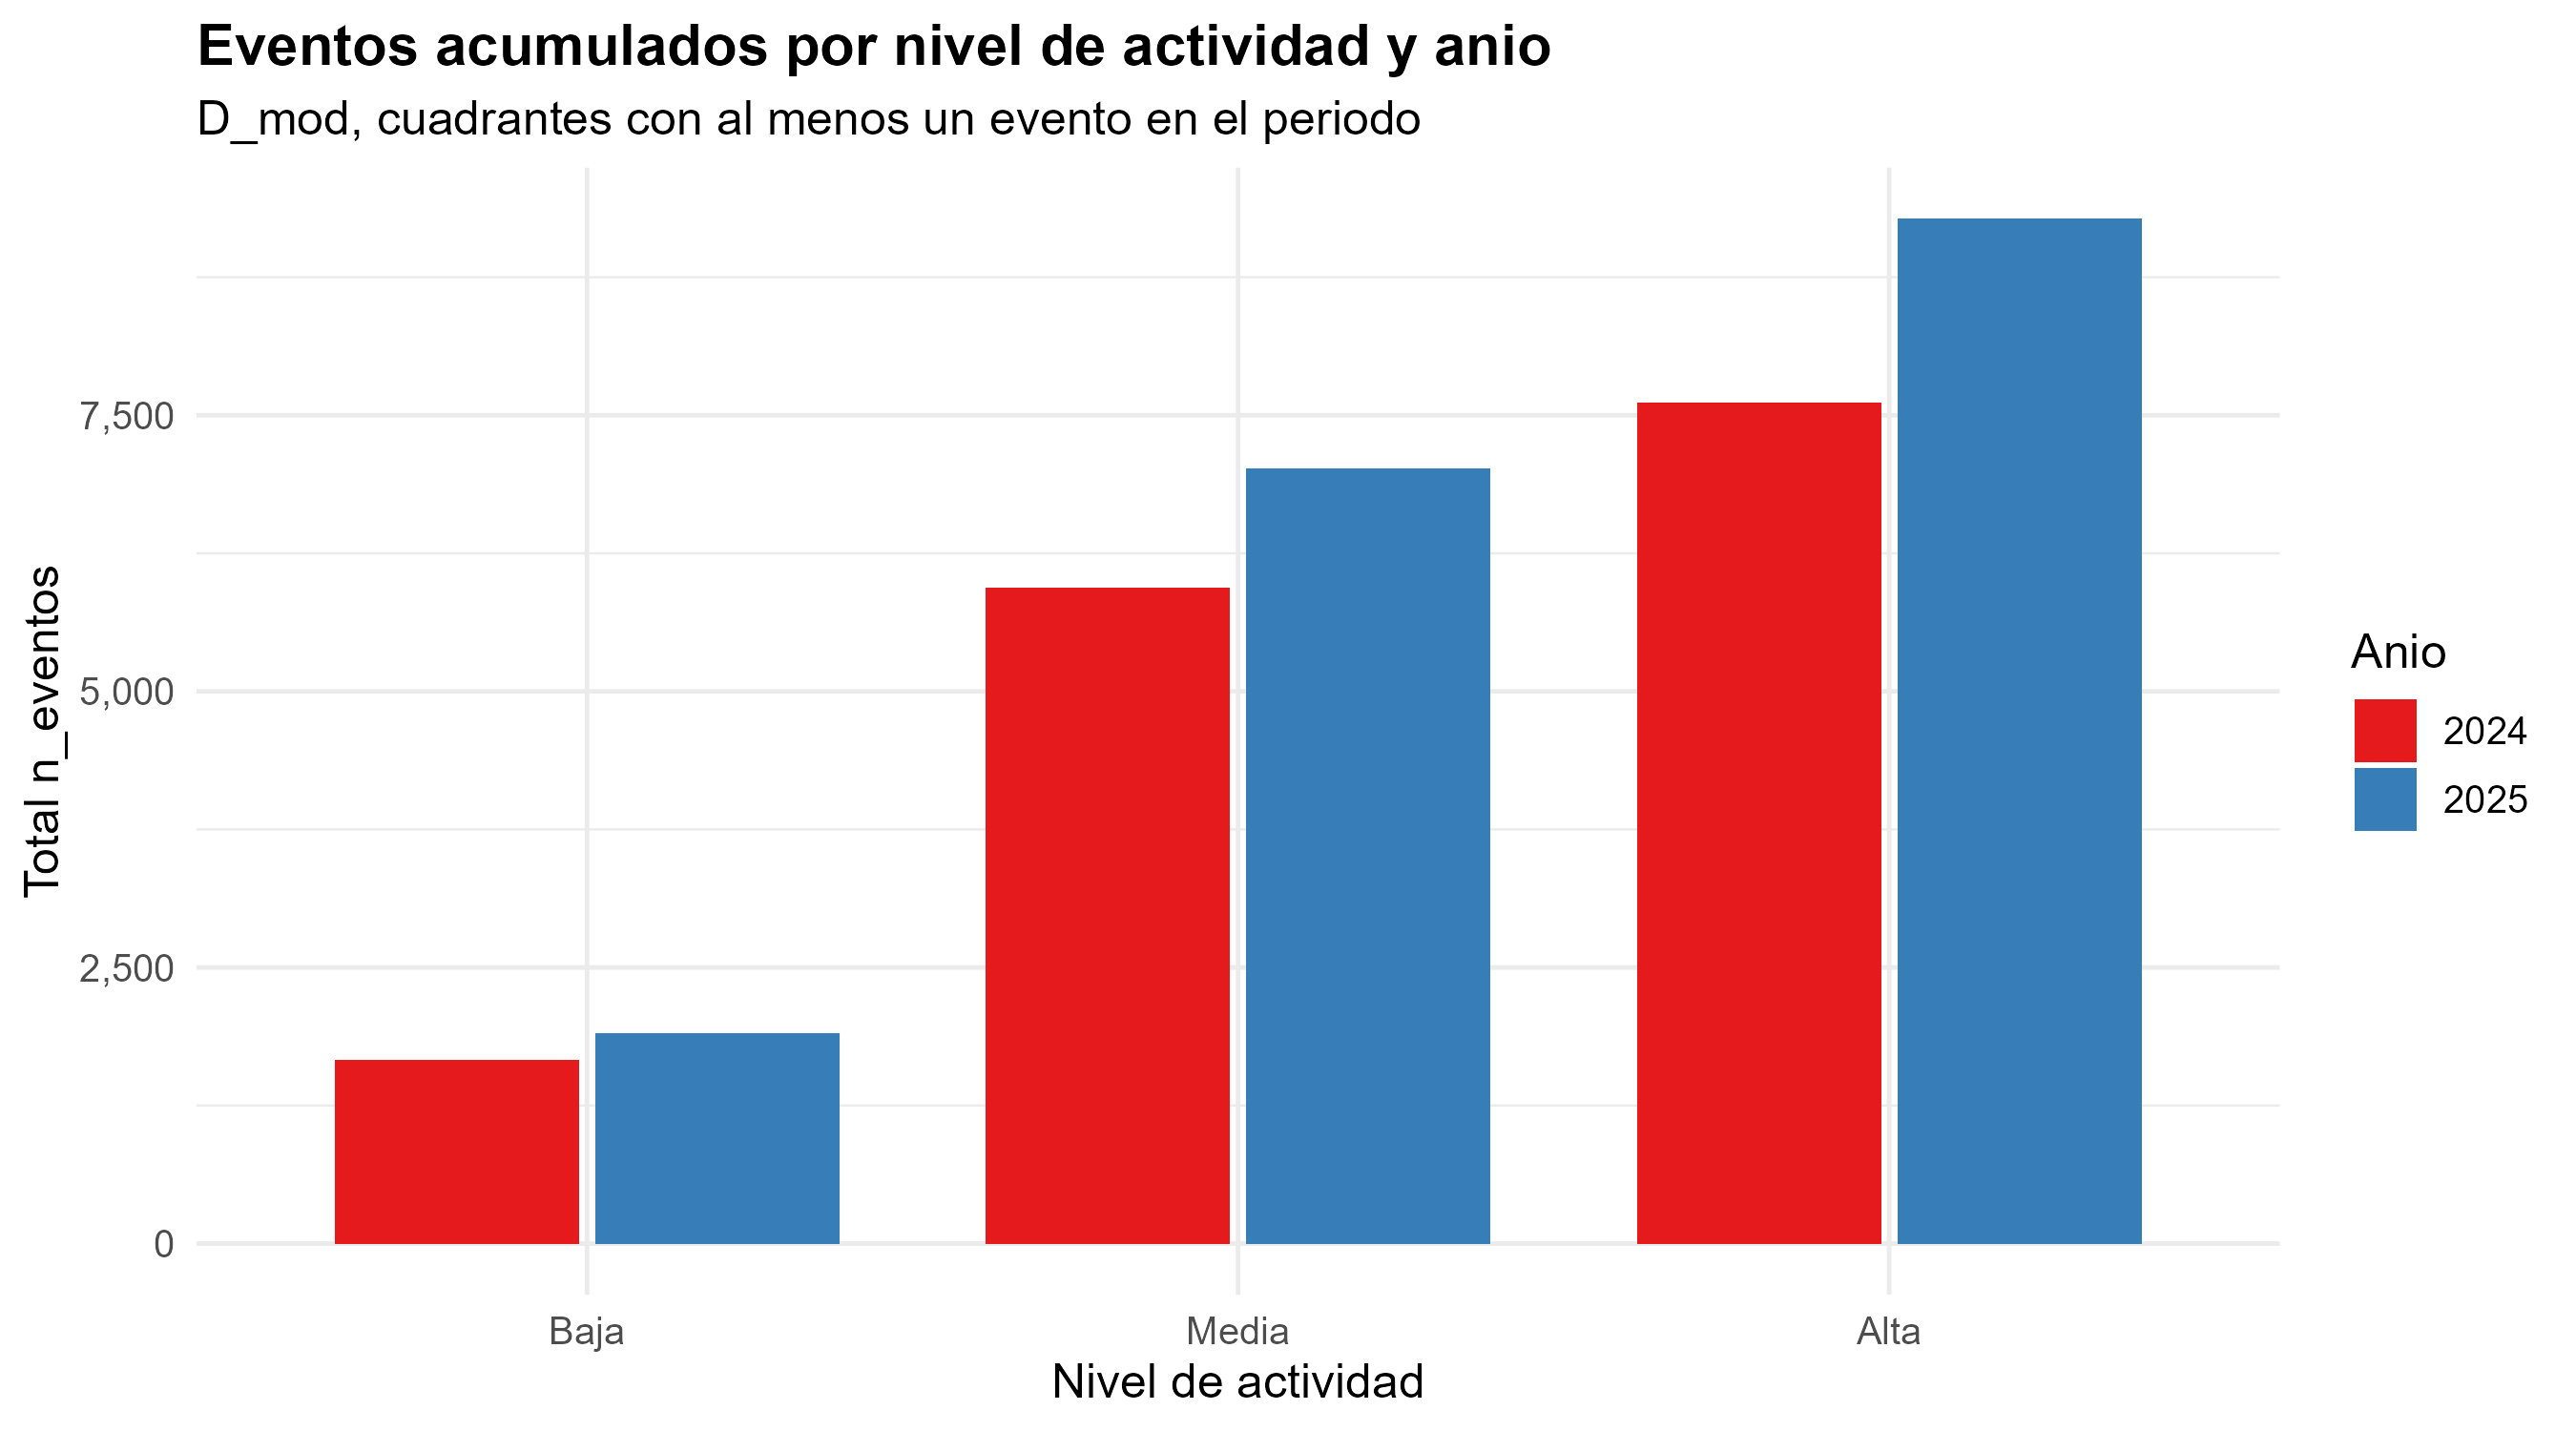
\includegraphics[width=0.85\textwidth]{img/barras_eventos_anio_nivel_segmentacion_mod.png}
        \caption{Eventos acumulados por nivel de actividad y año en $D_{\mathrm{mod}}$.}
        \label{fig:barras_anio_nivel_segmentacion}
    \end{figure}
    
    \paragraph{Régimen climático semanal.} Se estratificaron las filas según el percentil~$75$ de \texttt{precip\_total\_semana} ($24{.}7$~mm). Las semanas lluviosas ($25$~\% de las filas; $9\,030$ observaciones) presentan media de \texttt{n\_eventos} de $0{.}918$, prácticamente igual a la de las semanas secas ($0{.}927$; $75$~\%; $27\,090$ filas), con $37{.}7$~\% frente a $36{.}7$~\% de semanas con al menos un evento. La prueba de Wilcoxon no detecta diferencia significativa ($p = 0{.}175$; Figura~\ref{fig:boxplot_regimen_segmentacion}), resultado consistente con la débil asociación bivariada precipitación--eventos de la Sección~\ref{sec:analisis_correlacion_asociacion}. La dicotomización por umbral resulta así insuficiente para separar regímenes operativos: si la lluvia tiene efecto, opera a través de la intensidad de episodios puntuales y no del acumulado semanal, lo que sugiere explorar en la Etapa~4 indicadores de intensidad diaria o de número de días de lluvia dentro de la semana.
    
    
    \paragraph{Clustering multivariado de cuadrantes.} Se aplicó k-means ($k = 4$) sobre cuadrantes con al menos un evento, con variables estandarizadas de frecuencia, severidad, duración, clima y altitud (Sección~\ref{sec:metodos-modelos}; excluyendo covariables de varianza nula). El mapa de la Figura~\ref{fig:mapa_cluster_segmentacion} y el heatmap de la Figura~\ref{fig:heatmap_cluster_segmentacion} distinguen: C3 ($1$ cuadrante; $2\,224$ eventos; hub extremo), C1 ($139$ cuadrantes; media $107{.}4$ eventos; mayor severidad y duración acumulada, altitud media $496$~m), C4 ($126$ cuadrantes; media $97{.}7$ eventos; el estrato de mayor altitud, $1\,741$~m) y C2 ($58$ cuadrantes; media $68{.}0$ eventos; el más lluvioso, $26{.}2$~mm semanales, y el de menor duración acumulada). Que el cluster más lluvioso sea también el de menor actividad refuerza que la precipitación no ordena por sí sola el territorio; la altitud y el perfil de severidad discriminan más. La existencia de un hub aislado y de estratos con perfiles distinguibles respalda evaluar modelado global frente a estratificación por cluster en la Etapa~4.
    
    \begin{figure}[!htbp]
        \centering
        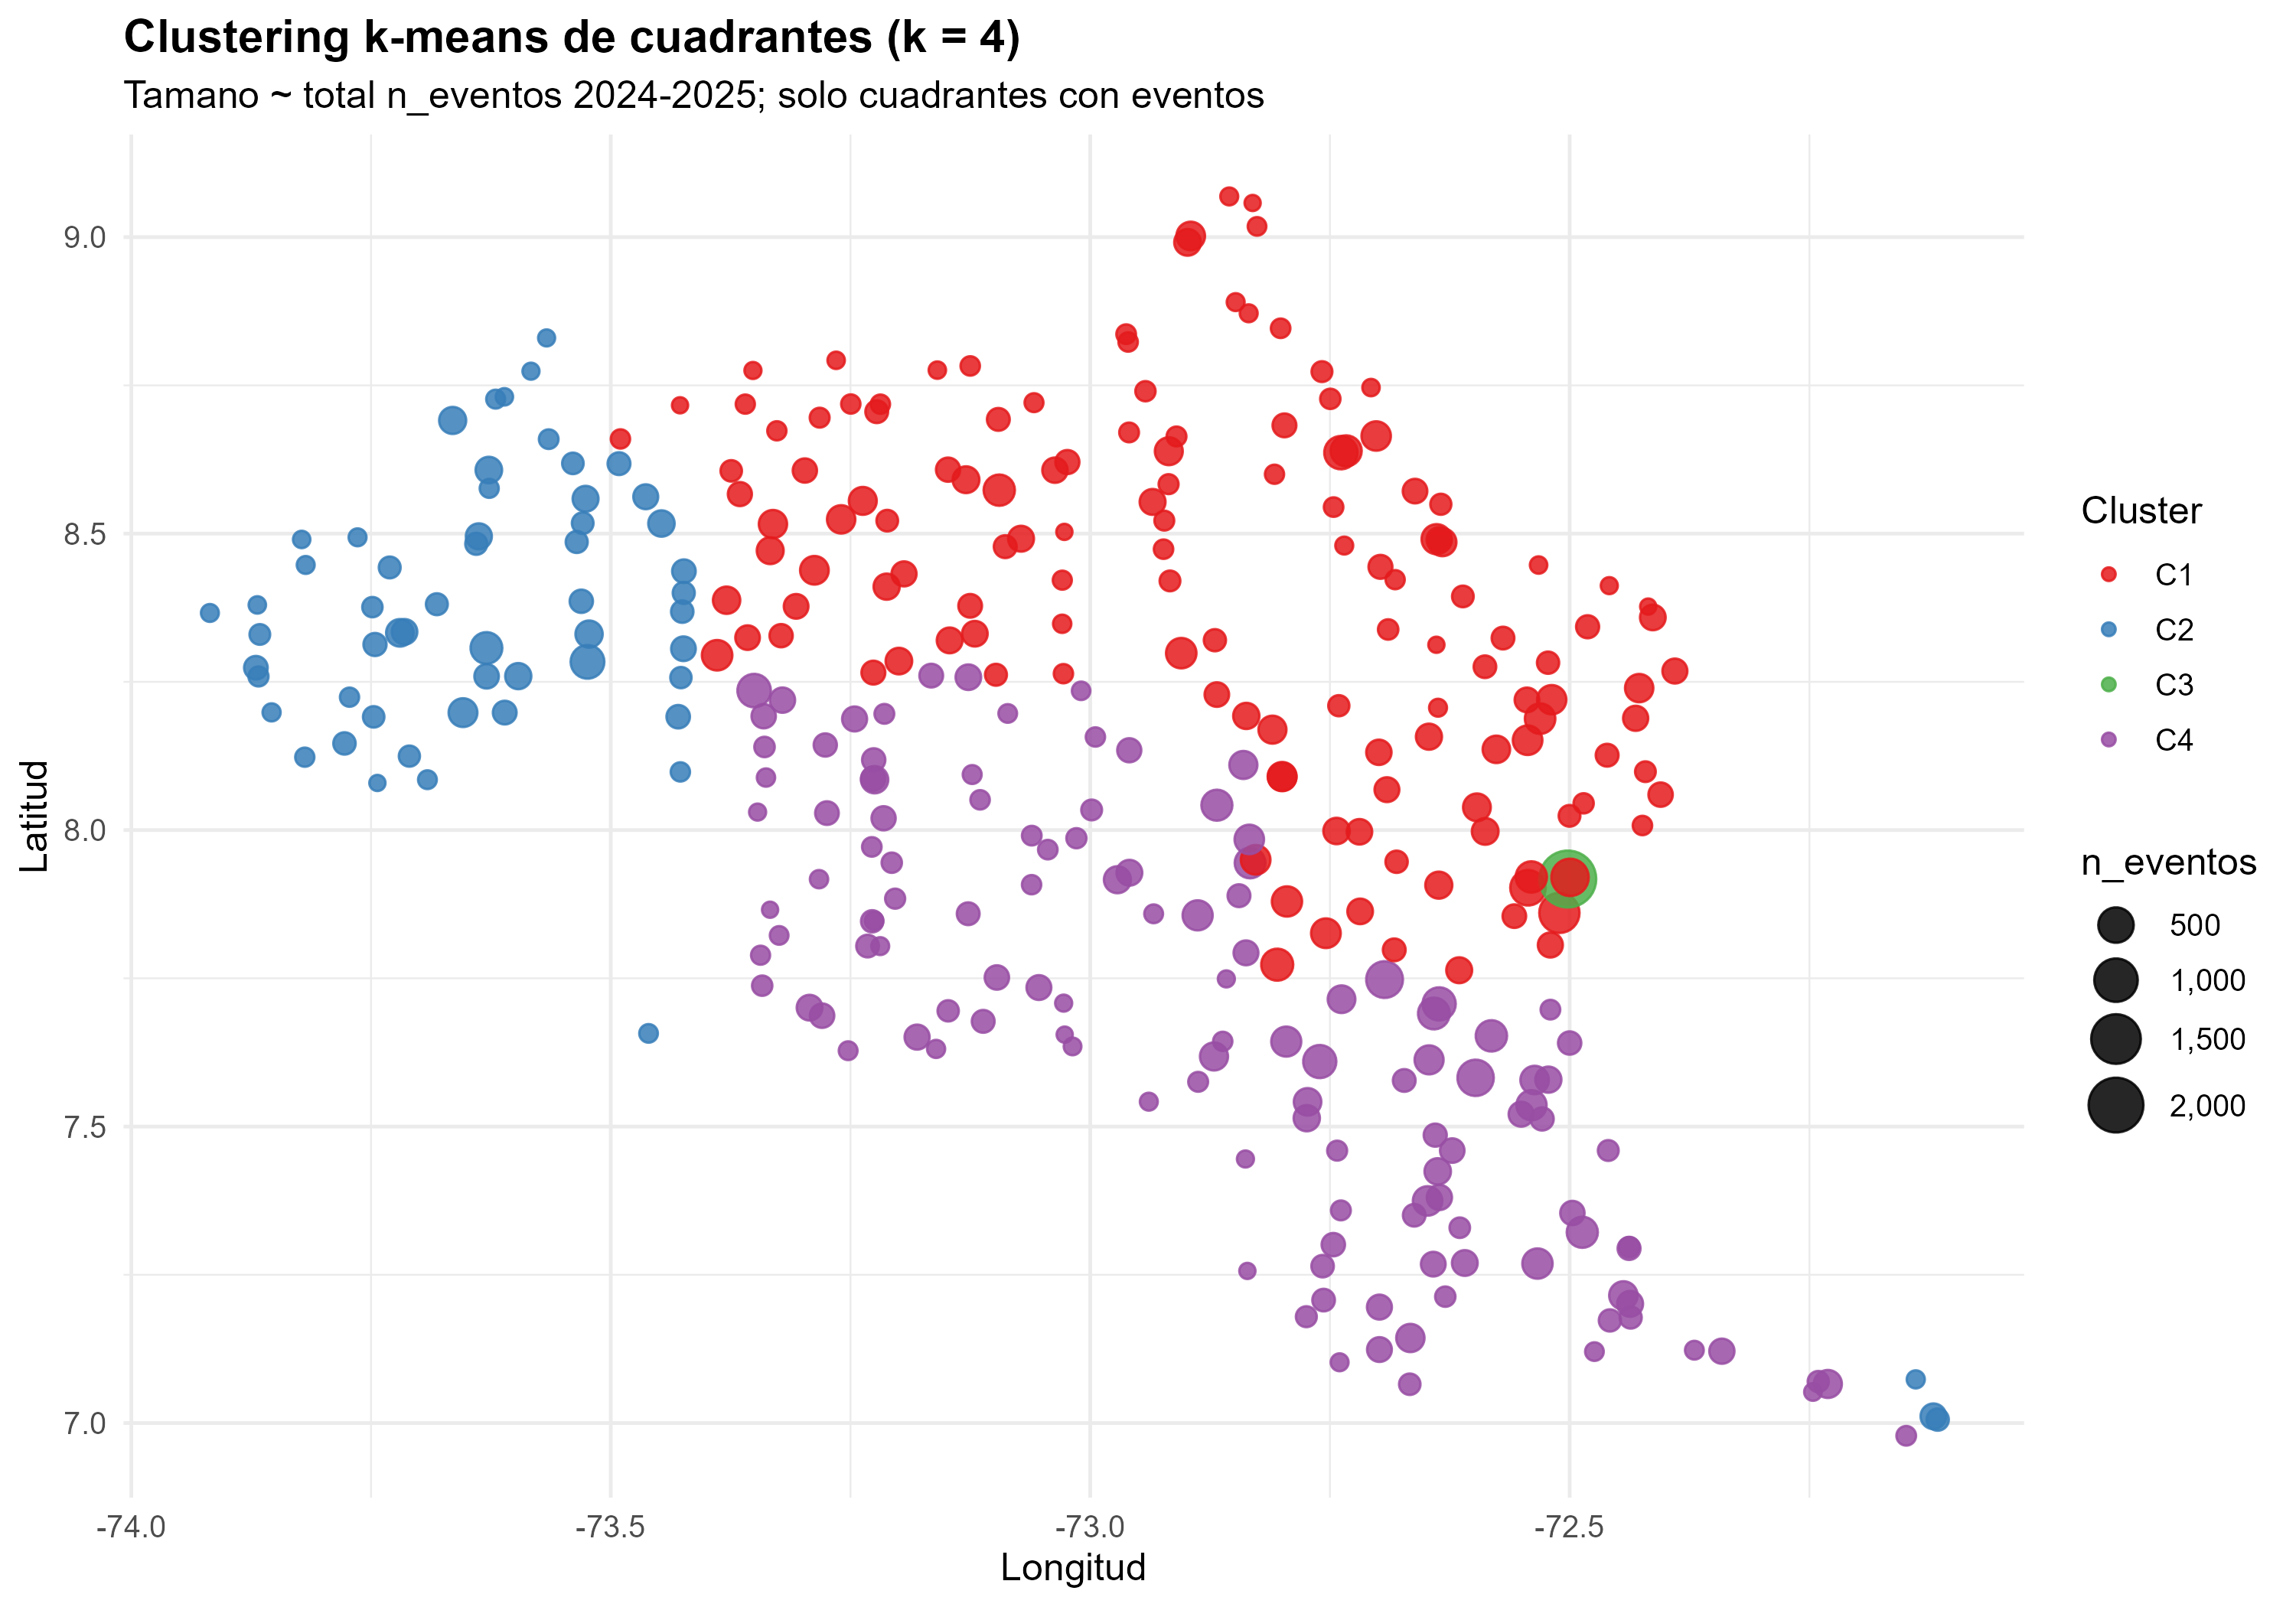
\includegraphics[width=0.95\textwidth]{img/mapa_clusters_cuadrantes_segmentacion_mod.png}
        \caption{Perfiles territoriales de cuadrantes según actividad y clima ($k = 4$; $D_{\mathrm{mod}}$).}
        \label{fig:mapa_cluster_segmentacion}
    \end{figure}
    
    \begin{figure}[!htbp]
        \centering
        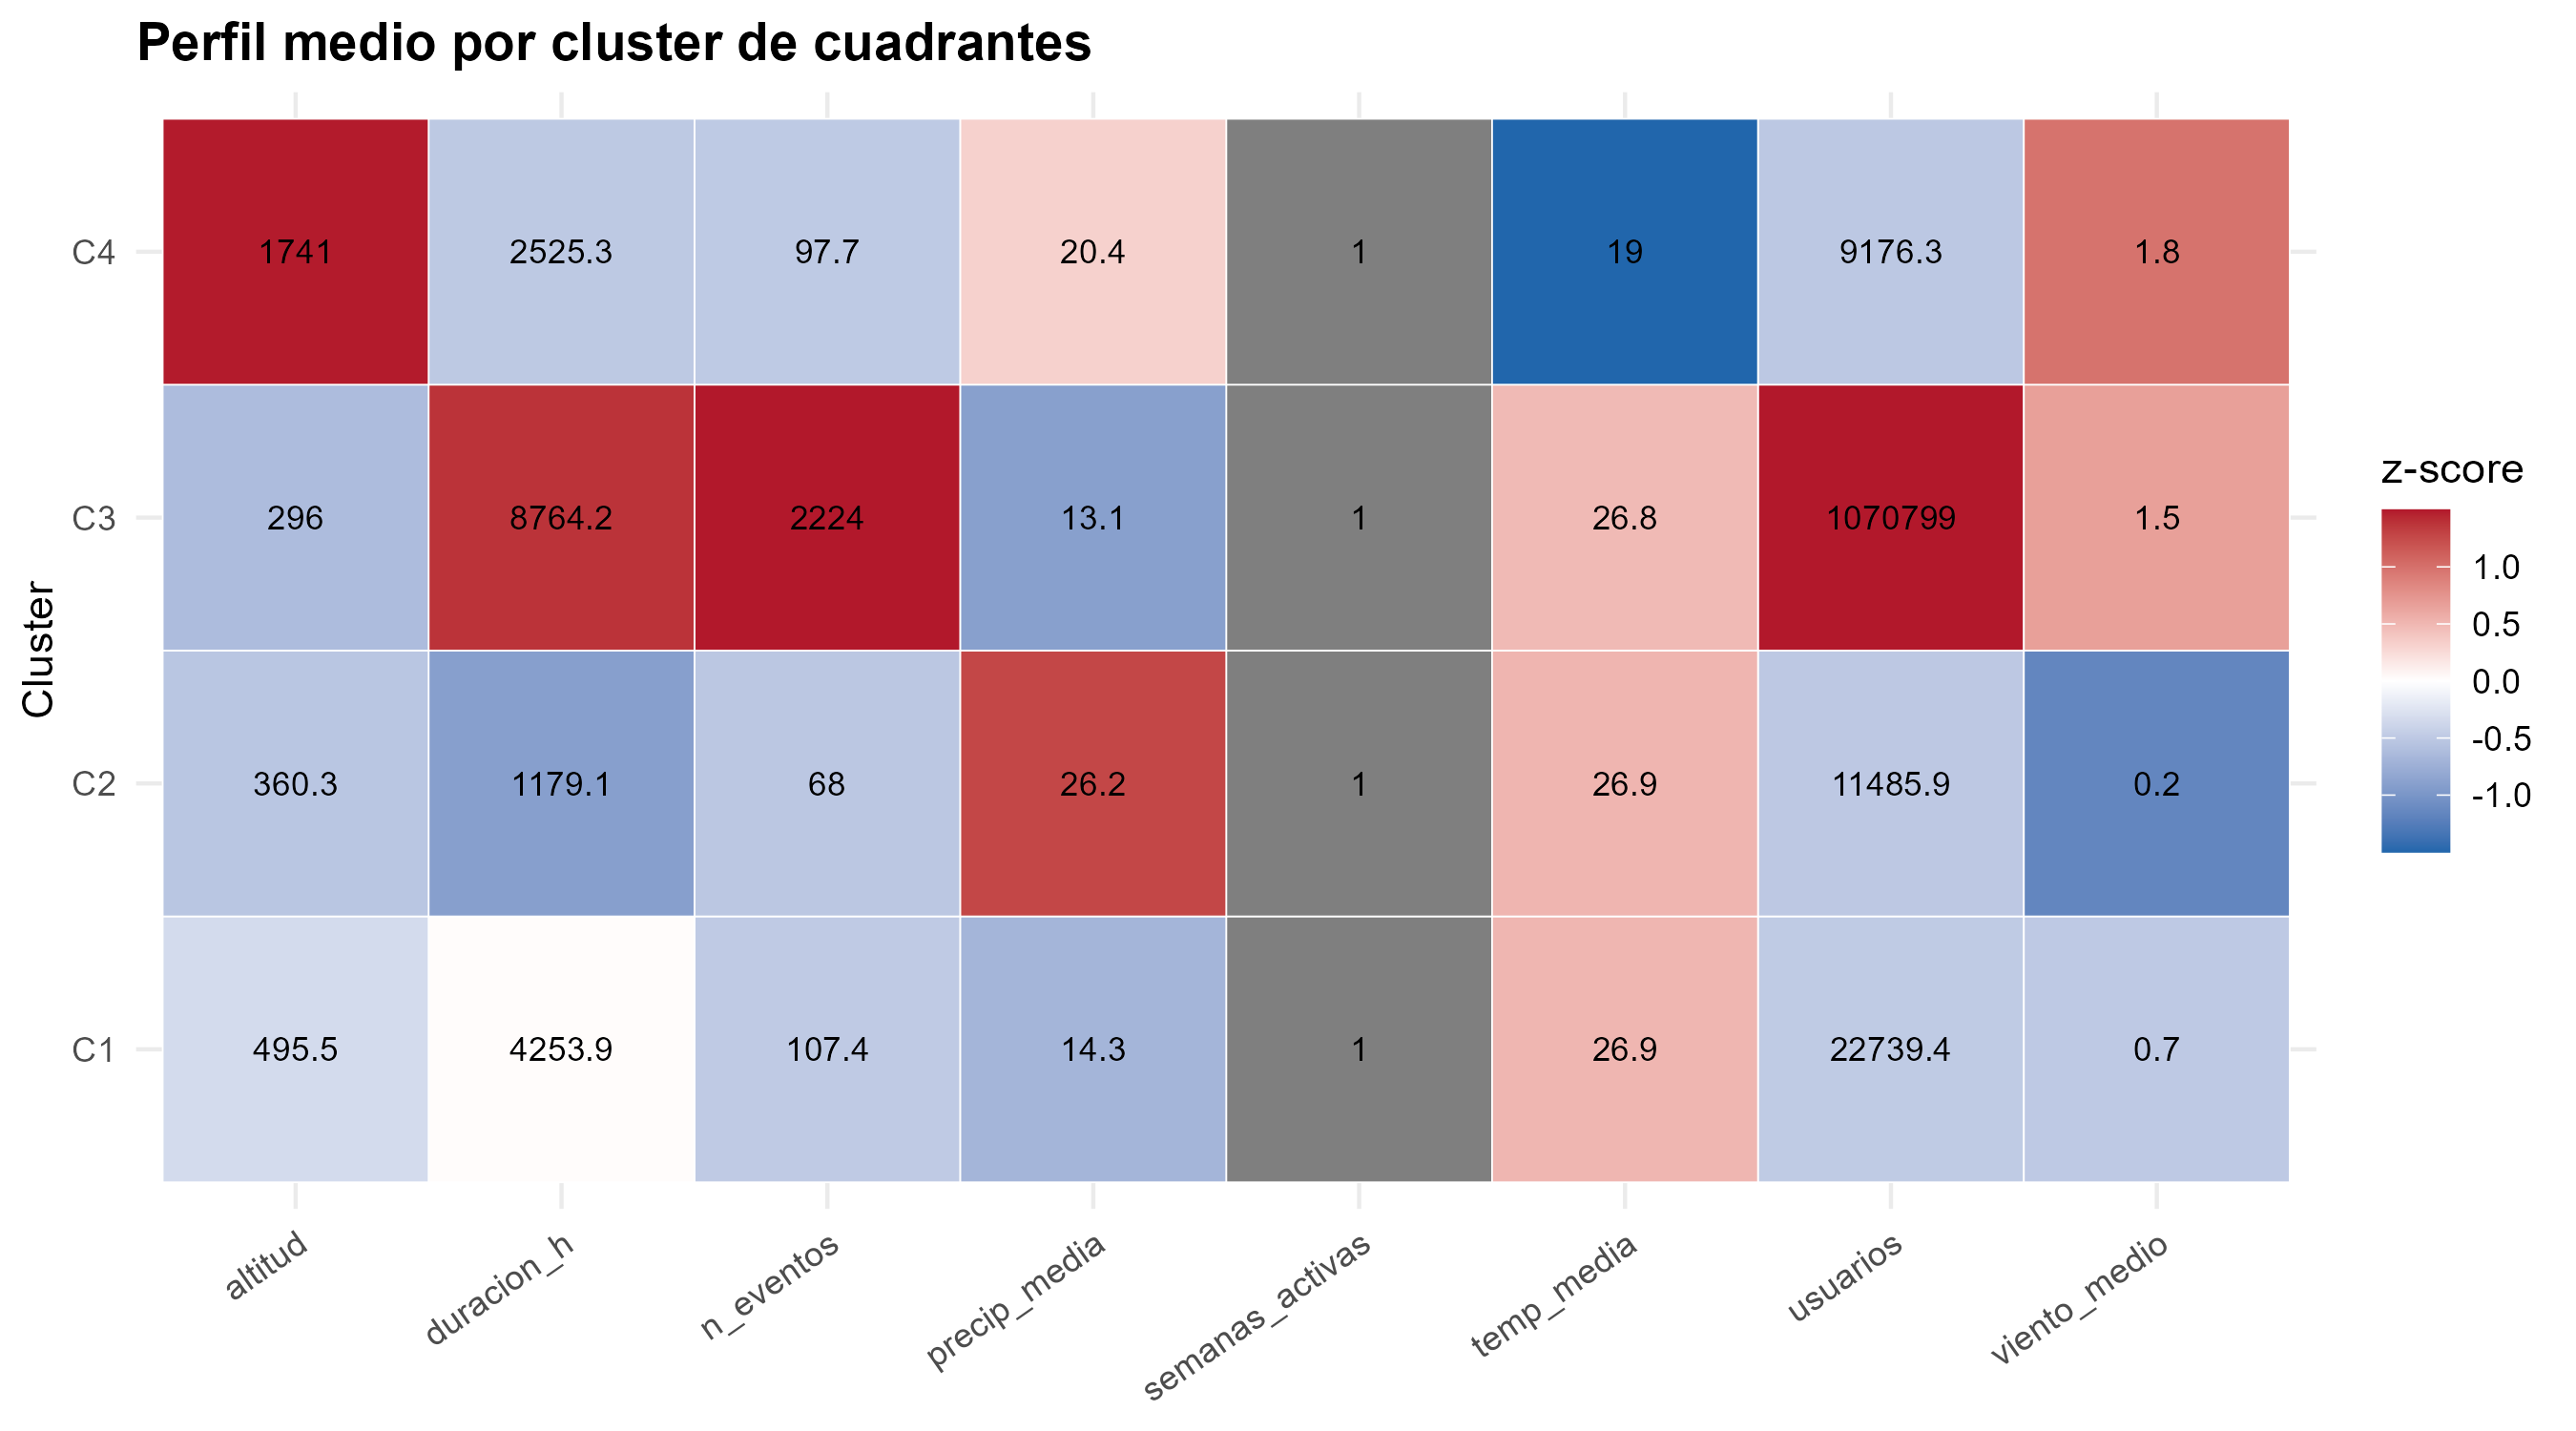
\includegraphics[width=0.88\textwidth]{img/heatmap_perfiles_cluster_segmentacion_mod.png}
        \caption{Perfil medio por cluster de cuadrantes (variables operativas y climáticas).}
        \label{fig:heatmap_cluster_segmentacion}
    \end{figure}
    
    \noindent En síntesis, la segmentación exploratoria sobre $D_{\mathrm{mod}}$ evidencia: (i)~heterogeneidad territorial persistente (14{.}2~\% de cuadrantes en nivel alta concentran actividad desproporcionada); (ii)~incremento homogéneo 2024$\rightarrow$2025 en todos los estratos; (iii)~\textit{ausencia} de diferencia significativa en la frecuencia de interrupciones entre semanas lluviosas y secas cuando la lluvia se mide como acumulado semanal; y (iv)~cuatro perfiles espaciales distinguibles por clustering, ordenados principalmente por severidad y altitud más que por régimen de lluvia. Estos criterios orientan la estratificación territorial y la partición entrenamiento/prueba de la Etapa~4.
    
\subsection{Resultados y entregables de la etapa}
\label{sec:resultados_eda}
    La Etapa~3 sobre $D_{\mathrm{mod}}$ (2024--2025; $36\,120$ filas cuadrante~$\times$~semana) produjo un diagnóstico exploratorio integrado: calidad y distribución de variables (Secciones~\ref{sec:identificacion_datos_faltantes}--\ref{sec:distribucion_variables}), delimitación temporal y materialización del panel de modelado (Sección~\ref{sec:analisis_temporal_eventos}), patrones y visualización (Sección~\ref{sec:identificacion_patrones_tendencias}), correlación bivariada (Sección~\ref{sec:analisis_correlacion_asociacion}), evaluación multivariada con recomendación de predictoras y respuesta (Sección~\ref{sec:evaluacion_multivariada}) y segmentación territorial (Sección~\ref{sec:segmentacion_exploratoria}). Los hallazgos convergentes son: (i)~señal climática contemporánea \textit{débil} en el grano semanal (viento por delante de precipitación); (ii)~\textit{redundancia} en bloques operativo y climático que justifica subconjuntos reducidos, con la severidad (\texttt{usuarios\_afectados}, \texttt{elementos\_afectados}) altamente alineada a \texttt{n\_eventos} en parte por construcción; (iii)~\textit{taxonomía de tres grupos} (Sección~\ref{sec:metodos-modelos}): predictoras disponibles \emph{ex ante}, respuestas $SAIFI$/$SAIDI$, e impacto posterior excluido como predictor contemporáneo; (iv)~\textit{heterogeneidad espacial} y clusters territoriales que sugieren estratificación en el modelado; y (v)~la necesidad de una \textit{partición temporal estricta}, sin muestreo aleatorio, dentro del periodo de cobertura homogénea del emparejamiento evento--elemento. Los informes HTML reproducibles se consolidan en el Apéndice~\ref{app:informes-html}; el \textit{entregable ejecutivo consolidado} corresponde al Apéndice~\ref{app:html-eda} (síntesis de las Secciones~\ref{sec:identificacion_datos_faltantes}--\ref{sec:resultados_eda} con hallazgos, figuras representativas y lineamientos para la Etapa~4). La ingeniería de variables de la Etapa~4 operacionaliza esa taxonomía, incluidos rezagos climáticos y operativos y, si procede, la reelaboración de la métrica de severidad solo con fines descriptivos.
    
    \textit{Resultado:} conocimiento exploratorio del comportamiento de los datos y hallazgos relevantes para el modelado.
    
    \textit{Entregable:} Documento de análisis descriptivo y exploratorio (EDA), Apéndice~\ref{app:html-eda}.
    

\subsection{Síntesis de los hallazgos del análisis exploratorio}
\label{sec:sintesis_eda}


El diagnóstico de completitud sobre la tabla agregada ($N_{\mathrm{agr}} = 90\,128$) no encontró valores faltantes: las $16$ variables registran $0$~\% de datos ausentes y ninguna fila queda incompleta (Sección~\ref{sec:identificacion_datos_faltantes}; Apéndice~\ref{app:html-faltantes-agrupada}, \href{\urlfaltantesagrupada}{informe HTML}). Este resultado no debe interpretarse como ausencia de incompletitud en el proyecto, sino como consecuencia del grano de agregación: los valores ausentes del bloque climático y de \texttt{ALTITUD} se originan en el panel activo~$\times$~día y quedan absorbidos por las reglas de resumen semanal, que operan sobre los días efectivamente disponibles de cada cuadrante. La tabla agregada hereda, por tanto, una completitud estructural que no exige imputación en la Etapa~4, pero cuya interpretación requiere conocer el grano en el que se originó la incompletitud.

El análisis de valores extremos (Sección~\ref{sec:identificacion_valores_extremos}; Apéndice~\ref{app:html-outliers}, \href{\urldetectionoutliers}{informe HTML}) muestra que las variables climáticas diarias tienen baja dispersión relativa (CV entre $0{.}16$ y $0{.}20$) y una proporción marginal de extremos bajo la regla de Tukey, con la precipitación como excepción esperada (CV $=2{.}12$; Tabla~\ref{tab:extremos_clima}). En los días con evento, la severidad y la continuidad muestran alta dispersión relativa y colas pesadas: la duración de interrupción tiene una mediana de $417$ minutos pero un máximo de $332\,395$ minutos (CV $=3{.}56$), y el número de usuarios afectados una mediana de $23$ pero un máximo de $34\,622$ (CV $=3{.}97$; Tabla~\ref{tab:extremos_evento}). Estos extremos se marcan para revisión y tratamiento en la Etapa~4, sin excluirse en esta etapa \pendiente{F1-C9: documentar la regla aplicada y el número de semanas afectadas}.

El análisis de correlación identificó redundancia operativa: los pares \texttt{usuarios\_afectados}--\texttt{elementos\_afectados} ($\rho=0{.}99$), \texttt{n\_eventos}--\texttt{elementos\_afectados} ($\rho=0{.}98$) y \texttt{n\_eventos}--\texttt{usuarios\_afectados} ($\rho=0{.}97$) presentan la mayor asociación del panel (Sección~\ref{sec:analisis_correlacion_asociacion}; Apéndice~\ref{app:html-correlacion}, \href{\urlanalisisCorrelacion}{informe HTML}), en buena parte por construcción compartida desde la misma tabla de eventos. El diagnóstico de multicolinealidad climática (VIF) confirmó inflación severa en el bloque completo de variables meteorológicas (máximo VIF $=43{.}92$ en temperatura media), que se redujo a valores aceptables (máximo $7{.}21$) al restringir el bloque a precipitación, temperatura media, humedad media y viento medio (Sección~\ref{sec:evaluacion_multivariada}; Apéndice~\ref{app:html-multivariado}, \href{\urlanalisisMultivariado}{informe HTML}).

Estas dos redundancias tienen orígenes distintos y exigen tratamientos distintos, distinción que resultó determinante para la Etapa~4. La redundancia operativa es \textit{mecánica}: las cuatro métricas provienen de la misma tabla de eventos, comparten la masa de ceros de las semanas sin interrupción y crecen conjuntamente con el número de eventos, de modo que su correlación no refleja una relación empírica sino la aritmética de la agregación. La redundancia climática es, en cambio, \textit{física}: temperatura media, máxima y mínima miden el mismo fenómeno térmico con resoluciones distintas, y el viento medio y máximo lo propio con el régimen de viento. La primera se resolvió por decisión de rol —fijar la respuesta en los indicadores construidos y excluir la severidad del conjunto predictor—, mientras que la segunda se resolvió por selección de representantes dentro de cada bloque.

En conjunto, estos hallazgos —señal climática contemporánea débil, redundancia en los bloques operativo y climático, y la taxonomía de tres grupos de variables (predictoras \emph{ex ante}, respuestas y variables de impacto posterior; Sección~\ref{sec:metodos-modelos})— definen los criterios de selección de variables aplicados en la ingeniería de la Etapa~4. En particular, la debilidad de la señal climática contemporánea no condujo a descartar el bloque meteorológico, sino a reformular su forma de entrada: lo que el EDA descarta es la utilidad del clima \textit{simultáneo} como predictor, no la del clima acumulado o rezagado, hipótesis que la Etapa~4 operacionaliza mediante \texttt{precip\_ma4} y \texttt{viento\_ma4}. El análisis exploratorio consolidado se documenta en el Apéndice~\ref{app:html-eda} (\href{\urlEDA}{informe HTML}).


\section{Etapa 4 – Resultados de la ingeniería de variables}
\label{sec:resultados-etapa4}

El resultado de esta etapa es el panel analítico final de modelado: un conjunto de predictoras restringido a variables disponibles \emph{ex ante} de la semana a pronosticar (clima rezagado, histórico de eventos, características del cuadrante y estacionalidad), con las variables de impacto posterior (\texttt{usuarios\_afectados}, \texttt{elementos\_afectados}) excluidas explícitamente como predictoras contemporáneas (Sección~\ref{sec:enriquecimiento_panel_cuadrante}). Se incorporaron rezagos espaciales de vecinos (\texttt{SAIDI\_vecinos\_lag1}, \texttt{SAIFI\_vecinos\_lag1}, \texttt{n\_eventos\_vecinos}, \texttt{ndvi\_vecinos}) mediante contigüidad \emph{queen}, y transformaciones logarítmicas $\log(1+\mathrm{SAIDI})$ y $\log(1+\mathrm{SAIFI})$ para estabilizar la varianza de las variables respuesta.

El producto concreto de la etapa es la partición del conjunto de columnas del panel en cuatro clases disjuntas (Sección~\ref{sec:matrices_diseno}; Tabla~\ref{tab:particion_variables_modelado}). Las dos \textbf{variables respuesta} son $\mathrm{SAIDI}$ y $\mathrm{SAIFI}$, estimadas como \texttt{log\_SAIDI1} y \texttt{log\_SAIFI1} en modelos independientes. Las \textbf{predictoras} quedaron en $19$ variables de siete bloques temáticos —clima, vegetación, exposición externa, topología de red, composición socioeconómica, activos y mantenimiento, y dinámica temporal y espacial—, seleccionadas desde un conjunto inicial de $44$ candidatas disponibles en el panel enriquecido. Las \textbf{llaves} (\texttt{id\_cuadrante}, \texttt{semana} y las coordenadas) no actúan como covariables sustantivas sino como índices de absorción en las especificaciones de efectos fijos y como insumo de la matriz de vecindad. Finalmente, el bloque de \textbf{exclusiones deliberadas} comprende las variables de impacto posterior, los insumos contemporáneos de construcción de la respuesta (\texttt{n\_eventos}$_t$, \texttt{duracion\_total}$_t$, admitidos solo rezagados) y la respuesta cruzada contemporánea.

Esta última categoría merece ser reportada como resultado y no solo como decisión de diseño, porque condiciona la lectura de todas las métricas del siguiente apartado. Las variables excluidas no son irrelevantes: \texttt{usuarios\_afectados} presenta la mayor asociación del panel con ambos indicadores, por la razón trivial de que figura en el numerador de su definición (ecuación~\eqref{eq:respuestas_saidi_saifi}). Un modelo que la incorporara como regresor alcanzaría un ajuste próximo a la unidad y sería, sin embargo, inservible: en el momento de pronosticar la semana~$s$ el operador no conoce todavía cuántos usuarios resultarán afectados. El desempeño moderado reportado en la Sección~\ref{sec:resultados-etapa5} es, por tanto, consecuencia directa de haber sostenido la restricción de información y no un indicio de deficiencia del modelado.

La reducción de $44$ a $19$ predictoras se obtuvo mediante la secuencia de filtros descrita en la Sección~\ref{sec:asociacion_depuracion_cuanti}, estimada exclusivamente sobre el conjunto de entrenamiento. En el bloque cuantitativo \emph{ex ante} evaluado de forma independiente sobre $D_{\mathrm{mod}}$, de $27$ candidatas se retuvieron $13$, con el descarte de las temperaturas por redundancia con el eje térmico ya representado y de los promedios móviles del histórico por multicolinealidad con los rezagos simples. En el bloque cualitativo, la depuración concluyó que la información del estrato predominante municipal ya estaba contenida, con mayor resolución, en las proporciones \texttt{prop\_estrato\_*}, por lo que la matriz final privilegia la representación continua. Ninguna variable fue eliminada del panel: la depuración opera sobre la matriz de diseño, de modo que especificaciones alternativas son reconstruibles sin reejecutar la cadena de integración de las Etapas~1 y~2.

La partición temporal quedó documentada en dos niveles consistentes entre sí: la frontera anual 2024/2025, que coincide con el límite natural de $D_{\mathrm{mod}}$, y el \emph{holdout} del $15$~\% final de semanas efectivamente aplicado en la estimación, que sobre las $105$ semanas disponibles reserva aproximadamente las últimas dieciséis. Ambos esquemas son estrictamente cronológicos; en ningún caso se empleó muestreo aleatorio, dada la autocorrelación de $0{.}80$ en el primer rezago sobre $D_{\mathrm{mod}}$.

Este panel, materializado en \texttt{data\_final\_modelo\_cuadrantes\_reales.rds}, constituye el insumo directo para el entrenamiento y la validación de los modelos de la Etapa~5. Su construcción y verificación se documentan en los Apéndices~\ref{app:html-etapa4-01} (\href{\urlEtapaCuatroUno}{informe HTML}), \ref{app:html-etapa4-02} (\href{\urlEtapaCuatroDos}{informe HTML}) y~\ref{app:html-asociacion-cuanti} (\href{\urlasociaciondepuracioncuanti}{informe HTML}).


\section{Etapa 5 – Resultados del modelado predictivo y evaluativo}
\label{sec:resultados-etapa5}

El diagnóstico de dependencia espacial confirmó autocorrelación positiva y significativa tanto en SAIDI (índice de Moran $I=0{.}154$; $p<0{.}001$) como en SAIFI ($I=0{.}179$; $p<0{.}001$), lo que justifica la incorporación de rezagos espaciales entre cuadrantes vecinos y la estimación de modelos espaciales formales (Sección~\ref{sec:metodología-etapa5}; Apéndices~\ref{app:html-etapa5-01}, \href{\urlEtapaCincoUno}{informe HTML}, y~\ref{app:html-etapa5-02}, \href{\urlEtapaCincoDos}{informe HTML}). La magnitud de ambos índices es moderada: una autocorrelación en este rango indica que la vecindad territorial explica una parte identificable pero no dominante de la variación, lo que anticipa el resultado posterior de que SAR y SEM superen al OLS por un margen de AIC estrecho.

La Tabla~\ref{tab:desempeno_saidi} presenta el desempeño en test (escala $\log(1+y)$) de los cuatro modelos de panel semanal para SAIDI. El modelo de efectos fijos de cuadrante~+~semana no resultó evaluable en el conjunto de prueba, ya que las semanas del periodo de prueba no están representadas en el entrenamiento; se reporta explícitamente con valor ausente para dejar constancia de que la especificación fue estimada y de que la imposibilidad de evaluarla es estructural y no una omisión del análisis (Sección~\ref{sec:validacion_modelo}). Entre los modelos evaluables, Random Forest obtiene el menor error (RMSE $=0{.}1195$; MAE $=0{.}0609$; $R^2=0{.}190$), seguido de efectos fijos de cuadrante (RMSE $=0{.}1341$) y Pooled OLS (RMSE $=0{.}1666$).

La progresión de errores entre las tres especificaciones evaluables es interpretable a la luz de la secuencia de relajación de supuestos de la Sección~\ref{sec:seleccion_algoritmos}. El paso de \emph{Pooled} OLS a efectos fijos de cuadrante reduce el RMSE en torno a un $20$~\%, lo que cuantifica cuánta heterogeneidad territorial permanente no estaba capturada por las $19$ covariables observadas: una fracción sustancial de la diferencia entre cuadrantes obedece a factores no medidos y estables en el tiempo. El paso adicional a Random Forest reduce el error en torno a otro $11$~\%, atribuible a no linealidades e interacciones que las especificaciones lineales no representan. Ambas ganancias son reales pero el nivel absoluto de $R^2$ permanece bajo, lo que indica que la componente verdaderamente idiosincrática de la variación semanal no es capturada por ninguna de las familias evaluadas.

\begin{table}[!htbp]
\centering
\small
\caption{Desempeño comparado en test para SAIDI (escala $\log(1+y)$)}
\label{tab:desempeno_saidi}
\begin{tabular}{l r r r}
\toprule
\textbf{Modelo} & \textbf{RMSE} & \textbf{MAE} & \textbf{$R^2$} \\
\midrule
Pooled OLS            & 0.1666 & 0.0627 & 0.0558 \\
FE cuadrante          & 0.1341 & 0.0517 & 0.1087 \\
FE cuadrante+semana   & --     & --     & --     \\
Random Forest         & 0.1195 & 0.0609 & 0.1902 \\
\bottomrule
\end{tabular}
\end{table}

Para SAIFI, la Tabla~\ref{tab:desempeno_saifi} muestra un patrón distinto: el modelo de efectos fijos de cuadrante obtiene el menor error (RMSE $=0{.}0026$), levemente por debajo de Random Forest (RMSE $=0{.}0027$) y de Pooled OLS (RMSE $=0{.}0028$), aunque Random Forest alcanza el mayor $R^2$ ($0{.}234$ frente a $0{.}205$ de FE cuadrante).

Esta divergencia entre métricas dentro del mismo indicador ilustra por qué se reportan las tres conjuntamente (Sección~\ref{sec:evaluacion_desempeno}). Que FE de cuadrante minimice el RMSE mientras Random Forest maximiza el $R^2$ significa que el primero es más preciso en la magnitud predicha y el segundo mejor en el ordenamiento relativo de observaciones: Random Forest identifica con mayor acierto qué cuadrantes-semana tendrán mayor frecuencia de interrupción, pero incurre en desviaciones de magnitud algo mayores. La elección entre ambos depende del uso, y para la frecuencia de interrupciones la especificación paramétrica resulta preferible por su interpretabilidad, dado que su ventaja predictiva frente al modelo no lineal es, en la práctica, inexistente. Nótese además que los valores absolutos de RMSE no son comparables entre SAIFI y SAIDI: ambos se expresan en escala logarítmica sobre indicadores cuyas magnitudes difieren en varios órdenes, por lo que la comparación válida es siempre intra-indicador.

Las Figuras~\ref{fig:saidi_pred_obs} y~\ref{fig:saifi_pred_obs} contrastan los valores observados y predichos del mejor modelo de cada indicador en el conjunto de prueba, y las Figuras~\ref{fig:saidi_rf_imp} y~\ref{fig:saifi_rf_imp} presentan la importancia de las variables en los modelos Random Forest.

\begin{figure}[!htbp]
    \centering
    \includegraphics[width=0.82\textwidth]{img/saidi_pred_vs_obs.png}
    \caption{Valores observados frente a predichos de $SAIDI$ en el conjunto de prueba (escala $\log(1+y)$).}
    \label{fig:saidi_pred_obs}
\end{figure}

\begin{figure}[!htbp]
    \centering
    \includegraphics[width=0.82\textwidth]{img/saifi_pred_vs_obs.png}
    \caption{Valores observados frente a predichos de $SAIFI$ en el conjunto de prueba (escala $\log(1+y)$).}
    \label{fig:saifi_pred_obs}
\end{figure}

\begin{figure}[!htbp]
    \centering
    \includegraphics[width=0.90\textwidth]{img/saidi_rf_importancia.png}
    \caption{Importancia de variables (\%IncMSE) del Random Forest para $SAIDI$.}
    \label{fig:saidi_rf_imp}
\end{figure}

\begin{figure}[!htbp]
    \centering
    \includegraphics[width=0.90\textwidth]{img/saifi_rf_importancia.png}
    \caption{Importancia de variables (\%IncMSE) del Random Forest para $SAIFI$.}
    \label{fig:saifi_rf_imp}
\end{figure}


\begin{table}[!htbp]
\centering
\small
\caption{Desempeño comparado en test para SAIFI (escala $\log(1+y)$)}
\label{tab:desempeno_saifi}
\begin{tabular}{l r r r}
\toprule
\textbf{Modelo} & \textbf{RMSE} & \textbf{MAE} & \textbf{$R^2$} \\
\midrule
Pooled OLS            & 0.0028 & 0.0011 & 0.1252 \\
FE cuadrante          & 0.0026 & 0.0009 & 0.2052 \\
FE cuadrante+semana   & --     & --     & --     \\
Random Forest         & 0.0027 & 0.0012 & 0.2343 \\
\bottomrule
\end{tabular}
\end{table}

Para la explicación estructural en corte transversal, se agregó cada indicador como promedio ponderado por cuadrante a lo largo de todo el periodo 2024--2025 ($N=343$ cuadrantes), y se compararon por AIC los modelos OLS, SAR y SEM sobre ese corte transversal. El AIC favoreció a SAR para SAIDI (AIC $=-1305{.}19$, frente a $-1299{.}80$ de OLS) y a SEM para SAIFI (AIC $=-4267{.}92$, frente a $-4266{.}05$ de OLS), en ambos casos por una diferencia moderada que refleja una autocorrelación espacial real pero no dominante en los residuos \pendiente{verificar AIC de OLS con C7 y reportar $\rho$, $\lambda$ y Moran de residuos}.

Es importante precisar que los modelos espaciales SAR/SEM no reportan un $R^2$ en el sentido clásico. La capacidad explicativa del bloque de predictoras --infraestructura de red, antigüedad de activos, composición de estrato y exposición territorial-- se cuantificó mediante la regresión lineal equivalente sobre el mismo corte transversal de $343$ cuadrantes, usada como verificación de robustez frente a colinealidad estructural: $R^2=0{.}901$ para SAIDI (Tabla~\ref{tab:cross_section_saidi}) y $R^2=0{.}837$ para SAIFI tras selección \emph{stepwise} (Tabla~\ref{tab:cross_section_saifi}), ambos con significancia empírica confirmada por prueba de permutación ($p<0{.}001$). Este $R^2$ no debe compararse directamente con el de las Tablas~\ref{tab:desempeno_saidi} y~\ref{tab:desempeno_saifi}: mientras estas últimas evalúan la predicción de observaciones semanales individuales en test ($N=2\,215$, con toda la variabilidad semana a semana), el corte transversal explica el promedio de cada cuadrante a lo largo de $\sim 105$ semanas ($N=343$), un objetivo distinto y estadísticamente más simple porque el promediado reduce el ruido idiosincrático. En síntesis, la red tiene un patrón espacial altamente explicable por infraestructura y exposición territorial, pero la magnitud semana a semana conserva incertidumbre irreducible que ningún modelo aquí evaluado elimina por completo.

\begin{table}[!htbp]
\centering
\small
\caption{Regresión de corte transversal para SAIDI promedio por cuadrante ($N=343$; $R^2=0{.}901$)}
\label{tab:cross_section_saidi}
\begin{tabular}{l r r}
\toprule
\textbf{Predictor} & \textbf{Coeficiente} & \textbf{valor $p$} \\
\midrule
n\_elementos                  & $4{.}39\times10^{-4}$  & $<0{.}001$ \\
longitud\_red\_km             & $-8{.}08\times10^{-4}$ & $<0{.}001$ \\
edad\_activo\_mas\_viejo\_anios & $-2{.}76\times10^{-2}$ & $<0{.}001$ \\
ndvi\_promedio                & $7{.}59\times10^{-2}$  & $0{.}007$ \\
prop\_transformadores, densidad\_terminales, prop\_estrato\_1/2, prop\_no\_residencial, PROM\_CANT\_MODIFICACIONES, dist\_sismo\_prom\_km, precip\_promedio & no significativos & $>0{.}10$ \\
\bottomrule
\end{tabular}
\end{table}

\begin{table}[!htbp]
\centering
\small
\caption{Regresión de corte transversal para SAIFI promedio por cuadrante, modelo \emph{stepwise} ($N=343$; $R^2=0{.}837$)}
\label{tab:cross_section_saifi}
\begin{tabular}{l r r}
\toprule
\textbf{Predictor} & \textbf{Coeficiente} & \textbf{valor $p$} \\
\midrule
n\_elementos                  & $3{.}65\times10^{-6}$  & $<0{.}001$ \\
longitud\_red\_km             & $-3{.}98\times10^{-6}$ & $0{.}018$ \\
edad\_activo\_mas\_viejo\_anios & $-1{.}14\times10^{-4}$ & $0{.}057$ \\
dist\_sismo\_prom\_km         & $7{.}51\times10^{-6}$  & $0{.}011$ \\
\bottomrule
\end{tabular}
\end{table}

La importancia de variables del Random Forest y estas regresiones de corte transversal coinciden en señalar como predictores más relevantes: el número de elementos de red y la longitud de red del cuadrante, la edad del activo más antiguo, y de forma secundaria la exposición sísmica (SAIFI) y el NDVI (SAIDI). \pendiente{F1-C2: reescribir la triangulación con una tabla de variables por modelo; en la especificación actual \texttt{n\_elementos} no forma parte de las predictoras del panel semanal, por lo que la convergencia solo puede afirmarse para las variables comunes a ambos modelos (p.\,ej., \texttt{longitud\_red\_km} y la antigüedad de los activos).}

Dos signos merecen comentario porque podrían leerse como contraintuitivos. El coeficiente de \texttt{longitud\_red\_km} es negativo en ambos indicadores, pese a que una red más extensa expone más activos a falla. La explicación plausible es que la longitud de red, condicionada al número de elementos ya incluido en la especificación, deja de medir exposición y pasa a aproximar el carácter rural y disperso del cuadrante: a igual número de activos, mayor longitud implica menor densidad de usuarios por kilómetro y, por tanto, menor contribución al indicador, que se pondera por usuarios afectados. El coeficiente negativo de \texttt{edad\_activo\_mas\_viejo\_anios} admite una lectura análoga: la variable se construye sobre la última fecha de modificación registrada, de modo que un valor alto señala un activo sin intervenciones recientes, lo que en zonas de baja criticidad operativa puede coincidir con menor exposición antes que con mayor deterioro. Ambas interpretaciones son plausibles pero no verificadas con los datos disponibles, y se señalan como hipótesis a contrastar en trabajo posterior. En síntesis: \textbf{para pronóstico semanal, Random Forest es el modelo recomendado para SAIDI y efectos fijos de cuadrante para SAIFI}; \textbf{para explicación del patrón espacial promedio, SAR (SAIDI) y SEM (SAIFI) son los modelos preferidos por AIC}, con una capacidad explicativa alta y verificada como no artefactual cuando se cuantifica mediante su regresión lineal equivalente.


\section{Etapa 6 – Síntesis general y cierre frente a los objetivos}
\label{sec:resultados-etapa6}

El proyecto recorrió las seis etapas metodológicas descritas en el Capítulo~\ref{sec:metodologia} y produjo, de forma trazable y reproducible, un flujo completo desde la extracción de datos crudos hasta modelos predictivos y estructurales validados para SAIDI y SAIFI. La Tabla~\ref{tab:sintesis_etapas} resume el resultado principal de cada etapa.

\begin{table}[!htbp]
\centering
\small
\caption{Síntesis de resultados por etapa metodológica}
\label{tab:sintesis_etapas}
\begin{tabular}{p{0.20\textwidth} p{0.72\textwidth}}
\toprule
\textbf{Etapa} & \textbf{Resultado principal} \\
\midrule
Etapa 1 & Seis fuentes consolidadas (BRAE, OMS SPARD/SP7, GIS, NASA POWER); $95\,280$ eventos depurados y $83{.}5$ millones de registros climáticos. \\
Etapa 2 & Panel activo--día ($N=87\,007\,074$) y panel cuadrante--semana ($N_{\mathrm{agr}}=90\,128$); detección de un sesgo sistemático de emparejamiento 2021--2023 que delimitó el dataset de modelado $D_{\mathrm{mod}}$ (2024--2025). \\
Etapa 3 & Sin datos faltantes en la tabla agregada; redundancia identificada entre severidad y frecuencia; señal climática contemporánea débil; multicolinealidad climática corregida (VIF máximo de $43{.}92$ a $7{.}21$). \\
Etapa 4 & Panel analítico final con partición explícita de columnas: $2$ respuestas ($\mathrm{SAIDI}$, $\mathrm{SAIFI}$ en escala $\log(1+y)$), $19$ predictoras \emph{ex ante} seleccionadas de $44$ candidatas, llaves de identificación y un bloque de exclusiones deliberadas (impacto posterior y respuesta cruzada contemporánea); rezagos temporales y espaciales de vecinos construidos sin fuga de información. \\
Etapa 5 & Random Forest (SAIDI) y FE cuadrante (SAIFI) como mejores modelos de pronóstico semanal; SAR (SAIDI) y SEM (SAIFI) preferidos por AIC como modelos estructurales, con capacidad explicativa verificada como robusta ($R^2>0{.}83$ en la regresión de corte transversal equivalente); autocorrelación espacial significativa en ambos indicadores (Moran's $I$). \\
Etapa 6 & Documentación reproducible de las seis etapas en informes HTML con URL estable (Apéndice~\ref{app:informes-html}) y código fuente de extracción e integración (Apéndice~\ref{app:codigo}), con trazabilidad verificable entre cada afirmación del documento y su evidencia computacional. \\
\bottomrule
\end{tabular}
\end{table}

La Tabla~\ref{tab:cierre_objetivos} articula estos resultados con los tres objetivos específicos del proyecto (Sección~\ref{sec:objetivos}), evidenciando su cumplimiento.

\begin{table}[!htbp]
\centering
\small
\caption{Cierre de resultados frente a los objetivos específicos}
\label{tab:cierre_objetivos}
\begin{tabular}{p{0.32\textwidth} p{0.60\textwidth}}
\toprule
\textbf{Objetivo específico} & \textbf{Resultado que lo responde} \\
\midrule
1. Consolidar las fuentes de datos relevantes, documentando cobertura, calidad y limitaciones mediante un catálogo de datos y métricas de integridad. &
Tabla de linaje de datos (Tabla~\ref{tab:data_lineage}) con las seis fuentes, sus reglas de depuración y su resultado; diagnóstico de completitud sin valores faltantes; identificación y documentación explícita del sesgo de cobertura 2021--2023 como limitación conocida (Sección~\ref{sec:resultados-etapa2}). \\
2. Determinar qué variables operativas, técnicas y climáticas son más relevantes para predecir SAIDI y SAIFI mediante modelos estadísticos o de Machine Learning. &
Importancia de variables del Random Forest y coeficientes de los modelos espaciales (Sección~\ref{sec:resultados-etapa5}): infraestructura de red (número de elementos, longitud de red), antigüedad de activos, composición de estrato y clientes no residenciales, exposición sísmica y vegetación (NDVI), además de la autocorrelación espacial confirmada por el índice de Moran. \\
3. Evaluar el desempeño de diferentes métodos estadísticos o de Machine Learning para predecir SAIDI y SAIFI por circuito o zona. &
Comparación de cuatro algoritmos de panel (Pooled OLS, FE cuadrante, FE cuadrante+semana, Random Forest) más dos modelos espaciales formales (SAR, SEM) para cada indicador, con métricas de desempeño en test (RMSE, MAE, $R^2$) y AIC (Tablas~\ref{tab:desempeno_saidi} y~\ref{tab:desempeno_saifi}), identificando el mejor modelo de pronóstico y el mejor modelo estructural para cada indicador. \\
\bottomrule
\end{tabular}
\end{table}

